% Engineering, master and phd degree 
%PROPOSAL(PROTOCOL) format, April 2021, for the 
%**Instituto Tecnológico de Morelia**
%-=-=-=-=-=-=-=-=-=-=-=-=-
% 1)Configuration:
\documentclass[listings,drafting,spanish]{itmthesis} %itm thesis class
%!TeX root=./thesisStructure.tex
%Add here the packages, variables, definitions, environments and specific elements created only for your thesis

% 1 Code listing setup
%------------------
\RequirePackage{listings}
\RequirePackage{xcolor}
\definecolor{gray97}{gray}{0.97}
\definecolor{gray45}{gray}{0.45}
\newcaptionname{spanish}{\lstlistlistingname}{Sección de Códigos}
\renewcommand{\lstlistingname}{Código}
\renewcommand{\lstlistlistingname}{Códigos}
\lstset{ frame=Ltb,
     framerule=0pt,
     aboveskip=0.2cm,
     framextopmargin=3pt,
     framexbottommargin=3pt,
     framexleftmargin=0.4cm,
     framesep=0pt,
     rulesep=.4pt,
     backgroundcolor=\color{gray97},
     rulesepcolor=\color{black},
     %
     stringstyle=\ttfamily,
     showstringspaces = false,
     %basicstyle=\small\ttfamily,
     %basicstyle=\small,
     commentstyle=\color{gray45}\ttfamily,
     keywordstyle=\bfseries,
     %
     numbers=left,
     numbersep=15pt,
     numberstyle=\tiny,
     numberfirstline = false,
     breaklines=true,
   }

% 2 Commands and variables
% 2.1 Thesis's title page config
%------------------
\newcommand{\myTitle}{Modelo basado en inteligencia artificial para la estimación de la calidad del agua a partir del estudio de parámetros fisicoquímicos en procesos de potabilización}
\newcommand{\mySubtitle}{Caso de Estudio a Nivel Maestría}
\newcommand{\myDegree}{Maestro en Ciencias en Ingeniería Electrónica}
% 2.2 Autores:
\newcommand{\myName}{Bryan Martín Miranda Leal}
\newcommand{\myNumber}{M16121395}
%\newcommand{\myPartner}{Otro autor}
%----------------
% 2.3 Mesa de revisión
%Director:
\newcommand{\myProf}{Gerardo Marx Chávez Campos}
%Codirector:
\newcommand{\myOtherProf}{Adriana del Carmen Téllez Anguiano\xspace}
%Revisor 1:
\newcommand{\mySupervisor}{Arturo Rangel Gonce\xspace}
%Revisor 2:
\newcommand{\myOtherSupervisor}{María del Carmen Cano Correa\xspace}
%--------------
% 2.4 Datos del instituto:
\newcommand{\myFaculty}{Maestría en Ciencias en Ingeniería Electrónica}
\newcommand{\myDepartment}{División de Estudios de Posgrado e Investigación}
\newcommand{\myUni}{Instituto Tecnológico de Morelia}
\newcommand{\myLocation}{Morelia, Michoacán, México}
\newcommand{\myTime}{Junio 2025}
\newcommand{\myThesisVersion}{Rev 2.0}

%---------------------
% 3	USEFUL COMMANDS
%---------------------
\newcommand{\ie}{i.\,e.}
\newcommand{\Ie}{I.\,e.}
\newcommand{\eg}{e.\,g.}
\newcommand{\Eg}{E.\,g.}


%-------------------------
% 4. Required packages for
% figures, plots, subfigures
%-------------------------
\usepackage{float}
\usepackage{subfigure}
\usepackage{tikz}
\usepackage{booktabs} %Beautiful tables
\usepackage{todonotes} %Todo list for comments
\usepackage[version-1-compatibility]{siunitx} %easy writting of SI units
\usepackage{pgfplots}
\pgfplotsset{compat=1.10}
\decimalpoint %Decimal point enable
\usepackage[acronym]{glossaries}
%-------------------------
% 5. setting space for indentation
% space between paragraphs and
% baseline.
% Uncomment to set parameters
%-------------------------
% \setlength{\parindent}{4em}
\setlength{\parskip}{0.5em}
%\renewcommand{\baselinestretch}{2.0} % Interlineado
% configuration and packages
%!TeX root=../thesisStructure.tex
\makeglossaries
\newglossaryentry{latex}
{
    name=latex,
    description={Es un lenguaje de marcado o sintaxis especialmente diseñado para documentos científicos}
}

\newglossaryentry{maths}{
	name=matemáticas,
  description={Las matemáticas son sólo una aproximación a la realidad de la vida}}

\newglossaryentry{formula}{
	name=formula,
	description={A mathematical expression}}


\newacronym{ecm}{ECM}{Error Cuadrático Medio}

\newacronym{ls}{LS}{Mínimos Cuadrados, \textit{Least Squares}}

%\usepackage{tikz}
%\usetikzlibrary{shapes.geometric, arrows}
\usetikzlibrary{shapes, arrows}

\usepackage{pstricks,pst-node}

\usepackage[outline]{contour} % glow around text
\usepackage{xcolor}
\usepackage{tikz}
\usepackage{listofitems} % for \readlist to create arrays
\tikzstyle{neuron}=[thick,draw=blue,fill=blue!20,circle,minimum size=22]
\tikzstyle{input}=[thick,draw=green,fill=green!20,circle,minimum size=22]
\tikzstyle{output}=[thick,draw=red,fill=red!20,circle,minimum size=22]
\tikzstyle{connect}=[->,thick,shorten >=1]


\begin{document}
% -=-=-=-=-=-=-=-=-=-=-=-=-
% 2)Front Matter:
\pagenumbering{roman} % Roman page numbering 
%----------------------------
% Thesis's precontents
%--------------------------
%Titlepage:
%% Portada Ingeniería:
\pdfbookmark[1]{Portada}{Portada} % Bookmark name visible in a PDF viewer 
\begin{titlepage}
\begin{addmargin}[-1cm]{-3cm}
\hfill

\begingroup
%Logotipos:
\begin{picture}(0,0)
\put(-10,-20){
\includegraphics[width=7cm]{logos/sepLogo.jpg}}
\put(200,-20){\includegraphics[width=5cm]{logos/tecnmBW}}
\put(380,-20){
\includegraphics[width=3cm]{logos/itm}}
\end{picture}

\begin{center}
%{\scshape\LARGE SECRETAR\'IA DE EDUCACI\'ON P\'UBLICA\\

\vspace{0.1in}
\end{center}
\endgroup
%--------------
\begin{center}
\bigskip
\rule[3mm]{160mm}{4pt}
\rule[3mm]{140mm}{3pt}\\
\bigskip
\begingroup
{\Huge
\textsc{\myUni}\\\vspace{0.1in}
{\Huge
\calligra{``José María Morelos y Pavón''}}}
\endgroup
\end{center}
%-------Datos de portada-------
\begingroup % Create the command for including the title page in the document
\hbox{ % Horizontal box
\hspace*{.01\textwidth} % Whitespace to the left of the title page
%\rule[depth]{width}{height}
\rule[-1cm]{6pt}{15cm} % Vertical line
\hspace{3mm}%Horizontal space 
\rule[0cm]{3pt}{14cm}%
\hspace{3mm}
\rule[2cm]{2pt}{12cm} 
\hspace{1cm}
\parbox[b]{.75\textwidth}{ % Texto de la portada aquí:
\begin{center}
%-----------
	{\Large
	\scshape{\myDepartment}\\
	\textsc{\myFaculty} \\ \bigskip}

	\textsc{TESIS}\\\bigskip
	\begingroup
		% Título de la tesis:
		{\Large
		\textsc{\color{Maroon}\textsc{``\myTitle''}}\\  
		\bigskip
		\bigskip
		%Subtítulo de la tesis:
		{\color{Maroon}\texttt{\mySubtitle}}}
	\endgroup
	
	\bigskip 
	\bigskip 
	\bigskip
	
	\textsc{QUE PARA OBTENER EL TÍTULO DE:}\\
	\bigskip
	{\large\textsc{\myDegree}\\\bigskip}
	\textsc{PRESENTA:}\\
	{\large\textsc{\myName}}\\ % Your name
	%\textsc{\mytwoName} \\
	\bigskip
	\bigskip
	{\large
	\textsc{Director: \myProf}\\
	\textsc{Codirector: \myOtherProf}\\
	\textsc{Revisor: \mySupervisor}\\
	\textsc{Revisor: \myOtherSupervisor}\\}
\end{center}}}
\endgroup
\bigskip
\bigskip
\bigskip
\begin{center}
\textsc{\myLocation \, -- \myTime \, -- \myThesisVersion}
\end{center}
\end{addmargin}
\end{titlepage} %ing
%!TeX root=../thesisStructure.tex
% Portada Maestría/Doctorado:
\pdfbookmark[1]{Portada}{Portada} % Bookmark name visible in a PDF viewer 
\begin{titlepage}
\begin{addmargin}[-1cm]{-3cm}
\hfill

\begingroup
%Logotipos:
\begin{picture}(0,0)
%\put(-10,-20){
\includegraphics[width=7cm]{sepLogo.jpg}}
%\put(-10,-65){
\includegraphics[width=7cm,height=5.7cm]{imgss152.jpg}}

%\put(-10,-20){
\includegraphics[scale=1.1]{imgss153.png}}
\put(-10,-10){
\includegraphics[scale=0.15]{imgss223.jpg}}
\put(200,-20){\includegraphics[width=5cm]{tecnmBW}}
\put(380,-20){
\includegraphics[width=3cm]{itm}}

%\put(380,-20){\includegraphics[width=3cm]{whiteLogo.PNG}}
\end{picture}

\begin{center}
%{\scshape\LARGE SECRETAR\'IA DE EDUCACI\'ON P\'UBLICA\\

\vspace{0.1in}
\end{center}
\endgroup
%--------------
\begin{center}
\bigskip
\rule[3mm]{160mm}{4pt}
\rule[3mm]{140mm}{3pt}\\
\bigskip
\begingroup
{\Huge
\textsc{\myUni}\\\vspace{0.1in}
{\Huge
\calligra{``José María Morelos y Pavón''}}}
\endgroup
\end{center}
%-------Datos de portada-------
\begingroup % Create the command for including the title page in the document
\hbox{ % Horizontal box
\hspace*{.01\textwidth} % Whitespace to the left of the title page
%\rule[depth]{width}{height}
\rule[-1cm]{6pt}{15cm} % Vertical line
\hspace{3mm}%Horizontal space 
\rule[0cm]{3pt}{14cm}%
\hspace{3mm}
\rule[2cm]{2pt}{12cm} 
\hspace{1cm}
\parbox[b]{.75\textwidth}{ % Texto de la portada aquí:
\begin{center}
%-----------
	{\Large
	\scshape{\myDepartment}\\
	\textsc{\myFaculty} \\ \bigskip}

	\textsc{TESIS}\\\bigskip
	\begingroup
		% Título de la tesis:
		{\Large
		\textsc{\color{Maroon}\textsc{``\myTitle''}}\\  
		%\bigskip
		\bigskip
		%Subtítulo de la tesis:
		%{\color{Maroon}\texttt{\mySubtitle}}
		}
	\endgroup
	%\bigskip
	\textsc{QUE PARA OBTENER EL GRADO DE:}\\
	%\bigskip
	{\large\textsc{\myDegree}\\\bigskip}
	\textsc{PRESENTA:}\\
	{\large\textsc{\myName}}\\\bigskip % Your name
	%\textsc{\mytwoName} \\
    %\vspace{4mm}
	{\large
	\textsc{Director: \myProf}\\
	\textsc{Codirector: \myOtherProf}\\
	\textsc{Revisor: \mySupervisor}\\
	\textsc{Revisor: \myOtherSupervisor}\\}
	\bigskip
	%\bigskip
	\bigskip
	%\bigskip
	%\bigskip
	\textsc{\myLocation \, -- \myTime \, -- \myThesisVersion}
\end{center}}}
\endgroup
\end{addmargin}
\end{titlepage} %MC
%Back of the title page:
%!TeX root=../thesisStructure.tex
% Back of the title page
\thispagestyle{empty}

\hfill

\vfill

\noindent\myName: \textit{\myTitle,} \myDegree, 
\textcopyright \myTime

\bigskip

\noindent\textsc{Mesa de revisión}: \\
\myProf \\
\myOtherProf \\ 
\mySupervisor \\
\myOtherSupervisor

\medskip 

\noindent\textsc{Localidad}: \\
\myLocation

\medskip 

\noindent\textsc{Impresa}: \\
\myTime

%Dedication
\cleardoublepage
%!TeX root=../thesisStructure.tex
%Hoja de dedicatoria
\pdfbookmark[1]{Dedicatoria}{Dedicatoria} % Bookmark name visible in a PDF viewer

\thispagestyle{empty}

\vspace*{3cm}


\begin{center}
-- Dedicado a mis padres y a todos los integrantes del Posgrado de Electrónica \\ \medskip
que contribuyeron al desarrollo de mis estudios de maestría. --
%\emph{Ohana} significa familia. \\
%Y tu familia nunca te abandona ni te olvida.\\ \medskip
%--- Lilo \& Stitch --   
\end{center}

%\medskip

%\begin{center}
%-- Dedicado en memoria de George Simon Ohm -- \\ \smallskip
%1789\,--\,1854
%\end{center}
%Forewords
\cleardoublepage

\chapter*{Prólogo}
\addcontentsline{toc}{chapter}{Prólogo}

Los documentos de tesis son un legado escrito que prevalece por los años. Este documento, dependiendo de la institución que lo emite, puede variar en la forma que se presenta. En ese mismo sentido, la estructura ha sido definida en los lineamientos emitidos por la Dirección General de Educación Superior Tecnológica (DGEST). Sin embargo, la falta de actualización, la complejidad de manejar documentos de gran capacidad por procesadores como Microsoft Word y una mayor uniformidad de tesis en la División de Estudios de Posgrado e Investigación (DEPI). Han propiciado que el Comité Institucional de Posgrado e Investigación emitan esta primera versión de un manual/formato para la estructura de documentos como tesis, tesinas o disertación.\par 

En esta guía/formato se presentan e identifican los elementos y tipografía basados en el ISO-7144 y la DGEST, así como su implementación en lenguaje \LaTeX, éste a su vez funciona como una guía para que el autor pueda redactar y estructurar adecuadamente las partes del documento.\par

La plantilla está configurada para ejecutarse con cualquiera de las distribuciones libres de \LaTeX{} como MiK\TeX{} o \TeX Live, además ha sido probada en \textbf{Overleaf}, \textbf{\TeX Pad} y muestra absoluta compatibilidad con \textbf{Mendeley} y \textbf{Plot.ly}; el código está ampliamente basado en la plantilla \textbf{``Classic Thesis Template''} del autor \textbf{Andre Miede}.\par 

\bigskip
\begin{flushright}
-- \myName --	
\end{flushright}
%Abstract
\cleardoublepage
%!TeX root=../thesisStructure.tex
\chapter*{Abstract} % Abstract for master degree thesis
\addcontentsline{toc}{chapter}{Abstract}

Worldwide, there is a permanent health problem related to the lack of quality water for human consumption. This problem is directly related to deficiencies in water treatment processes, in cases where the corresponding health 
regulations are not met.

Water Quality refers to the ranges of values required for the physicochemical and bacteriological parameters that influence the contamination levels of a water sample.
In the case of water for human use (non-drinking), water treatment plants are responsible for treating the water that will later be distributed for human consumption.
These institutions not only carry out continuous purification processes, but also have laboratories for water quality analysis, validating the processes they carry out and identifying external quality problems.

This paper presents the results of a series of sampling and characterizations of water quality parameters at one of the OOAPAS water treatment plants in the city of Morelia.
Statistical correlation analyses are performed to determine the significant parameters for the purification process, which allows us to identify the variables that define the changes generated in the water when it undergoes the treatment process.
Once the significant water quality parameters have been identified, classification algorithms based on artificial neural networks, implemented in the Python programming language, are trained with the data set for these variables. 
This is done to generate an artificial intelligence-based model capable of generating water quality estimates for a specific sample, using the values given for the parameters identified as significant.

%Abstract
\cleardoublepage
%!TeX root=../thesisStructure.tex
\chapter*{Resumen} % Abstract for master degree thesis
\addcontentsline{toc}{chapter}{Resumen}

A nivel mundial, existe permanentemente un problema sanitario relacionado con la carencia de agua de calidad para consumo humano. Este problema afecta principalmente y de manera más severa a aquellos países con un desarrollo 
económico y social bajo, sin embargo, incluso los países de más alto nivel de desarrollo llegan a presentar este tipo de problema cuando sus procesos de tratamiento de agua no cumplen con los estándares establecidos por las 
instituciones regulatorias.

La Calidad del Agua hace referencia a los rangos de valores requeridos para los parámetros o variables fisicoquímicos y bacteriológicos que influyen en los niveles de contaminación de una muestra de agua. Para el caso de agua 
para uso humano (no bebible), son las plantas potabilizadoras las encargadas de someter a procesos de tratamiento al agua que será posteriormente distribuida para consumo humano. En dichas instituciones, no sólo se realizan de 
forma continua los procesos de potabilización, sino que además tienen la posibilidad de contar con laboratorios para realizar análisis de Calidad del Agua, con el fin de validar los procesos que llevan a cabo, así como también
identificar problemas de calidad externos que se presenten en los cuerpos de agua ya disponibles para distribución y consumo humano.

El presente trabajo expone los resultados de un conjunto de muestreos y caracterizaciones de parámetros de Calidad del Agua en una de las plantas de potabilización del OOAPAS en la ciudad de Morelia. Se realizan análisis estadísticos 
de correlación para determinar los parámetros significativos para el proceso de potabilización, lo cual permite conocer las variables que definen los cambios generados en el agua al someterla al proceso de tratamiento. Una vez que se 
tienen identificados los parámetros de Calidad del Agua significativos, con el conjunto de datos de estas variables se entrenan algoritmos de clasificación basados en Redes Neuronales Artificiales, implementados en el lenguaje de 
programación Python, con el fin de generar un modelo basado en Inteligencia Artificial con la capacidad de generar estimaciones de Calidad del Agua en una muestra específica, mediante el uso de los valores dados para la muestra de 
los parámetros identificados como significativos.

%Glossary
%\cleardoublepage
%%!TeX root=../thesisStructure.tex
%Definiciones y glosario
\pdfbookmark[1]{Glosario}{Glosario} % Bookmark name visible in a PDF viewer
\chapter*{Glosario}
\addcontentsline{toc}{chapter}{Glosario}
\printglossary[type=\acronymtype]
\printglossary %Includes titlepage, dedication, Foreword, abstract, publication, acknowledgement
%!TeX root=../thesisStructure.tex
\tableofcontents % Contents, list of figures/tables/listings and acronyms
\pagenumbering{arabic} % Arabic page numbering
%-=-=-=-=-=-=-=-=-=-=-=-=-
% 3) Thesis Main Contents
%!TeX root=../thesisStructure.tex
% Chapter 1
\chapter{Introducción} % Chapter title
\label{ch:protocolo} 

En las próximas décadas, el acceso a agua potable se convertirá posiblemente en un reto para las futuras generaciones. La carencia de agua debido a las sequías de lluvia y procesos de potabilización o tratamiento deficientes 
tienen la etiqueta de convertirse en 2 de las principales causas de dicho problema \cite{ramadhan_smart_2020}.

La mayoría de los cuerpos de agua tales como ríos, lagos o arroyos, poseen ciertas
características que determinan su calidad. De la misma forma, dependiendo del uso o 
aplicación que tendrá un determinado volumen de agua, se tienen que cumplir características específicas \cite{bahita2021}. 
Por ejemplo, según \cite{aldhyani_water_2020} al agua usada para riego no debe ser demasiado salina ni
contener materiales tóxicos que pudiesen transferirse a las plantas o el suelo, 
dañando de esa manera el ecosistema en cuestión. Igualmente, el agua usada en procesos
industriales también requerirá cumplir estándares específicos dependiendo del
tipo de proceso, es decir, los requerimientos para agua usada en un proceso de producción
de alimentos serán diferentes a los requeridos para un proceso de generación en
una central hidroeléctrica.

Por otro lado, el crecimiento exponencial del área industrial ha provocado el decaimiento de la
calidad del agua en muchas regiones del mundo, llegando a niveles alarmantes e
inaceptables. Esto directamente tiene sus efectos de manera inmediata 
en el agua destinada para consumo humano \cite{akkoyunlu2012}. Según reportes de la ONU (Organización
de las Naciones Unidas), en los países en proceso de desarrollo se estima que el
80\% de las enfermedades son ocasionadas por el consumo de agua contaminada, y que
ocurren 15 millones de muertes al año relacionadas al mismo factor \cite{aldhyani_water_2020}.

En \cite{penaMurillo_Potabilizacion_Rural} entre los temas tratados se incluyen las causas que generan la contaminación del agua, mencionándose como la principal a la contaminación provocada por actividades industriales.
Menciona como los vertederos de desechos de los grandes centros industriales inyectan a los cuerpos de agua enormes cantidades de sustancias químicas y bioquímicas que imponen altas demandas sobre el oxígeno en cuerpos de 
agua con bajos niveles de oxígeno disuelto, así como alta demanda bioquímica y química de oxígeno, y alta concentración de sólidos disueltos, lo que genera entornos acuáticos extremadamente tóxicos y nocivos para la salud 
humana. Entre las sustancias presentes en desechos industriales que representan un riesgo elevado para la salud humana se encuentran por ejemplo los metales pesados, tales como arsénico, plomo, mercurio, cadmio y zinc.

En \cite{cantonEcuador} se toca el tema de los efectos ocasionados en la salud de la población por el uso de agua no potable. Se menciona que el uso de agua insalubre puede generar epidemias ocasionales de enfermedades bacterianas 
y virales dadas por agentes infecciosos transportados al ser humano, tales como cólera y poliomielitis. Menciona además como la presencia de metales pesados originarios de desechos agrícolas, industriales y actividad urbana, 
puede a largo plazo ser perjudicial a la salud humana siendo posible causa de surgimiento de enfermedades como cáncer, daño en órganos internos, alteraciones en el sistema nervioso e inmunológico. Referente específicamente 
a la actividad agrícola, el trabajo \cite{rio_Cunas} menciona estas actividades como un importante vertedero de nitrógeno, fósforo y plaguicidas en cuerpos de agua.

Para el ámbito tratado en este proyecto, la calidad del agua se define como el conjunto de parámetros
fisicoquímicos que determinan o son indicadores del nivel de contaminación de una muestra de agua \cite{zhang_characterization_2015}. Referente a esto, una parte fundamental respecto a la calidad del agua es acerca del tipo 
de aplicación, es decir, según la aplicación o uso que tendrá una determinada muestra de agua, es que se puede definir como adecuada o no la calidad del agua registrada. Un ejemplo simple sería el caso de agua potable y agua 
pura; el agua potable es para uso humano pero no es bebible, mientras que el agua pura tiene como propósito ser apta para beberse. Por lo tanto, en ambos casos se tienen estándares propios de calidad necesarios, sin embargo,
el agua pura conlleva mayores restricciones.

Los modelos matemáticos de IA (Inteligencia Artificial) están extendiendo continuamente sus 
posibilidades de aplicación, conforme dichos modelos son mejorados y optimizados, al mismo tiempo que las capacidades
de procesamiento de las computadoras crecen notablemente, dándonos la posibilidad de implementar algoritmos 
de aprendizaje automático y reconocimiento de patrones de una forma más sencilla.

Un conjunto de modelos de IA que han demostrado ser útiles para la determinación de la calidad del agua son los clasificadores. 
Estos algoritmos son estructuras matemáticas cuya finalidad consiste en predecir un valor o target (objetivo),
dado un conjunto de datos de entrada. Para el caso de análisis de calidad del agua es viable obtener datos de parámetros fisicoquímicos y biológicos de diferentes muestras de agua, con los cuales es posible optimizar un 
modelo de clasificación para realizar estimaciones del nivel de calidad del líquido \cite{barzegar_short-term_2020}.

Los trabajos de \cite{ramadhan_smart_2020} \cite{saetta_datamining_2021} \cite{mamun_smart_2019} se basan en la recolección de datos de diversas
variables, entre ellas ORP (Potencial de Oxidación y Reducción), conductividad,
pH (Potencial de Hidrógeno), concentración de nitratos, oxígeno disuelto, contenido 
de sodio, presencia de partículas sólidas y concentración de cloro. La metodología en estas investigaciones
se basa principalmente en el Internet de las Cosas para monitoreo en 
tiempo real mediante el uso de sensores en el lugar de interés, los cuales se
comunican con tarjetas de desarrollo basadas en microcontrolador.
Posteriormente, los datos recolectados se envían a un servidor Web para su 
procesamiento mediante técnicas estadísticas de regresión lineal o minería de datos.

El presente trabajo de investigación tiene como fin desarrollar modelos
de clasificadores entrenados con datos de variables 
fisicoquímicas del agua, los cuales serán recolectados de muestras correspondientes
a las fases de un proceso de potabilización. El objetivo del modelo de clasificación será realizar estimaciones de la calidad del agua para las muestras del proceso de potabilización usando información de los parámetros 
considerados para la optimización del clasificador.


%---------------------------------------------------------------------------------------------------------------------------------

\section{Revisión del estado del arte}

En esta sección se presenta la revisión de los diferentes trabajos analizados para tener un soporte teórico previo al desarrollo experimental del presente proyecto. Inicialmente se buscó información referente al tópico general 
de calidad del agua, para conocer sus definiciones y diferentes tratamientos o enfoques que puede tener este tópico. Posteriormente, la búsqueda de referencias teóricas se enfocó sobre los diferentes parámetros físicos, 
químicos y biológicos usados en los diversos procesos de monitoreo y control de calidad del agua, lo cual nos aporta soporte teórico sobre los parámetros conocidos previamente, así como otros parámetros que pudiesen ser 
incluidos en esta investigación. Finalmente, se realiza la búsqueda de trabajos de investigación similares a lo planteado para el presente proyecto, es decir, otras investigaciones enfocadas en análisis, estimación o control 
de la calidad del agua mediante el uso de modelos de IA o métodos estadísticos.

En el trabajo \cite{sanctuary_what_nodate} se describe la calidad del agua como 
sus condiciones, incluyendo los parámetros físicos, químicos y biológicos. Y estos 
parámetros se evalúan con la condición de si la muestra de agua es adecuada 
para un fin en específico, como podría ser consumo humano o agricultura. Se menciona 
que la calidad del agua se puede determinar con base en los valores de variables como
la concentración de oxígeno disuelto, concentración de bacterias, salinidad,
la turbidez, concentración de algas y presencia de partículas de metales pesados. De
igual forma, se establece que la determinación del nivel de la calidad del agua 
en una muestra determinada, debe realizarse de forma relativa conforme a la 
aplicación que tendrá dicha muestra.

El trabajo \cite{geetha_internet_2016} define el Monitoreo de la Calidad del Agua
como la recolección de información en diferentes lugares a intervalos regulares
de tiempo, con el objetivo de proveer con datos acerca de las condiciones actuales 
de los lugares estudiados. Establece que los principales objetivos del monitoreo 
de la calidad del agua incluyen la medición de parámetros críticos, tales como 
concentración microbiana y propiedades físicas y químicas, con el fin de hallar
cambios no deseados en los valores de los parámetros y proveer de advertencias 
acerca de que se ha identificado una situación de riesgo. Adicionalmente, el 
monitoreo en tiempo real permite la recolección de grandes volúmenes de datos, lo 
cual a su vez permite realizar medidas correctivas de manera más eficiente. 

En nuestro país México existen 2 normas regulatorias emitidas a través del Diario Oficial de la Federación del Gobierno de México como parte del conjunto de normas NOM (Norma Oficial Mexicana) que regulan un amplio rango 
de áreas en nuestro territorio. La primera norma a saber es la \textbf{NOM-127-SSA1-2021. Agua para uso y consumo humano. Límites permisibles de la calidad del agua}. Esta regulación es elaborada en conjunto con las Secretaría 
de Salud del gobierno mexicano y la Comisión Federal para la Protección contra Riesgos Sanitarios (COFEPRIS); en ella se trata como objetivo y campo de aplicación el establecimiento de los límites de calidad que debe cumplir 
el agua en México para uso y consumo humano. Además, para esta regulación se establece su observancia y cumplimiento obligatorio en el territorio nacional para los organismos responsables de los sistemas de abastecimiento 
de agua tanto públicos como privados \cite{nom-127-ssa1-2021}. En esta norma se define un proceso de potabilización como un conjunto de operaciones y procesos, físicos, químicos y biológicos, que se aplican al agua en los 
sistemas de abastecimiento de agua, con el fin de hacerla apta para el uso y consumo humano. Entre las restricciones incluidas en esta regulación se encuentran las siguientes, por ejemplo, que los sistemas de abastecimiento 
no deben deben como fuente a aguas residuales tratadas previamente; los límites permisibles para el parámetro de pH a la salida de un proceso de potabilización es en el rango de 6.5 a 8.5 en escala estándar; para el agua producto 
de un proceso de potabilización, el rango permisible para el parámetro de cloro residual es de 0.2mg/L a 1.5m/L \cite{nom-127-ssa1-2021}.  

La segunda norma regulatoria de relevancia en México viene siendo la \textbf{NOM-179-SSA1-2020. Agua para uso y consumo humano. Control de la calidad del agua distribuida por los sistemas de abastecimiento de agua}. En esta 
norma se establece que el agua destinada para uso y consumo humano, independientemente de la fuente de origen, superficial o subterráneo, debe de someterse a procesos de potabilzación con el propósito de evitar riesgos a 
la salud de la población y prevenir enfermedades infecciosas y parasitarias, así como las derivadas de la ingestión de sustancias tóxicas que pueda contener el agua. Esta norma define el agua para uso y consumo humano a 
toda aquella que no causa efectos nocivos a la salud y que no presenta propiedades objetables o contaminantes en concentraciones fuera de los límites permisibles y que no proviene de fuentes de aguas residuales tratadas.
Entre las restricciones señaladas en esta norma se encuentran las siguientes, por ejemplo, que todo proceso de potabilización debe contar con la documentación sobre su procedimiento de operación en la que se describa detalladamente 
la realización de cada una de las operaciones; tener la documentación de un programa de control analítico de la calidad del agua en el cual se señale los puntos de muestreo, parámetros de control y frecuencia de muestreo; 
para parámetros de control que rebasen los límites permisibles, se debe realizar el tratamiento correspondiente para su eliminación; se debe contar con un calendario para las acciones de mantenimiento preventivo así como 
llevar el registro de todas las operaciones preventivas y correctivas; efectuar inmediatamente la notificación a la COFEPRIS y a las instancias estatales de protección civil en caso de detección de emergencias sanitarias, 
en cuyo caso serán dichas instancias estatales y federales las encargadas de tomar decisiones sobre las acciones a llevar a cabo \cite{nom-179-ssa1-2020}.

En el trabajo \cite{rajib_rapid_2019} se hace una descripción del parámetro Potencial de Oxidación y Reducción (ORP), el cual es 
una medida de la tendencia de una sustancia para ganar electrones y ser reducida. Se 
establece que el ORP es energía potencial eléctrica almacenada en un líquido, y dicho potencial es útil para 
determinar las condiciones oxidativas o reductivas de la sustancia. Finalmente, se establece que la condición oxidativa 
de una sustancia se asocia con los valores positivos en milivolts (mV) de ORP, y la condición reductiva se 
asocia con los valores negativos.

El trabajo \cite{merida_cano_calidad_2020} realiza una investigación en la cual se presenta
la relación existente entre las propiedades bacteriológicas del agua y el Potencial de Oxidación y Reducción (ORP) en una planta potabilizadora. Para lo anterior, se llevó a cabo un monitoreo 
determinando los valores de ORP y coliformes fecales y totales en las unidades de filtración y en 
tanque de almacenamiento con agua desinfectada. Acorde a sus resultados, la presencia de coliformes fecales
y totales se dió con valores promedio de ORP de 250 mV, y la ausencia de estos se presentó con un ORP 
promedio de 760 mV.

En \cite{merida_cano_calidad_2020} se menciona que diversas investigaciones han demostrado que un valor de 
ORP en un rango de 650 mV a 700 mV, permite observar un decaimiento o disminución de bacterias, incluyendo
los casos como la bacteria \textit{E. Coli}, la cual muere en segundos al alcanzar valores de ORP en ese rango. Además,
se hace mención a que en el año de 1971, la Organización Mundial de la Salud (OMS) determinó que el ORP representa 
una alternativa altamente confiable para verificar la calidad sanitaria del agua, estableciendo que 
valores de ORP mayores a 650 mV indicarán la ausencia de concentraciones de microorganismos patógenos en el 
agua. Por lo tanto, los estándares de la OMS ya indican la relación existente entre el ORP y la calidad del agua, 
teniendo una desinfección casi instantánea al llegar a valores de ORP de 650 mV.

Los investigadores en \cite{merida_cano_calidad_2020} concluyen que para un proceso de potabilización
el ORP representará una medida de qué tan activos se encuentran los desinfectantes agregados durante el proceso,
mas no el nivel de concentración de los mismos. Señalan además que la 
utilización del ORP como un método alternativo para el control bacteriológico del agua en una planta potabilizadora es
viable, teniendo la ventaja de la existencia de equipo de instrumentación capaz de entregar datos en tiempo real.

En \cite{suslow_oxidation-reduction_2004} se analiza la variable ORP, destacando su importancia actual para el estudio
de la calidad del agua, señalando que dicha variable se ha convertido en un enfoque primario para la estandarización 
de otros parámetros usados en al análisis de calidad del agua. El autor indica la propiedad del agua al alcanzar valores 
en el rango de 650 mV y 700 mV para el ORP, como el potencial antimicrobiano del líquido es capaz de eliminar prácticamente en 
su totalidad a los organismos patógenos que pudieran estar presentes, teniendo tiempos menores a los 30s para lograr 
acabar con todas estas bacterias.

La investigación \cite{foladori_evolution_2018} se enfoca en la descripción y comparativa de diferentes técnicas de monitoreo de calidad del agua en un proceso de tratamiento de aguas residuales en la ciudad de Trento, Italia. 
Los autores hablan de que las técnicas tradicionales de análisis químico son esenciales para determinar las cargas de contaminantes eliminadas durante los procesos de tratamiento, pero este tipo de pruebas resultan 
costosas, consumen mucho tiempo y no se pueden implementar para monitoreo en tiempo real. Se menciona que para monitoreo en tiempo real de la 
calidad del agua se puede hacer uso de analizadores en línea para monitorear ciertos parámetros químicos, tales como la concentración de amonio, nitritos y fosfatos. 

El trabajo \cite{low_cost_Rao} propone la implementación de un sistema de monitoreo de bajo costo para calidad del agua en la ciudad de Melbourne en Australia. Habla de que los métodos convencionales que usualmente usan 
en dicha comunidad es monitoreo de calidad del agua de baja resolución dada por recolección de muestras en cuerpos de agua dulce, para su posterior análisis químico en laboratorio. Los autores indican que entre las desventajas 
de esta metodología se encuentran que la recolección de datos es irregular en tiempo y espacio, lo cual genera que eventos puntuales de contaminación no sean identificados. Por lo tanto, los investigadores proponen un sistema basado en la plataforma de hardware Arduino Mega para recolectar y procesar los datos de diferentes sensores
para un conjunto de parámetros, tales como temperatura, iluminación, pH, conductividad eléctrica, sólidos disueltos totales, salinidad, oxígeno disuelto y ORP. Con esta instrumentación se logró implementar un sistema 
de monitoreo continuo de las condiciones del agua, permitiendo así identificar nuevas fuentes de contaminación.

En \cite{Cambioclimatico} se realiza un estudio de la caracterización fisicoquímica del agua de lluvia captada en las instalaciones de la Academia Mexicana de Ciencias, con 
el fin de recolectar información sobre los sistemas de captación de agua de lluvia como alternativa al suministro de agua convencional. Se realizaron pruebas 
fisicoquímicas del agua de lluvia captada, dichas mediciones fueron sobre los parámetros de turbiedad, color aparente y verdadero, pH, sólidos disueltos, Carbono Orgánico 
Total y Demanda Química de Oxígeno. Los resultados obtenidos fueron comparados con la norma NOM-127-SSA1-2021, la cual establece a nivel nacional los límites máximos permisibles 
del agua potable. La comparación de los análisis contra la norma establecida arrojó que 5 de los parámetros se encuentran dentro del límite permisible y la variable turbiedad se 
encuentra por encima de los permitido. Lo anterior permite concluir que el agua de lluvia cuenta con la calidad suficiente para consumo humano, únicamente sería necesario la 
implementación de un sistema de filtrado de arena sílice que ayude a eliminar la materia en suspensión y así poder llevar el parámetro de turbiedad a valores adecuados.

El artículo \cite{conaguaManualPotabilización} publicado por la Comisión Nacional del Agua trata sobre los procesos de pretratamiento y tratamiento primario de aguas residuales.
En él, se abordan las características del proceso de pretratamiento y tratamiento primario, haciendo énfasis en la explicación de las diferentes etapas que conlleva, tales como 
el uso de rejas y rejillas para una primera etapa de filtración, posteriormente una segunda etapa de filtración mediante el uso de desarenadores. Como etapas siguientes se 
encuentran 2 procesos de sedimentación (primario y secundario), para finalmente llevar a cabo la etapa de cloración.  

En el trabajo \cite{paper01_MynorRomero} se profundiza sobre la etapa de cloración en los procesos de tratamiento de agua. Menciona que la adición de cloro en las etapas iniciales del proceso tiene 2 propósitos, desinfección y oxidación. Con estas dos propiedades se 
logra eliminar hierro, manganeso, sulfuros, amoniaco y otras sustancias reductoras. También se reducen sabores existentes antes de la cloración y la función que más interesa es la reducción del crecimiento de algas y otros      
microorganismos presentes en el agua. Esto se consigue añadiendo cloro hasta conseguir cloro residual libre en el agua. El cloro se puede adicionar en forma de cloro líquido, solución de hipoclorito de sodio o tabletas de 
hipoclorito de calcio.

El autor en \cite{paper01_MynorRomero} también trata el tema de los procesos de Coagulación-Floculación. Menciona que muchas impurezas se encuentran en el agua superficial como materia en suspensión y materia coloidal. Las    
especies coloidales incluyen arcilla, sílice, hierro, otros metales y sólidos orgánicos. La eliminación de una gran proporción de estas impurezas se lleva a cabo por sedimentación, basada en simple gravedad, pero algunas 
de estas impurezas son demasiado pequeñas para obtener un proceso de eliminación eficiente. La coagulación y floculación generan la rápida aglomeración de estas pequeñas impurezas, disminuyendo así el tiempo de sedimentación 
de las partículas. Para realizar este tipo de procesos se adicionan sales químicas en su mayoría cargadas positivamente (sales de aluminio, sales de hierro o polielectrolitos) que desplazan los iones negativos y reducen 
efectivamente el tamaño de carga eléctrica. Entre los floculantes más usados se tienen el sulfato de aluminio, polielectrolitos, cloruro férrico, sulfato ferroso y férrico.

El artículo \cite{paper02_TAR_Sevilla} trata sobre las características de un proceso de potabilización en la comunidad de Sevilla en España. El primer aspecto que trata esta publicación es el tema del proceso de oxidación 
que se lleva a cabo, mencionando sus 3 principales propósitos; el primero, la eliminación de sustancias disueltas en el agua, ya sea inorgánicas tales como ciertos minerales u orgánicas tales como ácidos de dicha naturaleza;
el segundo, eliminación de olores y sabores provocados por los compuestos orgánicos; el tercero, eliminación de gérmenes y agentes patógenos causantes de enfermedades. Entre los métodos de oxidación menciona 
4 casos; el primero, la aireación, que consiste en poner el agua en contacto con el aire, lo cual se puede lograr con turbinas o inyectores; el segundo, la adición del compuesto permanganato potásico el cual es muy 
efectivo en la oxidación de minerales; el tercero, adición de cloro y sus derivados, tales como gas cloro, hipoclorito. hipoclorito cálcico y dióxido de 
cloro; el cuarto, adición de ozono, el cual posee una alta capacidad oxidativa.

El trabajo \cite{paper02_TAR_Sevilla} profundiza además sobre los procesos de coagulación y floculación. Describen al proceso de coagulación como el encargado de desestabilizar la carga eléctrica exterior de las partículas 
coloidales, evitando la repulsión entre ellas y al mismo tiempo favoreciendo reacciones entre sí, generando la formación de coágulos o aglomeraciones de mayor densidad, lo cual facilita su sedimentación. Menciona 
que los coagulantes más utilizados son sulfato de aluminio, cloruro de aluminio, cloruro férrico y sulfato férrico. Respecto a la floculación, menciona que los 
agentes floculantes son sustancias con la facultad de captar los coágulos formados, logrando así generar masas de partículas contaminantes más voluminosas, lo que facilita la separación por sedimentación.

En \cite{evaluacionSubachoque} el autor realiza una descripción de parámetros fisicoquímicos de calidad del agua en el Rio Subachoque ubicado en Colombia. Habla del parámetro Sólidos Totales, el cual lo define como la totalidad
de materiales suspendidos o disueltos en el agua. Menciona que los cuerpos de agua con altas concentraciones de sólidos disueltos habitualmente se vuelven complejos de poder realizar adecuados procesos de potabilización

Ahora, para el tratamiento de los grandes volúmenes de datos que se recolectan, se 
han implementado diferentes métodos con diferentes conjuntos de parámetros.

El trabajo \cite{barzegar_short-term_2020} se centra en el análisis de los 
parámetros de Oxígeno Disuelto y la concentración de la sustancia Clorofila tipo A.
Se especifica que el parámetro de la concentración de Oxígeno Disuelto permite
conocer en una muestra de agua el equilibrio entre los procesos que producen
oxígeno y los procesos que requieren de él. Mientras que la sustancia Clorofila 
tipo A ayuda a realizar estimaciones de la concentración de algas.
El equipo que realizó esta investigación uso 2 técnicas del área de Deep Learning,
específicamente los modelos de Redes Neuronales Convolucionales (CNN) y Memoria
Larga a Corto Plazo (LSTM). El objetivo de las implementaciones de estos
algoritmos fue la predicción de los parámetros de Óxígeno Disuelto y Clorofila tipo 
A, haciendo uso de datos recolectados para otros parámetros, tales como pH, ORP,
temperatura y conductividad.

La investigación \cite{zhang_characterization_2015} se basa en el análisis de los
parámetros de ORP, conductividad, turbidez y concentración de Clorofila tipo A. En 
este caso, los investigadores realizaron un análisis estadístico de la varianza de 
los datos, usando el método ANOVA, para determinar si el nivel de la calidad del 
agua era influido por la profundidad a la cual se hacen las mediciones. Las 
conclusiones para este trabajo establecieron que el nivel de calidad de agua sí 
varía según el nivel de profundidad de donde se recolecten datos, ya que los 
parámetros estudiados presentaron variaciones conforme se analizaban datos 
correspondientes a diferentes profundidades.

El trabajo realizado en \cite{saetta_datamining_2021} presenta como objetivo 
la implementación de una plataforma de monitoreo de la calidad del agua, que incluya
la adquisición de datos y su almacenamiento, para posteriormente aplicar técnicas de
Minería de Datos y encontrar formas de mejorar la calidad del agua en la ciudad 
donde se realizó la investigación, usando las conclusiones que los algoritmos 
proporcionaban. Los parámetros analizados para este trabajo fueron temperatura, pH,
conductividad, ORP, Oxígeno Disuelto y concentración de cloro. 

La investigación \cite{hmoud_al-adhaileh_modelling_2021} tiene como objetivo la aplicación de los métodos Feed-Forward Neural Network (FFNN, Red Neuronal con retroalimentación) y 
K-nearest neighbors (KNN, K-vecinos más cercanos) para poder realizar clasificación de calidad del agua. En este trabajo se reunieron datos de 8 parámetros, 
oxígeno disuelto, pH, conductividad, demanda biológica de oxígeno, concentración de nitratos, coliformes fecales, temperatura y coliformes totales. Los resultados que obtuvieron 
en esta investigación alcanzaron el 100\% de porcentaje de aciertos para Clasificación de Calidad del Agua (WQC, Water Quality Classification). 

La investigación \cite{waterQuality_Supervised_ML} trata sobre la aplicación de un conjunto de algoritmos de Machine Learning con aprendizaje supervisado para análisis de calidad del agua en una cuenca acuática en el país 
de Pakistán. Sus objetivos fueron la estimación del índice de calidad del agua (\textit{Water Quality Index}, \textbf{WQI}), así como la clasificación de calidad del agua (\textit{Water Quality Class}, \textbf{WQC}); los 
parámetros utilizados para el entrenamiento de los modelos fueron pH, turbidez, temperatura y sólidos disueltos totales. Para la estimación del WQI se usaron los algoritmos de regresión lineal, regresión polinomial, árboles 
aleatorios (\textit{Random Forest}), gradient boosting, máquinas de soporte vectorial (\textit{Support Vector Machine}, \textbf{SVM}), regresión Ridge, regresión Lasso y regresión de Red Elástica; de este conjunto de algoritmos,
los modelos de gradient boosting con tasa de aprendizaje de 0.1 y la regresión polinomial de grado 2 tuvieron los mejores resultados, con errores absolutos medios de 1.9642 y 2.7273, respectivamente. Para el caso del cálculo 
de la WQC, se probaron los modelos Multi-Layer Perceptron (\textit{Perceptrón Multicapa}), clasificador Gaussiano Naive Bayes, regresión logística, descenso por gradiente estocástico, árboles de decisión, máquinas de soporte 
vectorial, clasificador Bagging y clasificador gradient boosting; los 2 modelos que obtuvieron mejor exactitud en las pruebas ejecutadas fueron MLP y regresión logística con valores de exactitud de 0.8507 y 0.8401, respectivamente.  

Los trabajos revisados en esta sección proporcionan el panorama existente sobre el tópico tratado en nuestro proyecto. Primeramente, las investigaciones enfocadas a definiciones básicas nos ayudan a comprender el concepto 
de calidad del agua y su posible impacto en otros entornos. Posteriormente, los trabajos enfocados a análisis y descripción de parámetros de calidad del agua, nos ayudan a conocer el amplio conjunto de variables específicas o que 
generan evidencia confiable para los estudios enfocados a cuidado y tratamiento del agua. Finalmente, las investigaciones sobre técnicas de IA para análisis de calidad del agua nos proporcionan información sobre los modelos 
de IA que ya han sido usados para este tipo de aplicación, y de esta forma conocer qué algoritmos podrían ser los más fiables para el proceso de potabilización tratado en este proyecto. 

\section{Planteamiento del problema} \label{sec:SolProp}

El proceso de potabilización llevado a cabo por parte de la oficina municipal del OOAPAS
implica la toma continua de muestras a lo largo de las diferentes etapas que lo componen,
además de que continuamente se reciben muestras tomadas de diferentes puntos de la ciudad.
El laboratorio de calidad del agua del OOAPAS se encarga de realizar análisis químicos y biológicos
para corroborar que su calidad sea acorde con los requisitos establecidos, y en caso de encontrar en
sus mediciones valores no deseados para los parámetros en estudio, llevar a cabo medidas correctivas 
y preventivas. 

El presente trabajo se enfoca en las estimaciones de los niveles de calidad del agua para el proceso de potabilización, mediante una metodología basada en el uso de instrumentación eléctrónica para la recolección de datos 
de parámetros del proceso de tratamiento. Estos datos serán posteriormente procesados con el uso de herramientas estadísticas de correlación para determinar las variables representativas del proceso. Finalmente, con estos
parámetros representativos se optimizará un modelo de clasificación basado en IA encargado de realizar las estimaciones de calidad del agua.

\section{Objetivos}

\subsection{Objetivo general}

%Determinar los parámetros fisicoquímicos más importantes en un proceso de
%potabilización, y encontrar cómo se relacionan estos parámetros con las variaciones
%en el nivel de calidad del agua, para poder desarrollar un clasificador basado 
%en Inteligencia Artificial que pueda determinar en una 
%muestra de agua si sus condiciones permiten catalogarla como agua potable.

Analizar y determinar los parámetros de calidad del agua más importantes en el proceso de potabilización estudiado, así como también estudiar su grado de correlación, con el objetivo de implementar un modelo de clasificación 
basado en inteligencia artificial para realizar estimaciones de calidad del agua para el mismo proceso de tratamiento. 
 

\subsection{Objetivos particulares}
\begin{itemize} 
	\item Identificar las fases de un proceso de potabilización.
	\item Obtener datos de los parámetros ORP, oxígeno disuelto y cloro residual, con lo cuales se pueda generar una caracterización del proceso de potabilización.
	\item Determinar el grado de correlación entre los 3 parámetros analizados.
	\item Definir un modelo de clasificación basado en Inteligencia 
	Artificial para estimaciones de calidad del agua.
	\item Generar diversas pruebas de entrenamiento y validación del modelo de IA elegido.
	\item Determinar el nivel de desempeño del modelo elegido para la base de datos generada.
\end{itemize}
%****************************************************************

\section{Hipótesis}

El estado del arte indica que el ORP puede considerarse el parámetro más significativo
para conocer la calidad del agua, sin embargo, en este proyecto se plantea el 
escenario de agregar parámetros adicionales y estudiar los efectos que esto
tendría. Es decir, investigar si más variables en consideración generan 
la optimización del proceso de determinar la calidad del agua, o su inclusión
resulta innecesaria.

Por lo tanto, el planteamiento para este trabajo es analizar 3 parámetros en un proceso de potabilización e implementar un algortimo de clasificación de calidad del agua que pueda ofrecer mayor nivel de certeza en sus 
estimaciones.


\section{Metodología}

Las actividades a realizar se especifican a continuación en el orden correspondiente
en que se realizarán.
\begin{itemize}
	\item Obtención de estándares teóricos de los 3 parámetros elegidos. Inicialmente,
	será necesario conocer el rango de valores que pueden tener las variables que se
	van a usar como datos para el modelo de Inteligencia 
	Artificial. Dentro del proceso de potabilización monitoreado se tendrá
	que conocer el rango de valores teóricos que pueden adoptar los parámetros 
	considerados, con el fin de tener la referencia para cuando sea
	el momento de realizar las mediciones, poder hacer una comparación entre lo 
	medido y lo teórico, y determinar, en caso de que los valores de los datos estén 
	fuera de los rangos teóricos, cuál es la causa de que las mediciones sean 
	diferentes.
	\item Medición de los parámetros. Se tendrá que asistir a la institución del 
	OOAPAS (Organismo Operador de Agua Potable, Alcantarillado y Saneamiento del 
	Municipio de Morelia), que es donde se llevan a cabo los procesos de potabilización
	y se nos permitirá el acceso para obtener los datos necesarios para el trabajo de
	investigación. El proceso de medición se llevará a cabo usando el equipo de 
	instrumentación WiFi Pool Kit, del fabricante Atlas Scientific. 
	Este equipo de medición cuenta con la posibilidad de conectar sondas de medición para las variables medidas, además de contar con circuitos para acondicionamiento de señal y un microcontrolador ESP32 para lectura y 
	almacenamiento de datos en una computadora externa. 
	\item Preprocesamiento de los datos. Generar un análisis de estadística descriptiva y correlación para conocer el comportamiento de los parámetros durante las diferentes fases de potabilización.
	\item Definición de un algoritmo de clasificación. Determinar qué modelo de clasificación basado en IA será utilizado para la base de datos generada. 
	\item Pruebas de entrenamiento y validación del modelo de clasificación. Para la base de datos generada a partir de la toma de muestras, elegir aleatoriamente una porción mayoritaria de dicho conjunto de información 
	para generar el entrenamiento del modelo de clasificación y sus respectivas pruebas de validación con el porcentaje de datos restantes.
\end{itemize}

En la \autoref{fig:figura1200_1} se muestra un esquema de la primera parte para el método planteado.

%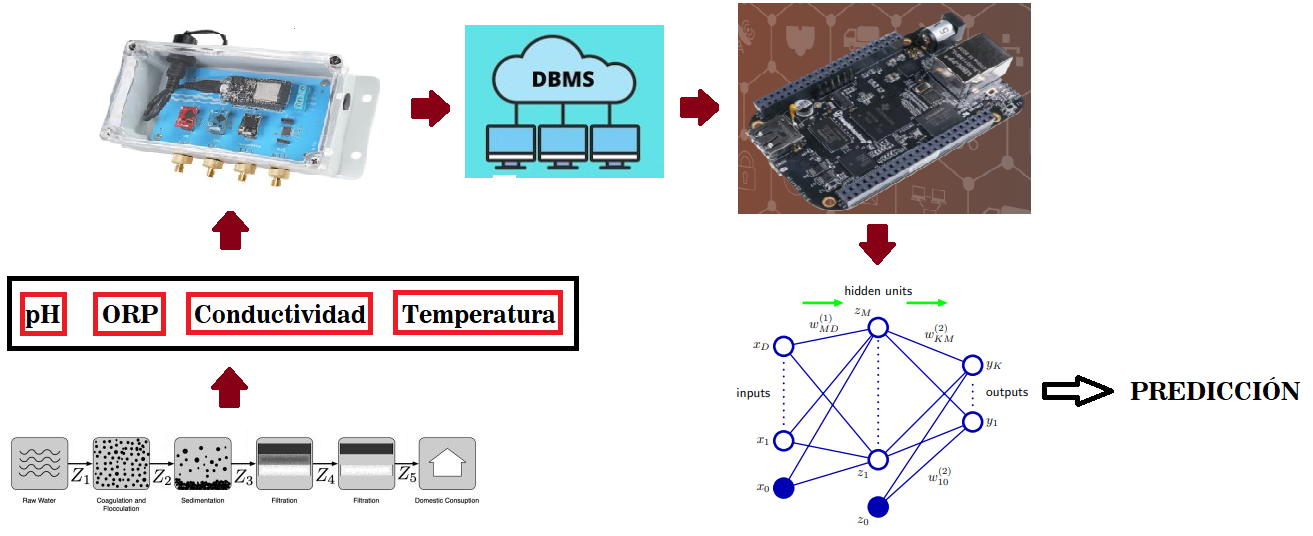
\includegraphics[scale=0.5]{figuraMetodología.png}[\centering]

%\begin{figure}[h]
	%\centering
	%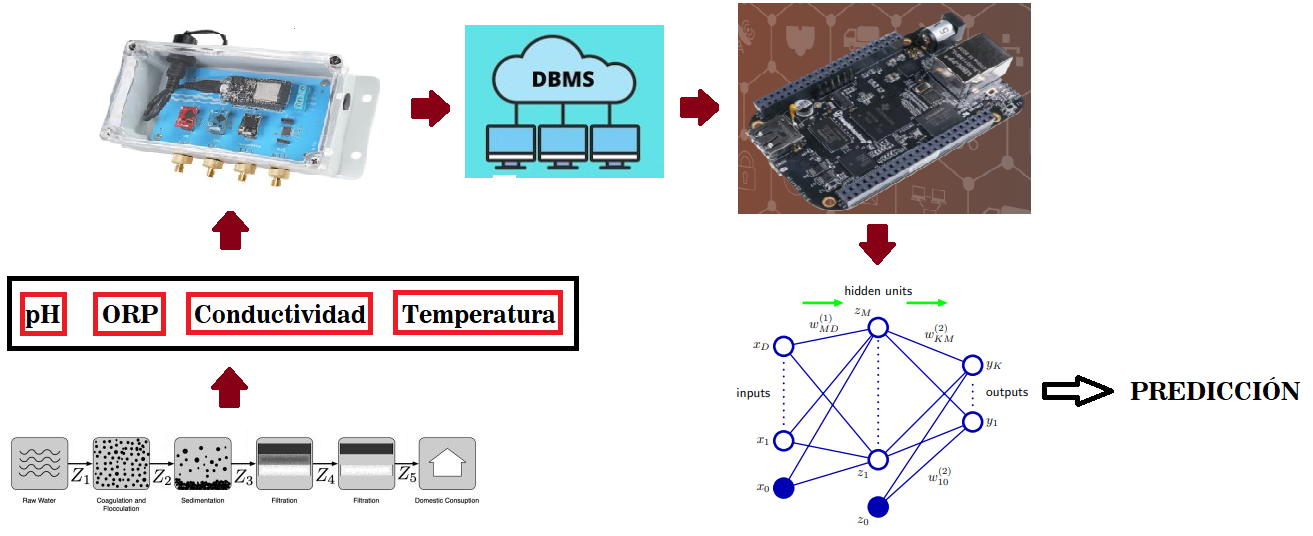
\includegraphics[scale=0.46]{figuraMetodología.png}
	%\caption{Función logística o sigmoide}
	%\label{fig:figura3_40}
%\end{figure}

%\clearpage

%\tikzstyle{startstop} = [rectangle, rounded corners, 
						%minimum width=3cm, 
						%minimum height=1cm,
						%text centered, 
						%draw=black, 
						%fill=red!30]

%\tikzstyle{io} = [trapezium, 
				  %trapezium stretches=true, % A later addition
				  %trapezium left angle=70, 
				  %trapezium right angle=110, 
				  %minimum width=3cm, 
				  %minimum height=1cm, text centered, 
				  %draw=black, fill=blue!30]

%\tikzstyle{process} = [rectangle, 
					   %minimum width=3cm, 
					   %minimum height=1cm, 
					   %text centered, 
					   %text width=3cm, 
					   %draw=black, 
					   %fill=orange!30]

%\tikzstyle{decision} = [diamond, 
						%minimum width=3cm, 
						%minimum height=1cm, 
						%text centered, 
						%draw=black, 
						%fill=green!30]
%\tikzstyle{arrow} = [thick,->,>=stealth]

%\begin{center}
%\begin{tikzpicture}[node distance=2cm]

	%\centering

	%\node (start) [startstop] {Etapas del Proceso de Potabilización};
	%\node (in1) [startstop, below of=start,yshift=-0.8cm] {pH	ORP		Conductividad		Temperatura};
	%\node (pro1) [startstop, below of=in1,yshift=-0.8cm] {Equipo WiFi Pool Kit};
	%\node (dec1) [startstop, below of=pro1, yshift=-0.8cm] {DBMS};

	%\node (pro2a) [startstop, below of=dec1, yshift=-0.8cm] {Tarjeta de desarrollo BeagleBone Black};
	
	%\node (pro2b) [process, right of=dec1, xshift=2cm] {Process 2b};
	%\node (out1) [startstop, below of=pro2a,yshift=-0.8cm] {Red Neuronal Artificial};
	%\node (stop) [startstop, below of=out1,yshift=-0.8cm] {Estimación de Calidad del Agua para una muestra};

	%\draw [arrow] (start) -- (in1);
	%\draw [arrow] (in1) -- (pro1);
	%\draw [arrow] (pro1) -- (dec1);
	%\draw [arrow] (dec1) -- node[anchor=east] {yes} (pro2a);
	%\draw [arrow] (dec1) -- node[anchor=south] {no} (pro2b);
	%\draw [arrow] (pro2b) |- (pro1);
	%\draw [arrow] (pro2a) -- (out1);
	%\draw [arrow] (out1) -- (stop);
														   
%\end{tikzpicture}
%\end{center}

%\clearpage

\begin{figure}[h]
	\centering
	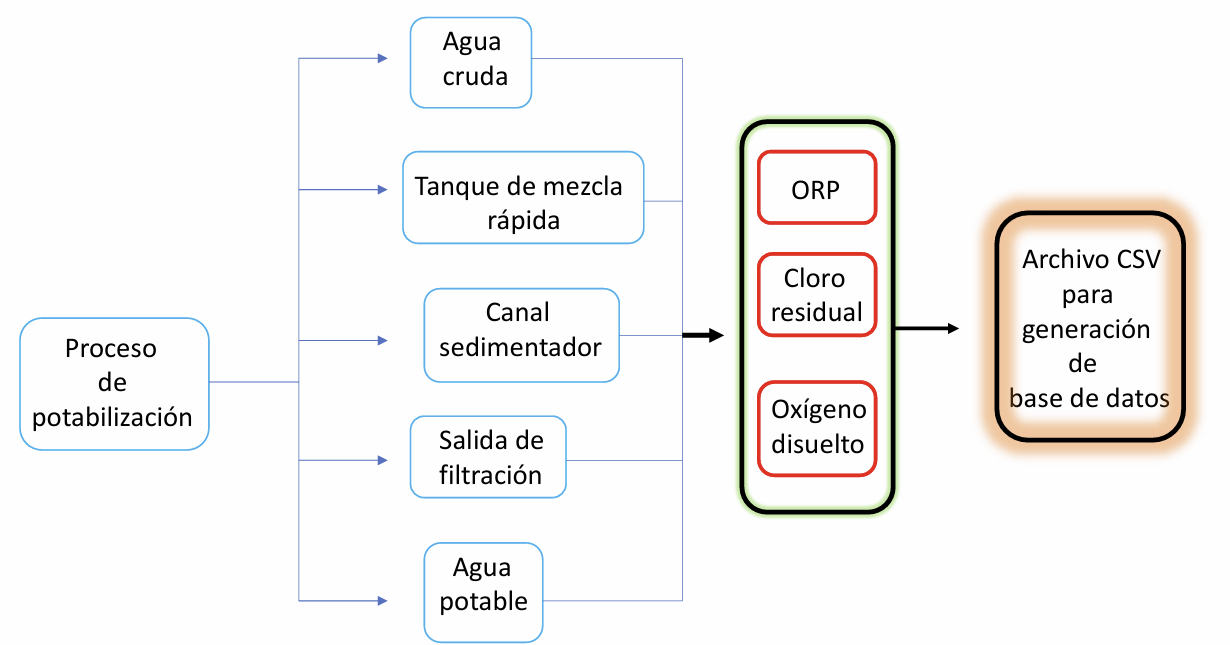
\includegraphics[scale=0.75]{imgss217.png}
	\caption{Método para generación de base de datos}
	\label{fig:figura1200_1}
\end{figure}

En el proceso de potabilización se han elegido 5 puntos específicos en los cuales se realizará la toma de muestras. Los puntos de muestreo en el proceso serán las fases de agua cruda, tanque de mezclado rápido, canal sedimentador,
la salida de filtración y finalmente el agua potable, que es el producto final del proceso de tratamiento.

Lo que se busca es lograr una caracterización del proceso mediante parámetros específicos. Por lo tanto, para cada muestra correspondiente a cada fase es necesario realizar la medición puntual o continua de los 3 parámetros 
considerados, que en este caso serán ORP, cloro residual y oxígeno disuelto. Cada vez que se realice una toma de muestras, el conjunto de mediciones registradas debe etiquetarse según la fase del proceso que corresponda, y 
gradualmente ir formando una base de datos más amplia.

En la \autoref{fig:figura1200_47} se muestra un esquema de la segunda parte para el método planteado.

\clearpage

\begin{figure}[h]
	\centering
	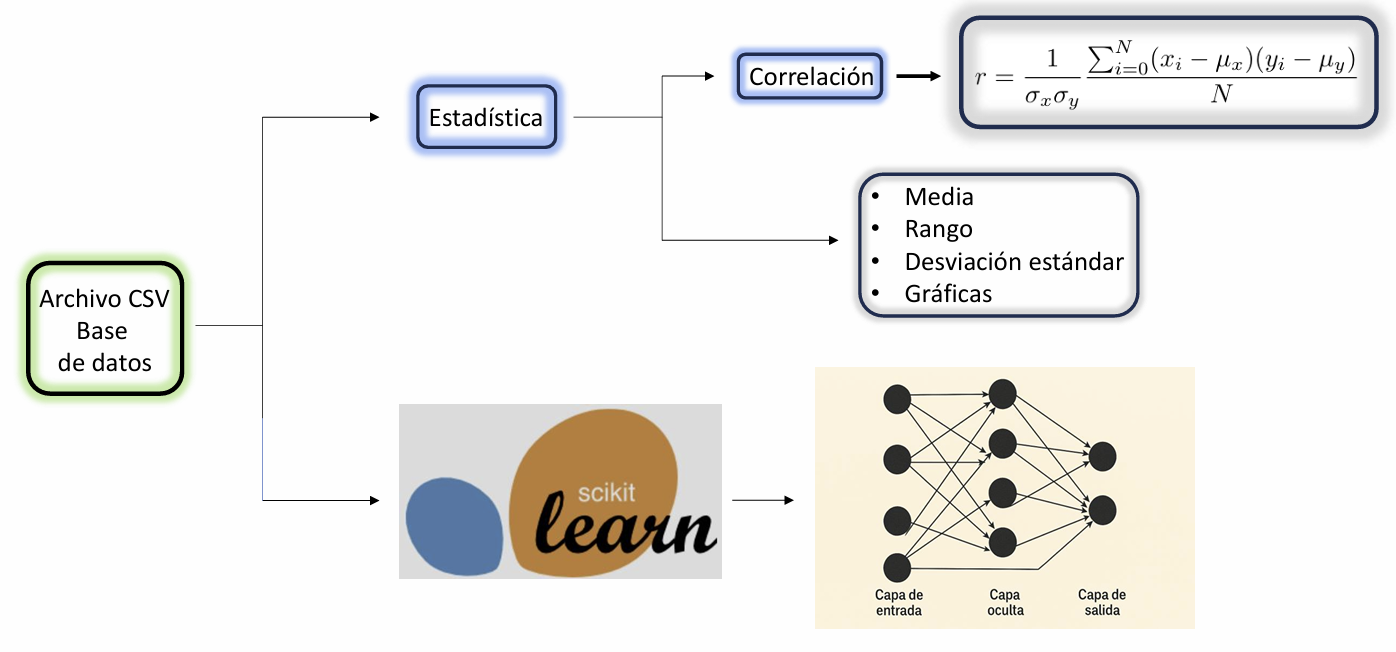
\includegraphics[scale=0.65]{imgss218.png}
	\caption{Método para tratamiento de la información}
	\label{fig:figura1200_47}
\end{figure}

Con la base de datos generada primero se realiza el análisis mediante herramientas estadísticas para conocer el comportamiento de cada parámetro medido. Se obtienen coeficientes de correlación lineal entre los 3 parámetros,
además de obtener métricas descriptivas y gráficas de los parámetros para las diferentes etapas del proceso de potabilización.

La base de datos recolectada igualmente servirá para optimizar el modelo de clasificación de calidad del agua. El conjunto de datos deberá particionarse aleatoriamente para generar grupos para entrenamiento y validación, y 
con ellos generar las pruebas necesarias hasta encontrar la mejor o mejores optimizaciones.

\clearpage

\section{Conclusiones}

En este capítulo se presenta la revisión del estado del arte en el cual se hace la exposición de trabajos teóricos acerca de los conceptos y definiciones relacionadas con la calidad del agua y los diferentes parámetros utilizados 
para su análisis. Adicionalmente, se incluyen investigaciones aplicadas en las cuales se hace uso de técnicas estadísticas y de inteligencia artificial para análisis de calidad, y dichos trabajos se pueden tomar como guía o 
referencia para el presente proyecto y así determinar que técnicas o modelos podrían adaptarse mejor a lo que nosotros realizamos.

Posteriormente, se exponen tanto los objetivos general y partículares para el proyecto con los cuales se define el propósito y alcance que se plantea para esta investigación, de acuerdo al proceso que va a estudiarse y los 
recursos con los que se trabajará. 

Finalmente, se expone el procedimiento o metodología general a seguir para lograr el alcance de los objetivos previamente establecidos. Se detalla que nuestra investigación inicia desde el conocer las características del 
proceso que se va a estar estudiando, sus diferentes parámetros y cómo se estarán midiendo para almacenar los datos monitoreados. Lo anterior con el fin de generar una base de datos que pueda caracterizar el proceso de 
potabilización y posteriormente servir para realizar estimaciones de calidad del agua mediante un modelo basado en inteligencia artificial.

\clearpage
 %Introduction
\cleardoublepage
\chapter{Regresores y Clasificadores}
\label{ch:ClasificadorRedes}

\section{Introducción}

El concepto de \textit{Inteligencia Artificial} (\textit{IA}) en los últimos años ha tomado un nivel elevado de relavancia debido a la inclusión en nuestras vidas de tecnologías que presumen de ciertas 
capacidades o características especiales. Específicamente se anuncian como tecnologías inteligentes, capaces de brindarnos apoyo en la resolución de problemas cotidianos simples y también situaciones más complejas, las 
cuales se podrían considerar posibles de resolver exclusivamente para un humano. Sin embargo, actualmente en las computadores y teléfonos inteligentes encontramos asistentes virtuales que parecieran tener un comportamiento 
lógico y racional, en las calles encontramos vehículos capaces de llevar a su dueño a su destino sin que él tenga que poner sus manos en el volante, entre muchos otros avances tecnológicos que han surgido en los últimos 
meses; y seguirán apareciendo todavía más y cada vez con mayores capacidades. Todos estos avances promocionados bajo la cualidad de funcionar mediente Inteligencia Artificial.

Para aspectos de ingeniería, la Inteligencia Artificial no es más que una rama de las Ciencias de la Computación. Desde mediados del siglo pasado, científicos del área de la computación se interesaron por la idea futurística 
y utópica de computadoras y máquinas inteligentes o independientes que pudieran realizar tareas de forma autónoma. Se desarrollaron una gran cantidad de modelos matemáticos teóricos acerca de cómo podría llegar a ser posible 
la existencia de tecnologías de ese tipo. Sin embargo, la ingeniería en general aún era inmadura como para tener la capacidad de implementar un sistema de dichas características.

Desde las primeras propuestas teóricas en las décadas de 1940 y 1950 de los cientifícos McCulloch y Pits sobre las primeras redes neuronales artificiales, que no podían pasar de ser simplemente modelos teóricos debido a la 
inexistencia de \textit{hardware} capaz de realizar ese tipo de operaciones matemáticas, hasta las actuales tarjetas \textit{GPU} (\textit{Graphics Processing Unit, Unidad de Procesamiento de Gráficos}) utilizadas en 
\textit{computación acelerada}, capaces de realizar procesamiento en paralelo y ejecutar complejas redes neuronales procesando simultáneamente millones de parámetros \cite{gpuHP} \cite{gpuNVIDIA}. Todo este proceso ha sido gradual y ha requerido del 
avance conjunto tanto de los modelos matemáticos como del hardware. Y ahora tenemos a nuestra disposición y convertidas en realidad esas ideas primitivas sobre computadoras y máquinas inteligentes.

La investigadora Elaine Rich define la IA como la rama de las Ciencias de la Computación que se encarga del estudio de cómo lograr que las computadoras sean capaces de realizar tareas que de momento un humano las puede ejecutar 
mejor \cite{ElaineRichIA}. Esta definición implica un panorama absolutamente general pero que difícilmente perdera validez con el paso de los años debido a que define de una manera muy simple pero muy certera lo que es y lo 
que se busca con el desarrollo de la IA.

De forma más específica, más allá de una definición general de IA, lo importante es conocer que aplicaciones prácticas se pueden generar con la IA, y consecuentemente qué problemas nos puede ayudar a resolver, ya sean problemas 
que aún no han sido resueltos por los humanos o que ya se pueden resolver pero la IA representa una solución más eficiente \cite{ertel}. Algunas de las aplicaciones más reconocidas de la IA se enlistan a continuación.

\begin{itemize}
    \item \textit{Computer Vision}. Se refiere al procesamiento digital de imágenes usando técnicas de IA. Los usos más comunes para este tipo de procesamiento son enfocados al reconocimiento de patrones en una imagen dada, 
    es decir, poder determinar el tipo de objetos existentes en una imagen o incluso el reconocimiento facial para la identificación de personas. 
    \item \textit{Natural Language Processing}. Refiere a Procesamiento de Lenguaje Natural. Esta área va enfocada a entrenar y automatizar sistemas computacionales para que adquieran la capacidad de reconocer y entender las 
    diversas formas de comunicación que usamos los humanos.
    \item \textit{Sistemas de Clasificación}. Son modelos matemáticos optimizados con el propósito de realizar reconocimiento de patrones dado un conjunto de datos conocidos de un conjunto de variables, con el fin de poder 
    identificar el tipo de entorno, persona u objeto que se está analizando.
    \item \textit{Neural Networks}. Refiere a Redes Neuronales. Son modelos matematicos no lineales los cuales debido a su naturaleza intrínseca de no linealidad, permiten ser útiles en un número diverso de aplicaciones.
    Permiten realizar procesamiento digital de imágenes o audio, algoritmos de clasificación, sistemas de control automático, optimización y automatización de procesos, sistemas de detección de errores, algoritmos predictivos 
    para control de procesos, modelos de regresión, entre muchas otras.   
\end{itemize}

Para la realización de este trabajo de tesis se he hecho uso principalmente de Redes Neuronales con arquitecturas específicas para que puedan funcionar como clasificador. La elección de estos modelos en específico se debe 
a la mayor complejidad de las ecuaciones matemáticas que se pueden obtener con una red neuronal, lo cual es cierto que en lo referente a cálculo computacional resulta una tarea que requiere un número mayor de operaciones, 
sin embargo, al tener ecuaciones matemáticas con mayor número de términos es posible generar patrones de clasificación mejor optimizados o ajustados a los datos reales del proceso de potabilización analizado.

En este capítulo se exponen los fundamentos matemáticos de los modelos de clasificación basados en inteligencia artificial, iniciando con las ecuaciones fundamentales para un algoritmo de regresión lineal. Después, 
se exponen las ecuaciones para el método de optimización de descenso por gradiente, el cual supone una parte importante para la implementación del modelo final de clasificación de calidad del agua que se busca desarrolllar.
Posteriormente, se explica la teoría referente a redes neuronales, pasando por la explicación sobre los parámetros importantes en la definición de su arquitectura, así como sus funciones de activación y cómo se relacionan 
con los temas previamente explicados. Finalmente, se exponen las ecuaciones matemáticas para el proceso de entrenamiento de una red neuronal, en el cual se busca ajustar el valor de los pesos sinápticos de la red mediante 
técnicas iterativas de minimización de la magnitud del error en el modelo. 

\section{Modelo de Regresión Lineal}

En Matemáticas, una \textit{regresión} tiene como objetivo estimar el valor de 1 o más variables \textit{target} continuas \textit{t}, dado un vector N-Dimensional \textit{x} de variables de entrada \cite{bishop}.

El concepto de la regresión lineal es tener un conjunto de datos de entrada y explicar o predecir las salidas como una combinación lineal de las variables o datos de entrada. Es decir, lograr obtener una ecuación lineal 
optimizada que genere la mejor explicación o descripción posible de los datos de entrada. Se busca encontrar la relación entre las variables independientes y dependientes mediente el mejor ajuste posible de una línea recta 
con los puntos que representan los datos de entrada. Este lugar geométrico buscado se conoce como \textit{línea o plano de regresión} \cite{BigDataCandel}.

El modelo general de regresión lineal tiene la forma (\ref{eq:ecuacion701}).

\begin{equation}
	y(x,w)=w_0+w_1x_1+ \cdot \cdot \cdot +w_Dx_D
	\label{eq:ecuacion701}
\end{equation}

Es decir, \textit{y} es la variable target que se busca predecir mediante una combinación lineal de un número \textit{D} de variables de entrada. 

La \autoref{fig:figura700_1} muestra un ejemplo básico en 2 dimensiones.

\begin{figure}[h]
	\centering
	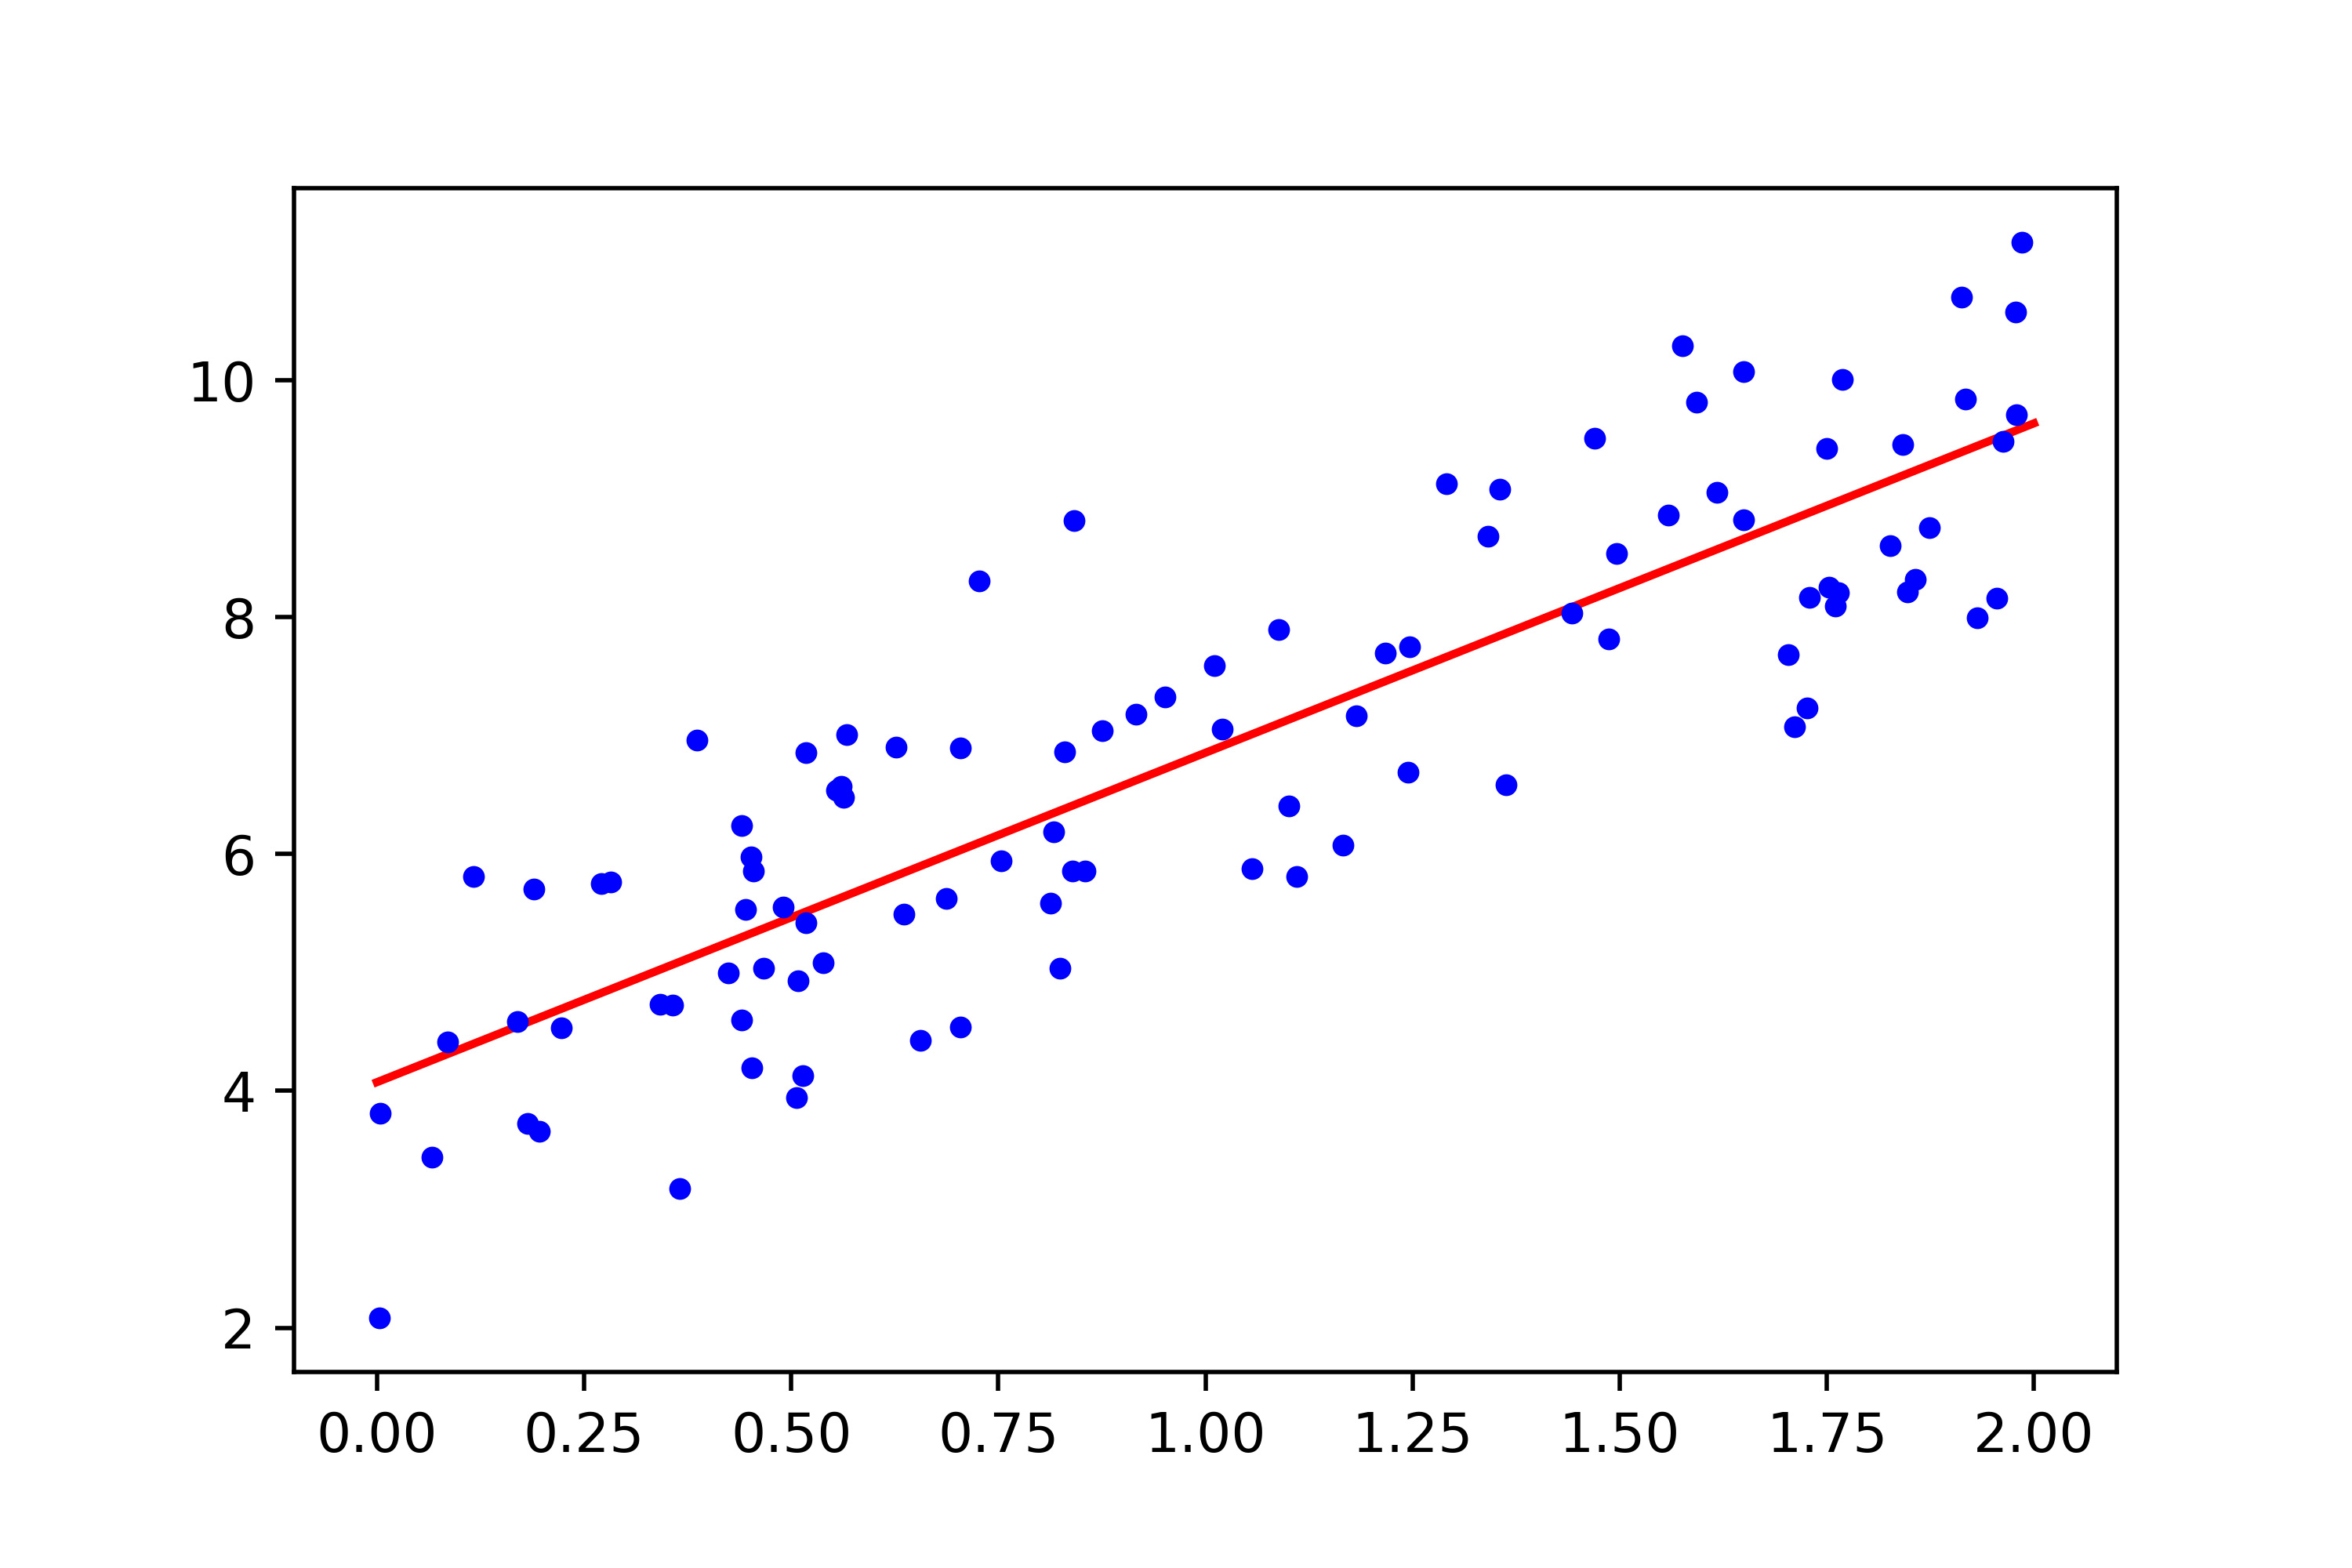
\includegraphics[scale=0.7]{imgss144.png}
	\caption{Aproximación de un conjunto de datos usando una línea de regresión}
	\label{fig:figura700_1}
\end{figure}

En la \autoref{fig:figura700_1} se tiene un diagrama de dispersión con los puntos o datos de 2 variables cualesquiera. Supongamos que se busca una función matemática que pueda tener este mismo comportamiento generado por 
estos datos. Si se quisiera tener una ecuación que igualara de forma perfecta esta tendencia y el lugar geométrico trazado cruzara por todos los puntos, probablemente habría que recurrir a un ejercicio de interpolación 
polinómica, pero esto implicaria generar un polinomio complejo de grado superior.  

Si no es necesario replicar de manera perfecta el comportamiento mostrado por los puntos graficados, y resulta suficiente con generar una expresión matemática que siga la misma tendencia sin necesidad de cruzar por cada 
uno de los puntos de la gráfica, entonces se puede recurrir a un ejercicio de regresión lineal que pueda generar una función matemática cuyo lugar geométrico generado sea una recta en 2 dimensiones, tal y como se muestra 
en la \autoref{fig:figura700_1}. Para este ejemplo mostrado, se observa que la recta de color rojo trazada no cruza por casi ninguno de los puntos, sin embargo, logra replicar la tendencia del comportamiento de una forma 
general.

El objetivo de este método es hallar los valores óptimos del vector de pesos \textbf{w}, dado de la forma (\ref{eq:ecuacion702}).

\begin{equation}
	\textbf{w}=(w_0,w_1,...,w_D)
	\label{eq:ecuacion702}
\end{equation}

\subsection{Método de Mínimos Cuadrados para la Regresión Lineal}

Una vez que se tiene la forma descriptiva de los datos de las variables para las cuales se busca una aproximación mediante regresión lineal, lo que sigue es encontrar una ecuación lineal que permita representar la mayor 
cantidad de puntos dados por los datos de entrada. Se busca que dicha ecuación lineal pase lo más cerca posible por cada uno de los puntos, para lo cual es necesario optimizar los valores de los coeficientes o pesos de la 
combinación lineal. El método de \textit{Mínimos Cuadrados} permite dar un paso a una posible solución para dicha optimización de los coeficientes de la combinación.

La idea del método de mínimos cuadrados consiste en calcular la diferencia entre las predicciones hechas por el modelo de regresión y los valores reales de la variable \textit{target}. Dado que el valor del \textit{error} 
arrojado por estas diferencias puede generar números negativos, dichas diferencias deben ser elevadas al cuadrado para posteriormente realizar la sumatoria de todos estos valores de error, y finalmente el valor de dicha 
suma dividirlo entre el valor total de muestras del conjunto de datos. A este último resultado se le conoce como \textit{error cuadrático medio} (\textit{MSE, Mean Square Error}), y entre menor sea su valor, mejor será el 
ajuste realizado para los pesos del modelo \cite{PinedaPertuzML}.

El error cuadrático medio (MSE) se define de la forma (\ref{eq:ecuacion703}).

\begin{equation}
	MSE=\frac{1}{m} \sum_{i=1}^{m}e_s
	\label{eq:ecuacion703}
\end{equation}

donde $e_s$ se define de la forma (\ref{eq:ecuacion704}).

\begin{equation}
	e_s=(y_{pred} - t)^2
	\label{eq:ecuacion704}
\end{equation}

Es decir, el cuadrado de la diferencia de el valor predicho y el valor target deseado.

\subsection{Descenso por Gradiente}

El método de \textit{descenso por gradiente} es un algoritmo iterativo usado en regresión lineal para encontrar el valor óptimo de los pesos de la combinación lineal que minimicen una \textit{función de costo}. Para cada 
iteración que se ejecuta este algoritmo, se realiza una actualización en el valor de los pesos \cite{PinedaPertuzML}. Para ilustrar cómo es que opera este método se usa como apoyo la \autoref{fig:figura700_2}.

\begin{figure}[h]
	\centering
	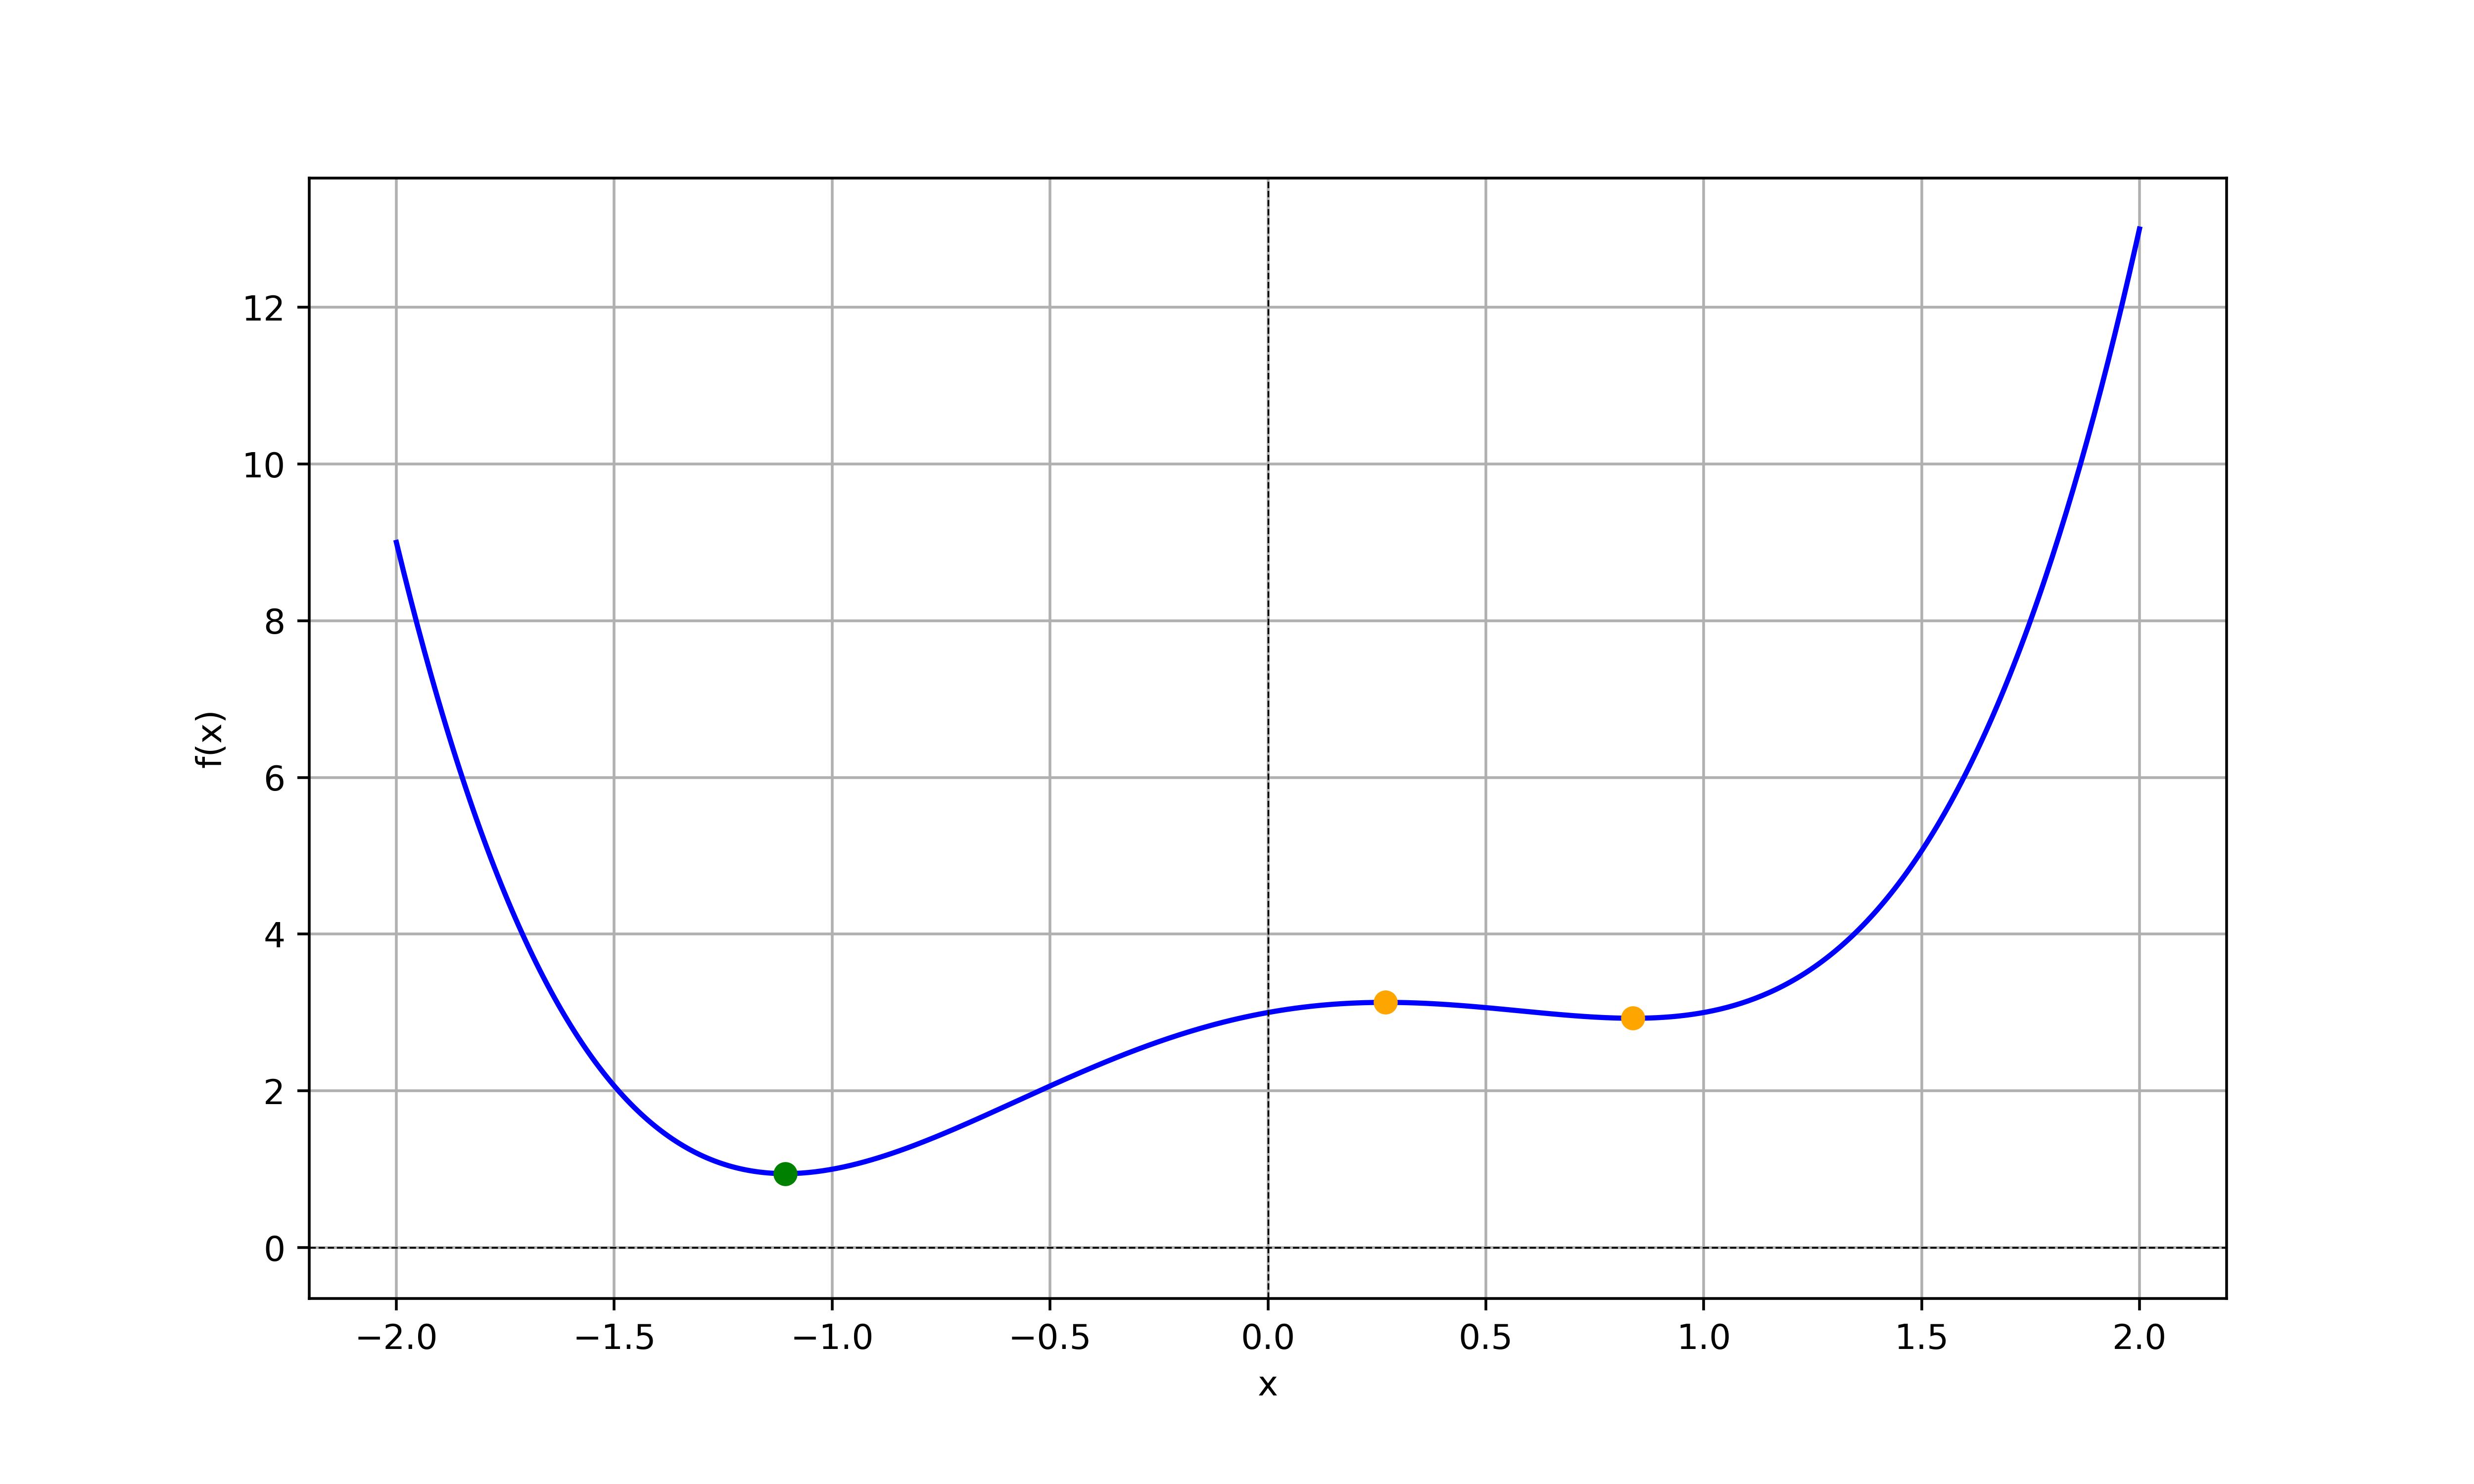
\includegraphics[scale=0.6]{imgss206.png}
	\caption{Ejemplo de una función de costo}
	\label{fig:figura700_2}
\end{figure}

De forma simple, una función de costo es una expresión matemática que nos indica el MSE, y para esta función lo que se busca es encontrar su \textit{mínimo global}. Es decir, el valor más pequeño que puede tomar la variable 
dependiente de la función. Tomando como ejemplo la \autoref{fig:figura700_2}, donde se grafica una hipotética función de costo, la idea de este método es encontrar el valor de \textit{x}  que genere el valor 
más pequeño de la función \textit{f(x)}. Con esto, teniendo que \textit{x} representa un peso y \textit{f(x)} representa el MSE, lo que se está logrando es encontrar el valor del peso que genera la máxima 
minimización del error para la regresión lineal.

Por lo tanto, una función de costo se define de la forma (\ref{eq:ecuacion705}).

\begin{equation}
	J(\textbf{w})=\frac{1}{m} \sum_{i=1}^{m}e_s
	\label{eq:ecuacion705}
\end{equation}

Donde $e_s$ tiene la forma (\ref{eq:ecuacion706}).

\begin{equation}
	e_s=(y_{pred} - t)^2
	\label{eq:ecuacion706}
\end{equation}

Es decir, las mismas ecuaciones que para el MSE.

Para este tema, es necesario realizar la definición de la herramienta matemática que nos ayuda a hacer posible este método de optimización.

El \textit{gradiente} de una función \textit{f} de \textit{n} variables se define de la forma (\ref{eq:ecuacion707}) \cite{CalculoVectorialLarson}.

\begin{equation}
	\nabla{f} (x_1,x_2,...,x_n)= \hat{x_1} \frac{\partial{f}}{\partial{x_1}} +\hat{x_2} \frac{\partial{f}}{\partial{x_2}} + ... + \hat{x_n} \frac{\partial{f}}{\partial{x_n}} 
	\label{eq:ecuacion707}
\end{equation}

Es decir, el gradiente de una función genera como resultado un campo vectorial, en donde cada uno de los términos es el producto de la derivada parcial de la función respecto a una de las variables independientes con su 
correspondiente vector unitario. 

La importancia de este resultado para la optimización de los pesos en la regresión lineal radica en la interpretación o efecto geométrico que pueden tener este campo vectorial evaluado en un punto cualquiera permitido para 
las variables independientes.

Un análisis a fondo de este campo vectorial del gradiente, arroja como resultado que dicho campo vectorial evaluado en un punto, ese vector resultante representa para ese punto la dirección y sentido del \textit{máximo incremento o ascenso} 
para la función \textit{f} \cite{CalculoVectorialDennisZill}. Es decir, el gradiente de la función evaluado en un punto nos indica la dirección a donde tendríamos que movernos si quisiéramos ascender de la manera más rápida
sobre la superficie n-dimensional dada por la función \textit{f}.

Podemos hacer una comparación de la función de costo \textit{J(w)} con la función \textit{f} a la cual se le aplica el gradiente. El gradiente nos permite encontrar la forma más rápida de ascender sobre la función que se 
está analizando, pero en la función de costo para la regresión lineal lo que se busca es llegar al punto más bajo, el ya mencionado mínimo global. Si el gradiente nos entrega la forma más rápida de ascender, entonces la 
forma más rápida para descender sobre la función de costo nos la entregaría el inverso aditivo del gradiente aplicado a la función de costo (\ref{eq:ecuacion708}).

\begin{equation}
	- \nabla{J(w)}= - \hat{w_1} \frac{\partial{J(w)}}{\partial{w_1}} - \hat{w_2} \frac{\partial{J(w)}}{\partial{w_2}} - ... - \hat{w_n} \frac{\partial{J(w)}}{\partial{w_n}} 
	\label{eq:ecuacion708}
\end{equation}

Es aquí con este resultado que encontramos cómo podemos generar el método de descenso por gradiente para la regresión lineal. En cada una de la iteraciones del algoritmo, se puede realizar una actualización de los pesos o 
coeficientes al dar pequeños \textit{pasos} en la dirección opuesta dada por el vector gradiente. El ejemplo clásico para este caso es imaginar el estar en la cima de una montaña y se desea descender hasta el punto más 
bajo de la misma, pero que el descenso sea de la forma más adecuada u óptima posible; cuando se está en las partes altas de la montaña, donde la pendiente es elevada, el descenso se puede hacer de forma más rápida al dar 
\textit{pasos más grandes}; caso contrario, cuando se está en puntos más bajos de la montaña donde la pendiente es menor, se tendrá que dar \textit{pasos más pequeños} \cite{PinedaPertuzML}.

Ahora supongamos que se tiene el vector de pesos de la forma (\ref{eq:ecuacion702}); iterativamente se desea encontrar sus valores que generen que la función de costo \textit{converga} hasta un valor mínimo o que se halla 
cumplido un valor umbral establecido previamente para el MSE. La ecuación (\ref{eq:ecuacion709}) expresa la modificación necesaria para el d-ésimo peso en cada iteración del algoritmo.

\begin{equation}
	w_D = w_D - \alpha \frac{\partial{J(w)}}{\partial{w_D}}
	\label{eq:ecuacion709}
\end{equation}

En la ecuación (\ref{eq:ecuacion709}) el factor $\alpha$ se denomina la \textit{tasa de aprendizaje} del algoritmo. Este factor representa el \textit{tamaño de los pasos} dados en el descenso para cada iteración.
Es decir, sirve para controlar cuánto se \textit{avanza} y se suele asignársele un valor en el rango de 0.0001 a 1, aunque a veces se suele asignar valores cercanos a 10 y el algoritmo funciona de mejor forma que para 
otros valores. La asignación de su valor se hace mediente prueba y error, considerando que un valor muy grande puede ocasionar que se produzcan \textit{saltos bruscos} de un lado a otro sobre la superficie de error \textit{J(w)},
provocando que el valor del error MSE se incremente y decremente continuamente y el algoritmo nunca alcance la convergencia. De la misma forma, un valor demasiado pequeño puede ocasinar que el algoritmo requiera un número 
muy elevado de iteraciones, lo cual en muchas ocasiones es un problema a nivel de cálculo computacional \cite{PinedaPertuzML}.

El proceso de iteraciones del algoritmo de descenso por gradiente se repite hasta que el valor del error MSE sea un valor muy pequeño cercano a 0; dado que es muy poco probable alcanzar el valor de 0 para el MSE, el 
algoritmo se suele controlar asignando un número límite de \textit{épocas} o iteraciones que logre generar un valor de MSE lo suficientemente bajo para los requisitos dados por la aplicación dada.

Para el caso de estudio de algoritmos de clasificación basados en redes neuronales, la optimización para minimización del error por descenso por gradiente será en nuestro caso el método empleado. Para el problema que se 
analiza en este proyecto, existen métodos de optimización más complejos, sin embargo el método de descenso por gradiente resulta suficiente y adecuado gracias a su eficiencia en casos donde se emplea una gran cantidad de 
datos para entrenamiento del modelo, lo que permite al mismo tiempo reducir la carga computacional. Adicionalmente, este método resulta adecuado en problemas donde no es necesario obtener una solución exacta, como en el 
caso de una red neuronal que se busca principalmente la mejor optimización posible.

\section{Modelos no Lineales para Clasificación}

En IA, un algoritmo de clasificación consiste en tomar un conjunto de características \textbf{x} de un objeto, proceso o ente, y dicho valor asignarlo a 1 de \textit{K} valores posibles \cite{bishop}. Es decir, por ejemplo, 
existen diferentes tipos de calzado dependiendo del uso que tendrá, consecuentemente cada clase diferente de calzado tendrá diferentes caracteristicas.

En los problemas de clasificación existen diversas maneras de usar los valores \textit{target} para poder representar las \textit{etiquetas} de clase, es decir, las diferentes clases o tipos que se manejan en un problema 
dado. Por ejemplo, en modelos probabilísticos, para el caso de únicamente 2 clases posibles, la forma más común es usar 1 sola variable target \textit{t} que tome 2 valores solamente, 0 y 1. De esta forma \textit{t=1} representa la clase \textit{$C_1$} y \textit{t=0} representará a la clase restante \textit{$C_2$}.
Un problema de este tipo se conoce como \textit{clasificación binaria} y un ejemplo simple sería la diferenciación en el sexo o genero de una persona, que puede tomar 2 clases posibles, hombre o mujer.

Para un valor de \textit{K} mayor a 2 clases posibles, \textit{clasificación multiclase}, es conveniente usar una variable \textit{t} que sea un vector de tamaño \textit{K}, de forma que si el clasificador arroja como resultado correcto la clase \textit{$C_j$}, 
entonces todos los elementos \textit{$t_k$} de \textbf{t} sean 0 y el elemento \textit{$t_j$} se le asigne un valor de 1 \cite{bishop}. Un ejemplo sería dado por (\ref{eq:ecuacion710}).

\begin{equation}
	\textbf{t}=(0,1,0,0,0)
	\label{eq:ecuacion710}
\end{equation}

%La ecuación (\ref{eq:ecuacion710}) podría representar un ejemplo de clasificación con 5 clases posibles, en el cual un vector de entrada específico entrega como resultado que la clase \textit{$C_2$} es la correcta para el 
%vector de entrada dado.

La ecuación (\ref{eq:ecuacion710}) podría representar un ejemplo de resultado de un algoritmo de clasificación con 5 clases posibles, en el cual el segundo elemento del vector correspondiente a la clase \textit{$C_2$} tiene 
un valor de 1 y los demás elementos del vector son 0, indicando que esa es la estimación del clasificador. Un ejemplo sería el caso de un modelo clasificador que analice imágenes de playeras y las clasifique de acuerdo a 
sus características; por ejemplo, playeras deportivas, playeras para eventos formales, playeras de tipo casual, playeras de pijama y playeras para entornos laborales. El clasificador analizaría las imágenes para determinar 
las características físicas y poder estimar el tipo de playera que se encuentra en la imagen.

Para tareas de clasificación, los modelos matemáticos usados en regresión lineal pueden ser de utilidad para generar nuevos algoritmos para generar los clasificadores. Para lograr esto, se puede establecer una generalización 
de los modelos para regresión al usar una función no lineal sobre la función lineal aplicada a los pesos o coeficientes del modelo (\ref{eq:ecuacion711}) \cite{bishop}.

\begin{equation}
	y(\textbf{x})=f(\textbf{w}_{transpose} \textbf{x} + w_0)
	\label{eq:ecuacion711}
\end{equation}

En modelos de clasificación, la función \textit{f} se conoce como \textit{función de activación}. 

\subsection{Regresión Logística}

La \textit{regresión logística} es un modelo de clasificación usado tanto para clasificación binaria (únicamente 2 clases posibles) como clasificación multiclase (más de 2 clases posibles). Su aplicación se basa en el uso 
de una función matemática conocida \textit{sigmoide}, cuya definición se muestra en (\ref{eq:ecuacion712}), y en la \autoref{fig:figura700_3} se muestra su gráfica.

\begin{equation}
	f(x)=\frac{1}{1+exp(-x)}
	\label{eq:ecuacion712}
\end{equation}

\begin{figure}[h]
	\centering
	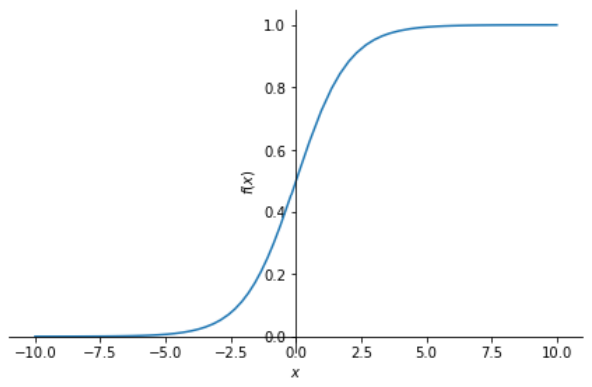
\includegraphics[scale=1]{correcionImgss40.png}
	\caption{Función logística o sigmoide}
	\label{fig:figura700_3}
\end{figure}

Esta función matemática con forma de \textit{S estilizada} presenta un comportamiento asintótico en los valores de 0 y 1, teniendo dicha tendencia para el valor de \textit{f(x)=0} cuando su argumento \textit{x} es negativo, 
y la misma tendencia para \textit{f(x)=1} cuando el argumento es positivo.

%Para esta función su uso convencional está dado por el uso de \textit{$\sigma$}.

A partir de la teoría de modelos probabilísticos para un problema de 2 clases, se sabe que la probabilidad de una clase $C_1$ dado un conjunto de valores de entrada \textbf{x} puede expresarse de la forma (\ref{eq:ecuacion713}) \cite{bishop}.

\begin{equation}
	p(C_1 | \textbf{x})=\sigma ((w)^T \textbf{x})
	\label{eq:ecuacion713}
\end{equation}

Por lo tanto, para la clase restante se tiene (\ref{eq:ecuacion714}).

\begin{equation}
	p(C_2 | \textbf{x})=1-p(C_1 | \textbf{x})
	\label{eq:ecuacion714}
\end{equation}

Las ecuaciones (\ref{eq:ecuacion713}) y (\ref{eq:ecuacion714}) constituyen el modelo de \textit{regresión logística} para clasificación. Para poder ajustar los pesos del modelo mediante técnicas de descenso por gradiente, 
primero se define lo que se conoce como \textit{función de verosimilitud} para la regresión logística (\ref{eq:ecuacion715}), la cual describe la probabilidad de un conjunto de targets dado un cierto valor en los pesos del modelo \cite{bishop}.

\begin{equation}
	p(\textbf{t} | \textbf{w})=\prod_{n=1}^{N} (y_n)^{t_n} (1-y_n)^{1-t_n}
	\label{eq:ecuacion715}
\end{equation}

donde el factor $y_n$ es la probabilidad de una de las clases dado un vector de características de entrada para el clasificador.

A partir de (\ref{eq:ecuacion715}), se puede definir una \textit{función de error} para la regresión logística. Para esto, se debe aplicar el inverso aditivo del logaritmo natural a la función de verosimilitud (\ref{eq:ecuacion716}) \cite{bishop}.

\begin{equation}
	E(\textbf{w})= -ln (p(\textbf{t} | \textbf{w}))  =- \sum_{n=1}^{N} {t_n ln(y_n) + (1 - t_n) ln (1-y_n)}
	\label{eq:ecuacion716}
\end{equation}

Al tomar el gradiente de la función en (\ref{eq:ecuacion716}) con respecto al vector de pesos, se tiene (\ref{eq:ecuacion717}) \cite{bishop}.

\begin{equation}
	\nabla{E(\textbf{w})}= \sum_{n=1}^{N} {(y_n - t_n) x_n}
	\label{eq:ecuacion717}
\end{equation}

Es decir, para este caso particular el gradiente de la fu{nción de costo del algoritmo depende del error del modelo, es decir, la diferencia del valor predicho y el valor real, además del vector de características o datos 
de entrada. Una vez que se tiene el resultado (\ref{eq:ecuacion717}), con él se puede avanzar con el método iterativo para actualizar el vector de pesos del modelo tomando como referencia la información que entrega el 
gradiente de la función de costo. El método para este caso se basa en el algoritmo de \textit{optimización iterativa de Newton-Raphson}, el cual trabaja con aproximaciones cuadráticas para la función de verosimilitud \cite{bishop}. El 
algoritmo de actualización de Newton-Raphson para minimizar una función de costo toma la forma (\ref{eq:ecuacion718}).

\begin{equation}
	{\textbf{w}}_{new}= {\textbf{w}}_{old} -{(\textbf{H})^{-1}} \nabla{E(\textbf{w})}
	\label{eq:ecuacion718}
\end{equation}

donde \textbf{H} es la \textit{matriz Hessiana}, la cual se forma con las segundas derivadas de la función de costo con respecto a las componentes del vector de pesos \textbf{w}, dada por (\ref{eq:ecuacion719}).

\begin{equation}
	\textbf{H}= \nabla{\nabla{E(\textbf{w})}}
	\label{eq:ecuacion719}
\end{equation}

Por lo tanto, la ecuación para la actualización iterativa de los pesos del modelo de regresión logística queda de la forma (\ref{eq:ecuacion720}).

\begin{equation}
	{\textbf{w}}_{new}= {\textbf{w}}_{old} -{(\nabla{\nabla{E(\textbf{w})}})^{-1}} \nabla{E(\textbf{w})}
	\label{eq:ecuacion720}
\end{equation}

El método de regresión logística al tener un enfoque probabilístico, de manera general los resultados entregados por la función sigmoide para un conjunto de pesos y valores de entrada específicos, son valores que representan 
las probabilidades para cada una de las clases involucradas. Es decir, al evaluar el modelo se tienen como resultados valores entre 0 y 1 para cada clase individual, indicando estos la probabilidad correspondiente a cada 
clase de ser la estimación correcta. Igualmente, la suma de los valores dados como resultado debe ser 1, y la estimación para el modelo suele determinarse tomando como referencia el resultado de magnitud mayor, entendiéndose 
que la clase correspondiente a dicho resultado es la estimación dada por este método.

\section{Redes Neuronales Artificiales}

\subsection{La Neurona Biológica}

El concepto o idea de Neurona fue introducido a finales del siglo XIX por el científico español Santiago Ramón y Cajal. En sus investigaciones planteó que el sistema nervioso del cuerpo humano estaba compuesto por neuronas 
individuales, las cuales se comunicaban entre sí por medio de interacciones a las que denominó \textit{sinápsis} \cite{caicedoANN}. Actualmente, gracias al desarrollo de la neurobiología sabemos que este planteamiento es 
válido.

Básicamente, una neurona es un tipo de célula biológica. Su forma esférica varía entre 5 a 10 micras de diámetro, y de ella emanan una rama principal denominada \textit{axón}, además de otras ramas de longitud más corta 
denominadas \textit{dendritas} \cite{caicedoANN}. En la \autoref{fig:figura700_4} se muestra una ilustración de la estructura de una neurona biológica.

\begin{figure}[h]
	\centering
	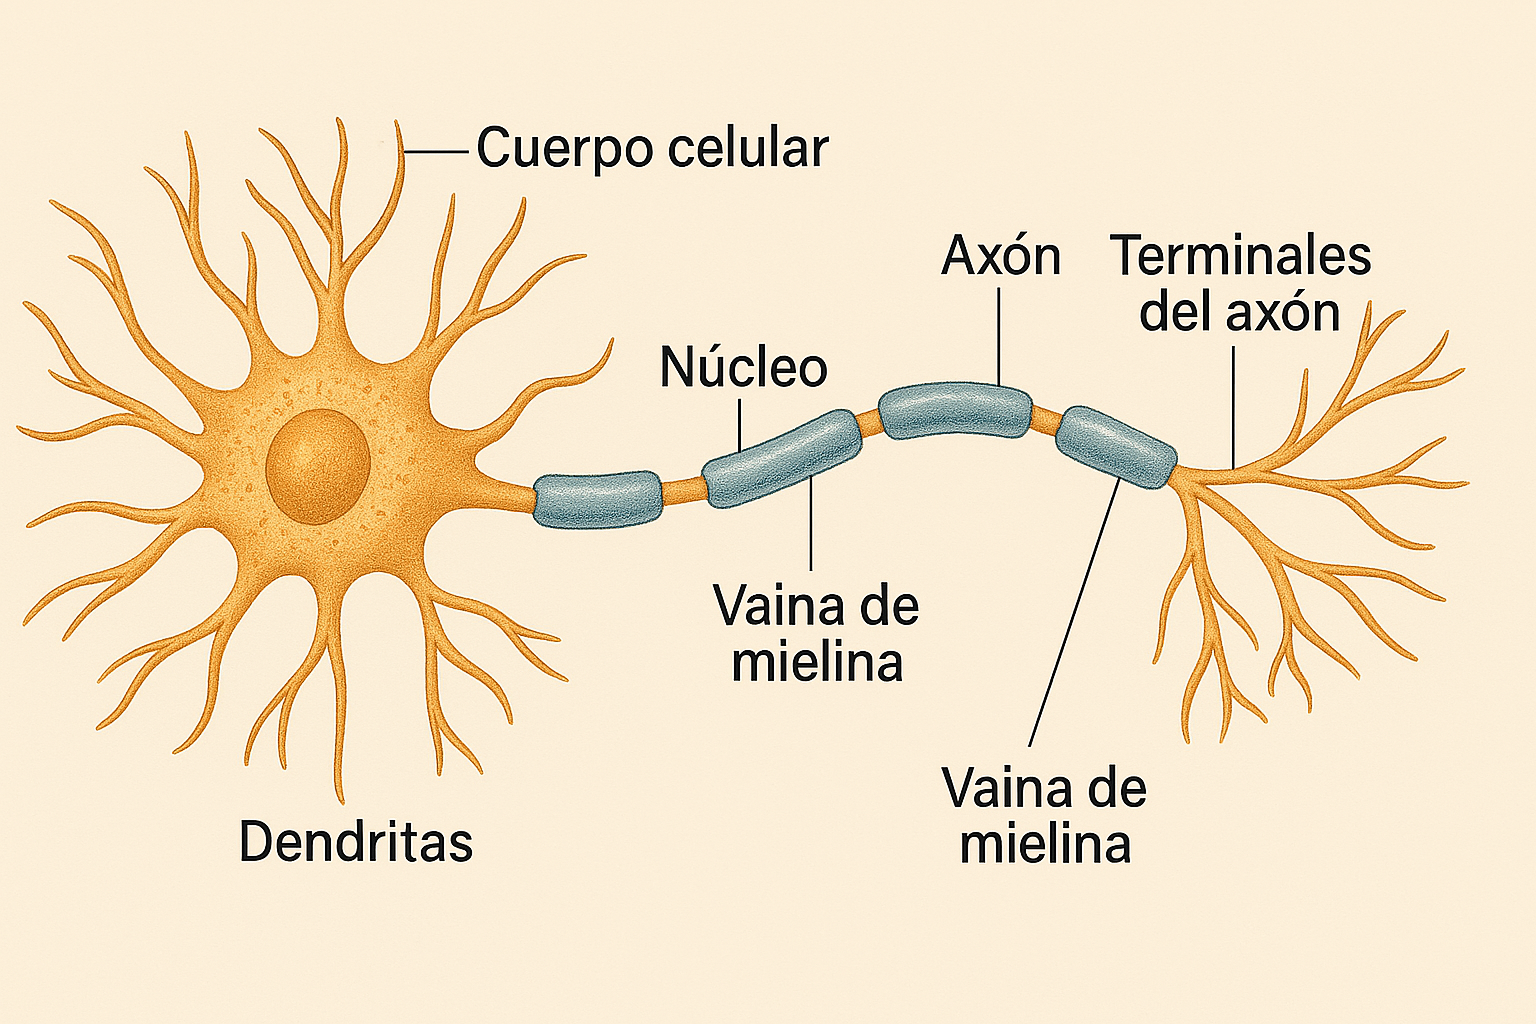
\includegraphics[scale=0.2]{imgss214.png}
	\caption{Estructura básica de una neurona biológica. Imagen generada con recursos de Internet}
	\label{fig:figura700_4}
\end{figure}

Una de las características que diferencian a las neuronas de otros tipos de células biológicas, es la capacidad que tienen para comunicarse. Este proceso de comunicación consiste en que las dendritas y el cuerpo de la neurona 
reciben señales de entrada, las cuales el cuerpo de la neurona las combina y posteriormente se emiten señales de salida a través de la terminal del axón, el cual se encarga de transmitir dicha salida a un nuevo conjunto de
neuronas. Generalmente, una neurona recibe información de miles de otras neuronas y envía información a miles de otras más \cite{caicedoANN}.

En una neurona, las señales existentes puedes ser de naturaleza química o eléctrica; la señal generada por la neurona y transportada mediante el axón es una señal eléctrica, mientras que la señal que se transmite entre la 
terminal del axón y las dendritas de otras neuronas es una señal de naturaleza química. La comunicación entre neuronas no se realiza mediante contacto directo, se lleva a cabo a través del fenómeno denominado \textit{sinápsis}.
La sinápsis es un espacio que está ocupado por unas sustancias químicas llamadas neurotransmisores, los cuales se encargan de bloquear o dejar pasar las señales que provienen de otras neuronas. En este punto, una neurona 
dada va recibiendo las señales provenientes de otras neuronas con las que tenga comunicación, y dichas señales se acumulan para posteriormente definir qué hacer \cite{caicedoANN}.

Cuando se tiene la acumulación de un conjunto de señales, si la \textit{suma} de todas ellas es lo suficientemente grande, se puede vencer el \textit{potencial de acción}, lo que permite que la neurona se active o por el 
contrario permanezca inactiva. Si la neurona es capaz de activarse, entonces tiene la capacidad de transmitir un impulso eléctrico a las neuronas con las cuales tiene comunicación, las cuales reciben dicho impulso como una 
entrada \cite{caicedoANN}.

\subsection{Aproximación Matemática Para Un Modelo De Neurona Artificial}

La \autoref{fig:figura700_5} muestra un dibujo para explicar el proceso de cómo sería una formulación matemática para llevar la neurona biológica a un modelo matemático que después pueda ser de utilidad para las Redes Neuronales 
Artificiales. Comúnmente este modelo se le denomina \textit{perceptrón}.

\begin{figure}[h]
	\centering
	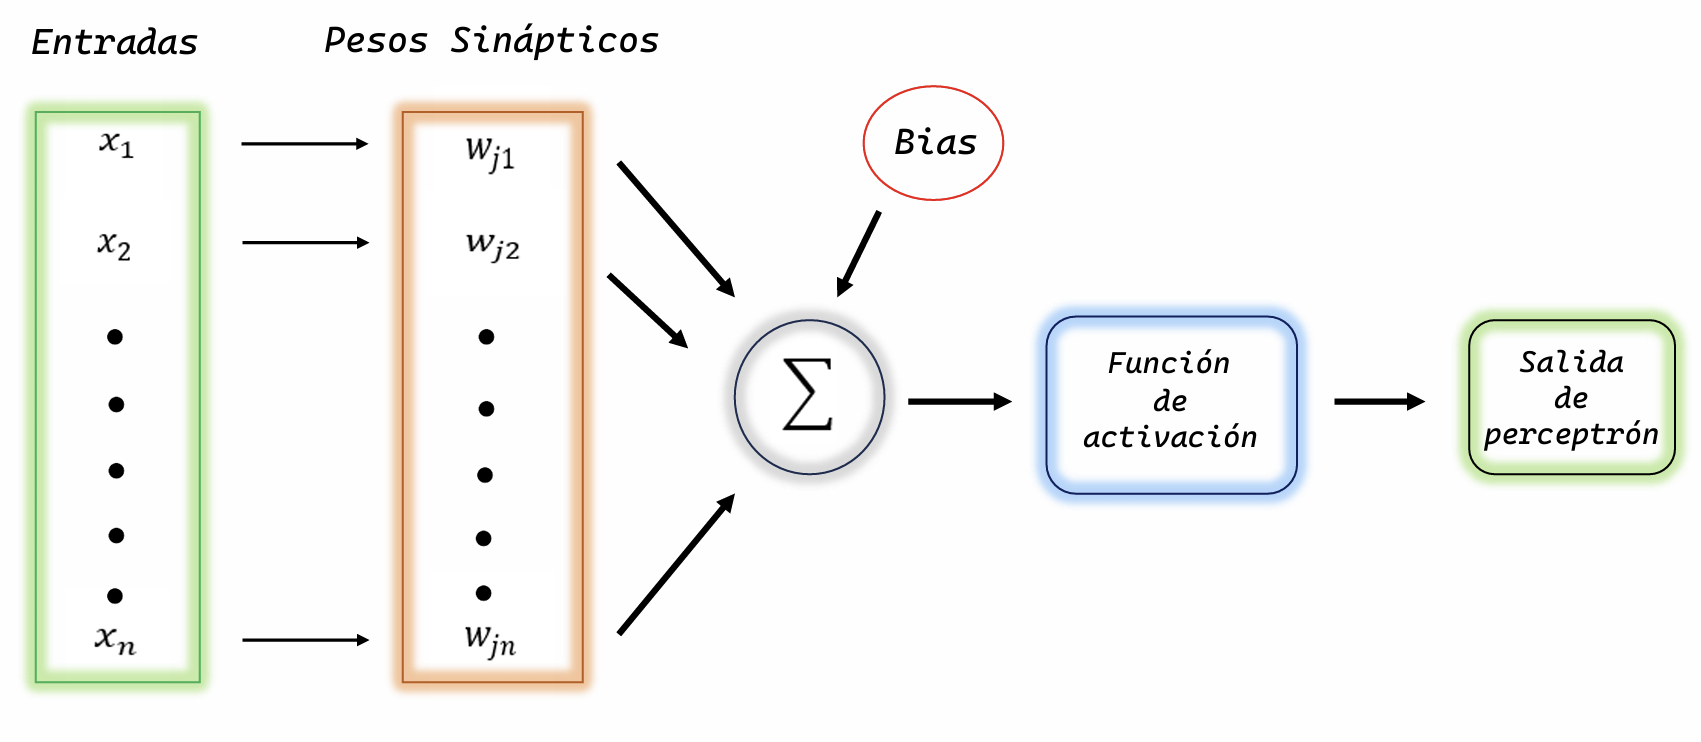
\includegraphics[scale=0.55]{imgss219.png}
	\caption{Modelo de perceptrón}
	\label{fig:figura700_5}
\end{figure}

Al igual que una neurona biológica, para el modelo de perceptrón también se tienen las entradas receptoras de señales provenientes de otras neuronas con las cuales hay conexión para transmisión de información \cite{caicedoANN}. 
Para el modelo planteado en la \autoref{fig:figura700_5}, el vector de entradas \textbf{X} toma la forma (\ref{eq:ecuacion721}).

\begin{equation}
	\textbf{X}= (x_1, x_2, ... , x_n)
	\label{eq:ecuacion721}
\end{equation}

La información recibida en la neurona es modificada por un vector de \textit{pesos sinápticos} \textbf{W}, cuyo papel es emular la sinápsis existente entre las neuronas biológicas. Estos valores de pesos sinápticos se pueden 
interpretar como una \textit{ganancia en la señal}, es decir, amplificar o atenuar los valores de entrada. Adicionalmente, se coloca un término constante conocido como \textit{bias o sesgo}, cuya función es agregar una señal 
adicional a la \textit{función de activación} con el propósito de eliminar la linealidad del modelo provocada cuando las entradas son iguales a 0 \cite{caicedoANN}.

Los diferentes valores que recibe la neurona a las entradas, modificados por los pesos, son sumados para generar el resultado \textit{entrada neta}, la cual es la que determinará si la neurona artificial se activa o no lo hace. 
La activación de la neurona dependerá de la \textit{función de activación} elegida para cada caso específico, ya que existen diferentes funciones de activación, cada una con ventajas y desventajas dependiendo de la aplicación 
que tenga el modelo \cite{caicedoANN}. La ecuación (\ref{eq:ecuacion722}) representa el resultado de entrada neta para este modelo:

\begin{equation}
	Net_j= \sum_{i=1}^{n} {x_i w_{ji} + Bias_j}
	\label{eq:ecuacion722}
\end{equation}

donde el subíndice \textit{i} corresponde al i-ésimo dato de entrada al modelo. El subíndice \textit{j} hace referencia a que este tipo de modelo se puede extender a un modelo con un mayor número de capas verticales de neuronas 
apiladas, por lo tanto el subíndice \textit{j} haría referencia a la j-ésima capa en un modelo extendido. La expresión anterior también se puede expresar usando multiplicación matricial de la forma (\ref{eq:ecuacion10722}):

\begin{equation}
	Net_j=(\textbf{w})^{T} \textbf{x} + Bias_j
	\label{eq:ecuacion10722}
\end{equation}

El vector \textbf{w} dado por la expresión anterior puede expresarse de una forma general usando la ecuación (\ref{eq:ecuacion10726}):

\begin{equation}
	\textbf{w}=(w_{j1}, w_{j2}, ... , w_{jn})
	\label{eq:ecuacion10726}
\end{equation}

La salida de la neurona artificial está determinada por la función de activación \textit{f} de la forma (\ref{eq:ecuacion723}).

\begin{equation}
	y_j= f(Net_j)
	\label{eq:ecuacion723}
\end{equation}

El modelo individual de 1 sola neurona artificial representa una herramienta con baja capacidad de procesamiento, por lo cual su nivel de aplicabilidad en la solución de problemas reales es bajo. Su verdadero potencial radica 
cuando se realiza la interconexión de un gran número de neuronas individuales, tal y como ocurre por ejemplo en el cerebro humano. Esto es lo que conduce al concepto de Red Neuronal Artificial; un modelo de esta naturaleza 
compuesto por una gran cantidad de elementos simples (neuronas o nodos) de procesamiento, los cuales tienen la capacidad de operar en paralelo, y cuyo propósito o función es determinado por la estructura o \textit{arquitectura}
de la red neuronal, así como también por el ajuste u optimización realizado sobre los valores de los pesos sinápticos que servirán como intermediarios en la comunicación entre nodos o neuronas individuales \cite{caicedoANN}.

\subsection{Interconexión De Neuronas Para Una Red Neuronal Artificial}

La \autoref{fig:figura700_6} muestra un diagrama de una red neuronal conformada por varias neuronas o \textit{nodos} distribuidos en 3 \textit{capas}.

\begin{figure}[h]
	\centering
	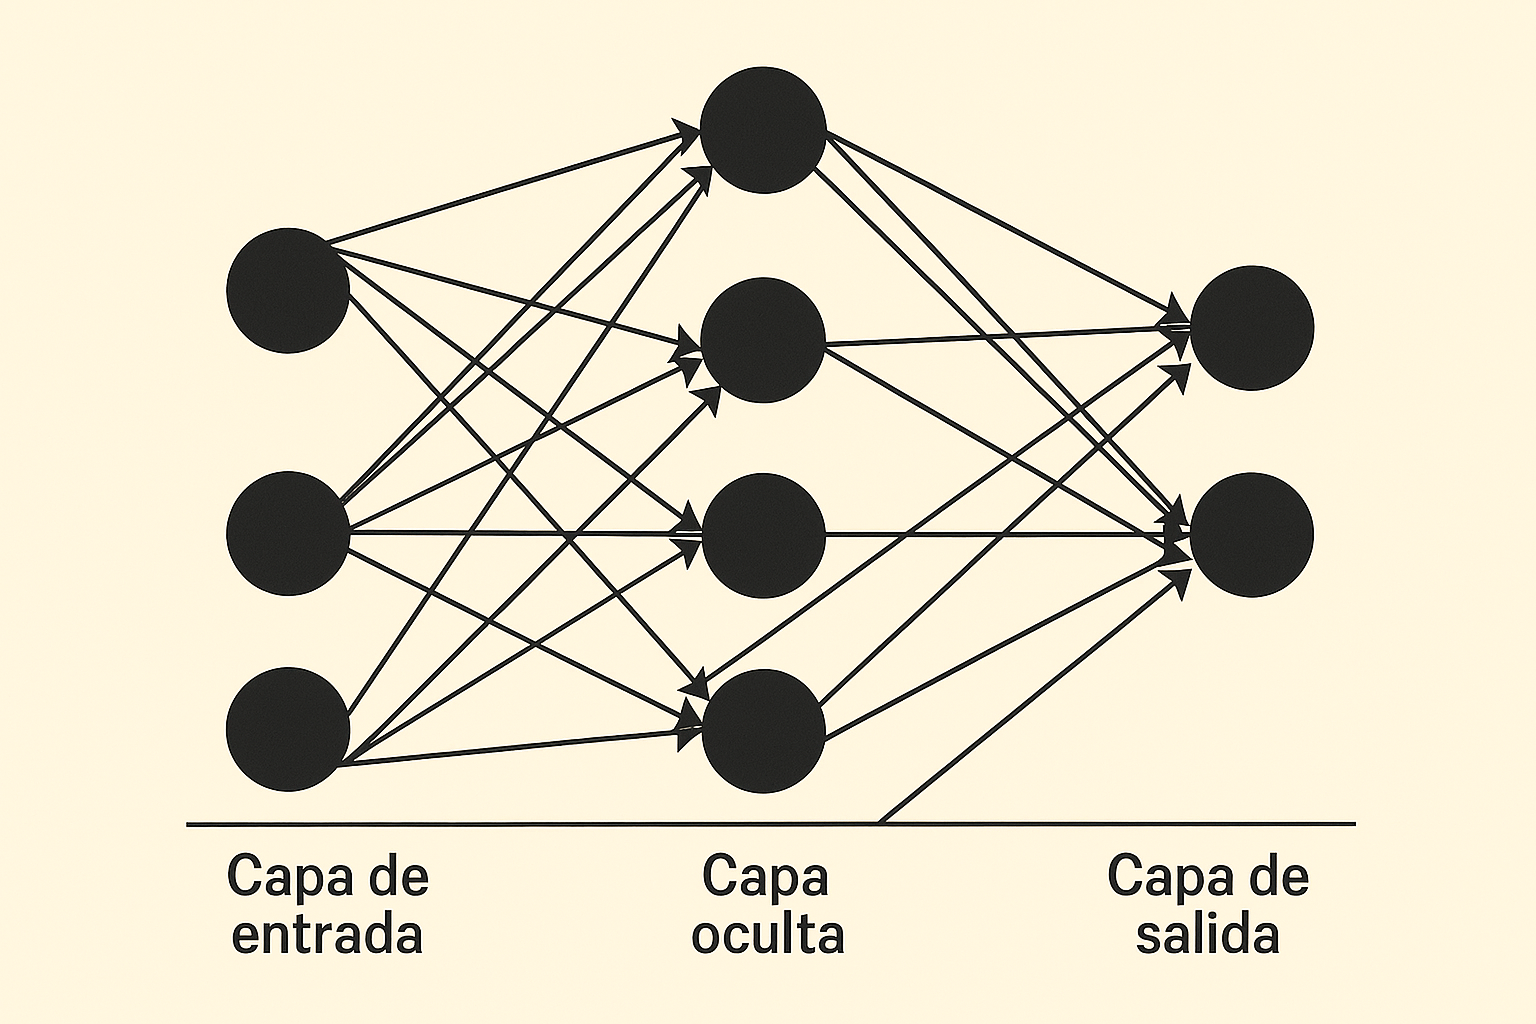
\includegraphics[scale=0.25]{imgss215.png}
	\caption{Diagrama de modelo de red neuronal artificial. Imagen generada con recursos de Internet}
	\label{fig:figura700_6}
\end{figure}

El ejemplo mostrado en la \autoref{fig:figura700_6} es un ejemplo básico en cuanto a tamaño de la red, pero suficiente para explicar en qué consiste y cómo se ampliaría a una arquitectura más general.

Cada uno de los puntos de color negro corresponde a una neurona o nodo, y cada uno de ellos mantiene una conexión con otras neuronas, tanto previas como posteriores. Toda Red Neuronal está compuesta por \textbf{\textit{capas}},
que son cada una de las columnas de nodos, en nuestro caso tenemos 3 capas. Dentro de esta característica, igualmente en cualquier Red Neuronal encontraremos 3 tipos de capas: la \textbf{\textit{capa de entrada o input layer}},
\textbf{\textit{capas ocultas o hidden layers}} y \textbf{\textit{capa de salida o output layer}} \cite{deitelIA}. 

La capa de entrada es siempre la columna de nodos que se encuentra más a la izquierda en el diagrama; en ella se colocan tantos nodos como número de variables de entrada con las que se va a trabajar. La capa de salida es siempre la columna de neuronas que se encuentra más a la derecha del diagrama; el número de nodos a colocar en esta capa es igual al número de variables de salida que se requieren. 

Por ejemplo, si la Red Neuronal va a trabajar como un algoritmo de regresión, únicamente se colocará un nodo en la capa de salida, el cual corresponderá a la variable target que se 
busca predecir. Si la Red Neuronal se planteará para usarse como algoritmo de clasificación, el número de nodos en la capa de salida sería igual al número de clases posibles en el problema de clasificación que se busca resolver.

Finalmente, las capas ocultas son todas las columnas de nodos que se encuentren entre la capa de entrada y la capa de salida; en nuestro ejemplo solo se muestra 1 capa oculta, pero se pueden colocar las que sean necesarias 
de acuerdo a las necesidades del problema a resolver. Referente al número de nodos en cada capa oculta, igualmente se pueden colocar la cantidad que sea necesaria acorde al propósito que tenga la Red Neuronal \cite{AurelienGeron}. 

Es necesario aclarar que mientras mayor sea el número de capas ocultas y nodos en cada una de ella, el modelo matemático generado será mucho más complejo y más difícil de procesar a nivel de cálculo computacional, pero es 
precisamente el generar una Red de mayor tamaño lo que permite resolver problemas más complejos, es decir, una Red Neuronal con 1 capa oculta y 20 nodos en ella tendrá menor capacidad de aprendizaje
para resolver un problema de alta complejidad que una Red con 10 capas ocultas y 50 nodos en cada una de ellas.

En la \autoref{fig:figura700_6}, también se muestran las conexiones existentes entre las neuronas de diferentes capas, teniendo en este caso que cada neurona de la capa de entrada se conecta a todas las neuronas de la capa 
oculta; las neuronas de la capa oculta se conectan a todas las neuronas de la capa previa y la capa posterior, ya sea que la capa posterior sea otra capa oculta o la capa de salida y la capa previa sea la capa de entrada u 
otra capa oculta. 

La conexión entre 2 neuronas cualesquiera está definida siempre por un peso sináptico, los cuales servirán como coeficientes para una combinación lineal de todas las entradas a una neurona específica, y dicha combinación 
lineal será la entrada para la función de activación de cada neurona. Es decir, por ejemplo para la \autoref{fig:figura700_6}, a cada una de las neuronas de la capa oculta su entrada es la combinación lineal de las señales
provenientes de la capa de entrada, y las neuronas de la capa oculta evaluan esa combinación mediante su función de activación, la cual emite una señal de salida. Por lo tanto, de la capa oculta se tendrán 4 señales de 
salida, cada una proveniente de nodos distintos, y estas señales ahora serán las que servirán para formar combinaciones lineales que serán las entradas a las neuronas de la capa de salida, las cuales nuevamente evalúan las
combinaciones mediante sus funciones de activación para poder entregar señales de salida, las cuales en este caso ya serían el resultado final.

Por último, tanto en las capas ocultas como en la capa de salida, otro elemento importante es el término individual de \textit{bias} o \textit{sesgo} que corresponde a cada una de estas capas en la red; estos términos son 
valores numéricos constantes de inicio y que pueden modificar sus valores también cuando se realiza la optimización de los pesos sinápticos durante el entrenamiento de la red. De forma matemática, cada uno de estos términos 
se convierte en otro elemento o término adicional para cada una de las combinaciones lineales formadas para cada nodo de las capas ocultas y capa de salida.

La principal función de los terminos bias es evitar que los nodos de una red neuronal emitan una señal de salida de 0 cuando los valores de entrada son 0 para ese conjunto específico de nodos en el modelo. Esto evita que 
se anulen o hagan 0 los valores propagados hacia adelante a través de la red, además de que estos términos bias ayudan a generar patrones matemáticos o geométricos más complejos, lo que hace al modelo tener mejores resultados.

\subsection{Funciones De Activación}

En una Red Neuronal es posible tener 1 sola función de activación en todas las capas, o por ejemplo una función específica para las capas ocultas y otra función diferente para los nodos de la capa de salida. Todo dependerá 
del tipo de aplicación que va a desarrollar el modelo. A continuación se describen las funciones más comunes.

\textbf{\textit{Función ReLU (Rectified Linear Unit, Unidad Rectificada Lineal)}}. Se define de la forma (\ref{eq:ecuacion724}).

\begin{equation}
	f(x)=\textbf{max} (0,x)
	\label{eq:ecuacion724}
\end{equation}

Su gráfica se muestra en la \autoref{fig:figura700_7}.

\begin{figure}[h]
	\centering
	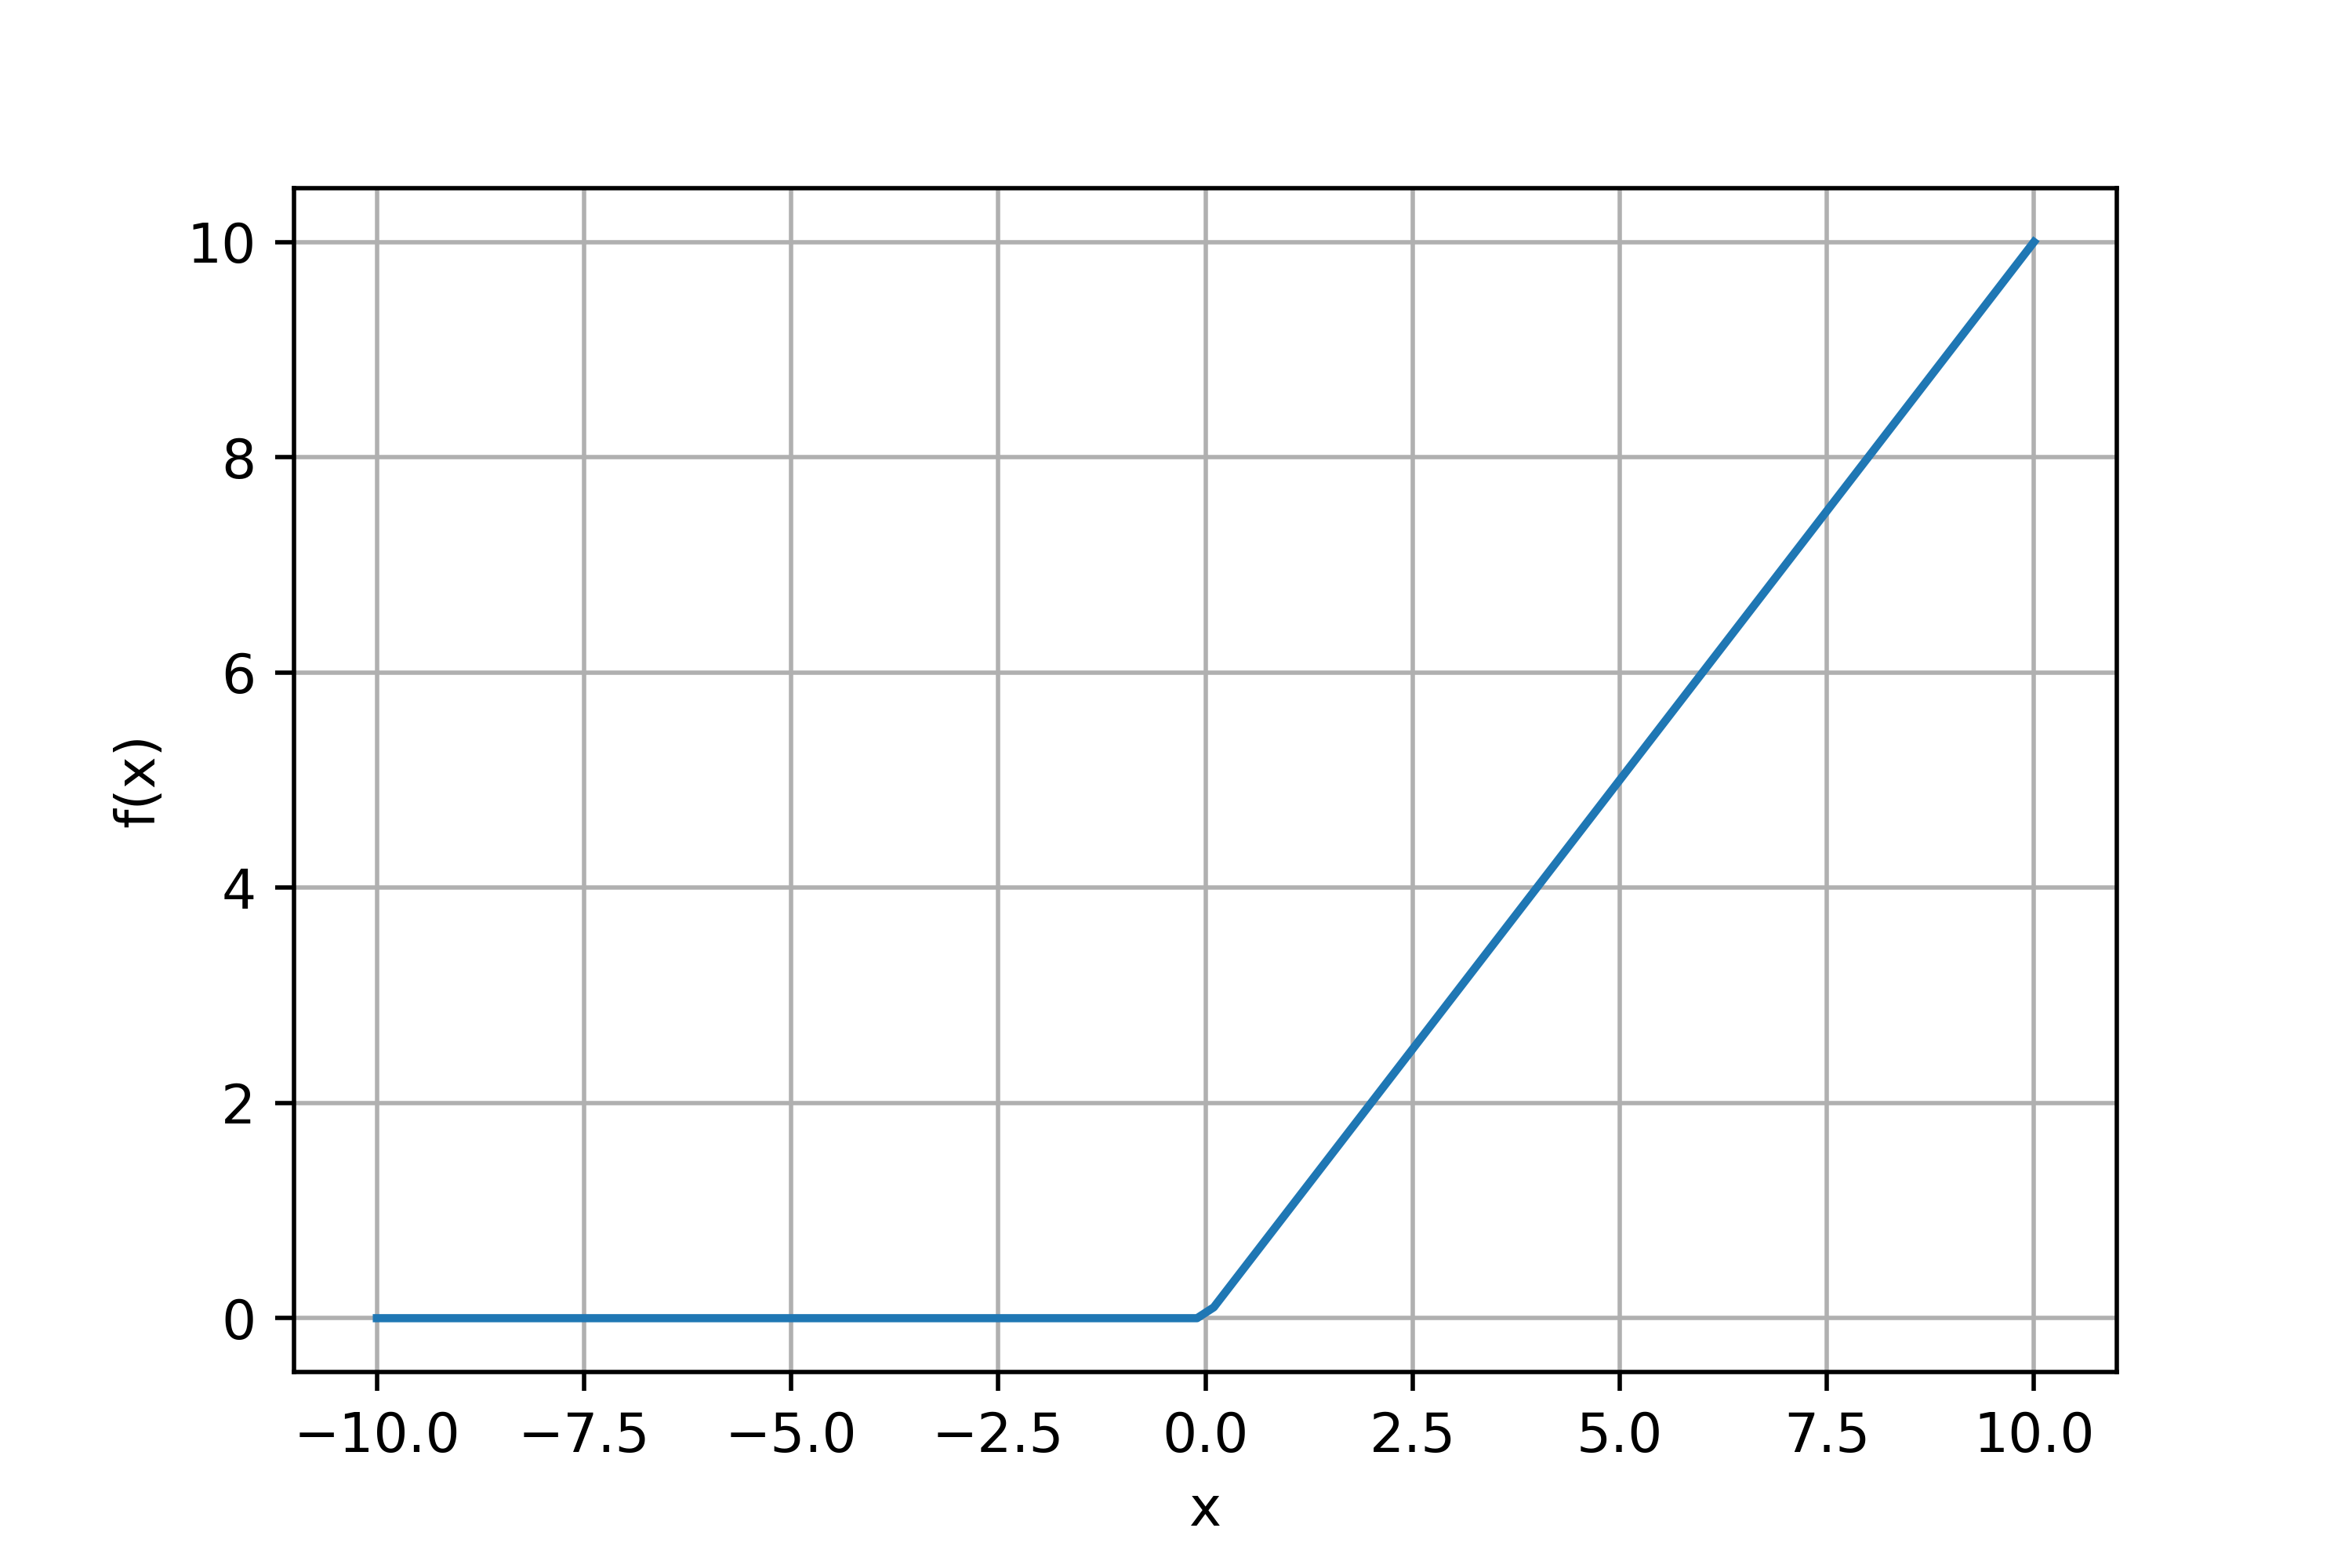
\includegraphics[scale=0.8]{imgss149.png}
	\caption{Función ReLU}
	\label{fig:figura700_7}
\end{figure}

Se trata de una función de tipo rampa, la cual al ser negativa la variable de entrada, la salida entregada es 0; si la entrada a la función es positiva, entonces el valor a la salida es igual al valor a la entrada. Dado 
lo anterior, en una red neuronal esta función permite eliminar cualquier valor negativo generado por las ecuaciones implícitas en el algoritmo \cite{ReluBarcelona}.

Entre las ventajas que ofrece están la de acelerar la convergencia del algoritmo de optimización de descenso por gradiente para casos específicos en comparación con otras funciones de activación diferentes, además de que 
su implementación en código resulta muy simple. Una desventaja importante que posee tiene que ver con el hecho de que es una función que puede llegar a \textit{morir}, es decir, que durante el proceso de optimización de 
los pesos de la red, se llegue a una circunstancia donde dicha función nunca vuelva a dispararse, siendo 0 su salida sin posibilidad de revertir este efecto \cite{ReluBarcelona}.

\textbf{\textit{Función sigmoide}}. Se define de la forma (\ref{eq:ecuacion725}).

\begin{equation}
	\sigma(x)=\frac{1}{1+exp(-x)}
	\label{eq:ecuacion725}
\end{equation}

Su gráfica se muestra en la \autoref{fig:figura700_8}.

\begin{figure}[h]
	\centering
	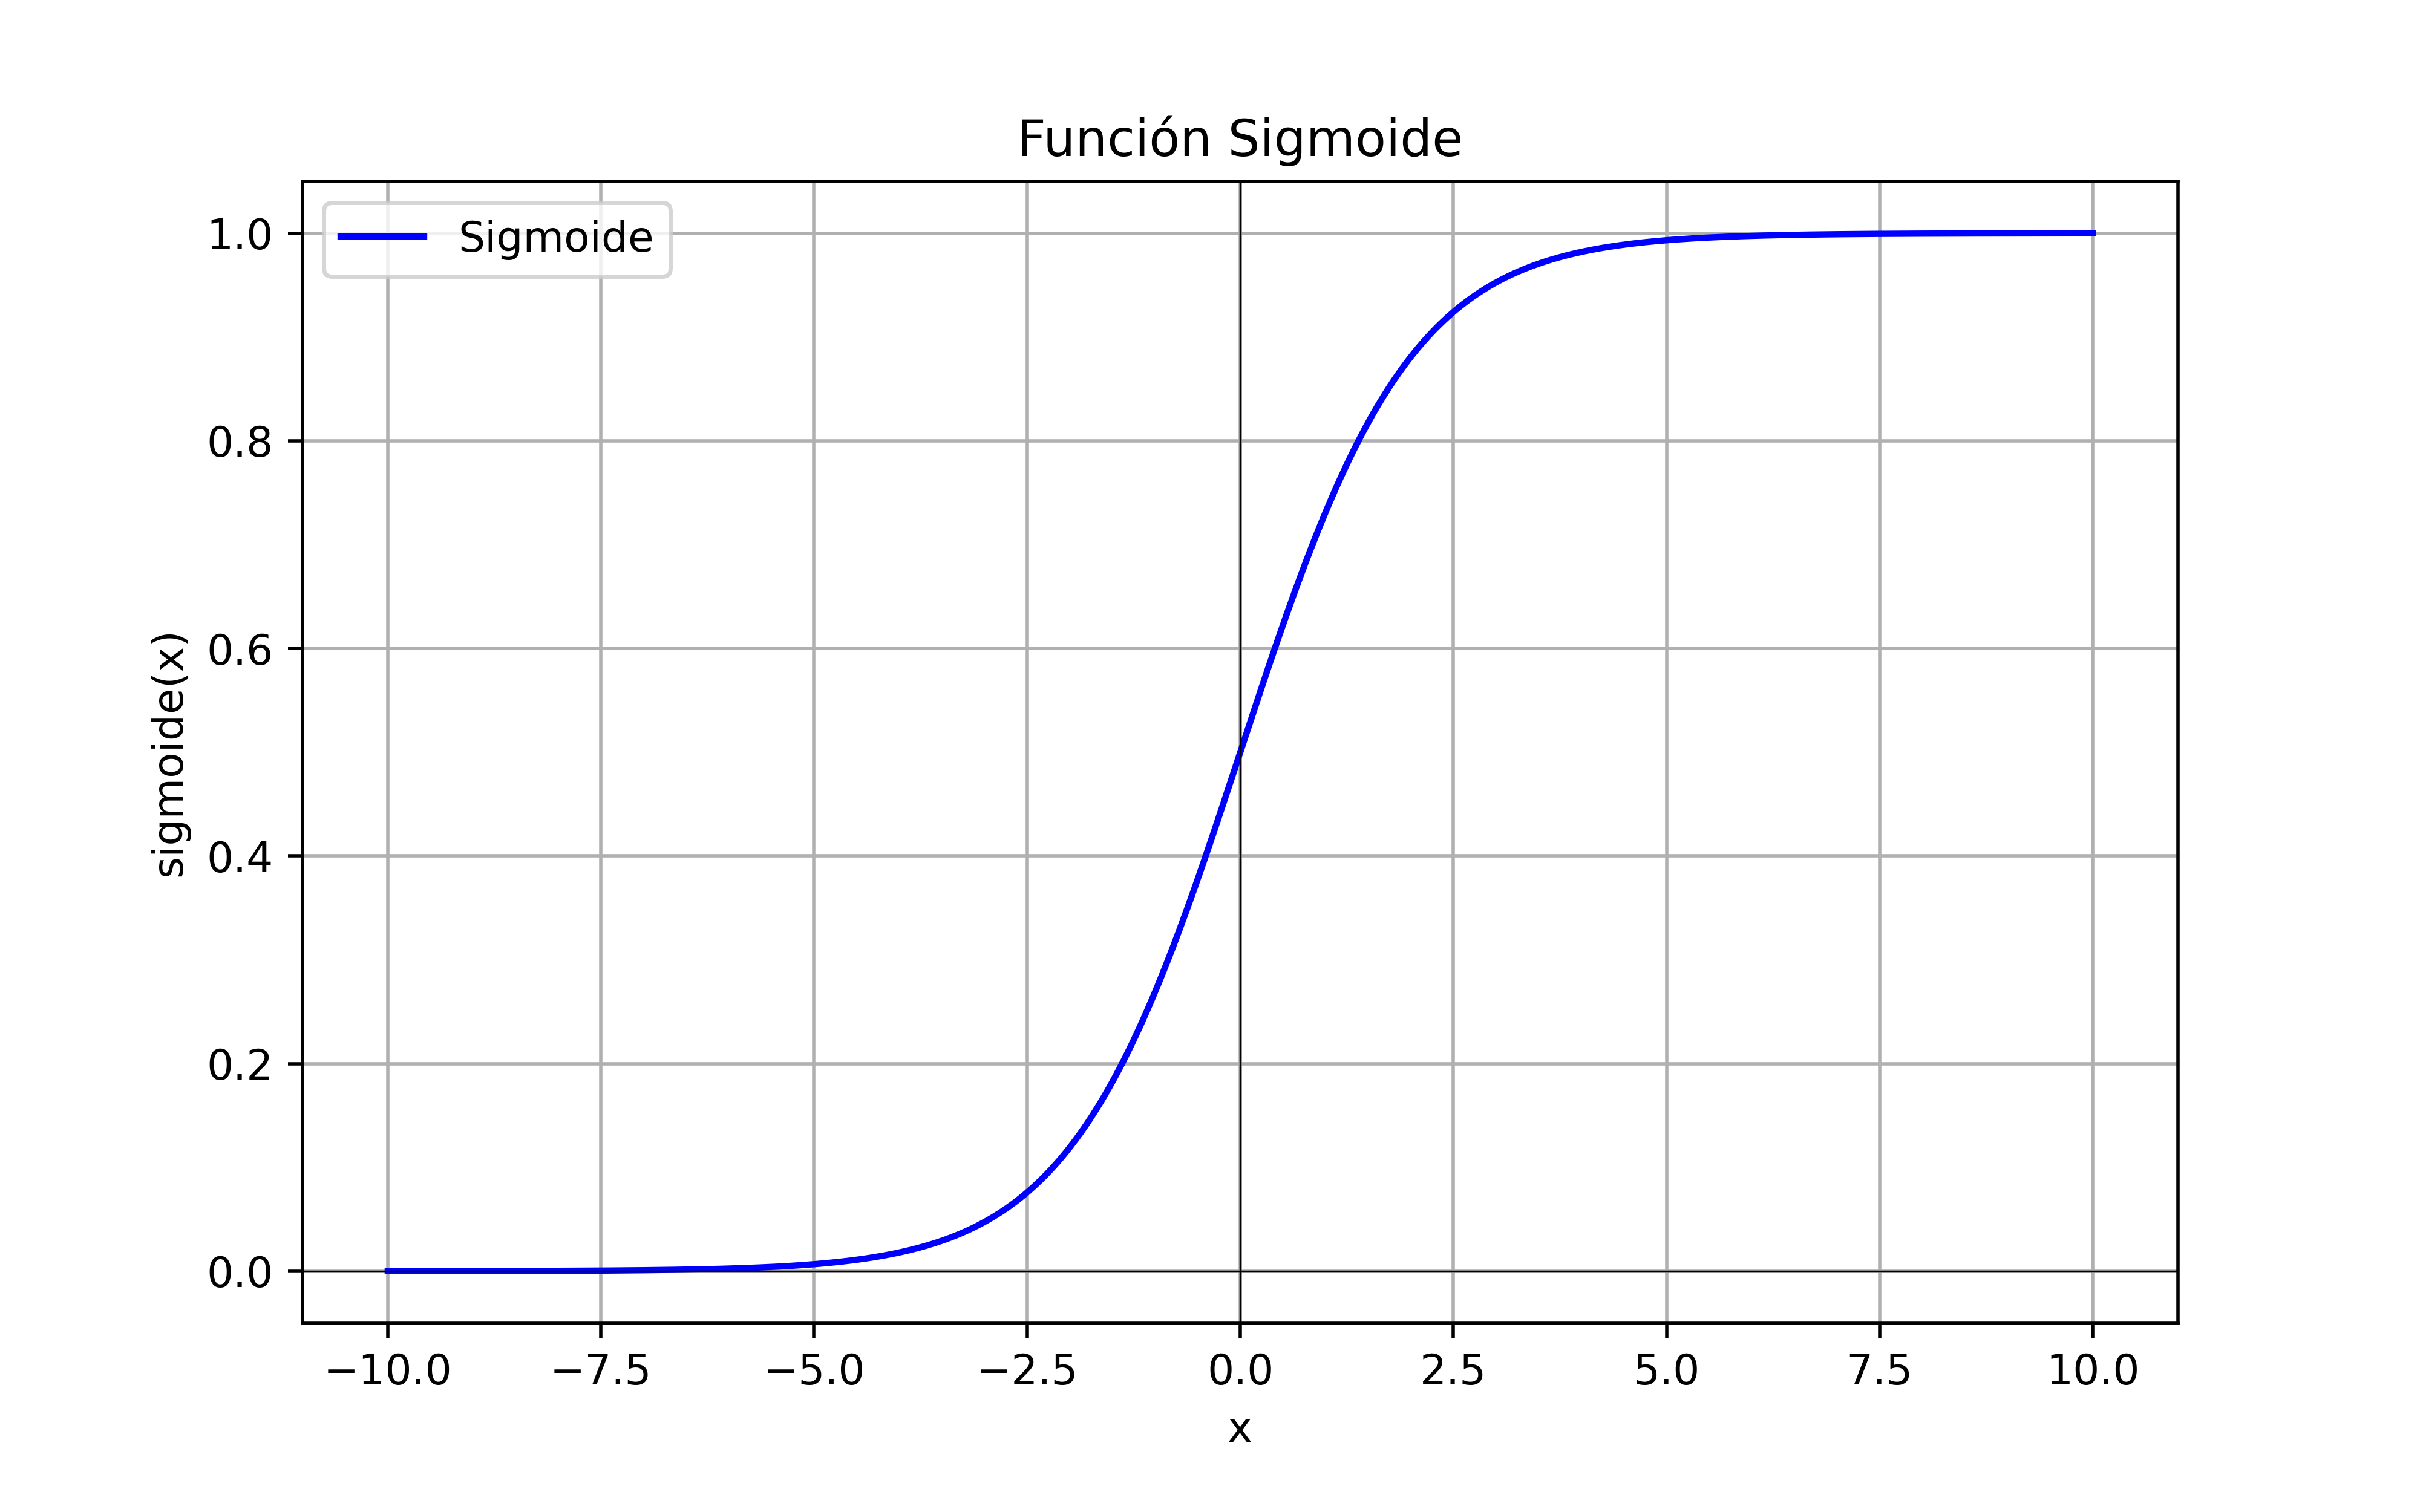
\includegraphics[scale=0.8]{imgss205.png}
	\caption{Función Sigmoide}
	\label{fig:figura700_8}
\end{figure}

Es una función de tipo exponencial que para valores cercanos a 0 en la variable de entrada, cambia de forma acelerada su valor de salida de un valor muy cercano a 0 a un valor muy cercano a 1 y viseversa. 
Indicando también que para un valor de entrada de \textit{x=0}, la función toma 0.5 como valor.
Para valores negativos a la entrada, la función tiene un comportamiento asintótico sobre el valor de 0, y para valores positivos de entrada la función tiene también un comportamiento asintótico, pero ahora sobre el valor de 1 \cite{SeriesTemporalesAvanzadas}.

Entre sus propiedades, permite que en la Red Neuronal se tengan valores de salida de cada una de las capas en un rango de 0 a 1, logrando así no tener valores que se disparen a magnitudes elevadas, sobre todo cuando los 
rangos de valores de las variables de entrada a la Red son muy distintos. Una razón por la cual también es importante hacer un escalamiento de los valores de entrada a la Red cuando se usa esta función \cite{RNAlineasDeTransmisión}. 

Adicionalmente, facilita las aplicaciones destinadas a problemas de clasificación binaria, es decir, únicamente 2 clases posibles. Esto se logra debido a que se aprovecha la propiedad de la función de que conmuta entre 0 
y 1 \cite{RNAlineasDeTransmisión}. 

\textbf{\textit{Tanh (Función Tangente Hiperbólica)}}. Se define de la forma (\ref{eq:ecuacion726}):

\begin{equation}
	tanh(x)=\frac{exp(x) - exp(-x)}{exp(x) + exp(-x)}
	\label{eq:ecuacion726}
\end{equation}

Su gráfica se muestra en la \autoref{fig:figura700_9}.

\begin{figure}[h]
	\centering
	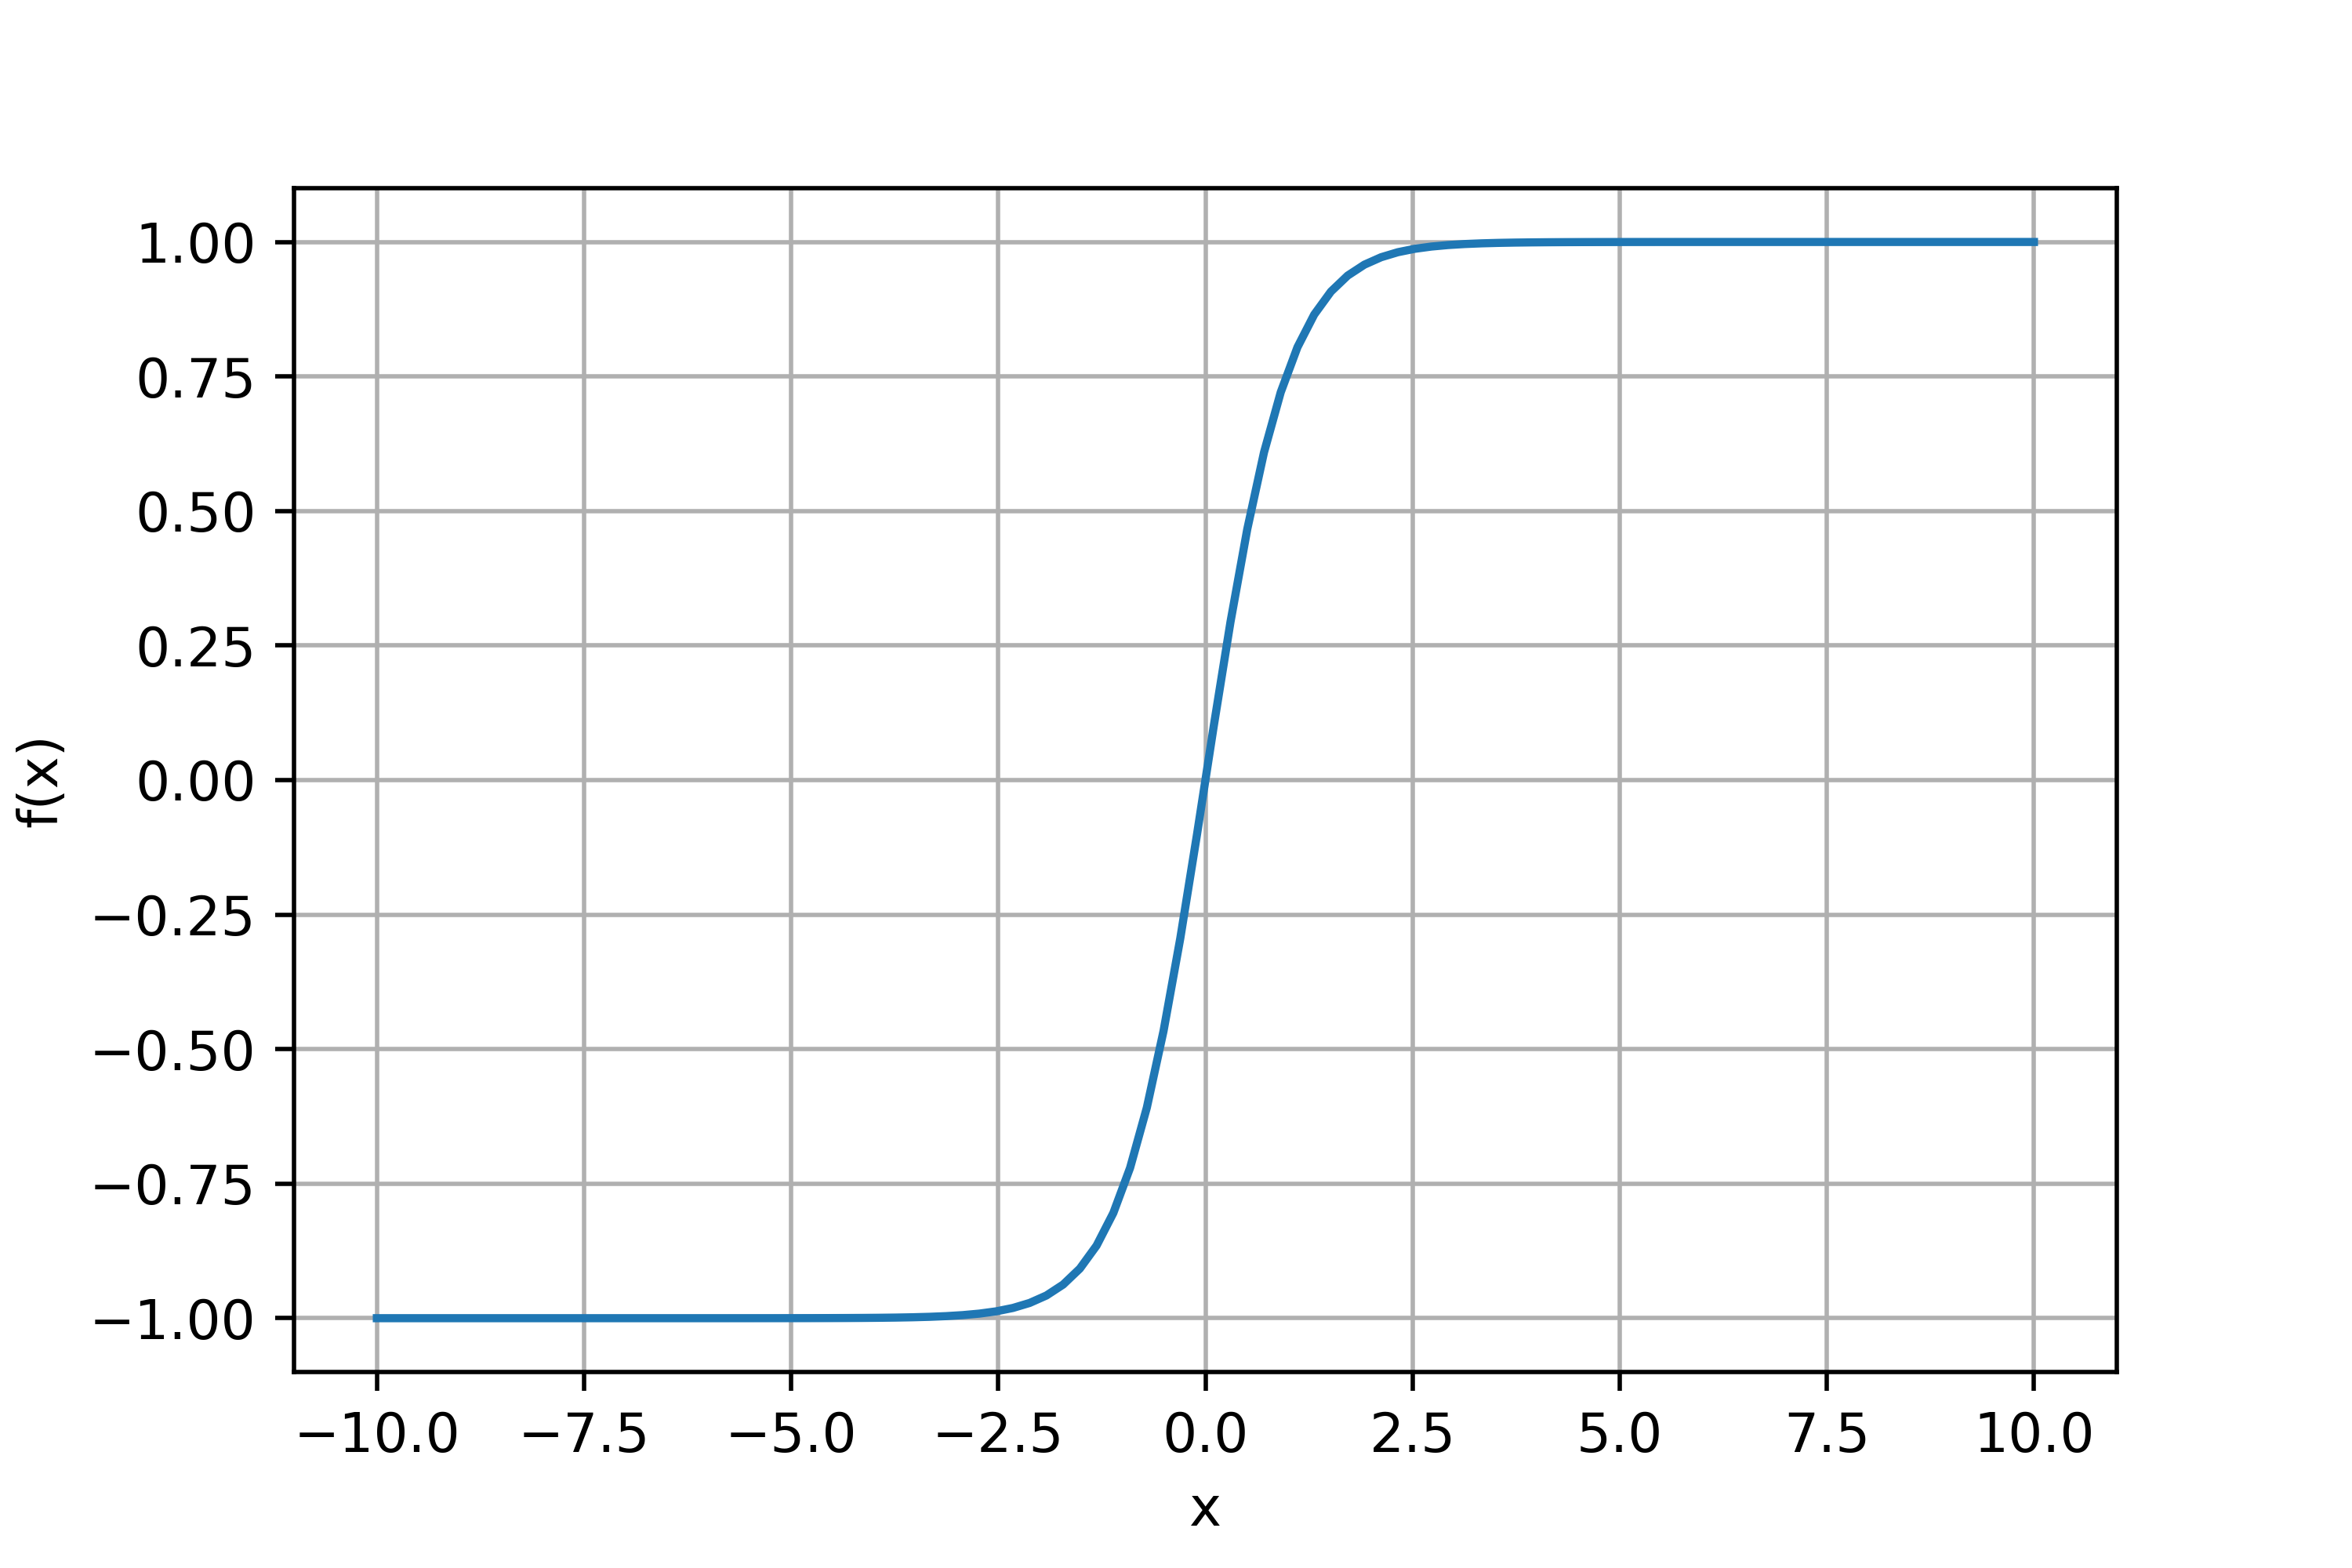
\includegraphics[scale=0.8]{imgss150.png}
	\caption{Función tangente hiperbólica}
	\label{fig:figura700_9}
\end{figure}

En la \autoref{fig:figura700_9} se observa que tiene la misma forma que la función sigmoide, sin embargo, para valores negativos de la variable de entrada ahora el comportamiento asintótico es sobre el valor de -1, y la 
función sigmoide lo hace sobre el valor de 0. Esta diferencia es precisamente un factor importante para elegirla en vez de a la sigmoide, debido a que su rango de valores de salida no se corta en 0, sino que permite también 
entregar valores negativos como señal de salida. 

Otras ventajas que tiene sobre la sigmoide es que suele acelerar la convergencia en la optimización de los pesos sinápticos durante el ajuste del modelo, además de que disminuye 
el efecto de desvanecimiento del gradiente, es decir, que durante el ajuste de la red se generen valores que tiendan a 0, lo cual provoca generalmente que el entrenamiento se vuelva muy lento, es decir, que llegue a 
requerir un número muy grande de iteraciones. En el caso de la aceleración en la convergencia en el entrenamiento de una red neuronal al usar la función tangente hiperbólica, este efecto se debe principalmente a que la sigmoide 
solo tiene salidas con valores positivos, mientras que la función tangente hiperbólica admite salidas con valor negativo lo que permite tener más estabilidad en la magnitud de los \textit{saltos} dados en el proceso de descenso 
por gradiente \cite{RNAconceptosBasicos}.

\textbf{\textit{Función Softmax}}. Se define de la forma (\ref{eq:ecuacion727}).

\begin{equation}
	f(x)_j=\frac{exp(x_j)}{\sum_{i=1}^{K} {exp(x_i)}}
	\label{eq:ecuacion727}
\end{equation}

El factor \textit{K} es el número de clases posibles en el clasificador; el subíndice \textit{j} hace referencia a la j-ésima clase.

La función softmax usualmente es aplicable en problemas de clasificación, ya que permite calcular la probabilidad de cada clase sobre todas las clases posibles, factor que la convierte en una opción efectiva para casos de 
clasificación multiclase. Una función con esta forma se puede aprovechar para colocarse en los nodos de la capa de salida de una Red Neuronal, debido a que entregará como resultado un rango de probabilidad de salida entre 
0 y 1, teniendo que la suma de todas las probabilidades dará un resultado de 1 \cite{tanhArgentina}.

\textbf{\textit{Función Lineal}}. Se define de la forma (\ref{eq:ecuacion728}).

\begin{equation}
	f(x)=x
	\label{eq:ecuacion728}
\end{equation}

Lo que nos dice la ecuación (\ref{eq:ecuacion728}) es que la salida entregada por esta función es igual a la señal que recibe a la entrada.

El caso más significativo de uso de esta función es en la capa de salida en problemas de regresión. Esto es debido a que en este tipo de problemas se busca predecir una valor numérico target único, por lo tanto al usar esta 
función se asegura que el modelo entregará un resultado numérico al que no se le halla aplicado ninguna transformación matemática \cite{RNAconceptosBasicos}.

En el caso contrario, en las capas ocultas de una Red Neuronal no es recomendable el uso de la función lineal debido a que lo que se busca en las capas ocultas es generar patrones no lineales complejos, que son precisamente 
los que permiten abordar con éxito la mayoría de las aplicaciones \cite{RNAconceptosBasicos}.

\subsection{Entrenamiento De Una Red Neuronal}

Sea cual sea el propósito que se le dé a una Red Neuronal, ya se ha mencionado que el modelo debe optimizarse o entrenarse para poder llegar a la mejor aproximación posible en el conjunto de pesos sinápticos que forman parte 
del modelo. Dicho entrenamiento requiere \textbf{\textit{datos}}, pero de dónde deben surgir o conseguirse; todo depende del problema que se quiera resolver. Si el modelo se usará para procesamiento de audio, entonces los 
datos deben recolectarse de señales de audio; si se busca hacer procesamiento de imagen, consecuentemente los datos deben provenir de imágenes.

La idea es que para el propósito que tenga la Red Neuronal, se requiere obtener la mayor cantidad de información posible acerca del fenómeno, proceso o procedimiento en donde se busca trabajar con el algoritmo; se necesita 
establecer un conjunto de variables o parámetros característicos de los cuales obtener la mayor cantidad de valores posibles de cada uno de ellos, y dicha información formará el conjunto de datos que nos permitirá aplicar 
una metodología conocida como \textbf{\textit{Feed-Forward o Propagación Hacia Adelante}}. 

Una vez que se ha recolectado toda la información para el conjunto de datos o \textit{dataset} para el modelo, es necesario dividirlo en 2 subconjuntos; el primero, para el entrenamiento del modelo, y el segundo para realizar 
la \textit{validación} del modelo, es decir, verificar qué tan bien el modelo es capaz de entregar los resultados requeridos. Dicha fragmentación del dataset generalmente suele realizarse asignando el 80$\%$ de todos los 
datos para entrenamiento y el 20$\%$ restante para validación; otra convención también usada ampliamente es asignar el 70$\%$ de los datos para entrenamiento y el 30$\%$ restante para validación \cite{caicedoANN}.

Aparte del método Feed-Forward ya mencionado, el segundo procedimiento a ejecutar para lograr el ajuste de la Red Neuronal es el método de \textbf{\textit{Error Backpropagation, Propagación Hacia Atrás del Error}}. La aplicación
de estos 2 métodos nos permitirá obtener información sobre el estado de la Red Neuronal durante el entrenamiento, lo cual finalmente nos permitirá aplicar el algoritmo de descenso por gradiente para minimización de la función 
de costo.

La aplicación del método Feed-Forward consiste en propagar los datos de entrenamiento de izquierda a derecha a través de la Red Neuronal, es decir, primeramente se tiene la capa de entrada que no aplica función de activación 
alguna. Posteriormente los datos deben propagarse de forma distribuida a través de todos los nodos de todas las capas ocultas. Finalmente,
las señales de salida de la última capa oculta son entrada para la capa de salida, la cual se encarga de entregar el resultado final.

Lo descrito en el párrafo anterior se debe realizar de forma iterativa con todos los datos de entrenamiento disponibles, pero entre cada iteración individual es necesario realizar un ajuste de todos los pesos del modelo tomando 
como referencia el error puntual que se tiene en la salida de la red para cada target. Es en esta parte donde se requiere trabajar con una función de costo o error, la cual sea una función 
matemática que tenga como variables independientes al conjunto de pesos del modelo, y con la cual se pueda trabajar el algoritmo de descenso por gradiente para buscar un valor mínimo global del error y al mismo tiempo encontrar 
la mejor optimización de los pesos sinápticos \cite{BobadillaML}. 

Dado que el error dado en la capa de salida se utiliza como referencia para determinar el nivel de optimización de los pesos en las capas anteriores, es por esta razón que se 
denomina como Propagación Hacia Atrás del Error, ya que el error dado en la salida de la Red Neuronal se distribuye hacia atrás hacia todas las conexiones sinápticas del modelo, y de esta forma poder determinar la 
cantidad de cambio que se aplicará a cada peso en cada iteración durante el proceso de entrenamiento \cite{BobadillaML}.

Una red neuronal consiste en generar funciones no lineales de combinaciones lineales de las entradas. Primeramente, para la capa de entrada si se tiene un conjunto \textit{$x_1$, $x_2$, ... , $x_D$} como variables para el 
modelo, entonces se pueden definir \textit{M} combinaciones lineales de las entradas de la forma (\ref{eq:ecuacion729}).

\begin{equation}
	a_j=\sum_{i=1}^{D} {w_{ji} x_i + w_{j0}}
	\label{eq:ecuacion729}
\end{equation}

donde \textit{j=1,2,...,M} se refieren al número de nodos existentes en la capa siguiente. En la ecuación (\ref{eq:ecuacion729}) también es importante señalar al segundo término en el lado derecho de la ecuación, el cual viene siendo 
el término \textit{bias} para cada uno de los nodos de la capa oculta. El subíndice \textit{i} hace referencia al i-ésimo dato de entrada a la red neuronal; el elemento \textit{$a_j$} es la combinación lineal de entrada 
al j-ésimo nodo de la capa siguiente y \textit{D} es el número total de datos de entrada a la red \cite{bishop}. 

En la \autoref{fig:figura700_200} se muestra un diagrama que ejemplifica lo anteriormente descrito.

\clearpage

\begin{figure}[h]
\centering
  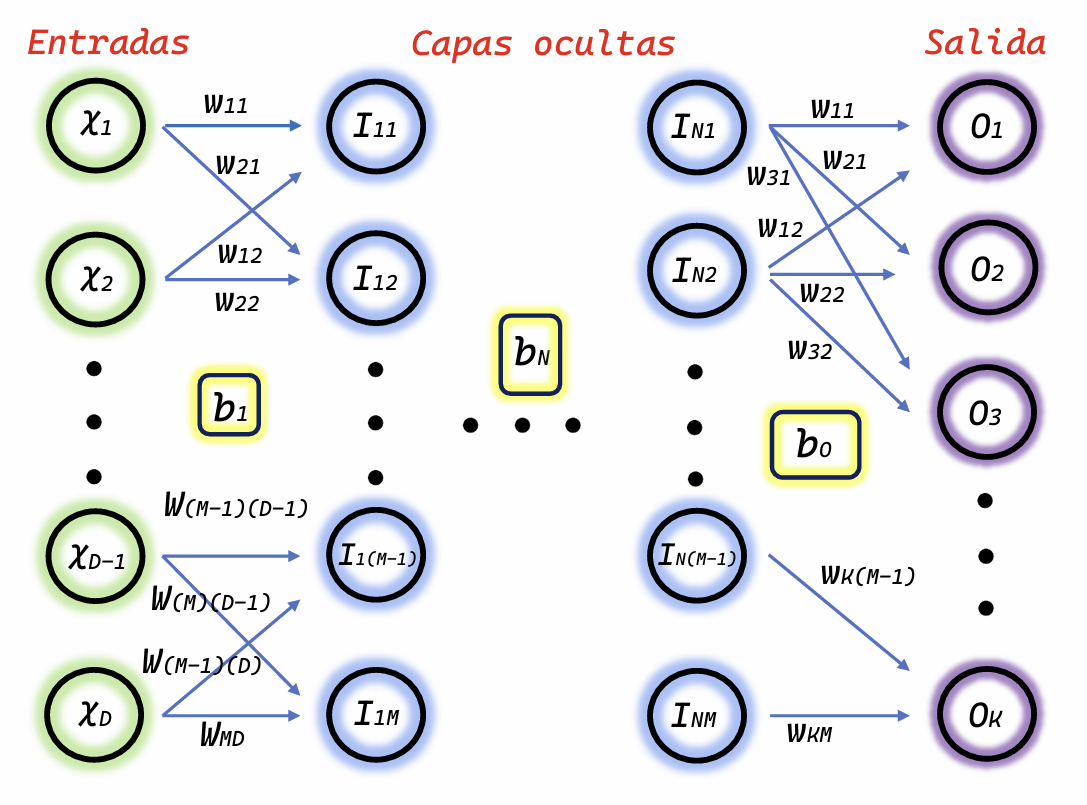
\includegraphics[scale=0.8]{imgss222.png}
  \caption{Representación general de red neuronal}
  \label{fig:figura700_200}
\end{figure}

La \autoref{fig:figura700_200} muestra una representación general con una capa de entrada compuesta por \textit{D} elementos, un número \textit{N} de capas ocultas, cada una de ellas con \textit{M} nodos; en la capa de salida 
se muestra un número \textit{K} de nodos. Adicionalmente, se muestran los términos \textit{$b_1$}, \textit{$b_N$} y \textit{$b_O$}, que son los términos bias correspondientes a capas ocultas y capa de salida, respectivamente. 

Ahora, cada uno de los términos \textit{$a_j$} son transformados usando una función de activación \textit{h} de la forma (\ref{eq:ecuacion730}).

\begin{equation}
	z_j=h(a_j)
	\label{eq:ecuacion730}
\end{equation}

Como ya se explicó en la Sección 2.4.4, se pueden escoger diferentes funciones de activación dependiendo del tipo de problema que se busca resolver. Ahora, los resultados dados por la ecuación (\ref{eq:ecuacion730}) serán 
las entradas para la siguiente capa de la red, que puede ser la capa de salida u otra capa oculta. Si el modelo solo consta de una capa oculta, se tiene la ecuación (\ref{eq:ecuacion731}), donde se forman las combinaciones 
lineales para la capa de salida, usando los resultados entregados por la capa oculta.

\begin{equation}
	a_k=\sum_{j=1}^{M} {w_{kj} z_j + w_{k0}}
	\label{eq:ecuacion731}
\end{equation}

donde \textit{k=1,2,...,K}, y \textit{K} es el número total de salidas de la red neuronal. De nueva cuenta, el segundo término en el lado derecho en la ecuación (\ref{eq:ecuacion731}) es el término de valores bias, pero en este 
caso los correspondientes a los nodos de la capa de salida. Finalmente, los valores dados por (\ref{eq:ecuacion731}) deben someterse a una última transformación matemática dada por la función de activación que se tenga para 
la capa de salida \cite{bishop}. Por lo tanto, una expresión para la salida de la red puede darse por la ecuación (\ref{eq:ecuacion732}):

\begin{equation}
	y_k(\textbf{x}, \textbf{w})=h( \sum_{j=1}^{M} {w_{kj} z_j + w_{k0}} )
	\label{eq:ecuacion732}
\end{equation}

Es decir, la k-ésima salida \textit{$y_k$}, dependiente de los pesos de enlace y datos de entrada a la red, es igual a la salida de la función de activación dada en la capa de salida, aplicada a la combinación 
lineal de los datos de salida de la última capa oculta y los pesos de enlace entre capa de salida y dicha capa oculta.

El proceso descrito mediante la ecuación (\ref{eq:ecuacion732}) es lo que se ha denominado anteriormente \textit{Propagación Hacia Adelante} de la información a través de toda la red. Este tipo de arquitectura se puede ampliar 
para un número mayor de capas ocultas, lo cual a nivel de ecuaciones implicaría ir agregando una sumatoria adicional por cada capa oculta que se agregue, sin olvidar que cada sumatoria debe llevar su correspondiente vector de términos bias para los nodos de esa capa oculta. Es en este concepto donde se puede apreciar que el agregar más capas 
ocultas nos permite generar expresiones matemáticas más complejas, lo cual consecuentemente nos permitiría resolver problemas de mayor complejidad al tener la posibilidad de formar ecuaciones con la capacidad de replicar 
patrones cada vez más específicos.

Ahora tomemos como referencia la \autoref{fig:figura700_10}. Se hará la suposición de que la superficie de la \autoref{fig:figura700_10} representa para una red neuronal una función de error \textit{E(w)} dependiente de los pesos sinápticos de la red; el objetivo es hallar la mejor optimización 
para los valores de los pesos de forma que se pueda minimizar dicha función de error. Dado que la función \textit{E(w)} es una función \textit{suave} y \textit{continua} dependiente de los pesos, consecuentemente su valor 
más pequeño ocurrirá en un punto tal que su gradiente se \textit{desvanezca}, es decir, sea cero o próximo a dicho valor (\ref{eq:ecuacion733}) \cite{bishop}.

\begin{equation}
	\nabla{E(\textbf{w})} \cong \textbf{0}
	\label{eq:ecuacion733}
\end{equation}

En caso contrario que no tengamos la condición dada por la ecuación (\ref{eq:ecuacion733}), se deben dar \textit{pasos} sobre la superficie en sentido contrario al indicado por el vector gradiente en un punto específico de 
la función con el objetivo de decrementar el error. En una función de error, los puntos donde el gradiente se desvanece se conocen como \textit{puntos estacionarios}, los cuales podrían ser tanto un mínimo o un máximo, o 
incluso un \textit{punto de silla}, que son puntos en la superficie donde el vector gradiente es 0, pero no corresponde a ser ni un mínimo ni un máximo \cite{bishop}.

\begin{figure}[h]
	\centering
	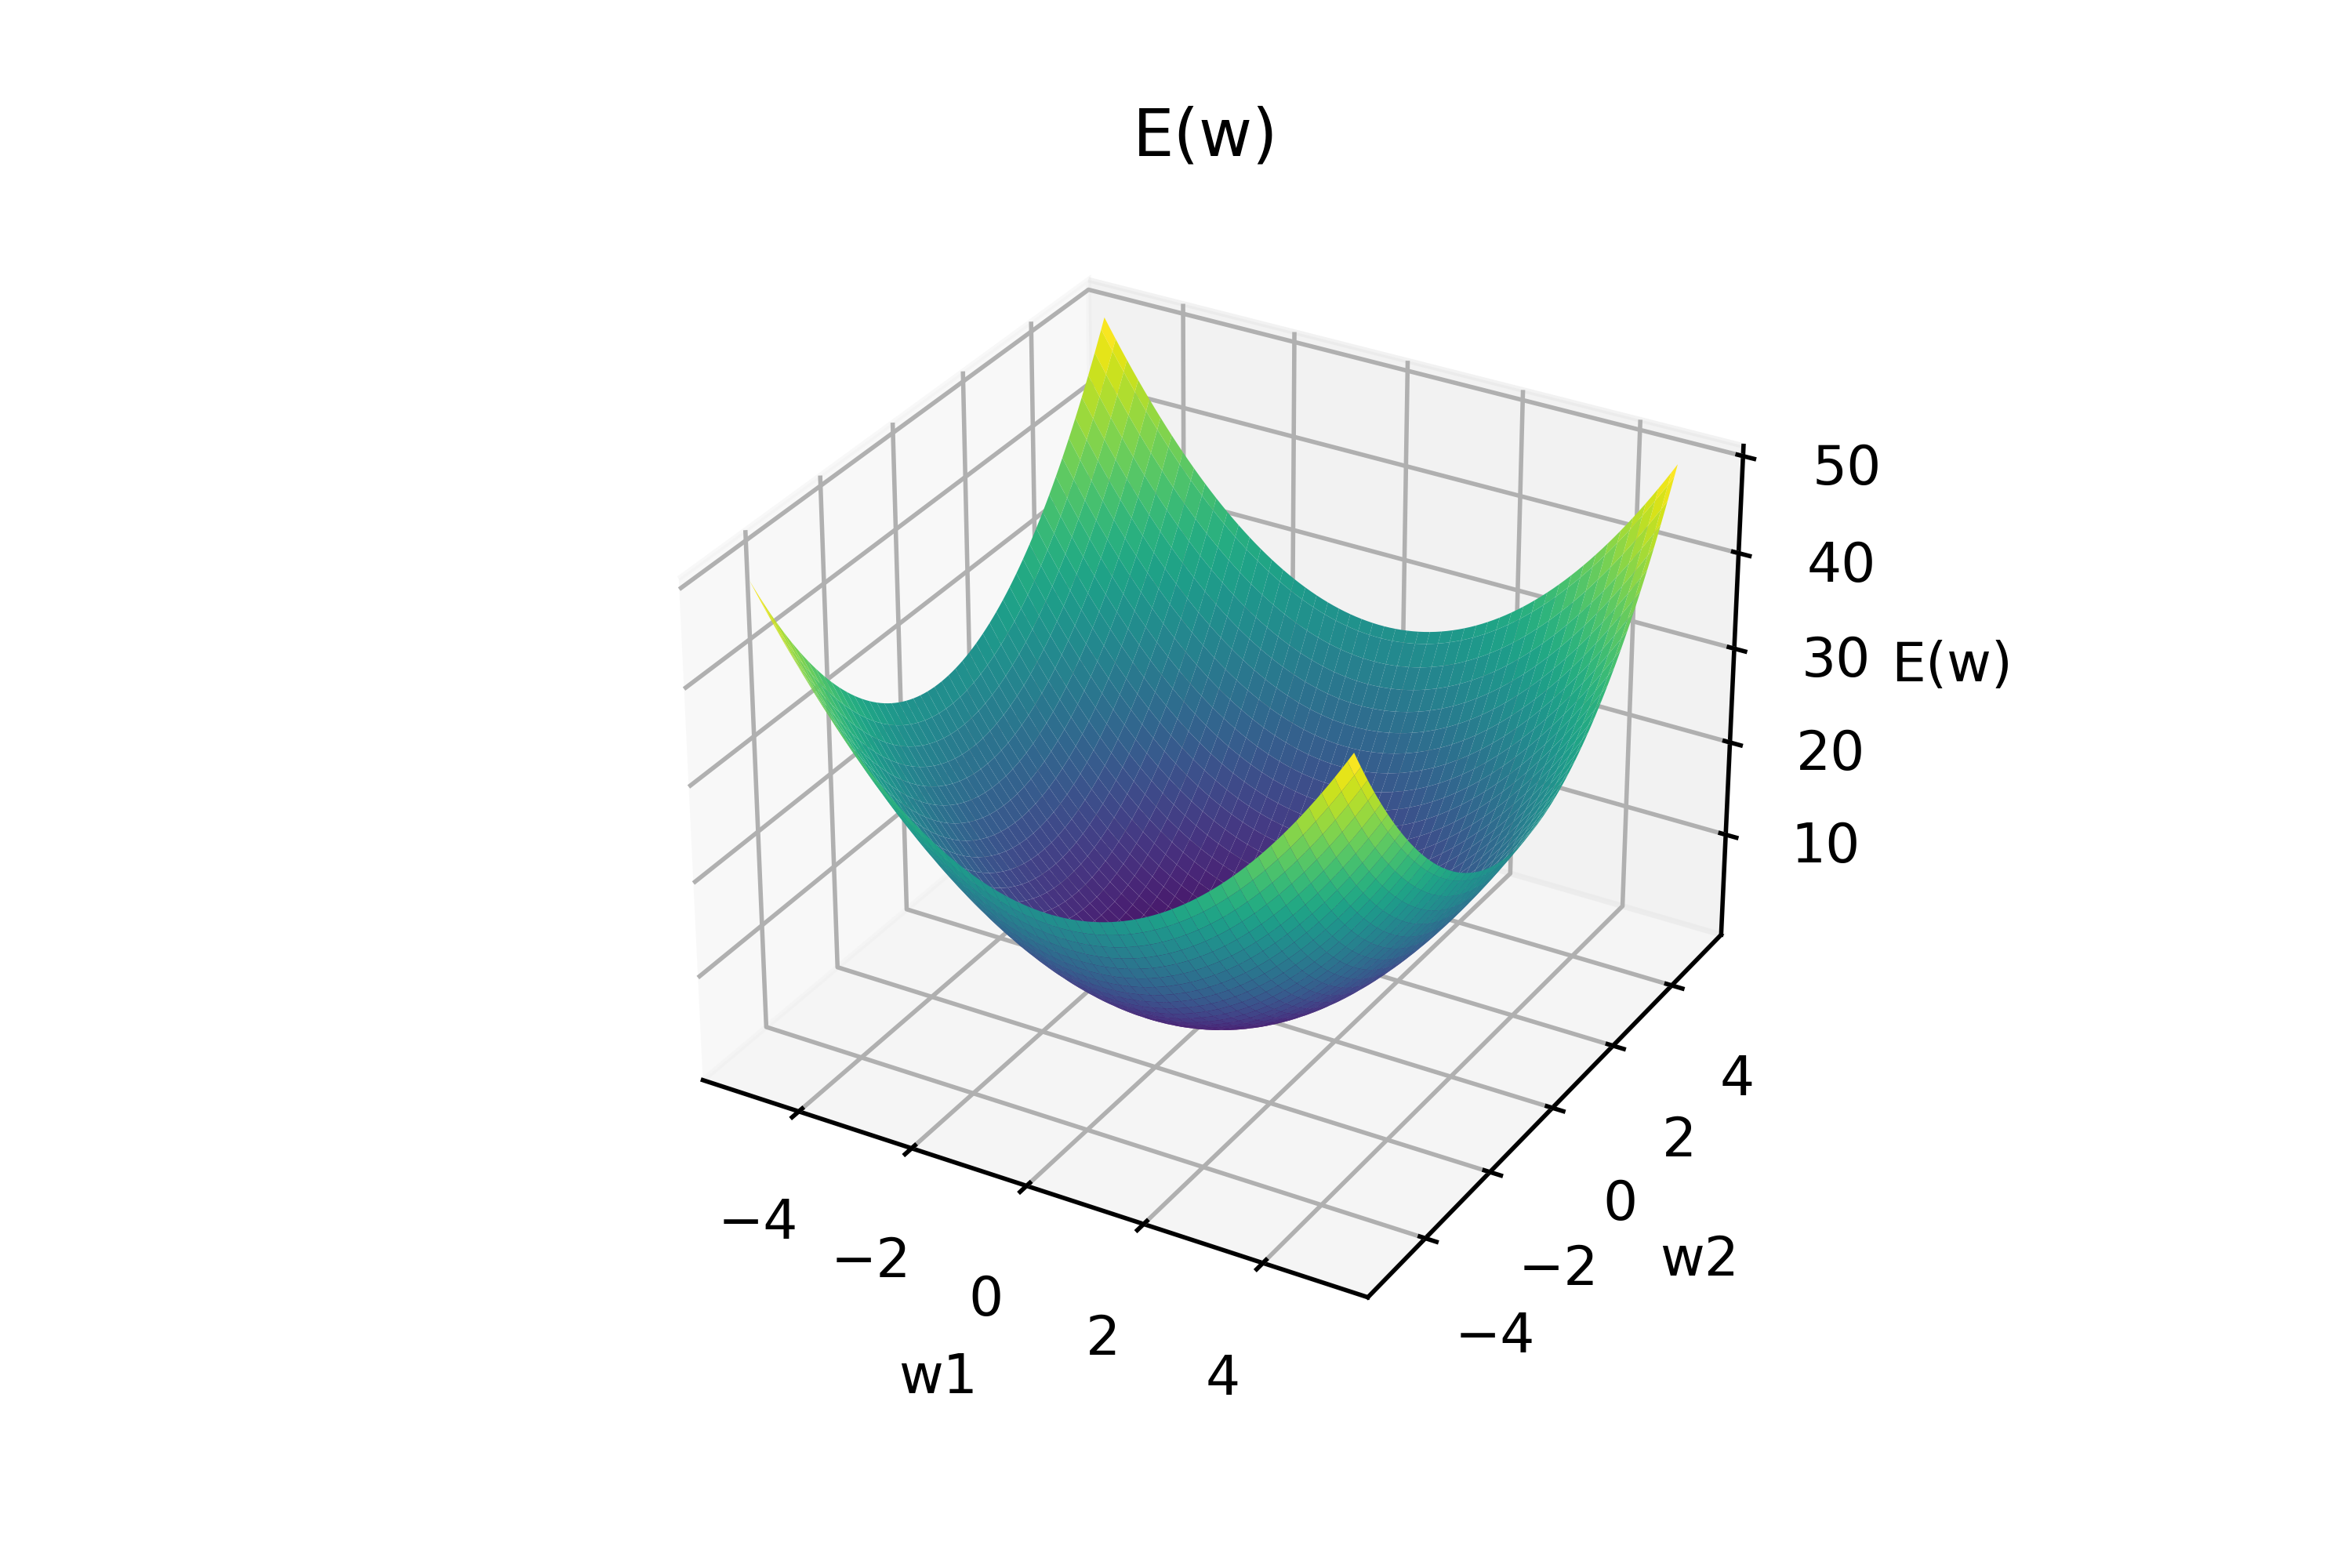
\includegraphics[scale=1]{imgss220.png}
	\caption{Ejemplo de Función de Error E(w)}
	\label{fig:figura700_10}
\end{figure}

Dado que una función de error tendrá una alta dependencia no lineal sobre los pesos y los términos bias de la red, sobre la función se pueden llegar a presentar diversos puntos en los que el gradiente se desvanezca, o numéricamente 
tenga una magnitud muy pequeña. Un punto mínimo que corresponda al valor más pequeño que pueda tomar la función de error dado un conjunto específico de pesos y bias, se conoce como \textit{mínimo global}. Existen otros puntos 
donde la función toma valores muy pequeños, sin embargo no llegan a ser los valores más pequeños posibles; a ellos se les conoce como \textit{mínimos locales}, es decir, son valores mínimos en una región especifica
de la superficie de la función de error, pero no son los valores más pequeños si se considera toda la superficie dada por la función \textit{E}(w) \cite{bishop}.  

Para lograr que una red neuronal tenga un rendimiento satisfactorio, no siempre será necesario que se encuentre el valor mínimo global para la función de error, debido a que \textit{E}(w) no se conoce. De forma general, se vuelve complicado conocer con exactitud 
si el mínimo hallado en el entrenamiento del modelo es el mínimo global, por lo tanto siempre se vuelve importante buscar o considerar diversos puntos que generen valores pequeños para \textit{E}\textbf{(w)}, y realizar 
la comparativa entre ellos para elegir la mejor optimización para los pesos y los términos bias \cite{bishop}.

Otro inconveniente en la optimización de los pesos y bias de una red neuronal, surge en el hecho de que generalmente resulta imposible hallar unsa solución análitica para la ecuación (\ref{eq:ecuacion733}), por lo tanto 
el camino preferido en estos casos es recurrir a soluciones generadas por métodos numéricos. Los problemas de optimización para funciones no lineales es un problema de estudio que puede llevar a múltiples propuestas de solución
generadas con el paso del tiempo para casos generales o problemas muy específicos; muchas técnicas de amplio uso sugieren tomar un valor inicial para los pesos y dar pasos a través del espacio generado buscando diferentes 
combinaciones, tales como las diferentes variaciones para los algoritmos de Newton-Raphson de la forma (\ref{eq:ecuacion734}), en la cual el superíndice $\tau$ se utiliza para hacer referencia a valores futuros y actuales en los parámetros que se busca optimizar \cite{bishop}.

\begin{equation}
	\textbf{w}^{\tau + 1}=\textbf{w}^{\tau} + \Delta \textbf{w}^{\tau}  
	\label{eq:ecuacion734}
\end{equation}

Es decir, generar valores futuros mediente la adición de cambios a un valor actual de dichos pesos, y que dicho cambio sea dependiente también del valor actual para los pesos. En algoritmos de optimización de este tipo
resulta buena elección tomar la información dada por el gradiente de la función de error para generar los cambios que serán necesarios aplicar para generar valores nuevos de los pesos partiendo de valores anteriores.

En el entrenamiento de redes neuronales, el uso de la información proporcionada por el gradiente de la función de error es un recurso que puede llevar a mejoras significativas en la velocidad con la cual se pueden localizar 
los valores mínimos de la función. El uso del gradiente para optimización de una red neuronal consiste en generar la actualización de los pesos, la cual debe estar condicionada por el inverso aditivo del gradiente de la función 
de error, es decir, avanzar en una dirección que nos acerque a puntos mínimos \cite{bishop}. La ecuación (\ref{eq:ecuacion735}) retrata lo descrito anteriormente.

\begin{equation}
	\textbf{w}^{\tau + 1}=\textbf{w}^{\tau} - \eta \nabla E(\textbf{w}^{\tau})
	\label{eq:ecuacion735}
\end{equation}

Lo que nos indica la ecuación (\ref{eq:ecuacion735}) es que un valor futuro o actualizado de los pesos se puede obtener a partir del valor actual de los mismos, y a dicho factor se le debe restar una \textit{porción} del 
vector gradiente generado en la función de error para los valores actuales. El factor $\eta$ se conoce como \textit{learning rate} o {tasa de aprendizaje}, el cual nos ayuda a controlar la rapidez de optimización 
al dar saltos más grandes o más pequeños sobre la superficie de la función de error en la búsqueda de valores mínimos; esta ecuación de optimización debe ejecutarse de manera iterativa para cada dato de entrenamiento introducido 
a la red \cite{bishop}. 

La actualización de los pesos de una red neuronal de la forma (\ref{eq:ecuacion735}) implica al mismo tiempo en cada iteración del algoritmo una propagación \textit{proporcional} del error a la salida del modelo, hacia las 
capas anteriores de la red (\textit{error backpropagation}). Es decir, la ecuación (\ref{eq:ecuacion735}) únicamente nos dice la regla general a seguir al actualizar un valor, sin embargo, el error dado a la salida debe distribuirse por toda la red. Lo 
anterior significa que al tener un conjunto de pesos sinápticos en el modelo, no todos ellos son responsables en la misma proporción de la magnitud del error generado, cada uno de ellos aporta mayor o menor \textit{responsabilidad} 
sobre el error total.

La mayoría de los métodos de entrenamiento usan técnicas iterativas de minimización de una función de error, realizando ajustes a los pesos conforme el algoritmo se ejecuta paso a paso. En estos algoritmos es posible identificar 
2 diferentes etapas; la primera etapa, en la cual las derivadas de la función de error son evaluadas con respecto a los valores de los pesos. En esta parte la contribución dada por las técnicas de propagación hacia atrás 
reside en generar métodos eficientes a nivel computacional para poder evaluar las derivadas. En la segunda etapa, las derivadas del error son utilizadas para el cálculo de los ajustes o actualización sobre los valores de 
los pesos de la red \cite{bishop}.

El propósito para esta última parte del capítulo es obtener las ecuaciones generales para un algortimo de propagación hacia atrás del error en una red neuronal de topología arbitraria de propagación hacia adelante, así como 
tambien funciones no lineales de activación arbitrarias y una amplia posibilidad de tipos de función de error. Primeramente se define una función de error \textit{E}\textbf{(w)} como la suma de errores individuales para cada 
vector de caracteristicas de entrenamiento (\ref{eq:ecuacion736}).

\begin{equation}
	E(\textbf{w})=\sum_{n=1}^{N} {E_{n} (\textbf{w})}
	\label{eq:ecuacion736}
\end{equation}

Donde un vector de entrenamiento tiene la forma (\ref{eq:ecuacion101736}):

\begin{equation}
	\textbf{x}=(x_{1},x_{2}, \cdot \cdot \cdot , x_{D} )
	\label{eq:ecuacion101736}
\end{equation}

La función de error para un vector de datos de entrada toma la forma (\ref{eq:ecuacion737}).

\begin{equation}
	E_n=\frac{1}{2} \sum_{}^{} {(y_{nk} - t_{nk})}^2
	\label{eq:ecuacion737}
\end{equation}

donde 

\begin{equation}
	y_{nk}=y_{k} (\textbf{x}_{n},\textbf{w})
	\label{eq:ecuacion738}
\end{equation}

es decir, el valor de la salida de la red para un valor específico de datos de entrada y pesos sinápticos. El gradiente de esta función de error viene dado por la ecuación (\ref{eq:ecuacion739}).

\begin{equation}
	\frac{\partial{E_n}}{\partial{w_{ji}}}=\frac{1}{2} \frac{\partial{{(y_{nk} - t_{nk})}^2}}{\partial{w_{ji}}}
	\label{eq:ecuacion567739}
\end{equation}

\begin{equation}
	%\frac{\partial{E_n}}{\partial{w_{ji}}}=\frac{\partial{{(\sum_{i}^{} {w_{ki}x_{i}} - t_{nk})}^2}}{\partial{w_{ji}}}
	\frac{\partial{E_n}}{\partial{w_{ji}}}=({y_{nk} - t_{nk}}) \frac{\partial{({y_{nk} - t_{nk}})}}{\partial{w_{ji}}}
	\label{eq:ecuacion567738}
\end{equation}

El término del target es 0 al derivarse al no depender de los pesos.

\begin{equation}
	\frac{\partial{E_n}}{\partial{w_{ji}}}=({y_{nk} - t_{nk}}) \frac{\partial{y_{nk}}}{\partial{w_{ji}}}
	\label{eq:ecuacion567737}
\end{equation}

Sustituyendo al valor estimado por el modelo como una combinación lineal de datos de entrada:

\begin{equation}
	\frac{\partial{E_n}}{\partial{w_{ji}}}=({y_{nk} - t_{nk}}) \frac{\partial{\sum_{i}^{} {w_{ji}x_{n}}}}{\partial{w_{ji}}}
	\label{eq:ecuacion567736}
\end{equation}

Al derivar, el valor $x_n$ es constante, por lo tanto queda la derivada del peso con respecto a sí mismo, cuyo resultado es 1, quedando la forma final:

\begin{equation}
	\frac{\partial{E_n}}{\partial{w_{ji}}}=(y_{nk} - t_{nk}) x_{n}
	\label{eq:ecuacion739}
\end{equation}

La ecuación (\ref{eq:ecuacion739}) se puede interpretar como un cálculo \textit{puntual} que involucra el producto de una señal que representa un error puntual, el cual está asociado al extremo de salida de un enlace sináptico 
en la red y un dato \textit{x} asociado al extremo de entrada de dicho enlace. A partir de este simple resultado se pueden generar ecuaciones que trabajen para redes multicapa. 

Hay que recordar que un nodo o neurona individual realiza el cálculo de una combinación lineal dada por sus pesos de enlace específicos de la forma (\ref{eq:ecuacion740}).

\begin{equation}
	a_j=\sum_{i}^{} {w_{ji} z_{i}}
	\label{eq:ecuacion740}
\end{equation}

y a la sumatoria en (\ref{eq:ecuacion740}) se le realiza una transformación no lineal de la forma (\ref{eq:ecuacion741}).

\begin{equation}
	z_j=h(a_j)
	\label{eq:ecuacion741}
\end{equation}

Tal como se muestra en la \autoref{fig:figura70010As}:

\begin{figure}[h]
	\centering
	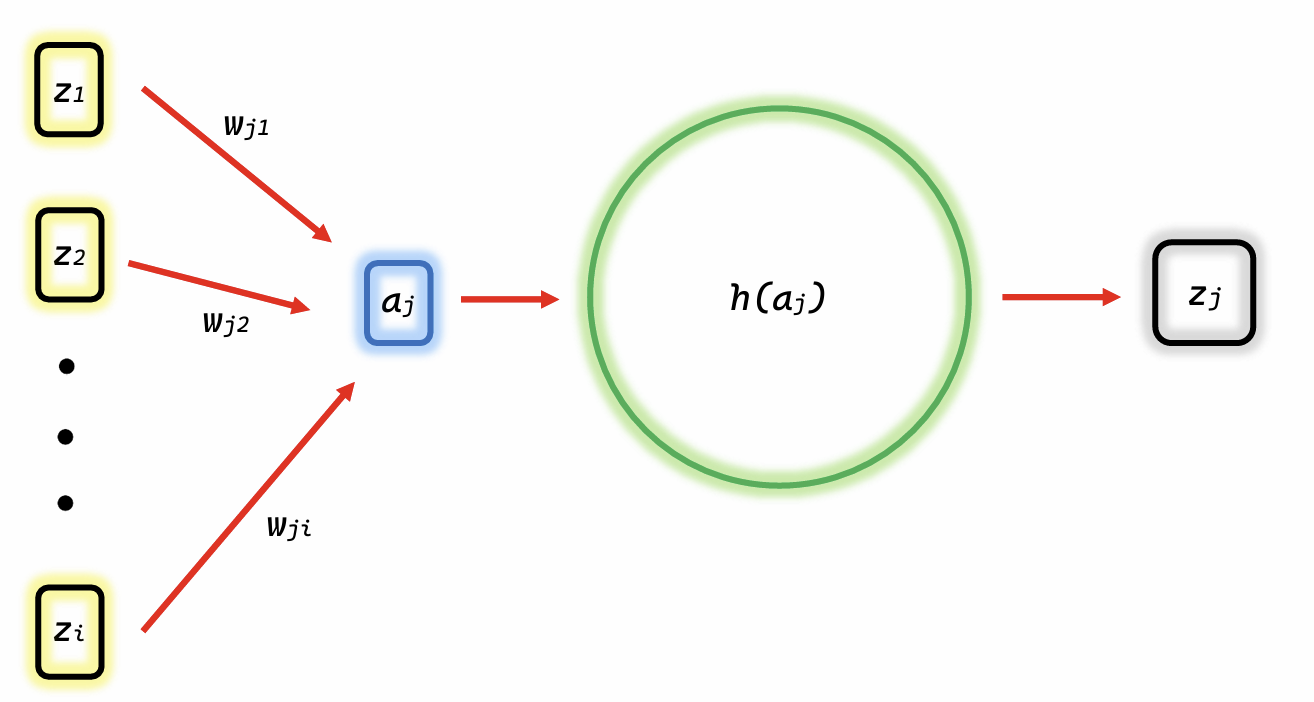
\includegraphics[scale=0.7]{imgss221.png}
	\caption{Representación de la operación de un nodo individual}
	\label{fig:figura70010As}
\end{figure}

La correcta aplicación de las ecuaciones (\ref{eq:ecuacion740}) y (\ref{eq:ecuacion741}) para cada vector de características significa el haber calculado todas las combinaciones lineales y señales de salida de cada uno de 
los nodos de la capa de salida y todas las capas ocultas presentes. Ahora consideremos la derivada de \textit{$E_n$} con respecto a un peso cualquiera; el error \textit{$E_n$} depende siempre del peso de enlace previo a través 
de la activación \textit{$a_j$} que es entrada al j-ésimo nodo. Dado lo anterior sobre la dependencia de \textit{$E_n$} con el peso de enlace previo y entrada de activación previa, al aplicar la derivada se puede hacer uso de 
la regla cadena para generar la ecuación (\ref{eq:ecuacion742}).

\begin{equation}
	\frac{\partial{E_n (w_{ji})}}{\partial{w_{ji}}}=\frac{\partial{E_n}}{\partial{a_{j}}} \frac{\partial{a_j}}{\partial{w_{ji}}}
	\label{eq:ecuacion742}
\end{equation}

Haciendo un cambio de notación dado por (\ref{eq:ecuacion743}).

\begin{equation}
	\delta_{j}=\frac{\partial{E_n}}{\partial{a_{j}}}
	\label{eq:ecuacion743}
\end{equation}

Si la ecuación (\ref{eq:ecuacion740}) la derivamos con respecto de un peso cualquiera, nos queda el dato de entrada de la combinación lineal que no depende del valor del peso, por lo tanto resulta la expresión (\ref{eq:ecuacion744}).

\begin{equation}
	\frac{\partial{a_j}}{\partial{w_{ji}}}=z_i
	\label{eq:ecuacion744}
\end{equation}

Ahora sustituyendo las ecuaciones (\ref{eq:ecuacion743}) y (\ref{eq:ecuacion744}) en la ecuación (\ref{eq:ecuacion742}), obtenemos la expresión simplificada (\ref{eq:ecuacion745}).

\begin{equation}
	\frac{\partial{E_n}}{\partial{w_{ji}}}=\delta_{j} z_i
	\label{eq:ecuacion745}
\end{equation}

La ecuación (\ref{eq:ecuacion745}) nos dice que la derivada del error respecto a un peso cualquiera se obtiene al multiplicar el error parcial \textit{$\delta$} en el extremo de salida de un nodo \textit{ji}, por la activación de entrada 
en el extremo del inicio del enlace entre nodos. Por lo cual, para calcular las derivadas es necesario obtener los valores $\delta$ para cada nodo de las capas ocultas y de salida, y posteriormente aplicar la ecuación (\ref{eq:ecuacion745}).

Para los nodos de la capa de salida ya se conoce la relación dada por (\ref{eq:ecuacion746}) para el error en el k-ésimo nodo.

\begin{equation}
	\delta_{k}=y_{k} - t_k
	\label{eq:ecuacion746}
\end{equation}

Para los nodos de las capas ocultas, el cálculo de los valores $\delta$ para cada capa implica volver a aplicar la regla de la cadena (\ref{eq:ecuacion747})

\begin{equation}
	\delta_{j}=\frac{\partial{E_n}}{\partial{a_{j}}}=\sum_{k}^{} {\frac{\partial{E_n}}{\partial{a_{k}}} \frac{\partial{a_k}}{\partial{a_{j}}}}
	\label{eq:ecuacion747}
\end{equation}

donde la sumatoria se aplica sobre todos los nodos de la k-ésima capa a los cuales un nodo de la j-ésima capa previa envía una conexión sináptica. Cuando se habla de k-ésima capa se hace referencia a que esta capa puede ser 
capa de salida o capa oculta. Si en la ecuación (\ref{eq:ecuacion747}) se usa (\ref{eq:ecuacion743}) para hacer la substitución de la derivada parcial del error por el valor $\delta$ y posteriormente 
se usan las ecuaciones (\ref{eq:ecuacion740}) y (\ref{eq:ecuacion741}) para sustituir por la derivada parcial de la k-ésima entrada de activación, se puede llegar a una ecuación general de propagación hacia atrás del error.

\begin{equation}
	\delta_{k}=\frac{\partial{E_n}}{\partial{a_{k}}}
	\label{eq:ecuacion748}
\end{equation}

\begin{equation}
	\frac{\partial{a_k}}{\partial{a_{j}}}=\frac{\partial{\sum_{k}^{} {w_{kj} z_j}}}{\partial{a_{j}}}
	\label{eq:ecuacion749}
\end{equation}

Desarrollando (\ref{eq:ecuacion749})

\begin{equation}
	\frac{\partial{a_k}}{\partial{a_{j}}}=\frac{\partial{\sum_{k}^{} {w_{kj} h(a_j)}}}{\partial{a_{j}}}
	\label{eq:ecuacion750}
\end{equation}

La derivada puede introducirse en la sumatoria

\begin{equation}
	\frac{\partial{a_k}}{\partial{a_{j}}}=\sum_{k}^{} {\frac{\partial{w_{kj} h(a_j)}}{\partial{a_{j}}}}
	\label{eq:ecuacion751}
\end{equation}

El peso \textit{w} al no depender de \textit{$a_j$} puede salir de la derivada

\begin{equation}
	\frac{\partial{a_k}}{\partial{a_{j}}}=\sum_{k}^{} {w_{kj} \frac{\partial{h(a_j)}}{\partial{a_{j}}}}
	\label{eq:ecuacion752}
\end{equation}

La derivada, al no tener dependencia sobre el subíndice \textit{k}, puede salir de la sumatoria 

\begin{equation}
	\frac{\partial{a_k}}{\partial{a_{j}}}=\frac{\partial{h(a_j)}}{\partial{a_{j}}} \sum_{k}^{} {w_{kj}} 
	\label{eq:ecuacion753}
\end{equation}

Finalmente, sustituyendo los resultados (\ref{eq:ecuacion753}) y (\ref{eq:ecuacion748}) en la ecuación (\ref{eq:ecuacion747}) se llega al resultado (\ref{eq:ecuacion754})

\begin{equation}
	\delta_{j}=\frac{\partial{h(a_j)}}{\partial{a_{j}}} \sum_{k}^{} {w_{kj} \delta_{k}} 
	\label{eq:ecuacion754}
\end{equation}

%La ecuación (\ref{eq:ecuacion754}) representa un método general para la propagación hacia atrás del error en una red neuronal y nos dice que el error parcial en un nodo de una capa oculta se puede obtener al propagar hacia 
%atrás los errores de capas posteriores. Por lo tanto los pasos a seguir para el ajuste de una red neuronal son los siguientes:

La ecuación (\ref{eq:ecuacion754}) representa una expresión general para el cálculo de los errores proporcionales para las capas ocultas. Este resultado nos permite el uso de la ecuación (\ref{eq:ecuacion745}) para el cálculo 
de las derivadas del error con respecto a los pesos correspondientes, lo cual es requerido para la ecuación de Newton-Raphson para actualización de los pesos. 

Por último, se debe señalar que en la ecuación (\ref{eq:ecuacion754}), al ser una forma general, ya en la práctica se debe tener en cuenta que diferentes capas de la red neuronal pueden tener diferentes funciones de activación, 
por lo cual al usar dicha ecuación debe usarse la correspondiente función de activación que exista en la capa de la red donde se estén realizando los ajustes.

De forma general, el procedimiento para el ajuste de una red neuronal es el siguiente:

\begin{lstlisting}[language=Python,numbers=none]
	DEFINIR NUMERO DE ENTRADAS 
	input_nodes:A

	DEFINIR NUMERO DE SALIDAS
	output_nodes:B

	DEFINIR CAPAS OCULTAS
	hidden_nodes:C

	INICIALIZAR PESOS DE LA RED CON DISTRIBUCION NORMAL COMO REFERENCIA
	wih:numpy.random.normal(0.0,pow(self.inodes,-0.5),(self.hnodes,self.inodes))
	who:numpy.random.normal(0.0,pow(self.hnodes,-0.5),(self.onodes,self.hnodes))

	DEFINIR LA TASA DE APRENDIZAJE
	lr:learningrate

	PROPAGACION HACIA ADELANTE
	hidden_inputs:numpy.dot(wih,inputs)
	hidden_outputs:self.activation_function(hidden_inputs)
	final_inputs:numpy.dot(who,hidden_outputs)
	final_outputs:self.activation_function(final_inputs)

	PROPAGACION HACIA ATRAS DEL ERROR
	output_errors:targets-final_outputs
	hidden_errors:numpy.dot(who.T,output_errors)

	ACTUALIZAR LOS PESOS
	who:who+lr*numpy.dot((output_errors*final_outputs*(1-final_outputs)),numpy.transpose(hidden_outputs))
	wih:wih+lr*numpy.dot((hidden_errors*hidden_outputs*(1-hidden_outputs)),numpy.transpose(inputs))
\end{lstlisting}

Primero es necesario definir la arquitectura de la red al establecer las capas y la cantidad de nodos en ellas. Después, se debe inicializar de forma aleatoria los pesos entre capa de entrada y capa oculta, los pesos entre 
capas ocultas y los pesos entre capa oculta y capa de salida. Al mismo tiempo es necesario establecer la tasa de aprendizaje con la cual se optimizará el modelo.

Posteriormente, se deben propagar por la red los datos de entrenamiento para obtener las estimaciones hechas con el valor actual de pesos. Finalmente, se debe hacer el cálculo de los errores en la salida de la red y los 
errores proporcionales para los pesos de capas intermedias. Con esta información se puede generar actualizaciones secuenciales sobre los pesos de la red. 

\section{Conclusiones}

En este capítulo se presentan los conceptos y desarrollo matemático para los diferentes algoritmos de inteligencia artificial que son parte del desarrollo de este trabajo. Primeramente se inicia con los conceptos fundamentales 
acerca de la regresión lineal, el cual es un método que nos permite obtener funciones matemáticas, dadas por un recta, para representar un patrón o comportamiento dado por un conjunto de datos.

Con los conceptos introducidos en las secciones dedicadas a regresión lineal, es que se identifica la necesidad de contar con métodos de ajuste para los parámetros de un modelo en específico, con el fin de obtener la mejor 
optimización. Es aquí donde se introduce el método de descenso por gradiente para minimización de una función de error dependiente de los parámetros del modelo aplicado. Este método de ajuste iterativo permite ejecutar cambios 
graduales en los parámetros del modelo utilizado hasta llegar a la mejor aproximación para el mínimo de la función de error.

Posteriormente, se desarrollan los conceptos básicos para modelos no lineales para clasificación, para después pasar con el caso específico empleado en este trabajo, que son las redes neuronales. En esta parte se explican 
las analogías entre una red biológica y una artificial, y como se van generando las ecuaciones matemáticas para nodos o neuronas individuales en la red, para posteriormente poder apilar o conjuntar nodos mediante enlaces 
por pesos para nodos de capas consecutivas en la red.

Por último, se describe un enfoque generalizado para el entrenamiento de la red neuronal artificial, describiendo mediante ecuaciones los procedimientos de propagación hacia adelante de los datos de entrenamiento y después 
la propagación hacia atrás del error a la salida del modelo, para finalmente usar la información obtenida mediante esta realimentación del error para poder hacer modificaciones en los enlaces o pesos que forman la red neuronal.

% TERMINADO YA ESTE CAPÍTULO.

\cleardoublepage
\chapter{Materiales y Métodos}
\label{ch:Instrumentacion}

Toda la información presentada en este capítulo es obtenida de los manuales de referencia del fabricante de equipos de medición Atlas Scientific, así como las imágenes de referencia presentadas también son extraídas de 
dichos manuales u hojas de datos, así como del sitio web del fabricante, https://atlas-scientific.com/.

\section{Medición de Temperatura}

%\subsection{Sonda de Temperatura PT-1000}

La \autoref{fig:figura500_1} muestra la sonda de temperatura PT-1000 utilizada para la recolección de datos de la variable de temperatura.

\begin{figure}[h]
	\centering
	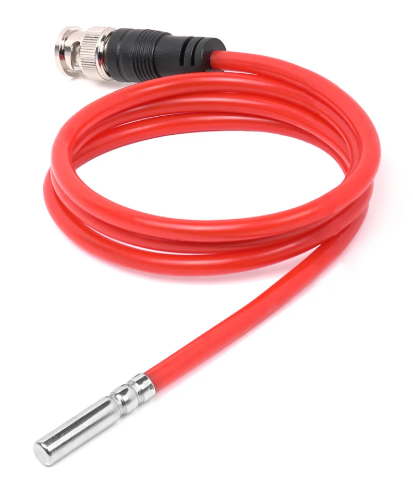
\includegraphics[scale=0.5]{imgss110.png}
	\caption{Sonda PT-1000. Imagen obtenida del manual \textit{Atlas Scientific. PT-1000 Temperature Probe}}
	\label{fig:figura500_1}
\end{figure}

\clearpage

Las principales características de este instrumento se presentan en el siguiente listado:

\begin{itemize}
    \item El transductor te temperatura utilizado por esta sonda es una RTD (Resistance Temperature Detector, Detector de Temperatura Resistivo), cuyo material de fabricación es Platino de Clase A de alta pureza.
    \item Su rango de medición abarca desde los -200°C hasta los 850°C 
    \item Posee una exactitud de +/-(0.15+(0.002t)), donde t es el valor de temperatura medido.
    \item Tipo de conector BNC (Bayonet Neill-Concelman) para transmisión de la señal detectada en el medio donde se mide la temperatura.
    \item Expectativa de vida útil de 15 años.
    \item Material de caucho de silocona utilizado en la manguera que une al conector BNC con el transductor.
    \item Capacidad de sumergir por tiempo indefinido la totalidad de la sonda en agua dulce o salada.
    \item La limpieza del instrumento consiste en cepillar de forma suave la punta metálica para remover los residuos que pudiesen formarse con el paso del tiempo.  
\end{itemize}


Las aplicaciones típicas del instrumento se enlistan a continuación:

\begin{itemize}
    \item Uso estándar para análisis de laboratorio.
    \item Uso en suelo o tierra en prácticas de campo.
    \item Capacidad de sumergirse en una amplia variedad de líquidos, con excepción de aquellos que pudiesen dañar el material de la punta metálica o la manguera.
    \item Elegible para comunicación de los datos recolectados con los kits Hydroponics y Aquaponics de Atlas Scientific.
\end{itemize}

\subsection{Principio de Funcionamiento de la Sonda PT-1000}

En las operaciones de medición de temperatura, existen diversos materiales usados en los transductores especializados para este parámetro; algunos de los más utilizados son el níquel, el cobre y el platino. De estos 3 materiales
mencionados, el platino es el elegido ampliamente como estándar industrial para medición de temperatura contra otros materiales. La razón de esta elección es la relación de linealidad entre la resistencia o impedancia del 
material y la temperatura a la cual se encuentra. Es decir, por ejemplo para materiales como el níquel o el cobre, una gráfica de la relación entre la temperatura de dichos materiales y la impedanacia que presentan a dicha 
temperatura, resulta una relación matemática no lineal. En cambio, si el material elegido es el platino, la relación matématica entre impedancia del material y su temperatura resulta en una aproximación cercana a ser lineal. Para 
casos como este, resulta altamente preferible el uso de un material que tenga una relación que se aproxime a ser lineal, ya que esto simplifica los cálculos para valores de temperatura con base en los valores de impedancia que presenta
el transductor, en este caso de platino.

El nombre PT-1000 de la sonda hace referencia al elemento Platino mediante las letras PT, y el número 1000 se relaciona con el valor de resistencia de 1000 ohms medido en el material a una temperatura de 0°C. El cálculo de la 
temperatura con respecto a la resistencia presentada por el Platino tiene la forma (\ref{eq:ecuacion501})

\begin{equation}
	T(R)=\frac{3.908-\sqrt{17.59246-0.00232R}}{0.00116}
	\label{eq:ecuacion501}
\end{equation}

Como ya se ha mencionado, el valor de \textit{R} es la resistencia medida en el Platino en la sonda y \textit{T(R)} es la temperatura en función de la resistencia \textit{R}, expresada en grados Celsius.

\section{Medición de Potencial de Hidrógeno (pH)}

La \autoref{fig:figura500_2} muestra la sonda \textit{Consumer Grade} utilizada para la recolección de datos de la variable de pH.

\begin{figure}[h]
	\centering
	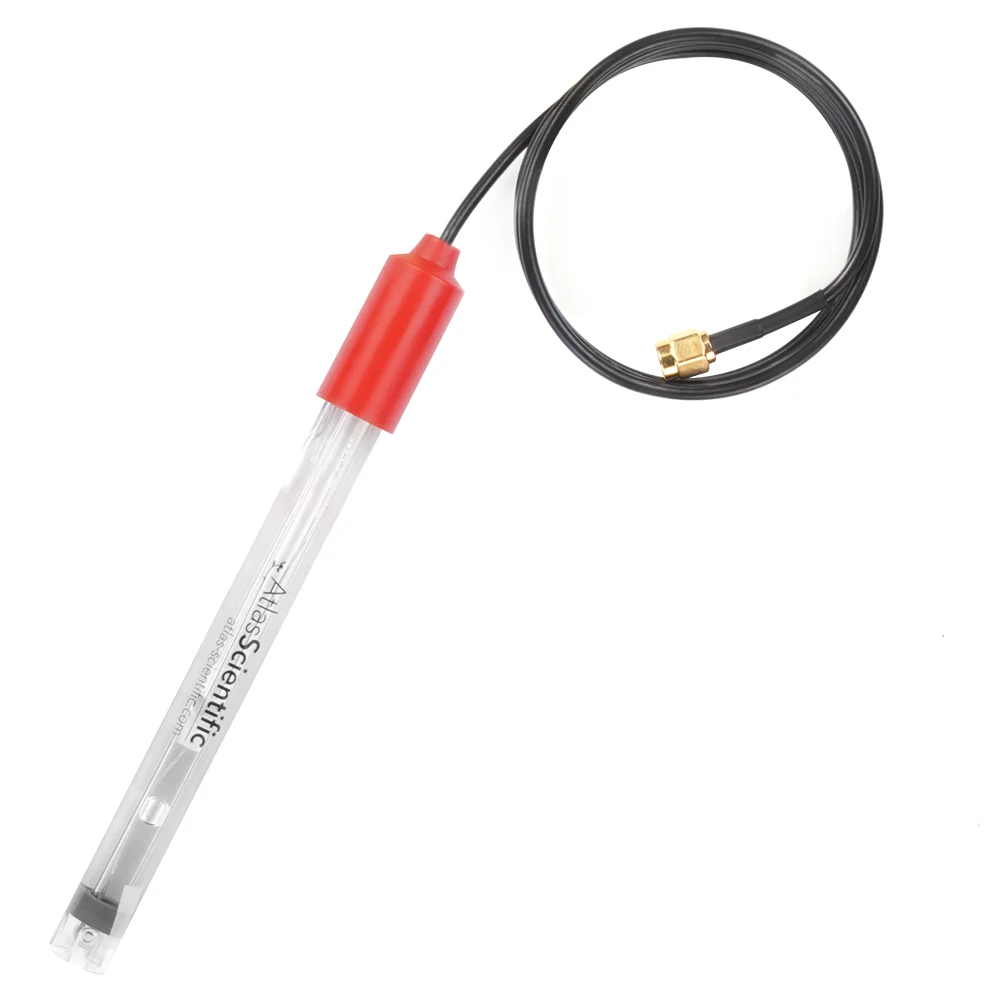
\includegraphics[scale=0.2]{imgss111.png}
	\caption{Sonda Consumer Grade para medición de pH. Imagen obtenida del manual \textit{Atlas Scientific. Consumer Grade pH Probe}}
	\label{fig:figura500_2}
\end{figure}

Sus principales características se enlistan a continuación:

\begin{itemize}
    \item Rango de medición de 2 a 13 en la escala estandarizada.
    \item Resolución en la medición de +/-(0.1).
    \item Precisión en la medición de +/-(0.1).
    \item Rango de temperatura de funcionamiento de 1°C a 60°C.
    \item Capacidad de soportar hasta 50PSI de presión en operación.
    \item Profundidad sumergible máxima de 35m; primeramente es necesario ampliar la longitud del cable de la sonda mediante cables externos compatibles.
    \item Tipo de conector SMA (SubMiniature Version A). Configurable para conector BNC mediante adaptadores externos.
    \item No disponible con sensor interno de temperatura.
    \item Capacidad de uso continuo durante 3 meses antes de requerir calibración.
    \item Expectativa de vida útil del sensor de 12 a 18 meses.
    \item Electrodo de referencia fabricado en plata/cloruro de plata (Ag/AgCl).
    \item Las sondas de medición de pH deben permanecer mojadas y no dejar que se seque la parte sensitiva del instrumento cuando éste no se encuentre en operación. El procedimiento estándar para mantener la sonda cuando no está 
    en funcionamiento es introducir la punta sensitiva de la sonda en el frasco con solución de almacenamiento incluida para este tipo de instrumento.
    \item Si la sonda es utilizada para medición en medios donde se estén llevando a cabo procesos químicos, procesos industriales o donde se tenga la presencia de soluciones con ácidos o bases altamente concentrados, es 
    necesario llevar a cabo la calibración del instrumento de forma más frecuente. Preferentemente, al menos 2 veces al mes o mayor número de veces si el uso del instrumento es en soluciones con alta concentración.    
\end{itemize}

Las aplicaciones típicas de la sonda de pH se enlistan a continuación:

\begin{itemize}
    \item Uso en pruebas de laboratorio.
    \item Uso en pruebas de campo.
    \item Medición de pH en diversos tipos de suelo.
    \item Medición en soluciones que contengan metales pesados.
    \item Elegible para comunicación de los datos recolectados con los kits Hydroponics y Aquaponics de Atlas Scientific.
\end{itemize}

\subsection{Principio de Funcionamiento de la Sonda de pH}

Una sonda de pH se encarga de medir el nivel de actividad de los iones (cationes) de Hidrógeno en un líquido.

La punta de la sonda contiene una membrana de cristal, la cual permite el paso de una cierta cantidad de cationes Hidrógeno al interior de la membrana, mientras los iones restantes permanecen en la solución que se está midiendo. 
La diferencia en la concentración de los cationes que están dentro de la membrana contra la concentración de los cationes que quedan fuera, genera una diferencia de potencial eléctrico el cual da origen a una pequeña corriente 
eléctrica. La magnitud de dicha corriente resulta proporcional al nivel de concentración de iones Hidrógeno en el líquido medido.

Específicamente, cuando la concentración de cationes Hidrógeno dentro de la membrana es menor a la concentración de los que quedan fuera, se tiene un valor de pH menor a 7, es decir, ácido. En el caso contrario, cuando la 
concentración de cationes es mayor dentro de la membrana, el pH tendrá un valor mayor a 7, es decir, alcalino. El último caso se presenta cuando la concentración de cationes dentro de la membrana es igual a la concentración 
fuera de ella; en este caso, el pH es de 7, es decir, neutro.

En la \autoref{fig:figura15856} se muestra una imagen de la escala estándar del parámetro pH.

\clearpage

\begin{figure}[h]
	\centering
	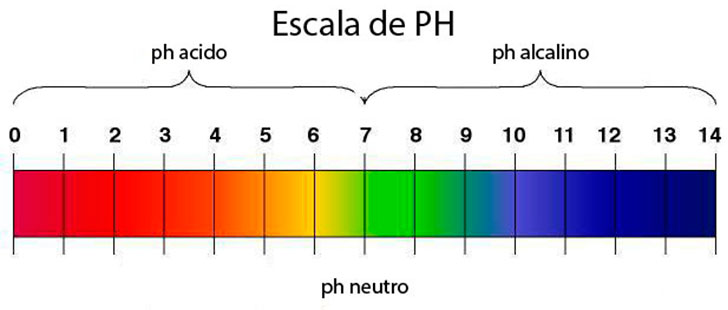
\includegraphics[scale=0.6]{imgss204.jpg}
	\caption{Escala estándar para magnitud de pH. Imagen obtenida de fuentes de internet}
	\label{fig:figura15856}
\end{figure}

\section{Medición de Potencial de Óxido-Reducción (ORP)}

La \autoref{fig:figura500_3} muestra la sonda \textit{Consumer Grade} utilizada para la recolección de datos de la variable de ORP.

\begin{figure}[h]
	\centering
	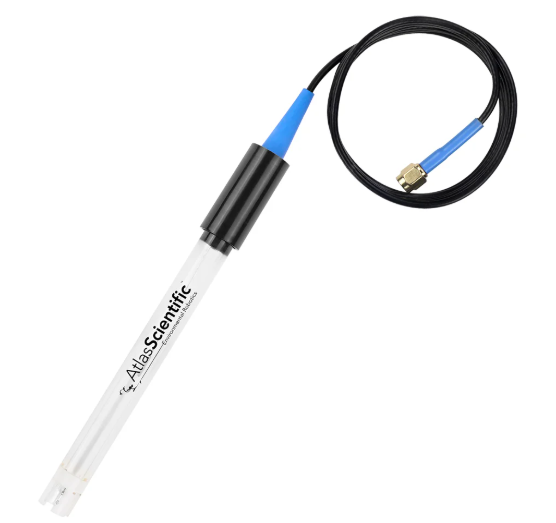
\includegraphics[scale=0.6]{imgss112.png}
	\caption{Sonda Consumer Grade para medición de ORP. Imagen obtenida del manual \textit{Atlas Scientific. Consumer Grade ORP Probe}}
	\label{fig:figura500_3}
\end{figure}

Sus principales características se enlistan a continuación:

\begin{itemize}
    \item Rango de medición de -1100mV a 1100mV.
    \item Exactitud de +/-(1.1mV).
    \item Rango de temperatura de operación de 1°C a 60°C.
    \item Capacidad de soportar hasta 50PSI de presión en operación.
    \item No recomendada para la medición en ácidos o bases fuertes, ni tampoco en procesos industriales. 
    \item Profundidad sumergible máxima de 35m; primeramente es necesario ampliar la longitud del cable de la sonda mediante cables externos compatibles.
    \item Tipo de conector SMA. Configurable para conector BNC mediante adaptadores externos.
    \item No disponible con sensor interno para medición de temperatura.
    \item Periodo de tiempo aproximado de 3 meses antes de requerir recalibración.
    \item Expectativa de vida útil aproximada del sensor de 12 a 18 meses.
    \item Cuando la sonda no está en uso, su almacenamiento debe ser introduciendo la punta metálica de platino en la solución para conservación incluida con el instrumento.
    \item Si el uso de la sonda es en medios donde se llevan a cabo reacciones químicas agresivas, es recomendable realizar la calibración de la sonda antes de cada uso.
    \item Si a la sonda al estar almacenda la punta metálica de platino en su solución para conservación, se le llegasen a formar residuos blancos en el tubo de cristal, dichos residuos son Cloruro de Potasio (\textit{KCl}). Antes de 
    volver a usar la sonda, enjuagarla con agua destilada hasta retirar todos los residuos. 
\end{itemize}

Las aplicaciones típicas del instrumento se enlistan a continuación:

\begin{itemize}
    \item Uso en pruebas de laboratorio.
    \item Uso en pruebas de campo.
    \item Medición en soluciones que contengan metales pesados.
    \item Elegible para comunicación de los datos recolectados con los kits Hydroponics y Aquaponics de Atlas Scientific.
\end{itemize}

\subsection{Principio de Funcionamiento de la Sonda de ORP}

Una sonda de ORP tiene como propósito medir o detectar la actividad de los electrones presentes en un líquido.

Las mediciones del parámetro de ORP representan qué tan fuerte es la transferencia de electrones a una sustancia o desde una sustancia en un líquido. Resaltando que la medición de ORP no tiene relación con la cantidad de 
electrones disponible en el líquido para una transferencia de cargas entre diferentes sustancias. Por lo tanto, expresado de otra forma, un transductor de ORP lo que hace es detectar la pequeña corriente eléctrica generada 
en el agua cuando existe un fenómeno de oxidación o reducción de otra sustancia en dicho líquido.

La sonda de ORP de Atlas Scientific está integrada por una punta metálica de platino, la cual se encuentra conectada a un conductor de plata, rodeado o inmerso en el compuesto Cloruro de Plata (AgCl). Adicionalmente, este 
conductor de plata se encuentra en contacto con una sustancia de referencia de Cloruro de Potasio (KCl). El material de platino en la punta metálica de la sonda es usado debido a que este metal se mantiene inactivo cuando se 
introduce en un líquido para realizar mediciones, es decir, dicho material se mantiene al margen de cualquier actividad electrónica que pudiése estar ocurriendo en el líquido.

\clearpage

\section{Medición de Conductividad Eléctrica}

La \autoref{fig:figura500_4} muestra la sonda \textit{K 0.1} utilizada para la recolección de datos de la variable de conductividad eléctrica.

\begin{figure}[h]
	\centering
	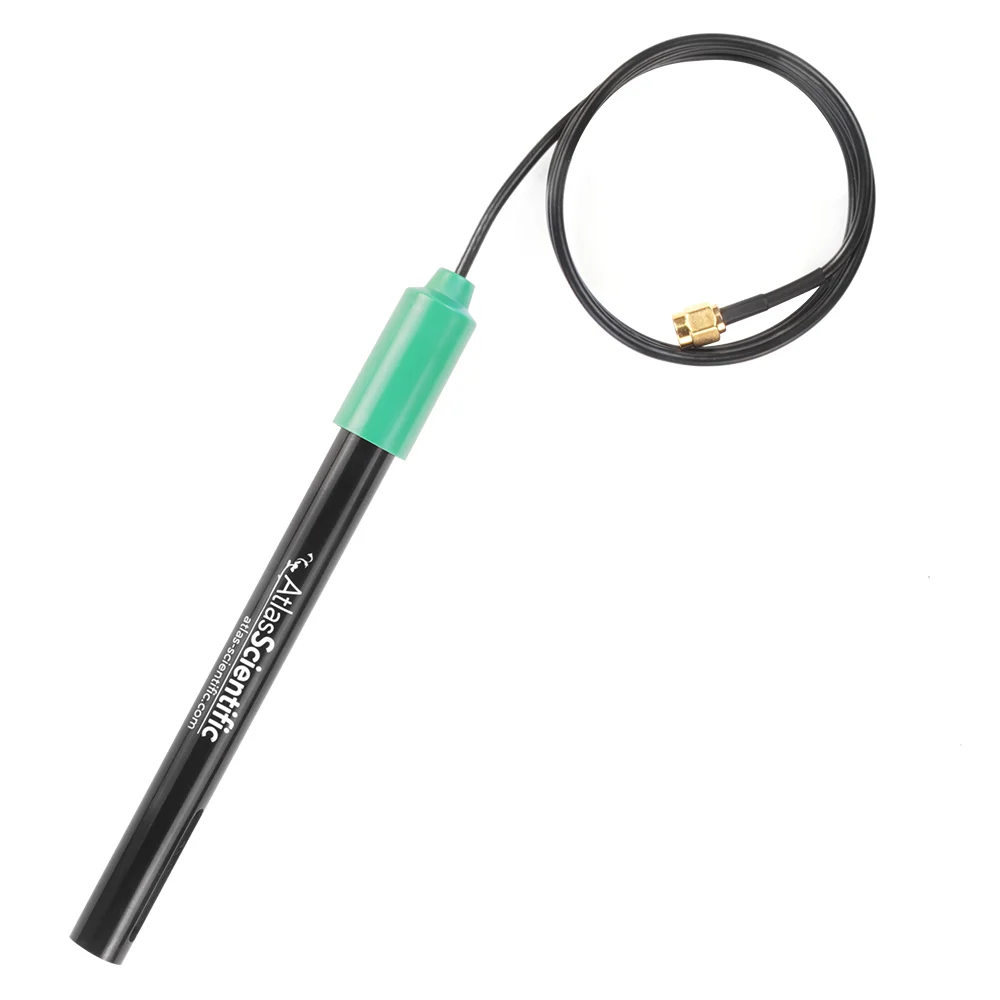
\includegraphics[scale=0.2]{imgss113.png}
	\caption{Sonda K 0.1 de medición de electroconductividad. Imagen obtenida del manual \textit{Atlas Scientific. Conductivity Probe K 0.1}}
	\label{fig:figura500_4}
\end{figure}

Sus principales características se enlistan a continuación:

\begin{itemize}
    \item Rango de medición de 0.07$\mu$S/cm a 50000$\mu$S/cm.
    \item Exactitud de +/-(2\%)
    \item Rango de temperatura de operación de 1°C a 110°C.
    \item Capacidad de soportar hasta 500PSI de presión en operación.
    \item Profundidad sumergible máxima de 352m; primeramente es necesario ampliar la longitud del cable de la sonda mediante cables externos compatibles.
    \item Tipo de conector SMA. Configurable para conector BNC mediante adaptadores externos.
    \item No disponible con sensor interno de temperatura.
    \item Expectativa de vida útil aproximada del sensor de 10 años.
    \item Superficie sensitiva de medición fabricada en material Grafito.
    \item Sumergible tanto en agua dulce como agua salada.
    \item La sonda K 0.1 trabaja al medir la corriente eléctrica generada en el agua entre sus 2 placas de grafito. Mientras dichas placas no se dañen ni tengan que ser reemplazadas, no es necesario realizar recalibración, 
    es decir, la primera calibración realizada antes de su primer uso es la única indispensable. 
\end{itemize}

Las aplicaciones típicas de este instrumento se enlistan a continuación:

\begin{itemize}
    \item Uso en pruebas de laboratorio.
    \item Uso en prácticas de campo.
    \item Medición en acuarios o pesceras.
    \item Elegible para comunicación de los datos recolectados con los kits Hydroponics y Aquaponics de Atlas Scientific.
    \item Medición en mezclas acuosa/orgánica.
    \item Medición en líquidos con presencia de metales pesados.
    \item Muestreo en suelos húmedos.
    \item Medición en sustancias o agentes reductores fuertes.
\end{itemize}

\subsection{Principio de Funcionamiento de la Sonda K 0.1}

La sonda K 0.1 de Atlas Scientific se encarga de realizar mediciones de la conductividad eléctrica en la solución líquida donde se sumerge. Las mediciones de conductividad en líquidos generalmente tiene como propósito el conocer 
la concentración de sales, nutrientes o impurezas.

Dentro de la sonda K 0.1, se encuentran 2 electrodos posicionados de forma opuesta uno del otro. Dada esta configuración, una vez que la sonda es sumergida en el líquido a ser analizado, un voltaje es aplicado entre dichos 
electrodos ocasionando que los cationes presentes en el líquido se desplazen hacia el electrodo polarizado con carga negativa, mientras que los aniones que se encuentren en el líquido se desplazarán hacia el electrodo que presenta
carga neta positiva. Por lo tanto, entre mayor sea la concentración de iones en el líquido analizado, mayor será la corriente generada entre los electrodos.

Es muy importante que al momento de realizar mediciones con la sonda K 0.1, el usuario continuamente verifique que no se formen burbujas entre las 2 celdas o electrodos, ya que este fenómeno afectará considerablemente los valores 
medidos. Cuando dicho fenémeno se presente, es necesario que el usuario genere sobre la sonda pequeños golpes para retirar los cúmulos de burbuja que pudieran estar presentes.

Con el paso del tiempo y el uso del instrumento, es probable que exista la formación de residuos en las áreas sensibles de la sonda, lo cual podría afectar las propiedades eléctricas de las celdas o electrodos y generar mediciones 
erróneas. Por lo cual es necesario que el usuario haga uso de un cepillo de cerdas suaves para remover dichos residuos.


\clearpage

\section{Medición de Oxígeno Disuelto}

La \autoref{fig:figura500_5} muestra la sonda \textit{Lab Grade} utilizada para la recolección de datos para el parámetro de Oxígeno Disuelto.

\begin{figure}[h]
	\centering
	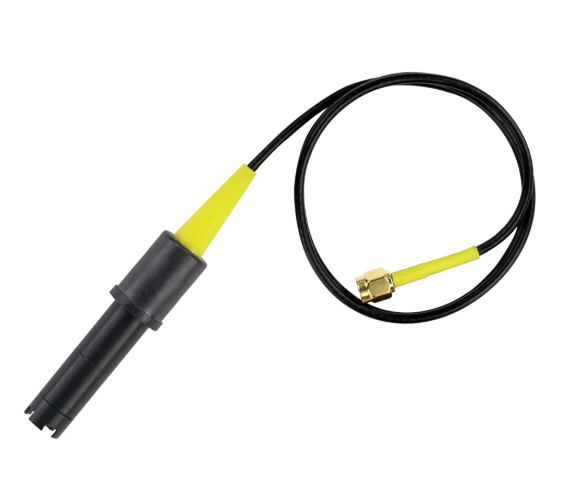
\includegraphics[scale=0.6]{imgss114.png}
	\caption{Sonda Lab Grade para Oxígeno Disuelto. Imagen obtenida del manual \textit{Atlas Scientific. Lab Grade D.O. Probe}}
	\label{fig:figura500_5}
\end{figure}

Sus principales características se enlistan a continuación:

\begin{itemize}
    \item Rango de medición de 0mg/L a 100mg/L.
    \item Exactitud de +/-(0.05mg/L).
    \item Rango de temperatura de operación de 0°C a 60°C.
    \item Capacidad de soportar hasta 500PSI de presión en operación.
    \item Profundidad sumergible máxima de 352m; primeramente es necesario ampliar la longitud del cable de la sonda mediante cables externos compatibles.
    \item Tipo de conector SMA. Configurable para conector BNC mediante adaptadores externos.
    \item No disponible con sensor interno de temperatura.
    \item Periodo de tiempo aproximado de 1 año antes de requerir recalibración.
    \item Expectativa de vida útil aproximada del sensor de 4 años.
    \item Sumergible en agua dulce o salada.
\end{itemize}

\clearpage

Las aplicaciones típicas de la sonda Lab Grade son las siguientes:

\begin{itemize}
    \item Uso en pruebas de laboratorio.
    \item Uso en pruebas de campo.
    \item Uso en actividades de cuidado y preservación de especies acuáticas.
    \item Uso en producción de vino.
    \item Uso para monitoreo de condiciones ambientales.
\end{itemize}

\subsection{Principio de Funcionamiento de la Sonda Lab Grade}

La sonda Lab Grade de Atlas Scientific es una sonda galvánica para medición de Oxígeno Disuelto que consiste de una membrana de tipo PTFE (Politetrafluoroetileno), un ánodo bañado o inmerso en electrolito y su cátodo correspondiente.
Cuando la sonda es sumergida en el líquido analizado, las moléculas de oxígeno se difunden a través de la membrana; cuando ha ocurrido lo anterior, las moléculas de oxígeno son reducidas por medio del cátodo, generando una 
pequeña diferencia de potencial eléctrico. En caso de no haber moléculas de oxígeno presentes, la sonda entregará una señal eléctrica de 0V. Es decir, entre mayor sea la concentración de moléculas de oxígeno presentes, mayor 
será la señal en milivoltios entregada por el instrumento.

Importante resaltar que esta sonda galvánica en específico tiene la capacidad de entregar una señal en el rango de 0mV a 60mV, dependiendo de la saturación de oxígeno dentro de la membrana.

Con el uso continuo de la sonda, es probable que alrededor de la zona sensitiva del instrumento se formen residuos de cloruro de potasio (KCl) provenientes del electrolito del interior. Cuando esto ocurra, es necesario enjuagar 
con agua destilada la zona afectada por los residuos hasta que quede libre de ellos. Finalmente, muy importante que si los residuos se forman directamente en la zona de la membrana sensitiva, bajo ninguna circunstancia se debe 
cepillar la zona para retirarlos, ya que esto dañara la membrana y las mediciones comenzarán a ser erróneas. En este caso, es recomendable usar detergente líquido para enjuagar la zona hasta retirar los residuos acumulados.

\clearpage

\section{Equipo Wi-Fi Pool Kit de Atlas Scientific}

La \autoref{fig:figura500_6} muestra una imagen del equipo. Externamente la caja contiene en la parte frontal 4 conectores de tipo SMA, que permiten poder conectar 4 sondas de medición, dando de esta forma la posibilidad de medir el mismo tiempo 4 parámetros en la muestra de agua 
analizada. En la parte trasera, se tiene un conector USB Tipo B para la alimentación y comunicación por medio de una computadora externa. Internamente contiene 4 circuitos de instrumentación para acondicionamiento de las señales entregadas por las sondas en uso. Estas 4 tarjetas PCB envían los datos previamente procesados a un microcontrolador ESP32.

\begin{figure}[h]
	\centering
	\includegraphics[scale=0.05]{imgss203.jpg}
	\caption{Wi-Fi Pool Kit.}
	\label{fig:figura500_6}
\end{figure}

La metodología utilizada para trabajar con este equipo consiste primeramente en la recolección de las muestras de agua que serán caracterizadas. Una vez que las muestras se tienen disponibles en frascos de muestreo, se sumergen 
en ella 4 sondas de los parámetros deseados, las cuales también son conectadas a los puertos SMA. Una vez que se tiene dicha configuración, el kit debe conectarse a una computadora para iniciar la comunicación con el 
microcontrolador ESP32, el cual está recibiendo secuencialmente un registro de 4 datos correspondiente a las 4 sondas utilizadas. Este registro de 4 valores numéricos es posible imprimirlos en la terminal del IDE de Arduino,
para posteriormente exportar dichos registros a un archivo CSV. externo donde quedarán almacenados todos los registros recolectados, para su posterior uso para análisis de estadística descriptiva y tareas de entrenamiento y 
validación en modelos clasificadores para estimación de Calidad del Agua.

Las principales prestaciones del kit Wi-Fi Pool se detallan a continuación.

\begin{itemize}
    \item El equipo viene configurado de fabrica para realizar la medición de los parámetros de temperatura, pH y ORP; el cuarto puerto disponible auxiliar está disponible para la conexión de otro circuito de acondicionamiento 
    de señal para el monitoreo del cuarto y último parámetro disponible para este equipo.
    \item El equipo está diseñado para que el usuario pueda modificar sus funcionalidades. Es decir, el usuario puede cambiar tarjetas de acondicionamiento de señal disponibles por otras diferentes para otros parámetros adicionales,
    de acuerdo a las necesidades que se tengan.
    \item Equipo controlado mediante un microcontrolador ESP32, programable mediante la plataforma Arduino IDE.
    \item Los puertos de pH, ORP y el Auxiliar tienen aislamiento eléctrico; el puerto destinado para temperatura no dispone de dicha característica.
    \item El circuito requiere alimentación de 5V de CC en caso de no tener disponibilidad de conexión con una computadora, y se requiera alimentar mediante un adaptador o regulador externo.
    \item El microcontrolador ESP32 utiliza el protocolo I2C para comunicación con las tarjetas de acondicionamiento de señal. No es posible configurarlo para comunicación mediante protocolo UART en caso de ser 
    requerido por el usuario.
    \item Si el usuario requiere conectar diferentes tarjetas de acondicionamiento de señal a las ya incluidas, es necesario primero asegurarse que dichos circuitos previamente estén configurados para comunicación mediante 
    protocolo I2C.
    \item La interfaz de Arduino IDE permite la calibración de los circuitos de acondicionamiento de señal mediante el uso de comandos específicos desde la terminal del IDE.
\end{itemize}

\section{Calibración de los Sondas de Medición}

\subsection{Sonda de Temperatura}

Para realizar la calibración de la sonda de temperatura PT-1000 primeramente es necesario tener disponible un recipiente con agua hirviendo, la cual en teoría se encuentra a una temperatura de 100°C, sin embargo, el punto 
de ebullición del agua varía conforme la altura; a nivel del mar el punto de ebullición es de 100°C, y conforme la altura sobre el nivel del mar aumenta, el punto del ebullición del agua decrece un pequeño porcentaje.

Una vez que ya se tiene disponible el agua en su punto de ebullición, se debe conectar la sonda de temperatura al equipo Pool Kit en el conector correspondiente, y cargar al microcontrolador el código fuente disponible para 
descarga desde el sitio web de Atlas Scientific. Una vez que ya se tiene la conexión descrita, la punta de la sonda debe sumergirse en el agua hirviendo y posteriormente en la terminal del Arduino IDE, por comunicación serial, ejecutar el comando 
\textbf{rtd:cal,t}

\subsection{Sonda de pH}

Para la calibración de la sonda de pH se requiere de 3 soluciones de calibración específicas, para valor medio o neutro, valor bajo y valor alto. La solución de calibración de valor bajo contiene un compuesto a un pH de 
valor de 4, la solución de valor medio o neutro contiene un compuesto a un valor 7 de pH y la solución de valor alto contiene líquido de calibración a un valor 10 de pH.

Primeramente se debe tener conectada la sonda de pH al equipo Pool Kit en el conector correspondiente y el microcontrolador del equipo debe ejecutar el código fuente del fabricante Atlas Scientific. Una vez que se tiene 
listo lo descrito anteriormente, la sonda de pH debe introducirse en la solución de valor 7 de pH y esperar un rango de tiempo de 1 a 2 minutos mientras se estabilizan los valores medidos mostrados en la terminal del Arduino
IDE. Una vez que las lecturas mostradas en la terminal son estables, en terminal se debe ejecutar el comando \textbf{ph:cal,mid,7}; una vez terminado lo anterior, se tiene la sonda calibrada para valores neutros y la solución 
de calibración de valor 7 de pH debe desecharse ya que después de varios minutos de abierto el empaque, el líquido pierde sus propiedades. 

Finalmente, el proceso anterior debe repetirse para las soluciones de valor 4 y 10 de pH, las cuales requerirán los comandos \textbf{ph:cal,low,4} y \textbf{ph:cal,high,10}, respectivamente.

\subsection{Sonda de ORP}

El procedimiento para la calibración de la sonda de ORP consiste en el uso de la solución de calibración que proporciona el fabricante Atlas Scientific junto con el equipo Pool Kit. Primeramente es necesario tener la sonda 
de ORP conectada al equipo en su conector correspondiente y el microcontrolador ejecutando el código fuente desarrollado por el fabricante para este kit específico. Una vez que se tiene el equipo y la sonda en funcionamiento,
es necesario introducir la sonda dentro de la solución de calibración, la cual está diseñada para proveer un ORP con valor de 225mV. Una vez que se han estabilizado las lecturas impresas en la terminal del Arduino IDE, es 
necesario ejecutar el comando \textbf{orp:cal,225} con el cual el circuito quedará calibrado teniendo como referencia este valor dado por esta solución específica.

En caso de que el usuario tenga a su disposición una solución de calibración diferente a la del fabricante Atlas Scientific, es posible usar dicha solución si es que se conoce el valor de referencia nominal para dicha solución,
además de ser recomendable tener la tabla de valores para dicho compuesto de la variación del ORP con la temperatura. Es decir, dicha solución de calibración externa tendrá un valor nominal original de ORP, 
sin embargo, el valor de temperatura a la que se encuentre generará variaciones en su valor de ORP y poseer la tabla de referencia servirá para conocer el valor exacto de ORP según la temperatura a la cual se encuentre. 

En caso de que el usuario decida usar una solución de calibración diferente a la de Atlas Scientific, el comando de calibración a ejecutar en la terminal viene siendo \textbf{orp:cal,valor}; en dicho comando el factor 
\textbf{valor} viene siendo el valor de ORP dado para la solución de calibración que se esté manejando.

\subsection{Sonda de Conductividad Eléctrica}

La sonda de electroconductividad es de calibración única, es decir, antes de usarse por primera vez se realiza la calibración y posteriormente no es necesario volver a realizarla, aunque si después de cierto tiempo de uso 
el usuario desea volver a realizar la calibración, se puede ejecutar sin ningún problema.

Para realizar la calibración de esta sonda es necesario tenerla conectada al equipo Pool Kit en su conector correspondiente y el microcontrolador se encuentre ejecutando el código fuente dado por el fabricante. Dado lo anterior,
primeramente se debe realizar la calibración en seco, para la cual se debe tener la sonda al aire libre y ejecutar el comando \textbf{ec:cal,dry}. Una vez que la calibración en seco ha finalizado, el siguiente paso es realizar 
la calibración para un valor bajo usando la solución proporcionada por el fabricante Atlas Scientific; la sonda debe introducirse en la solución dada y esperar a que se estabilicen las mediciones mostradas en la terminal del IDE,
para poder ejecutar el comando \textbf{ec:cal,low,12880}. 

Una vez realizada la calibración para un valor bajo de referencia, se debe realizar la calibración para un valor alto; al finalizar la calibración para valor bajo, es necesario enjuagar completamente la sonda para eliminar 
residuos de la solución de valor bajo, y posteriormente poder introducirla en la solución de valor alto de referencia. Una vez que han estabilizado las mediciones mostradas en la terminal del IDE para la solución de valor 
alto, se debe ejecutar el comando \textbf{ec:cal,high,80000} y el proceso de calibración estará completo.

\subsection{Sonda de Oxígeno Disuelto}

Para la calibración de la sonda de oxígeno disuelto primeramente es necesario tener la sonda conectada al equipo Pool Kit y su microcontrolador ejecutando el código fuente dado por el fabricante. Posteriormente, es necesario 
dejar la sonda expuesta al aire libre por lo menos 30 segundos o hasta que las lecturas impresas en la terminal del Arduino IDE sean estables. Una vez que los valores medidos se han estabilizado, es necesario ejecutar en 
la terminal el comando \textbf{do:cal}, con lo cual la calibración estará completa.

Inmediatamente después que la calibración se ha llevado a cabo, en la terminal del IDE Arduino los datos medidos de oxígeno disuelto deben estar en el rango de 9.09mg/L a 9.2mg/L aproximadamente; estos valores pueden variar 
según sea la temperatura, salinidad y presión atmosférica a la que se encuentre el equipo.

\section{Configuración de la tarjeta PCB del equipo WiFi Pool Kit de Atlas Scientific}

La \autoref{fig:figura500_7} muestra un esquema de la placa donde se montan los componentes para acondicionamiento de señal y el microcontrolador ESP32 para comunicación con una computadora externa.

\begin{figure}[h]
	\centering
	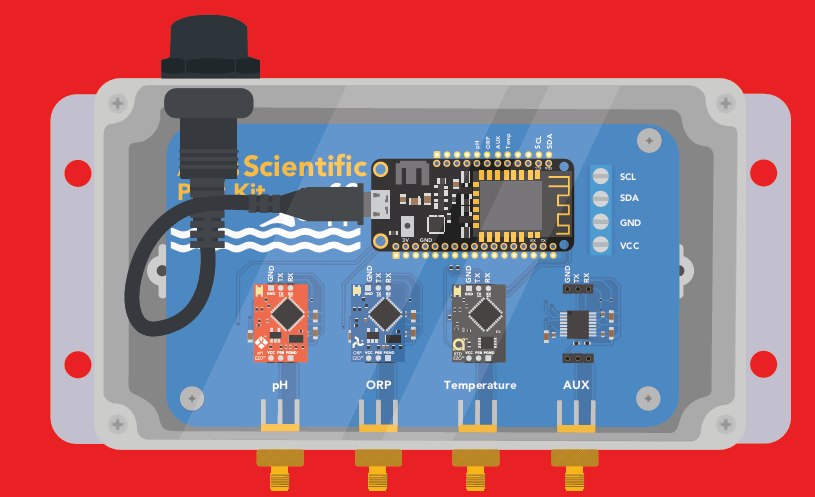
\includegraphics[scale=0.9]{imgss207.png}
	\caption{Esquema de la conexión en PCB. Imagen obtenida del manual \textit{Wi-Fi Pool Kit Setup Guide}}
	\label{fig:figura500_7}
\end{figure}

En la parte inferior de la \autoref{fig:figura500_7} se observan los conectores para las 4 sondas disponibles para lectura de datos, teniendo originalmente conexiones para las variables de temperatura, pH, y ORP; se cuenta 
en la conexión más a la derecha una cuarta opción adicional, pero el circuito de instrumentación debe ser elegido por el usuario según la variable que se requiera monitorear.

En la parte central se encuentran los espacios disponibles para las tarjetas PCB que ya montan circuitos para acondicionamiento de las señales eléctricas medidas por las sondas, para posteriormente transmitir al microcontrolador 
los valores de variables convertidos a su escala correspondiente. 

La \autoref{fig:figura500_8} muestra una imagen para el circuito de acondicionamiento del parámetro de temperatura.

\begin{figure}[h]
	\centering
	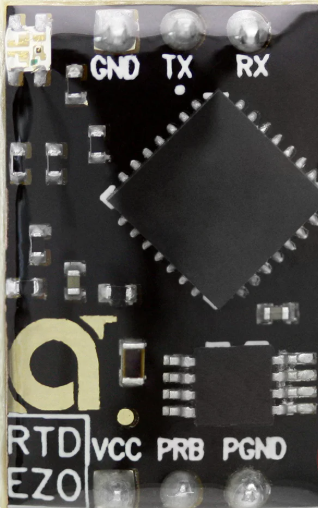
\includegraphics[scale=0.7]{imgss208.png}
	\caption{EZO RTD Temperature Circuit. Imagen obtenida del sitio \textit{https://atlas-scientific.com/}}
	\label{fig:figura500_8}
\end{figure}

Para este circuito el pin \textit{VCC} debe conectarse a una alimentación de 5V, el pin \textit{GND} requiere conexión a una tierra de referencia, y los pines \textit{TX} y \textit{RX} son las conexiones para transmisión y 
recepción de datos, respectivamente; estos pines llevan a los pines de comunicación correspondientes del ESP32. El protocolo de comunicación para esta tarjeta puede ser \textit{UART} o \textit{I2C}, sin embargo, para el ESP32 
se requiere exclusivamente usar \textit{I2C} como protocolo.

Otras características de esta tarjeta son las siguientes:

\begin{itemize}
    \item Resolución de 0.001 para las operaciones matemáticas de conversión de voltaje a salida de dato de temperatura.
    \item Capacidad para realizar máximo 1 lectura por segundo.
    \item Empleo del formato ASCII para la comunicación serial.
    \item Rango de voltaje de operación de 3.3V-5.5V.
\end{itemize}

La \autoref{fig:figura500_9} muestra una imagen para el circuito de acondicionamiento del parámetro de pH.

\clearpage

\begin{figure}[h]
	\centering
	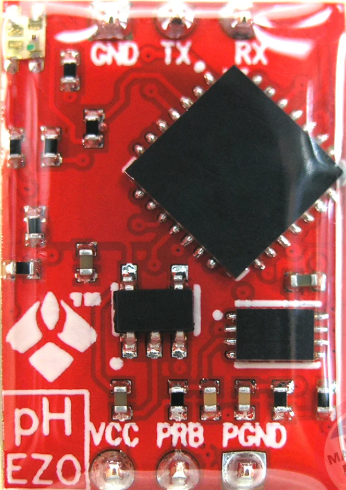
\includegraphics[scale=0.7]{imgss209.png}
	\caption{EZO pH Circuit. Imagen obtenida del sitio \textit{https://atlas-scientific.com/}}
	\label{fig:figura500_9}
\end{figure}

En esta tarjeta el pin \textit{VCC} debe conectarse a una alimentación de 5V, el pin \textit{GND} requiere conexión a una tierra de referencia, y los pines \textit{TX} y \textit{RX} son las conexiones para transmisión y 
recepción de datos, respectivamente; estos pines llevan a los pines de comunicación correspondientes del ESP32. El protocolo de comunicación para esta tarjeta puede ser \textit{UART} o \textit{I2C}, sin embargo, la comunicación 
serial con la tarjeta ESP32 requiere exclusivamente \textit{I2C} como protocolo.

Otras características de esta tarjeta son las siguientes:

\begin{itemize}
    \item Rango de medición en escala estándar de ph desde 0.001 hasta 14.000.
    \item Resolución de 0.001 para la conversión de voltaje a dato pH de salida.
    \item Tiempo de 800ms necesario para ejecutar una lectura.
    \item Capacidad de recibir señales de entrada de cualquier tipo de sonda especializada para el parámetro de pH.
    \item Capacidad para comunicación serial mediante \textit{I2C} o \textit{UART} como protocolos.
    \item Formato ASCII en la comunicación serial.
\end{itemize}

La \autoref{fig:figura500_10} muestra una imagen para el circuito de acondicionamiento del parámetro de ORP.

\clearpage

\begin{figure}[h]
	\centering
	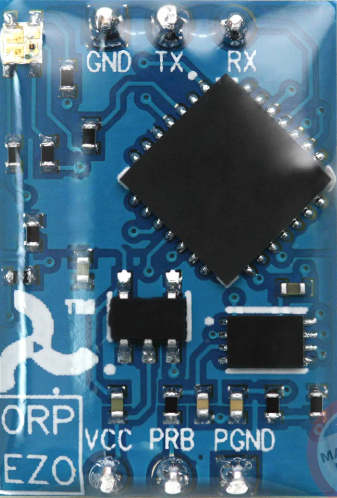
\includegraphics[scale=0.7]{imgss210.png}
	\caption{EZO ORP Circuit. Imagen obtenida del sitio \textit{https://atlas-scientific.com/}}
	\label{fig:figura500_10}
\end{figure}

Para esta tarjeta las conexiones de los pines son las mismas que las mencionadas para los casos anteriores, es decir, se requiere la alimentación de 5V, un punto de referencia a tierra y los pines de comunicación para la 
transmisión y recepción de datos con el dispositivo ESP32.

Las características principales para este circuito son las siguientes:

\begin{itemize}
    \item Rango de medición de voltaje de entrada desde -1.2V hasta 1.2V.
    \item Precisión de +/-1mV.
    \item Capacidad máxima de lectura de 1 dato por segundo.
    \item Compatibilidad para recibir señales de entrada de cualquier tipo de sonda para ORP.
    \item Comunicación serial UART o I2C mediante codificación ASCII.
    \item Su calibración se puede realizar para cualquier valor de ORP conocido.
\end{itemize}

La \autoref{fig:figura500_11} muestra una imagen para el circuito de acondicionamiento del parámetro de conductividad.

\clearpage

\begin{figure}[h]
	\centering
	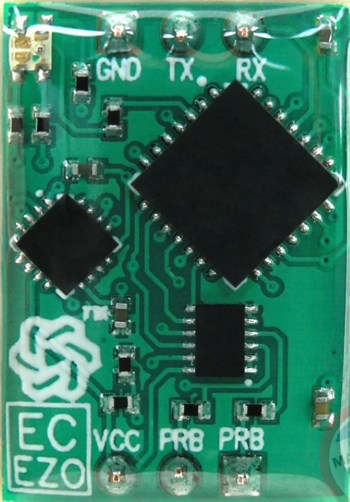
\includegraphics[scale=0.7]{imgss211.png}
	\caption{EZO Conductivity Circuit. Imagen obtenida del sitio \textit{https://atlas-scientific.com/}}
	\label{fig:figura500_11}
\end{figure}

Para este circuito se requiere alimentación de 5V en el pin \textit{VCC}, referencia de tierra para la conexión \textit{GND} y las conexiones para comunicación serial con el microcontrolador ESP32 en los pines \textit{TX} 
y \textit{RX}.

Las propiedades para esta tarjeta son las siguientes:

\begin{itemize}
    \item Capacidad para lecturas de los parámetros de conductividad, sólidos disueltos totales, salinidad y gravedad específica exclusivamente en agua de mar.
    \item Tiempo de 600ms requerido para ejecutar una lectura.
    \item Lecturas de 4 dígitos para valores de conductividad mayores o iguales a 10$\mu$S/cm.
    \item Lecturas de 3 dígitos para valores de conductividad igual o menores a 9.99$\mu$S/cm. 
\end{itemize}

Finalmente, la \autoref{fig:figura500_12} muestra el circuito para lecturas de la variable de oxígeno disuelto.

\clearpage

\begin{figure}[h]
	\centering
	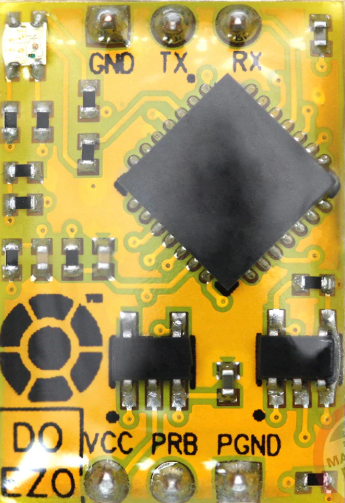
\includegraphics[scale=0.7]{imgss212.png}
	\caption{EZO Dissolved Oxygen Circuit. Imagen obtenida del sitio \textit{https://atlas-scientific.com/}}
	\label{fig:figura500_12}
\end{figure}

Los pines de conexión para esta placa requieren las mismas condiciones que los casos anteriores. Sus características principales son las siguientes:

\begin{itemize}
    \item Rango de lecturas de salida desde 0mg/L hasta 100mg/L. 
    \item Precisión de +/-0.05mg/L.
    \item Tiempo de 600ms requerido para la ejecución de cada lectura individual.
    \item Compatibilidad para lectura de voltajes de entrada exclusivamente de sondas de tipo galvánicas.
    \item Compensación para variaciones de temperatura, salinidad y presión atmosférica.
\end{itemize}

En lo referente a las conexiones de los circuitos de acondicionamiento de señal con el microcontrolador, en la \autoref{fig:figura500_13} se muestra un circuito esquemático de la conexión completa para el equipo Pool Kit.

\clearpage

\begin{figure}[h]
	\centering
	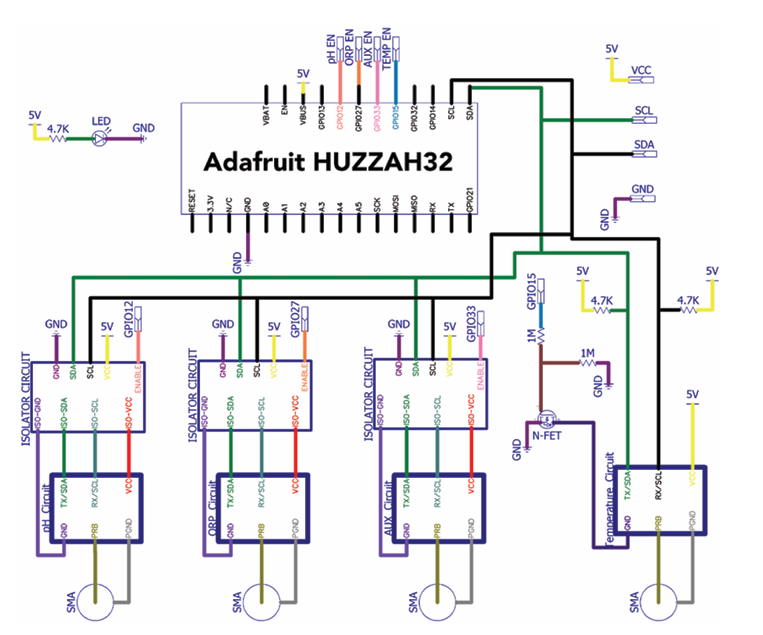
\includegraphics[scale=0.7]{imgss213.png}
	\caption{Diseño esquemático del PCB para el equipo Pool Kit. Imagen obtenida del manual \textit{Wi-Fi Pool Kit Setup Guide}}
	\label{fig:figura500_13}
\end{figure}

Para este diseño, los circuitos de ORP, pH y el AUX (circuito auxiliar) incluyen aislamiento electrico; el circuito de temperatura no contempla el aislamiento debido a que el elemento sensitivo en la sonda de temperatura 
no entra en contacto directo con el agua. Para esta implementación en específico la alimentación de todo el circuito se realiza a través del microcontrolador, así como también el punto de tierra de referencia se toma de 
la tarjeta del microcontrolador.

Es importante resaltar que esta implementación permite al usuario reemplazar los circuitos de acondicionamiento por otros para parámetros de calidad del agua diferentes. El único requisito es que los nuevos circuitos deben 
previamente estar diseñados o configurados para comunicación con I2C como protocolo, ya que en este caso el microcontrolador no esta adaptado para comunicación serial UART.

\section{Conclusiones}

En este capítulo se describen las posibilidades de generar equipo de medición para variables de calidad del agua al combinar sensores con el diseño de un sistema embebido compuesto de microcontrolador y tarjetas PCB con 
circuitos de instrumentación para acondicionamiento de las señales dadas por los sensores.

Es relevante cómo un número importante de parámetros de calidad del agua pueden ser monitoreados con este tipo de diseños, únicamente teniendo que cumplir los requerimientos de diseño específicos para cada circuito de 
instrumentación, atendiendo a las características individuales de cada señal eléctrica generada en los sensores para cada variable distinta.

\cleardoublepage
\chapter{Métodos Estadísticos Para Procesamiento de Datos}
\label{ch:Estadisticos}

\section{Conceptos Básicos}

La Estadística es una disciplina derivada de las Matemáticas que puede definirse de diferentes formas según el autor y su área de aplicación. En \cite{triola} se define la Estadística como una colección de métodos para planear 
experimentos, obtener datos, y después organizar, resumir, presentar, analizar, interpretar, y llegar a conclusiones basadas en los datos.    

En \cite{anderson} la Estadística se define como el arte y la ciencia de reunir datos, analizarlos e interpretarlos, lo cual permite mejorar la toma de decisiones en la aplicación específica donde estos métodos sean aplicables.

En las 2 definiciones anteriores hay un concepto que se repite, el de datos; ambas definiciones están construidas en torno a la palabra datos. Por lo tanto, desde aquí se puede apreciar que la Estadística se fundamenta y 
entrega resultados partiendo de datos o información que es buscada en el entorno de trabajo donde se desea aplicar la Estadística para la obtención de conclusiones.

En \cite{anderson} Datos se definen como hechos/informaciones y cifras numéricas que se recogen, analizan y resumen para su presentación e interpretación. 

\clearpage

\section{Tipos de Datos}

La \autoref{fig:figura600_1} muestra el diagrama de los tipos de datos usados en Estadística.

\begin{figure}[h]
	\centering
	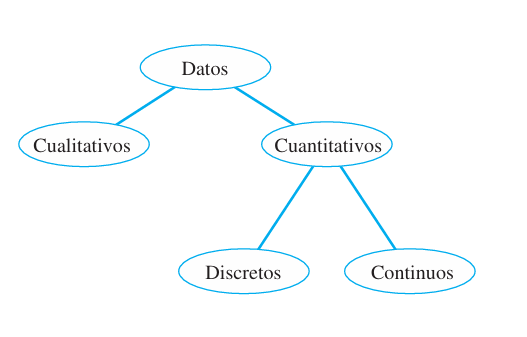
\includegraphics[scale=0.7]{imgss140.png}
	\caption{Tipos de datos}
	\label{fig:figura600_1}
\end{figure}

Los datos cualitativos son aquellos formados por etiquetas o nombres que permiten identificar un atributo de un objeto o persona \cite{anderson}. A los datos cualitativos también se les suele llamar datos categóricos o datos 
de atributo. Un ejemplo de este tipo de datos sería el color de una prenda de vestir, es decir, el dato \textit{color} podría tomar valores tales como azul, rojo, negro, verde, morado, entre otros.

Los datos cuantitativos son aquellos que consisten en números que representan conteos o mediciones \cite{triola}. Los datos cuantitativos pueden dividirse en 2 categorías, datos discretos y datos continuos.

Los datos discretos son aquellos que resultan cuando el número de posibles valores es un número finito, o bien, un número que puede contarse \cite{triola}. Un ejemplo de datos discretos sería la cantidad de personas presentes 
en un lugar específico.

Los datos continuos resultan de un número infinito de posibles valores que se pueden asociar a puntos de una escala continua, cubriendo un rango de valores sin huecos ni interrupciones \cite{triola}. Un ejemplo sería los 
valores de magnitud de la velocidad a la cual se desplaza un vehículo.

\section{Fuentes de Obtención de los Datos}

Se reconocen 2 métodos para la recolección de nuevos datos.

\begin{itemize}
    \item \textbf{Fuentes existentes}. Es posible que para una aplicación específica los datos requeridos ya existan. Por ejemplo, los sitios de internet gubernamentales contienen miles de bases de datos sobre diversas temáticas,
	y en su mayoría son de acceso libre con excepción de bases de datos que contengan datos confidenciales o información personal \cite{anderson}. 
    \item \textbf{Estudios estadísticos}. Es la metodología implementada cuando los datos no existen y deben obtenerse. Existen 2 tipos de estudios estadísticos, los experimentales y los observacionales. En la realización de un 
    estudio experimental primero se debe establecer cuál es la variable de interés, y después definir 1 o más variables de control, las cuales son modificadas para obtener información de cómo afectan a la variable de interés.
	Por otro lado, un estudio observacional consiste básicamente en la realización de una encuesta, por ejemplo, salir a realizar preguntar a un número definido de personas acerca del tema que se está estudiando \cite{anderson}. 
\end{itemize}

\clearpage

Adicionalmente, deben definirse 2 conceptos básicos relacionados con la recolección de datos en estadística.

\begin{itemize}
    \item \textbf{Variable}. Característica que cambia o varía con el tiempo para diferentes personas, objetos o entornos \cite{mendenhall}.
    \item \textbf{Unidad experimental}. Es el individuo, objeto o entorno en el que se mide una variable \cite{mendenhall}. 
    \item \textbf{Medición}. Dato obtenido para una variable \cite{mendenhall}.
    \item \textbf{Población}. Conjunto de mediciones de interés \cite{mendenhall}.
    \item \textbf{Muestra}. Subconjunto de mediciones obtenido de la Población \cite{mendenhall}.
\end{itemize}

\section{Estadística Descriptiva}

La estadística descriptiva consiste en la presentación o exposición de los datos recolectados, a través del uso de resúmenes, los cuales pueden ser tabulares, gráficos o numéricos \cite{anderson}.

Para nuestros propositos, los resúmenes de tipo numérico serán los de mayor utilidad acorde a las características del proyecto realizado.

\begin{itemize}
    \item \textbf{Media o Promedio}. El valor promedio de una variable proporciona una medida de localización central de los datos de una variable. Su cálculo tiene la forma (\ref{eq:ecuacion601}).
    \begin{equation}
	\mu=\frac{\sum_{i=0}^{N} {(x_i)}}{N}
	\label{eq:ecuacion601}
    \end{equation}

	Es decir, el valor promedio de un conjunto de datos es igual a la sumatoria de todos los datos, dividida entre el número de datos.

    \item \textbf{Mediana}. Para un conjunto de datos, la mediana es el valor de enmedio para dichos datos ordenados de menor a mayor, es decir, en forma ascendente \cite{anderson}. 
    
	Si el número de datos es impar, la mediana es el valor de enmedio. Si el número de datos es par, la mediana es el promedio de las 2 observaciones de enmedio \cite{anderson}. Si el número de datos es par, se puede usar 
	la ecuación (\ref{eq:ecuacion6058}) para obtener la mediana.
    
	\begin{equation}
	MED(X)=\frac{X(n/2) + X(1 + n/2)}{2}
	\label{eq:ecuacion6058}
    \end{equation}

	Es decir, la mediana de un conjunto de datos \textit{X} par se obtiene al sacar el promedio de los datos en las posiciones \textit{n/2} y \textit{1 + n/2} del arreglo de datos.

	\item \textbf{Moda}.La moda de un conjunto de datos es el valor que se repite con mayor frecuencia \cite{anderson}.
	\item \textbf{Rango}. El rango para un conjunto de datos es igual a la diferencia del valor mayor del conjunto y el valor menor \cite{anderson}.
	
	\begin{equation}
		Rango=Valor Mayor - Valor Menor
		\label{eq:ecuacion602}
	\end{equation}

	\item \textbf{Varianza}. La varianza de un conjunto de datos es una medida de su variabilidad, la cual se basa en la diferencia entre el valor de cada dato y el promedio de los datos; a dicha diferencia se le suele denominar \textit{desviación respecto a la media} \cite{anderson}.
	
	Si la varianza se calcula para los datos de una Población, se le conoce como \textit{varianza poblacional}, y se calcula de la forma (\ref{eq:ecuacion603})

	\begin{equation}
		\sigma^2=\frac{\Sigma (x_i - \mu)^2 }{N}
		\label{eq:ecuacion603}
	\end{equation}

	Si la varianza se calcula para datos que provienen de una muestra, se le dennomina \textit{varianza muestral} y se calcula de la forma (\ref{eq:ecuacion604})

	\begin{equation}
		s^2=\frac{\Sigma (x_i - \mu)^2 }{N-1}
		\label{eq:ecuacion604}
	\end{equation}

	A la varianza muestral se le considera el mejor estimador de la varianza poblacional para casos en donde no es posible el cálculo de la varianza poblacional debido principalmente a que no se conoce a toda la Población \cite{anderson}.

	\item \textbf{Desviación Estándar}. Se define como la raíz cuadrada positiva de la varianza \cite{anderson}. Al igual que para la varianza, para la desviación estándar existen la \textit{desviación estándar poblacional} (\ref{eq:ecuacion605})
	
	\begin{equation}
		\sigma=\sqrt{\sigma^2}
		\label{eq:ecuacion605}
	\end{equation}

	y la \textit{desviación estándar muestral} (\ref{eq:ecuacion606})

	\begin{equation}
		s=\sqrt{s^2}
		\label{eq:ecuacion606}
	\end{equation}

	De nuevo la desviación muestral es el mejor estimador de la desviación poblacional cuando su cálculo no es posible.

\end{itemize}

\subsection{Datos Atípicos}

Cuando se realiza la recolección de datos en una aplicación dada, y al analizarlos se detectan datos cuyos valores son mucho más grandes o mucho más pequeños que la mayoría de los datos recolectados, a estos valores extremos 
se les conoce como \textit{datos atípicos} u \textit{observaciones atípicas} \cite{anderson}.

Cuando se detectan este tipo de casos, es importante actuar con precaución acerca de cuál es la razón de tener datos atípicos. Es decir, puede que la causa sea que el investigador cometió un error al escribir el valor de 
un dato, algún error en la metodología o equipo de medición, pero también puede ser el caso de que el dato atípico realmente sí pertenezca al conjunto de datos, es decir, que no existe error en su recolección, por lo tanto, 
ese comportamiento inusual en los valores de los datos también deberá considerarse como parte del conjunto de datos \cite{anderson}.

\section{Coeficiente de Correlación Lineal de Pearson}

En estadística descriptiva al tener aplicaciones en las cuales en la mayoría de ellas se recolectan datos de una gran cantidad de variables, es conveniente realizar un análisis matemático acerca de si existen posibles 
relaciones entre algunas de estas variables. Pero, ¿qué tipo de relación entre ellas es útil buscar? Principalmente, el concepto de este análisis es tomar una variable como pivote, y ver qué ocurre con los datos de las 
demas variables cuando los datos de la variable pivote aumentan o decrecen en su magnitud de valor numérico. Por ejemplo, teniendo una variable pivote y una variable de prueba para análisis, se puede estudiar el comportamiento
de los datos de la variable de prueba cuando los datos de la variable pivote crecen o decrecen \cite{pinilla_pearson_2021}.

Primeramente, consideremos la \autoref{fig:figura600_2} 

\begin{figure}[h]
	\centering
	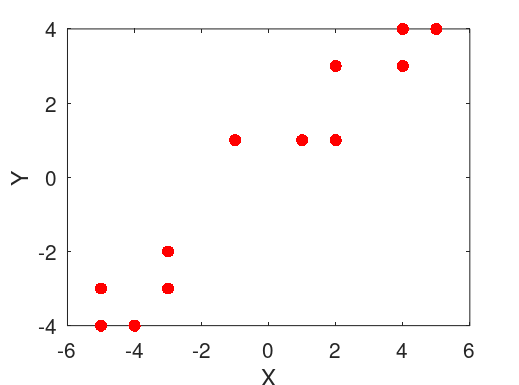
\includegraphics[scale=0.7]{imgss141.png}
	\caption{Relación lineal positiva entre 2 variables}
	\label{fig:figura600_2}
\end{figure}

En la \autoref{fig:figura600_2} podemos ver graficados los datos de 2 variables, "X vs Y". Se pueden establecer 2 conclusiones sobre los datos de dichas variables. La primera conclusión sería que de forma general el comportamiento 
entre dichas variables obedece a que cuando la variable X crece, la variable Y igualmente incrementa su valor. La segunda conclusión es sobre el hecho de que podríamos trazar una recta diagonal en la gráfica y dicha recta 
pareciera que sigue la tendencia marcada por los puntos. A partir de estas 2 conclusiones, podemos definir este comportamiento como una \textit{relación lineal positiva} entre las 2 variables contrastadas.

Ahora se considera la \autoref{fig:figura600_3}

\begin{figure}[h]
	\centering
	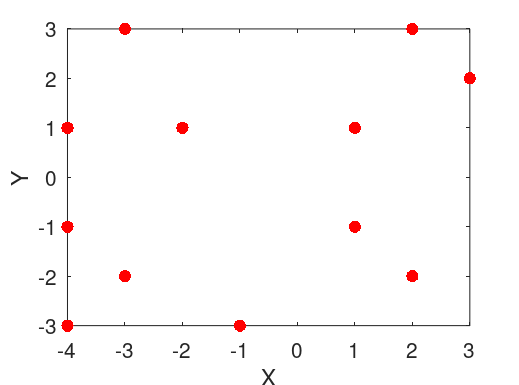
\includegraphics[scale=0.7]{imgss142.png}
	\caption{No existe relación lineal entre las variables}
	\label{fig:figura600_3}
\end{figure}

Igualmente, en la \autoref{fig:figura600_3} volvemos a tener un contraste de 2 variables "X vs Y". En este segundo caso, no se puede establecer que un incremento en la variable X esté correspondido con un incremento en 
la variable Y. De la misma forma, no se logra definir que una recta logre replicar el comportamiento de los datos marcados en la gráfica. Por lo tanto, para este segundo caso no existe ningún tipo de relación lineal.

Finalmente, consideremos la \autoref{fig:figura600_4}

\clearpage

\begin{figure}[h]
	\centering
	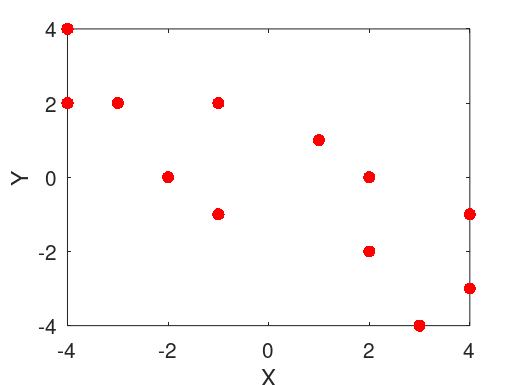
\includegraphics[scale=0.7]{imgss143.png}
	\caption{Relación lineal negativa entre 2 variables}
	\label{fig:figura600_4}
\end{figure}

Volvemos a tener un contraste entre variables "X vs Y". Para este tercer y último caso se puede observar una tendencia inversa entre las variables, es decir, cuando la variable X incrementa su valor, el comportamiento 
de la variable Y tiende a ser decreciente. Para este tipo de gráfica si trazamos de nuevo una recta en diagonal, ésta podra ayudarnos nuevamente a replicar la tendencia marcada por los datos, aunque en este tercer caso 
la recta tendrá una pendiente negativa. A este tipo de comportamiento entre 2 variables, se le denomina \textit{relación lineal negativa o inversa}.

Ahora que se sabe que pueden existir diferentes tipos de relación entre distintas variables, el objetivo en esta sección es cuantificar esa relación, es decir, obtener una medida numérica que pueda indicar el tipo de 
relación en caso de que exista, así como poder conocer la \textit{fuerza} de la relación entre 2 variables \cite{anderson}. Para esto se cuenta con la herramienta matemática del \textit{coeficiente de correlación de Pearson} (\ref{eq:ecuacion607})

\begin{equation}
	%r=\frac{\frac{\Sigma (x_i - \mu_x)(y_i - \mu_y) }{N}}{\sigma_x \sigma_y}
	r=\frac{1}{\sigma_x \sigma_y} \frac{\sum_{i=0}^{N} (x_i - \mu_x)(y_i - \mu_y)}{N}
	\label{eq:ecuacion607}
\end{equation}

Es decir, el cálculo de este indicador implica la sumatoria de los productos de las diferencias de los datos y sus promedios correspondientes, así como dividir estos resultados entre el producto de las desviaciones estándar
de cada una de las variables que se están comparando.

El rango de valores que puede tomar el coeficiente de Pearson abarca desde -1 hasta +1. Si el cálculo del coeficiente de Pearson entrega un resultado de +1, esto implica que los datos analizados se encuentran sobre una 
línea recta con pendiente positiva, conociéndose esto como una \textit{relación lineal positiva perfecta}. Por el contrario, si el cálculo del coeficiente entrega un resultado de -1, esto significa que los datos se encuentran 
sobre una línea recta con pendiente negativa, y a este caso se le conoce como \textit{relación lineal negativa perfecta} entre las 2 variables analizadas \cite{anderson}.

Si los datos de las variables comparadas muestran una relación lineal positiva, pero no es perfecta, esto implica que el valor del coeficiente sera menor a 1, indicando que no todos los puntos de la gráfica de los datos se 
encuentran sobre una línea recta. Entre más se desvién los puntos de una línea recta, menor sera el valor del coeficiente de correlación. Si el valor del coeficiente de correlación entrega un resultado de 0, significa que no 
existe una relación lineal entre las 2 variables analizadas; si el valor del coeficiente no es 0 pero cercano a dicho valor, significa que la relación lineal entre las 2 variables es \textit{débil} \cite{anderson}.

Finalmente, en este tema hay que dejar claro que el coeficiente de Pearson es un indicador de la medida de la relación lineal de 2 variables, mas no un indicador de causalidad. Es decir, si la correlación lineal entre 2 
parámetros es alta, esto no significa que los cambios que presente una de las variables, implique o genere cambios en la otra variable \cite{anderson} \cite{mendivelso_prueba_2022}.

\section{Conclusiones}

La estadística descriptiva tiene como objetivo tomar un conjunto de datos y realizar una caracterización de estos que permita conocer qué tipo de datos se tienen y el tipo de comportamiento que presentan. Para el trabajo 
desarrollado en esta tesis se ejecutan un cierto número de muestreos de agua en un proceso de potabilización, y dichas muestras serán analizadas para diferentes parámetros de calidad recolectando una gran cantidad de datos 
para cada una de las variables en estudio. Por lo tanto, la estadística descriptiva se convierte en la herramienta más útil para poder generar un panorama completo de las características que poseen los datos recolectados, 
lo que a su vez nos permite entender gran parte del comportamiento de la calidad del agua durante las diferentes etapas del proceso de potabilización.

Por otra parte, la herramienta del coeficiente de correlación lineal nos permite conocer si los diferentes parámetros de calidad del agua estudiados presentan entre ellos un patrón de comportamiento específico que nos permita 
establecer que dichas variables tienen ese patrón o tendencia debido a los cambios dados por el proceso de tratamiento. Además, el tener un nivel de correlación alto entre diferentes parámetros nos permite conocer el comportamiento 
de otras variables si se conoce el comportamiento de un parámetro específico. 

Todas las conclusiones y resultados que se pueden obtener de la aplicación de métodos estadísticos son la referencia principal que se puede seguir para la elección de las variables de calidad del agua que serán utilizadas 
como parámetros de entrenamiento en el modelo de red neuronal para clasificación de calidad del agua.

\cleardoublepage
\chapter{Proceso de Potabilización}
\label{ch:ProcesoOoapas}

El presente trabajo de tesis fue posible gracias al apoyo del OOAPAS (Organismo Operador de Agua Potable, Alcantarillado y Saneamiento de Morelia). Dicho organismo del gobierno municipal de la ciudad de Morelia nos permitió 
durante el año 2024 el acceso a una de sus plantas de potabilización, en la cual se nos permitió trabajar en su laboratorio de muestreo para realizar la recolección de los datos sobre las muestras obtenidas de las diferentes
etapas del proceso consideradas significativas para los propósitos establecidos en los objetivos y la metodología. En este capítulo se dará una descripción de las etapas que componen el proceso de potabilización llevado a 
cabo en esta planta, las cuales abarcan desde el agua que se recibe desde la presa captadora de agua que abastece a estas instalaciones hasta el producto final generado por el proceso, dicho producto es agua potable apta 
para su distribución.

En la \autoref{fig:figura947_1} se muestra un diagrama de las etapas que componen el proceso de potabilización estudiado.

La \autoref{fig:figura947_1} presenta el flujo del proceso de potabilización a través de sus diferentes etapas, además de indicar con una etiqueta en color rojo las fases del proceso que han sido previamente elegidas para 
la recolección de muestras.

\clearpage

\begin{figure}[h]
	\centering
	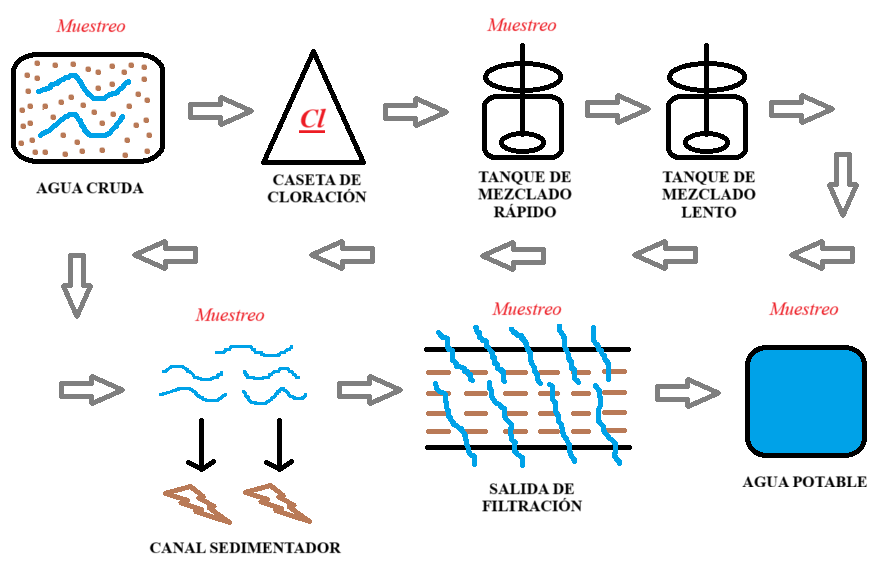
\includegraphics[scale=1]{imgss216.png}
	\caption{Etapas del proceso de potabilización}
	\label{fig:figura947_1}
\end{figure}

En la \autoref{fig:figura900_1}, se muestra el pozo que se tiene en la planta potabilizadora que permite acceder y poder extraer muestras del agua cruda que proviene 
directamente de la presa de Cointzio. La utilidad de poder extraer muestras de agua cruda radica en poder analizar sus parámetros fisicoquímicos y biológicos, y así 
poder conocer cuáles son las condiciones que se tienen en un momento específico en la presa en la cual se recolecta el agua, lo que permite determinar el nivel de 
contaminación presente en dicha presa. Sin embargo, el hecho de que pudiera llegar a la planta potabilizadora agua con niveles altos de contaminación, 
no necesariamenete indicaría que en la presa existiese por ejemplo un problema de que dicho cuerpo de agua tuviera en sí mismo problemas de contaminación. Podría ser 
incluso que los canales que transportan el agua de la presa a la planta requieran algún procedimiento de limpieza o retiro de basura que pudiera tener acumulada por el paso del tiempo.

Por ejemplo, durante los muestreos realizados en el mes de agosto de 2024, el agua recolectada de este pozo presentaba un nivel de contaminación muy alto debido a que, al ser época de lluvias, muchos contaminantes tanto 
artificiales como naturales son arrastrados por el agua de lluvia y logran filtrarse al agua que viaja desde la Presa de Cointzio hasta la planta de potabilización. Este sería un ejemplo de cómo factores externos pueden 
modificar de manera drástica la calidad del agua que se recibe en la planta, y por lo cual resulta imprescindible monitorear los diferentes parámetros en esta etapa del proceso para poder identificar si algún cambio es necesario 
en el proceso de potabilización para compensar los efectos sobre la calidad del agua cruda provocados por factores diversos.  

\clearpage

\begin{figure}[h]
	\centering
	\includegraphics[scale=0.05,angle=-90]{imgss12.jpg}
	\caption{Pozo de entrada de agua proveniente de la Presa de Cointzio}
	\label{fig:figura900_1}
\end{figure}

Una vez que el agua cruda ha ingresado a la planta, de las primeras acciones que se realizan es iniciar a inyectar agentes químicos desinfectantes, así como otras sustancias que ayudan a procesar los contaminantes presentes y 
posteriormente poder eliminarlos. Por otra parte, la razón de adicionar al agua sustancias desinfectantes desde el inicio del proceso es que se busca que dichas sustancias actuén durante todo el proceso y tengan una ventana de 
tiempo más amplia para poder cumplir su función.

En la \autoref{fig:figura900_2} se muestra el área donde se introduce al proceso el compuesto coagulante Sulfato de Aluminio. 

\begin{figure}[h]
	\centering
	\includegraphics[scale=0.05,angle=-90]{imgss13.jpg}
	\caption{Adición del coagulante Sulfato de Aluminio}
	\label{fig:figura900_2}
\end{figure}

\clearpage

Un proceso de coagulación permite la neutralización de los sólidos suspendidos en al agua que se encuentren cargados eléctricamente. Es decir, el reactivo coagulante 
agregado al agua presenta una carga eléctrica neta positiva, lo cual permite neutralizar la carga neta en el líquido al eliminar dicha carga negativa que viene en 
los sólidos suspendidos en el agua.

El hecho de poder eliminar la carga eléctrica neta presente permite que las partículas con el mismo tipo de carga no sufran constantemente fuerzas de repulsión entre ellas, logrando así posteriormente tener la posibilidad 
de agrupar todos estos residuos, lo cual facilita su separación al ya no tener dispersos a la mayor cantidad de dichos contaminantes.

En la \autoref{fig:figura900_3} se muestra la adición del compuesto floculante catiónico.

\begin{figure}[h]
	\centering
	\includegraphics[scale=0.05,angle=0]{imgss14.jpg}
	\caption{Adición del floculante catiónico}
	\label{fig:figura900_3}
\end{figure}

La función que realiza este reactivo es la de aglomerar partículas pequeñas o coloidales que se encuentran presentes en el agua, con el objetivo de lograr la formación 
de flóculos más grandes y densos, lo que posteriormente facilita su separación del agua en etapas posteriores del proceso.

Dado que en el agua cruda proveniente de la presa se tienen presentes una diversa cantidad de tipos de contaminantes, particularmente en el factor de sus dimensiones físicas, al tener partículas contaminantes de tamaño pequeño 
resulta conveniente poder agruparlas o juntarlas para facilitar su seperación en etapas posteriores del proceso, ya que si no se formaran flóculos con estos contaminantes probablemente sería necesario utilizar técnicas complejas 
de filtrado u otros métodos de separación. Por lo cual con la ayuda de agentes químicos se busca en esta etapa generar condiciones favorables para la eliminación de los residuos presentes en el liquído.

\clearpage

En la \autoref{fig:figura900_4} se muestra la caseta de cloración, en la cual se agrega dicho desinfectante.

\begin{figure}[h]
	\centering
	\includegraphics[scale=0.05,angle=0]{imgss15.jpg}
	\caption{Caseta de cloración}
	\label{fig:figura900_4}
\end{figure}

La adición de los reactivos desinfectantes es necesaria que se lleve a cabo en las etapas iniciales del proceso, de forma que se proporcione tiempo suficiente para que 
dichos reactivos logren eliminar la presencia bacteriológica antes de que el agua complete las etapas restantes de la potabilización y esté disponible para su distribución.

En esta etapa del proceso se ha comentado por parte del especialista del laboratorio de muestreo del OOAPAS que el nivel de calidad del agua presente en el agua cruda a la entrada de la planta es un factor determinante para 
poder tomar decisiones acerca de cómo debe realizarse la adición de agentes antibacteriológicos, particularmente en torno a la cantidad de sustancia a añadir. Por ejemplo, en época de lluvias cuando el agua cruda presenta un 
nivel de contaminación mayor, el proceso de desinfección debe mejorar para compensar esa mayor cantidad de material bacteriológico presente, lo cual se puede generar al elevar la cantidad de desinfectantes que se adicionan. Sin 
embargo, relacionado a esto también existe una restricción acerca de la cantidad de cloro que puede quedar presente en el agua potable una vez que ya se tiene el producto final del proceso. En esta parte nos tenemos que 
apoyar de la norma sanitaria correspondiente emitida por la Secretaria de Salud en conjunto con la Comisión Federal para la Protección contra Riesgos Sanitarios del Gobierno de México; la norma relativa para este caso específico 
es la Norma Oficial Mexicana NOM-127-SSA1. En ella se especifica que a la salida de un proceso de potabilización como el que se estudia en este proyecto el agua potable tiene un límite permisible para el cloro residual libre 
de 0.2mg/L a 1.5mg/L.
\clearpage
En la \autoref{fig:figura900_5} se muestran las siguientes etapas del proceso, los tanques de mezclado.

\begin{figure}[h]
	\centering
	\includegraphics[scale=0.05,angle=0]{imgss16.jpg}
	\caption{Tanques de mezclado}
	\label{fig:figura900_5}
\end{figure}

Aquí se tienen 2 tipos: tanque de mezclado rápido y tanque de mezclado lento.

El tanque de mezclado rápido se utiliza con el fin de disolver adecuadamente los contaminantes que se encuentren presentes en el agua, mientras que el tanque de mezclado lento ayuda en el proceso de formación de flóculos 
con los contaminantes sólidos para su posterior eliminación.

En esta parte del proceso, los tanques de mezclado rápido han sido una de las 5 etapas de donde se han tomado muestras para obtener datos de los parámetros fisicoquímicos analizados. En este caso se ha elegido particularmente 
ese tanque para poder tener una caracterización próxima entre las condiciones en el agua cruda y las condiciones en este tanque de mezclado, es decir, analizar etapas consecutivas para tener información de los efectos inmediatos 
en la calidad del agua justo después de la adición del coagulante, floculante y los agentes de desinfección.


En la \autoref{fig:figura900_6} se muestra el canal de sedimentación, la etapa del proceso siguiente a los 2 tipos de tanque de mezclado.
\clearpage
\begin{figure}[h]
	\centering
	\includegraphics[scale=0.3,angle=0]{imgss17.jpg}
	\caption{Canal de sedimentación}
	\label{fig:figura900_6}
\end{figure}

Aquí se busca que toda la basura y contaminantes sólidos, una vez que ha terminado el proceso de floculación, puedan sedimentarse, es decir, que todo ese material sólido transportado por la corriente de agua, se pueda hundir 
o depositar en el fondo por efectos de gravedad. En esta etapa de separación de contaminantes se logra eliminar un porcentaje muy importante de los residuos presentes en el agua, ya que si se hace la compartiva de una muestra
correspondiente al canal de sedimentación contra una muestra de los tanques de mezclado, prácticamente todos los residuos de gran tamaño han desaparecido en la muestra correspondiente al canal, cuando la muestra de cualquiera
de los tanques de mezclado tiene presente una gran cantidad de flóculos formados por los contaminantes. Además el color del agua en cualquiera de los tanques es tonalidades cafés, y en el agua que se puede recolectar del 
canal de sedimentación ya existe una condición incolora.

\clearpage

Posteriormente, la etapa siguiente son los filtros, los cuales se muestran en la \autoref{fig:figura900_7}.

\begin{figure}[h]
	\centering
	\includegraphics[scale=0.05,angle=0]{imgss18.jpg}
	\caption{Filtros}
	\label{fig:figura900_7}
\end{figure}

En la planta de potabilización se ha explicado que el tipo de filtrado realizado en este caso particular es el método de filtrado por gravedad, en el cual el líquido atraviesa un conjunto de capas, las cuales retienen las 
particulas sólidas que aún estén presentes. Estos filtros son la última etapa del proceso donde se ejecuta algún procedimiento físico para eliminación de contaminantes; la continuación del proceso después de esta última 
etapa de filtrado es un tanque de almacenamiento que se encuentra por debajo del suelo, en el cual el agua se almacena temporalmente una vez que ha terminado el filtrado.  

En la \autoref{fig:figura900_8} se muestran los canales que transportan el agua potabilizada lista para distribución.

\clearpage

\begin{figure}[h]
	\centering
	\includegraphics[scale=0.05,angle=0]{imgss19.jpg}
	\caption{Salida del proceso, agua potable}
	\label{fig:figura900_8}
\end{figure}

Es por estos canales por donde el agua pasa al sistema de distribución después de haber estado en el tanque de almacenamiento una vez que terminó el filtrado. 

Por lo tanto, de forma general el proceso consiste primeramente en la adición de los reactivos para coagulación y floculación, de forma que en los tanques de mezclado y el canal de 
sedimentación pueda quedar atrapada la mayor parte de los componentes sólidos. Además, inicalmente también se han agregado los desinfectantes para que estos actuen durante el proceso
y al final del mismo, el proceso de desinfección tuviese el tiempo suficiente para llevarse a cabo adecuadamente. Finalmente, antes de la salida del proceso donde ya se tiene agua potable para 
distribución, también se realiza la etapa de filtrado donde se retienen las partículas más pequeñas que no pudieron ser eliminadas por sedimentación.

Ahora, en lo referente al seguimiento preventivo que realiza el OOAPAS para vigilar el estado del conjunto de parámetros de calidad del agua que ellos manejan, se sigue un proceso diario de recolección de muestras en diferentes 
puntos del proceso. Esta toma de muestras es realizada por las mañanas y el líquido recolectado es llevado a los laboratorios de la planta para realizar pruebas de bacteriología, pruebas de propiedades químicas y propiedades 
físicas. Con estos ensayos es que se puede verificar el cumplimiento de la normativa que regula este tipo de proceso de tratamiento, que se tiene específicamente la regulación NOM-127-SSA1-2021 de agua para uso y consumo 
humano y sus límites permisibles de calidad.

\section{Conclusiones}

Este proyecto tiene como uno de sus propósitos el realizar mediciones para diversas variables de calidad del agua en el proceso de potabilización del OOAPAS. Es importante que previamente a comenzar la toma de muestras, 
se tenga el entendimiento acerca las partes que componen el proceso que se va a estudiar. En este capítulo se presenta la descripción etapa por etapa del proceso a caracterizar, haciendo uso de imágenes y explicando la función 
o propósito específico de cada fase del proceso, lo cual ayuda a relacionar las diferentes etapas al comprender los cambios que se van produciendo conforme fluye el líquido por el proceso, logrando identificar la dependencia 
que existe entre dichas etapas.

\cleardoublepage
%!TeX root=../thesisStructure.tex
% Chapter 2
\chapter{Desarrollo y Resultados} % Chapter title
\label{ch:MarcoTeorico} 

\section{Recolección de muestras del proceso de potabilización}

Para poder iniciar con la tarea de recolección de muestras en la planta de potabilización, primero era necesario conocer los puntos en los cuales las muestras serían tomadas. Por lo tanto, tomando en cuenta las recomendaciones 
dadas por los especialistas de la planta de tratamiento y los resultados de trabajos previos realizados en esa instalación, se determinó que los puntos de agua cruda, tanque de mezclado rápido, canal sedimentador, salida 
de los filtros y la salida de agua potable serían las fases consideradas para muestreo.

Referente a la elección de las 5 etapas para muestreo, es evidente que el análisis de la entrada del proceso, agua cruda, es fundamental para tener la referencia inicial de los parámetros de calidad para líquido con nulo 
tratamiento, lo cual nos permite conocer las condiciones iniciales y así observar cómo los parámetros cambian gradualmente durante el proceso. Posteriormente, se eligen 3 etapas intermedias del proceso que no sean subsecuentes,
lo cual es importante para que los cambios en la calidad del agua sea de mayor magnitud. Además, la importancia de tener registro completo de los cambios en la calidad del agua entre la entrada y salida del proceso. Finalmente, 
la base de datos generada debe tener registro de la calidad en el producto final del proceso, lo cual permite completar la caracterización de las variables de calidad que se estarán analizando.

La obtención de muestras de agua se ha realizado directamente en la planta de potabilización en las etapas específicas del proceso determinadas previamente. Esta recolección de muestras de líquido desde la planta se realizó 
a lo largo del año 2024, dividiendo temporalmente los muestreos para las diferentes estaciones del año, con el fin de tener evidencia para los diferentes tipos de clima que se presentan.

La medición de las muestras recolectadas inicialmente se llevó a cabo en los laboratorios del ITM después de que se realizaba el traslado de las muestras desde la planta. Posteriormente, las mediciones se comenzaron a llevar 
a cabo en el laboratorio de muestreo de la planta de potabilización. Para la medición de los diferentes parámetros considerados durante el proyecto, se estuvo haciendo uso del equipo de medición Pool Kit junto con los diferentes 
sensores del mismo fabricante Atlas Scientific para cada variable individual. Adicionalmente, en el laboratorio de muestreo del OOAPAS también se nos permitió uso de su equipo de medición para realizar mediciones puntuales 
en casos en los cuales no era posible el uso de nuestro equipo.

La primera caracterización del proceso de potabilización se realizó en enero de 2024. Esta primera caracterización fue llevada a cabo con muestras recolectadas previamente, de las cuales 
se obtuvieron pequeñas cantidades correspondientes a las etapas específicas. En esta caracterización los parámetros medidos fueron ORP, temperatura, pH y conductividad; para cada una de las 5 muestras 
se realizaron 3 mediciones, cada una de ellas de una duración aproximada de entre 15 y 20 minutos. Es decir, primeramente se introducen los sensores a la muestra de agua durante el tiempo determinado, posteriormente se 
sacan para enjuagarlos y limpiarlos con agua destilada, para posteriormente volver a introducirlos durante el tiempo establecido. 

Al mismo tiempo que se realiza la medición de las muestras, los datos registrados por los sensores se almacenan y etiquetan en archivos de tipo CSV. Particularmente para este primer experimento, los datos recolectados no han 
podido ser considerados confiables debido a que las muestras medidas tenían varíos días de haberse recolectado de la planta, lo que genera su deterioro y la pérdida de sus propiedades y características que se 
busca analizar. Por lo cual es importante que las mediciones se realicen sin dejar pasar mucho tiempo una vez que las muestras son extraídas en la planta.


%\tikzstyle{startstop} = [rectangle, rounded corners, 
						%minimum width=3cm, 
						%minimum height=1cm,
						%text centered, 
						%draw=black, 
						%fill=red!30]

%\tikzstyle{io} = [trapezium, 
				  %trapezium stretches=true, % A later addition
				  %trapezium left angle=70, 
				  %trapezium right angle=110, 
				  %minimum width=3cm, 
				  %minimum height=1cm, text centered, 
				  %draw=black, fill=blue!30]

%\tikzstyle{process} = [rectangle, 
					   %minimum width=3cm, 
					   %minimum height=1cm, 
					   %text centered, 
					   %text width=3cm, 
					   %draw=black, 
					   %fill=orange!30]

%\tikzstyle{decision} = [diamond, 
						%minimum width=3cm, 
						%minimum height=1cm, 
						%text centered, 
						%draw=black, 
						%fill=green!30]
%\tikzstyle{arrow} = [thick,->,>=stealth]

%\begin{center}
%\begin{tikzpicture}[node distance=2cm]

	%\centering

	%\node (start) [startstop] {\textbf{AGUA CRUDA}};
	%\node (in1) [process, below of=start,yshift=-0.2cm] {COAGULACIÓN Y FLOCULACIÓN};
	%\node (pro1) [process, below of=in1,yshift=-0.2cm] {CASETA DE CLORACIÓN};
	%\node (dec1) [startstop, below of=pro1, yshift=-0.2cm] {\textbf{TANQUE DE MEZCLA RÁPIDA}};
	%\node (indz100) [process, below of=dec1, yshift=-0.2cm] {TANQUE DE MEZCLA LENTA};
    %\node (indz101) [startstop, below of=indz100, yshift=-0.2cm] {\textbf{CANAL SEDIMENTADOR}};
	%\node (indz102) [process, below of=indz101, yshift=-0.2cm] {FILTROS};
	%\node (indz103) [startstop, below of=indz102, yshift=-0.2cm] {\textbf{SALIDA DE FILTROS}};
	%\node (indz104) [process, below of=indz103, yshift=-0.2cm] {TANQUE DE ALMACENAMIENTO};
	%\node (indz105) [startstop, below of=indz104, yshift=-0.2cm] {\textbf{AGUA POTABLE}};	
														   
%\end{tikzpicture}
%\end{center}

Finalmente, en la primera caracterización del proceso se ha establecido la metodología de medición que se llevará a cabo para los siguientes muestreos. Básicamente esta parte está relacionada con los cuidados que se debe tener 
en el manejo de las muestras de agua y del equipo de medición. En cuanto al manejo de las muestras de agua, la parte fundamental es la limpieza necesaria en los frascos donde se recolecta el líquido para evitar contaminación 
de las muestras. En lo referente al equipo de medición, el cuidado especial igualmente es sobre la limpieza y enjuague de los sensores al cambiar entre muestras de diferentes etapas para evitar muestras contaminadas. 

En la segunda caracterización del proceso de potabilización, llevada a cabo en el mes de febrero, se miden las variables de temperatura, pH, ORP y conductividad. En este segundo experimento las mediciones fueron efectuadas 
en un periodo de tiempo de 4 días, y para este segundo muestreo dicho factor ha sido por el cual se nos ha hecho la recomendación de efectuar las mediciones el mismo día que las muestras son extraídas, y en caso de tardar 
más de 1 día, es recomendable refrigerar las muestras para evitar su deterioro.

La tercera caracterización se efectuó el día 6 de marzo de 2024 y los parámetros medidos fueron temperatura, pH, ORP y conductividad. La recolección de las muestras 
se realizó 1 día antes, el 5 de marzo por la tarde, y la totalidad de las mediciones se efectuaron el dia siguiente, teniendo en esta ocasión una duración aproximada de 40 minutos 
de monitoreo para cada 1 de las 5 muestras recolectadas. En esta tercera caracterización el cambio importante efectuado durante el monitoreo de las muestras fue el orden en que se hacían las mediciones. A partir de este 
experimento y para los siguientes se definió que las mediciones se harían en el orden inverso al avance dado por el proceso, es decir, la primera medición se hace sobre la muestra de agua potable, en segundo 
lugar la muestra de salida de filtración, en tercer lugar la muestra de canal sedimentador, posteriormente la muestra de tanque de mezclado rápido, y por último la muestra de agua cruda. 

La conclusión para la tercera caracterización ha sido sobre el descarte de las variables de temperatura, pH y conductividad para modelos de clasificación. Esta determinación se ha hecho tomando como referencia resultados 
estadísticos que se presentan en la sección siguiente de este capítulo.

La cuarta caracterización fue llevada a cabo los días 12 y 13 de marzo de 2024, siendo las etapas de agua potable y salida de filtración caracterizadas el primer día por la tarde y las 3 etapas anteriores medidas por la 
mañana del 13 de marzo; para este experimento se dejaron de considerar los parámetros de pH y conductividad eléctrica, y se agregó al equipo Pool Kit un sensor de oxígeno disuelto, además de que en el laboratorio de muestreo 
del OOAPAS nos proporcionaron los datos puntuales para el parámetro de cloro residual. 

Los resultados finales de la cuarta caracterización entregaron los comportamientos esperados tanto para los parámetros que ya se tenían como para los parámetros incluidos en este experimento. Principalmente en el caso de 
cloro residual, en las primeras 3 etapas, agua cruda, tanque de mezcla rápida y canal sedimentador, no hubo presencia. Fue hasta las 2 útimas etapas, salida de filtros y agua potable, que ya pudo detectar 
la presencia de remanentes del agente desinfectante.

La quinta caracterización se llevó a cabo los días 23 y 24 de abril, teniendo que las etapas de agua potable y salida de filtración se midieron la tarde del primer día, y las etapas de agua cruda, tanque de mezclado rápido 
y canal sedimentador se caracterizaron el segundo día por la mañana. Las variables medidas en este experimento fueron temperatura, oxígeno disuelto y ORP; el parámetro de cloro residual no pudo obtenerse ya que 
en el laboratorio de calidad del agua en el OOAPAS no hubo disponibilidad de que se nos proporcionara esa información. Adicionalmente, en este quinto experimento el tiempo de medición fue aproximadamente de 40 minutos para 
cada 1 de las 5 muestras.

La quinta caracterización entregó resultados importantes sobre la variable de oxígeno disuelto que derivaron en decisiones sobre un cambio significativo en la metodología de trabajo. Al final de este quinto experimento, 
los rangos de valores para oxígeno disuelto en las distintas etapas no presentaron una tendencia que permitiera diferenciar claramente las etapas del proceso con el uso de este parámetro. Por lo tanto, en este momento se decidió 
trasladar el equipo de instrumentación al laboratorio de muestreo del OOAPAS, ya que hasta este punto los monitoreos se hacían después de que las muestras de agua eran extraídas 
de la planta y posteriormente trasladadas al laboratorio de posgrado del Tecnológico. Esto permite evitar cambios no deseados en los parámetros analizados, ya que dichos parámetros son afectados por los cambios de 
temperatura.

Para la sexta caracterización, la fecha de realización corresponde al día 02 de julio de 2024. Para las muestras recolectadas ahora las mediciones se han llevado a cabo en el laboratorio de muestreo 
en la planta de potabilización. Referente a las diferencias que se pueden observar en los datos recolectados ahora que la caracterización
se realiza inmediatamente después de la recolección de la muestras, por ejemplo, está el caso del oxígeno disuelto. Para este parámetro se tiene el siguiente problema. Cuando en un recipiente o frasco como los que se usan 
en esta investigación para la recolección de las muestras, estos frascos contienen el agua de una fase específica y al mismo tiempo el líquido contenido conserva el oxígeno disuelto 
que ha ido atrapando en su recorrido. Sin embargo, que el agua contenida en los frascos pueda retener el oxígeno disuelto en ella, depende de la solubilidad de dicho gas, la cual a su vez depende de las condiciones de temperatura 
y presión a las que se encuentra la muestra. 

Es decir, se puede mantener los frascos cerrados y conservar el mismo valor de presión en la muestra, pero en el traslado de las muestras de la planta de potabilización al laboratorio 
del ITM se genera un aumento de temperatura. Es aquí donde existe un problema con el oxígeno disuelto; un aumento de temperatura en una muestra contenida en un 
frasco en esas condiciones, generará un descenso en la solubilidad del gas oxígeno existente en el agua.
Por lo tanto, si la caracterización de las muestras se hace una vez que se han llevado al laboratorio de posgrado, los valores medidos para oxígeno disuelto serán menores en comparación con las condiciones reales, ya que 
el aumento de temperatura genera descenso en la solubilidad del oxígeno en el agua, lo cual genera una pérdida de dicho gas una vez que los frascos son abiertos. 

Para esta sexta caracterización, se realizaron 3 muestreos el mismo día; el primero, a las 9 de la mañana; el segundo, a la 1 de la tarde; el tercero, a las 5 de la tarde. Para esta fecha en la que se realiza esta sexta 
caracterización, ya la ciudad de Morelia se encuentra en época de lluvias, por lo cual se generan escurrimientos los cuales contienen una gran cantidad de contaminantes, los cuales se mezclan con el agua que llega a la planta
para su tratamiento; entre los contaminantes que se pueden agregar se encuentran por ejemplo todo lo que se arrastra por el suelo, tanto subterráneo como lo que se encuentra sobre las carreteras, tales como aceite de automóviles,
químicos fertilizantes o la simple mezcla de lodo que escurre de las montañas y se incorpora al agua que llega a la planta de potabilización. Es importante tener en cuenta que la época de lluvias termina aproximadamente a 
mediados de octubre, por lo cual las caracterizaciones realizadas a partir de esta fecha y hasta el final de la época de lluvias, será importante tener ciertas consideraciones sobre efectos no deseados en los valores para 
los datos recolectados. 

En la \autoref{tab:table20000_1} se muestran los coeficientes de correlación para los datos del sexto experimento.

\begin{table}[h]
	\begin{center}
		\begin{tabular}{| c | c | c | c | c | c |}
			\hline
			\multicolumn{6}{ |c| }{Matriz de correlación Pearson} \\ \hline
			 & Temperatura & DO & ORP & Conductividad & Cloro Residual \\ \hline
			 Temperatura & 1 & 0.7564 & 0.7279 & 0.1051 & 0.4286 \\
			 DO & 0.7564 & 1 & 0.823 & -0.0069 & 0.6775 \\
			 ORP & 0.7279 & 0.823 & 1 & -0.1727 & 0.6874 \\
			 Conductividad & 0.1051 & -0.0069 & -0.1727 & 1 & -0.2738 \\ 
			 Cloro Residual & 0.4286 & 0.6775 & 0.6874 & -0.2738 & 1 \\ \hline
			 \multicolumn{6}{ |c| }{Matriz de correlación Spearman} \\ \hline
			 & Temperatura & DO & ORP & Conductividad & Cloro Residual \\ \hline
			 Temperatura & 1 & 0.7268 & 0.7567 & 0.3267 & 0.4093 \\
			 DO & 0.7268 & 1 & 0.8167 & 0.0349 & 0.7184 \\
			 ORP & 0.7567 & 0.8167 & 1 & 0.0041 & 0.7093 \\
			 Conductividad & 0.3267 & 0.0349 & 0.0041 & 1 & -0.1939 \\
			 Cloro Residual & 0.4093 & 0.7184 & 0.7093 & -0.1939 & 1 \\ \hline
		\end{tabular}
		\caption{Coeficientes de correlación para la sexta caracterización}
		\label{tab:table20000_1}
	\end{center}
\end{table}

En la \autoref{tab:table20000_1} se observa que los coeficientes de correlación son altos para los parámetros de ORP, cloro residual y oxígeno disuelto. Esto implica que los cambios en la metodología en la toma de mediciones 
ha generado resultados más cercanos a lo establecido en la teoría.

La séptima caracterización fue realizada el día 04 de julio de 2024 y los parámetros significativos medidos fueron oxígeno disuelto, ORP y cloro residual. Al igual que para la sexta caracterización, nuevamente 
se hizó 3 veces la recolección de muestras en horarios establecidos; 9 de la mañana, primera recolección; 1 de la tarde, segunda recolección; 5 de la tarde, la tercera muestra. Igualmente, el análisis de las muestras se llevó 
a cabo en el laboratorio de muestreo de la planta de potabilización. 

La octava caracterización se llevó a cabo el día 09 de julio de 2024 y los parámetros significativos monitoreados fueron de nuevo ORP, cloro residual y oxíegno disuelto. Para este octavo experimento, se pidió 
un cambio en la metodología específicamente para esta caracterización, ya que se buscaba hacer un análisis acerca de si para este proceso de potabilización los parámetros  que se están estudiando tienen 
variaciones rápidas a lo largo del día. Lo que se pidió fue realizar recolección de muestras del proceso cada 2 horas durante el transcurso de este día, y medir las variables para poder determinar 
si existiesen variaciones significativas de los parámetros en el rango de tiempo de 1 día. En esta ocasión sólo se recolectaron muestras de 2 etapas del proceso, tanque de mezcla rápida y agua potable, debido a que no se contaba 
con el tiempo necesario para medir las 5 etapas en un rango de tiempo de 2 horas. Los horarios de recolección de muestras se plantearon que 
fuesen a las 10 de la mañana, 12 de la tarde, 2 de la tarde, 4 de la tarde y 6 de la tarde, sin embargo, la última recolección no se pudo ejecutar debido a las condiciones de lluvia.

Para el caso de la variable de ORP en la etapa de tanque de mezcla rápida, se muestran los resultados de los datos medidos en la \autoref{fig:figura1000_4}, \autoref{fig:figura1000_5}, \autoref{fig:figura1000_6} y \autoref{fig:figura1000_7}.
En los ejes horizontales se tiene el número de muestras y la magnitud de la variable se encuentra en el eje vertical de las gráficas.

\clearpage

\begin{figure}[h]
	\centering
	\includegraphics[scale=0.7]{imgss157.png}
	\caption{ORP en tanque de mezclado a las 10 de la mañana.}
	\label{fig:figura1000_4}
\end{figure}

\begin{figure}[h]
	\centering
	\includegraphics[scale=0.7]{imgss158.png}
	\caption{ORP en tanque de mezclado a las 12 de la tarde.}
	\label{fig:figura1000_5}
\end{figure}

\clearpage

\begin{figure}[h]
	\centering
	\includegraphics[scale=0.7]{imgss159.png}
	\caption{ORP en tanque de mezclado a las 2 de la tarde.}
	\label{fig:figura1000_6}
\end{figure}

\begin{figure}[h]
	\centering
	\includegraphics[scale=0.7]{imgss160.png}
	\caption{ORP en tanque de mezclado a las 4 de la tarde.}
	\label{fig:figura1000_7}
\end{figure}

Para la etapa de agua potable, se muestran las siguientes mediciones en los diferentes horarios en la \autoref{fig:figura1000_8}, \autoref{fig:figura1000_9}, \autoref{fig:figura1000_10} y \autoref{fig:figura1000_11}. 
En los ejes horizontales se tiene el número de muestras y la magnitud de la variable se encuentra en el eje vertical de las gráficas.

\clearpage

\begin{figure}[h]
	\centering
	\includegraphics[scale=0.7]{imgss161.png}
	\caption{ORP en agua potable a las 10 de la mañana.}
	\label{fig:figura1000_8}
\end{figure}

\begin{figure}[h]
	\centering
	\includegraphics[scale=0.7]{imgss162.png}
	\caption{ORP en agua potable a las 12 de la tarde.}
	\label{fig:figura1000_9}
\end{figure}

\clearpage

\begin{figure}[h]
	\centering
	\includegraphics[scale=0.7]{imgss163.png}
	\caption{ORP en agua potable a las 2 de la tarde.}
	\label{fig:figura1000_10}
\end{figure}

\begin{figure}[h]
	\centering
	\includegraphics[scale=0.7]{imgss164.png}
	\caption{ORP en agua potable a las 4 de la tarde.}
	\label{fig:figura1000_11}
\end{figure}

En el caso de los parámetros de cloro residual y oxígeno disuelto no se registraron cambios a lo largo de los diferentes horarios muestreados. 

La novena y décima caracterizaciones fueron llevadas a cabo los días 06 y 08 de agosto respectivamente. En estos 2 experimentos se volvió a tomar muestras de las 5 etapas predeterminadas. Para el noveno y décimo experimento se solicitó que las mediciones fuesen modificadas 
para esta ocasión en específico. La petición en estas 2 caracterizaciones fue que la medición en cada una de las 5 muestras fuese de 35 minutos sin interrupciones. El objetivo de este cambio era poder observar el comportamiento de la estabilización en las mediciones para 
un periodo de tiempo más extenso, ya que los sensores utilizados, al principio de la medición, pueden presentar variaciones, pero con el paso de los minutos tanto el sensor como la muestra de agua se estabilizan, y ese fenómeno 
en específico es el que se buscaba registrar.

Sin embargo, las mediciones para la novena y décima caracterización fueron afectadas debido al nivel de contaminación que presentaba el agua cruda debido a todos los residuos generados por 
las lluvias. En estos casos, el agua cruda presentaba un color completamente café, además de tener una consistencia lodosa, respecto a lo cual en el laboratorio de muestreo se nos comentó que esas condiciones 
son principalmente ocasionadas por la filtración de arcilla. Estas condiciones generaron valores en las mediciones fuera de lo esperado, lo cual nos permite conocer que las lluvias son un factor que generan cambios que 
afectaran las mediciones con el equipo específico que hemos utilizado.

Para la décimo primera caracterización su fecha de realización fue el día 12 de noviembre de 2024. En estas fechas el agua cruda que llegaba a la planta ya no presentaba el alto nivel de contaminación que se encontró en 
las mediciones llevadas a cabo en el mes de agosto, ahora las condiciones del agua cruda eran de nuevo similares a las que se podían observar entre los meses de enero y julio. Para este experimento las variables medidas 
fueron ORP, cloro residual y oxígeno disuelto. 

En la \autoref{tab:table25000_1} se muestran los coeficientes de correlación para los datos del onceavo experimento.

\begin{table}[h]
	\begin{center}
		\begin{tabular}{| c | c | c | c |}
			\hline
			\multicolumn{4}{ |c| }{Matriz de correlación Pearson} \\ \hline
			 & DO & ORP & Cloro Residual \\ \hline
			 DO & 1 & 0.8857 & 0.9071 \\
			 ORP & 0.8857 & 1 & 0.984 \\
			 Cloro Residual & 0.9071 & 0.984 & 1 \\ \hline
		\end{tabular}
		\caption{Coeficientes de correlación para la onceava caracterización}
		\label{tab:table25000_1}
	\end{center}
\end{table}

Se observa que los coeficientes entre los parámetros significativos tienen magnitud cercana a 1, lo cual es la tendencia deseada. Este tipo de comportamiento era imposible de obtener para las mediciones del mes de agosto 
cuando las condiciones de contaminación generaban mediciones fuera de rango para las variables medidas.

La doceava caracterización se realizó el día 14 de noviembre de 2024, en la cual los parámetros medidos fueron ORP, cloro residual y oxígeno disuelto. En esta ocasión fueron realizados 3 recolecciones 
de muestras a diferentes horarios, 9 de la mañana, 1 de la tarde y 5 de la tarde, y las 3 recolecciones fueron sobre las 5 etapas del proceso predeterminadas.

Finalmente, la última caracterización fue realizada el día 19 de noviembre de 2024, en la cual se analizaron los parámetros de ORP, cloro residual y oxígeno disuelto para las 5 etapas predeterminadas.
Se realizaron 2 recolecciones de muestras en 2 horarios, a las 9 de la mañana y a la 1 de la tarde. 

En la \autoref{tab:table25000_4} se muestran los coeficientes de correlación para los datos del décimo tercer experimento.

\begin{table}[h]
	\begin{center}
		\begin{tabular}{| c | c | c | c |}
			\hline
			\multicolumn{4}{ |c| }{Matriz de correlación Pearson} \\ \hline
			 & DO & ORP & Cloro Residual \\ \hline
			 DO & 1 & 0.8264 & 0.8622 \\
			 ORP & 0.8264 & 1 & 0.9756 \\
			 Cloro Residual & 0.8622 & 0.9756 & 1 \\ \hline
		\end{tabular}
		\caption{Coeficientes de correlación para la décimo tercer caracterización}
		\label{tab:table25000_4}
	\end{center}
\end{table}

\clearpage

\section{Resultados estadísticos de los parámetros de calidad del agua}

\subsection{Parámetros descartados}

En la sección anterior se describió que inicialmente este trabajo tenía como objetivo generar modelos de clasificación de calidad del agua en el proceso de potabilización con 4 parámetros específicos, temperatura, pH, ORP y conductividad 
eléctrica. También se indicó que 3 de ellos, temperatura, pH y conductividad eléctrica, fueron descartados para modelos de clasificación debido a los resultados que generaban al realizar estadística descriptiva sobre dichas 
variables. 

En la \autoref{fig:figura1000_15} se muestra un diagrama de caja para los datos recolectados para el parámetro de pH.

\begin{figure}[h]
	\centering
	\includegraphics[scale=1.0]{imgss165.png}
	\caption{Diagrama de caja para el parámetro de pH en las 5 etapas del proceso de potabilización.}
	\label{fig:figura1000_15}
\end{figure}

En un diagrama de este tipo se representa el rango de valores que tiene una variable, en el cual las líneas superior e inferior son los valores máximo y mínimo, respectivamente; la línea marcada en color naranja representa 
la mediana de ese conjunto de datos específico, y la caja sirve para generar la separación de los datos en los 4 cuartiles correspondientes, es decir, el 25$\%$ de los datos en cada 1 de las 4 separaciones formadas por los 
límites superior e inferior, la mediana y la caja. Adicionalmente, fuera de los límites superior e inferior se marcan algunos datos en forma de círculo, los cuales se consideran datos atípicos para este caso específico.

En la \autoref{fig:figura1000_15} se enumeran 5 conjuntos de datos; el marcado como 1, corresponde a los datos de agua cruda; el marcado como 2, son los datos de tanque de mezcla rápida; el marcado como 3, son datos del 
canal sedimentador; el marcado como 4, corresponden a la salida de filtración; el marcado como 5, son los datos para el agua potable. Se puede observar que los datos para el parámetro de pH para todas las etapas del proceso 
están contenidos entre 7.8 y 8.2 en la escala estándar, recordando que la escala de pH es de 0 a 14. Por lo tanto, no resulta útil introducir a un algoritmo clasificador de red neuronal una variable que tiene una variación 
de 0.4 en magnitud para los 5 targets posibles, y además, la mayoría de los datos entre las diferentes etapas del proceso se traslapan en el mismo rango de valores entre los distintos targets del clasificador. Es decir, el 
ajuste de los pesos del clasificador incluyendo el parámetro de pH lo que ocasionaría de cierta forma es \textit{confundir} a dicho algoritmo, ya que por ejemplo un valor de pH de 7.9 puede corresponder a 3 etapas distintas,
por ejemplo, tanque de mezclado, canal sedimentador o salida de filtros, y el clasificador al final tendrá que entregar un resultado que posiblemente no corresponda correctamente con la etapa del proceso.

En la \autoref{fig:figura1000_16} se muestra el diagrama de caja para los datos recolectados para el parámetro de conductividad eléctrica.

\begin{figure}[h]
	\centering
	\includegraphics[scale=1.0]{imgss166.png}
	\caption{Diagrama de caja para el parámetro de conductividad eléctrica en las 5 etapas del proceso de potabilización.}
	\label{fig:figura1000_16}
\end{figure}

En la \autoref{fig:figura1000_16} se visualizan los datos de conductividad en las 5 etapas analizadas en el proceso de potabilización. Como primer argumento para las conclusiones con esta variable es el hecho de que los 
datos correspondientes a la etapa de tanque de mezclado rápido y la etapa de salida de filtración, ambos casos caen ene el mismo rango. El segundo argumento tiene que ver con el mismo hecho, sólo que ahora para los datos 
de la etapa de canal sedimentador y la etapa de agua potable, en cuyo caso todos los datos medidos para la etapa de canal sedimentador caen dentro del rango de valores más amplio que abarca esta variable para la etapa de 
agua potable. Por lo tanto, nuevamente se tiene el caso de traslape de valores entre los diferentes targets posibles para el clasificador, lo cual se sabe que la inclusión de una variable con estas condiciones lo que ocasiona 
es que el modelo se aleje más de las condiciones ideales de lograr una función de costo de magnitud 0 después del entrenamiento.

En la \autoref{fig:figura1000_17} se muestra el diagrama de caja para el parámetro de temperatura.

\begin{figure}[h]
	\centering
	\includegraphics[scale=1.0]{imgss167.png}
	\caption{Diagrama de caja para el parámetro de temperatura en las 5 etapas del proceso de potabilización.}
	\label{fig:figura1000_17}
\end{figure}

Para la variable de temepratura, en la \autoref{fig:figura1000_17} se pueden ver casos similares a los dados con el pH y conductividad; las 5 etapas del proceso comparten prácticamente el mismo rango de valores, por lo cual 
no es posible identificar una etapa específica con el uso de este parámetro, además de que también la diferencia en magnitud entre los valores mínimo y máximo registrados es muy pequeña. Para el caso de la temperatura en 
la revisión del estado del arte se encontraron diversos estudios donde se establecía dicho parámetro como de importancia en modelos de IA para análisis de calidad del agua, sin embargo, en nuestro caso de estudio ha resultado 
inútil esta variable principalmente a causa de que todas la muestras de agua recolectadas están dentro un espacio en el cual se puede considerar que la temperatura es constante, por lo cual el fenómeno de equilibrio térmico 
lleva a que el agua que se puede encontrar en la planta de potabilización no presente diferencias de magnitud importante en su temperatura, a pesar de que las muestras correspondan a diferentes fases del proceso de tratamiento.

\clearpage

\subsection{Parámetros significativos}

La implementación de redes neuronales para estimación de calidad fue realizada mediante 3 parámetros, ORP, cloro residual y oxígeno disuelto, las cuales son las variables que presentan un comportamiento viable para formar 
con ellas un conjunto de datos para entrenamiento y validación.

En la \autoref{fig:figura1000_18} se muestra el diagrama de caja para los datos recolectados durante el año 2024 para el parámetro de ORP.

\begin{figure}[h]
	\centering
	\includegraphics[scale=1.0]{imgss168.png}
	\caption{Diagrama de caja para el parámetro de ORP.}
	\label{fig:figura1000_18}
\end{figure}

\clearpage

La \autoref{fig:figura1000_19} muestra el diagrama de caja correspondiente a la variable de cloro residual.

\begin{figure}[h]
	\centering
	\includegraphics[scale=1.0]{imgss169.png}
	\caption{Diagrama de caja para el parámetro de cloro residual.}
	\label{fig:figura1000_19}
\end{figure}

\clearpage

Finalmente, la \autoref{fig:figura1000_20} muestra el diagrama de caja para el parámetro de oxígeno disuelto.

\begin{figure}[h]
	\centering
	\includegraphics[scale=1.0]{imgss170.png}
	\caption{Diagrama de caja para el parámetro de oxígeno disuelto.}
	\label{fig:figura1000_20}
\end{figure}

Primeramente, en la \autoref{fig:figura1000_18} el diagrama de ORP muestra una buena aproximación del comportamiento teórico deseable para una aplicación de este tipo. Tanto en el estado del arte como en el laboratorio de 
muestreo del OOAPAS se estableció que el comportamiento esperado para el parámetro de ORP es un incremento en su magnitud conforme mejora la calidad del agua, es decir, conforme el líquido presenta meyor grado de tratamiento.
El diagrama de caja muestra precisamente una tendencia incremental conforme se avanza a través de la etapas de potabilización, observándose principalmente un cambio importante en la magnitud del valor de ORP entre las etapas 
de canal sedimentador y salida de filtración. Este cambio lo que nos puede dar como conclusión sobre este proceso de potabilización en específico es que justamente al pasar por la última etapa de filtrado del proceso, es 
cuando el agua comienza a adquirir una característica de potencial antimicrobiano al empezar el parámetro de ORP a tomar valores en el rango de los 600mV o mayor.

En el diagrama de caja de la \autoref{fig:figura1000_19} correspondiente a cloro residual se tiene un comportamiento marcado claramente, es decir, en las etapas de agua cruda, tanque de mezcla rápida y canal sedimentador 
no se tiene presencia de remanentes del desinfectante; es hasta las últimas 2 etapas analizadas cuando el equipo de medición logra registrar la presencia de esta sustancia, lo cual es imprescindible que a la salida del 
proceso exista una cierta cantidad, para poder cumplir con la regulación sanitaria correspondiente que indica que el rango permisible es de 0.2mg/L a 1.5mg/L para agua potable a la salida del proceso.

Por último, para el diagrama mostrado en la \autoref{fig:figura1000_20} correspondiente a oxígeno disuelto, en este caso también se tiene una tendencia incremental de la magnitud de la variable conforme hay mejoras en la 
calidad del agua, lo que nos indica que para este proceso específico esta variable presenta la tendencia de incrementarse conforme el líquido viaja a través de las diferentes fases que se tienen en la planta de potabilización.
También es importante resaltar que el diagrama muestra, especialmente para las primeras 3 etapas analizadas, varios datos atípicos los cuales corresponden puntualmente a algunas de las mediciones efectuadas en las últimas 
caracterizaciones llevadas a cabo en el mes de noviembre. 

En la \autoref{tab:table25000_9} se muestran los coeficientes de correlación para los datos de parámetros significativos.

\begin{table}[h]
	\begin{center}
		\begin{tabular}{| c | c | c | c |}
			\hline
			\multicolumn{4}{ |c| }{Matriz de correlación Pearson} \\ \hline
			 & ORP & Cloro Residual & Oxígeno Disuelto \\ \hline
			 ORP & 1 & 0.7936 & 0.7198 \\
			 Cloro Residual & 0.7936 & 1 & 0.5801 \\
			 Oxígeno Disuelto & 0.7198 & 0.5801 & 1 \\ \hline
		\end{tabular}
		\caption{Coeficientes de correlación para los datos del año 2024}
		\label{tab:table25000_9}
	\end{center}
\end{table}

En estos resultados de correlación el coeficiente que está un poco más lejano al valor de 1 de correlación lineal perfecta es el coeficiente dado por la relación entre las variables de cloro residual y oxígeno disuelto. 
Este valor un poco más alejado de 1 se debe principalmente a que el parámetro de oxígeno disuelto sí presenta una tendencia incremental durante todo el proceso, mientras que la variable de cloro residual no tiene cambios 
en las primeras 3 etapas analizadas, es hasta la transición entre el canal sedimentador y la salida de filtración que hay cambios para este parámetro. Esta es la razón de que el coeficiente tiene magnitud menor, es decir,
que la variable de oxígeno disuelto tiene un incremento de cierta manera uniforme a lo largo de todas las etapas, mientras que el parámetro de cloro residual no tiene crecimiento a través de las 5 etapas analizadas, únicamente 
las últimas 2 etapas lo tienen, por lo cual la tendencia no es exactamente igual para ambas variables y consecuentemente su coeficiente de correlación decrementa su magnitud.

\clearpage

\subsection{Parámetros significativos con datos atípicos de época de lluvias}

Los resultados mostrados en la \textit{Sección 6.2.2 Parámetros significativos}, se indicó que eran todos los datos recolectados durante el total de las caracterizaciones, y que ese conjunto de datos en específico era el 
usado posteriormente para los modelos de redes neuronales. Sin embargo, ese conjunto de datos no incluye los valores recolectados en el mes de agosto cuando el agua que llegaba a la planta de potabilización presentaba niveles 
muy elevados de contaminación debido a las lluvias de temporada. En esta sección se muestran los mismos resultados estadísticos de la sección anterior pero agregando al conjunto de datos la información correspondiente a 
ese mes de agosto, para hacer la comparativa y ver los efectos que se generan en los resultados.

En la \autoref{tab:table25000_10} se muestran los coeficientes de correlación correspondientes.

\begin{table}[h]
	\begin{center}
		\begin{tabular}{| c | c | c | c |}
			\hline
			\multicolumn{4}{ |c| }{Matriz de correlación Pearson} \\ \hline
			 & ORP & Cloro Residual & Oxígeno Disuelto \\ \hline
			 ORP & 1 & 0.7098 & 0.7085 \\
			 Cloro Residual & 0.7098 & 1 & 0.4735 \\
			 Oxígeno Disuelto & 0.7085 & 0.4735 & 1 \\ \hline
		\end{tabular}
		\caption{Coeficientes de correlación para los datos del año 2024 incluyendo datos atípicos de temporada de lluvias}
		\label{tab:table25000_10}
	\end{center}
\end{table}

Para este caso de los coeficientes de correlación sí se tiene un efecto negativo que decrementa la magnitud de dichos coeficientes al agregar los datos atípicos, sin embargo la magnitud de este decremento no es tan grande, 
es decir, se conserva la tendencia vista en los resultados que no incluyen los datos atípicos.

El diagrama de caja para la variable de cloro residual se muestra en la \autoref{fig:figura1000_23}.

Para el caso de cloro residual sus gráficas correspondientes para las etapas de salida de filtración y agua potable no presentan cambios. Para el caso de las etapas de tanque de mezclado rápido y canal sedimentador en sus 
respectivas gráficas se observan ahora puntos de datos atípicos. En el laboratorio de muestreo del OOAPAS se nos mencionó que en el mes de agosto la cloración en el proceso se hizo más agresiva debido a los niveles más elevados 
de contaminación que se tenía en el agua cruda. Esa es la razón por la cual en estas etapas donde no es común que se registre la presencia de cloro, al incluir los datos de agosto esto cambia debido a que la concentración 
de cloro era más elevada que la que se administraba en los meses de enero a junio.

\clearpage

\begin{figure}[h]
	\centering
	\includegraphics[scale=1.0]{imgss173.png}
	\caption{Diagrama de caja con datos atípicos para cloro residual.}
	\label{fig:figura1000_23}
\end{figure} 

El diagrama de caja para la variable de oxígeno disuelto se muestra en la \autoref{fig:figura1000_24}.

En este caso las gráficas para las diferentes etapas del proceso sí se observan con cambios significativos principalmente a la existencia de múltiples mediciones registradas como datos atípicos en comparación con la tendencia 
dada sin incluir los datos recolectados en el mes de agosto. En el laboratorio de muestreo del OOAPAS se nos mencionó que la posible causa de estos registros era que la alta concentración de contaminantes presentes estaba 
probablemente generando condiciones para las cuales mis sensores no están diseñados, y por lo tanto se tenían valores fuera de la expectativa. Obviamente no se descartó también la posibilidad de que realmente el agua sí 
trajera esos niveles tan elevados de oxígeno disuelto desde la etapa de agua cruda, ya que realmente es muy complicado conocer con exactitud la composición química de los contaminantes que se filtran al agua cruda. 

\clearpage

\begin{figure}[h]
	\centering
	\includegraphics[scale=1.0]{imgss174.png}
	\caption{Diagrama de caja con datos atípicos para oxígeno disuelto.}
	\label{fig:figura1000_24}
\end{figure}

El diagrama de caja para la variable de ORP se muestra en la \autoref{fig:figura1000_25}.

Para la variable de ORP se puede observar que se mantiene la tendencia de un comportamiento incremental al incluir los datos del mes de agosto; para las etapas de salida de filtración y agua potable las gráficas no presentan 
modificaciones, sin embargo en las primeras 3 etapas analizadas sí se tiene la presencia de mediciones atípicas de magnitud elevada en comparación a los resultados sin datos atípicos, además de que los límites superior en 
las gráficas para las etapas de agua cruda y tanque de mezclado rápido se modifican al incluir información del mes de agosto.

\clearpage

\begin{figure}[h]
	\centering
	\includegraphics[scale=1.0]{imgss175.png}
	\caption{Diagrama de caja con datos atípicos para ORP.}
	\label{fig:figura1000_25}
\end{figure}

\clearpage

\section{Resultados para modelos de clasificación mediante redes neuronales}

\subsection{Resultados para conjunto principal de datos}

En la \autoref{tab:table200_1} se muestran los resultados más significativos para las pruebas de validación realizadas con el conjunto principal de datos recolectados durante todo el año 2024. Este conjunto de pruebas se 
realizó tomando un 80$\%$ del total de los datos para entrenamiento y el 20$\%$ restante para pruebas de validación.

\begin{table}[h]
	\begin{center}
		\begin{tabular}{| c | c | c | c | c |}
	    	\hline
            Nodos en capas ocultas & Tasa de aprendizaje & Épocas & Función de activación & Aciertos \\ \hline
			5 & 0.25 & 278 & Sigmoide & 94.64\% \\
			5 & 0.25 & 210 & tanh & 95.95\% \\
			8 & 0.25 & 340 & Sigmoide & 93.06\% \\
			8 & 0.25 & 292 & tanh & 97.2\% \\
			10 & 0.25 & 301 & Sigmoide & 95.58\% \\
			10 & 0.25 & 505 & tanh & 98.9\% \\
			15 & 0.25 & 663 & Sigmoide & 99.51\% \\
			15 & 0.25 & 312 & tanh & 98.84\% \\
			20 & 0.25 & 189 & Sigmoide & 94.98\% \\
			20 & 0.25 & 386 & tanh & 99.66\% \\
			25 & 0.25 & 332 & tanh & 99.81\% \\
			30 & 0.25 & 362 & tanh & 97.9\% \\ 
			50 & 0.45 & 201 & tanh & 99.84\% \\
			(20,20) & 0.2 & 114 & tanh & 100\% \\
			(20,20) & 0.3 & 35 & tanh & 98.05\% \\
			(30,30) & 0.2 & 43 & tanh & 99.75\% \\
			(30,30) & 0.3 & 69 & tanh & 100\% \\ \hline
	    \end{tabular}	
		\caption{Resultados de validación de la red neuronal para conjunto principal de datos.}
        \label{tab:table200_1}	
	\end{center}
\end{table}

La validación consistió en iniciar probando redes neuronales pequeñas con 1 sola capa oculta y pocos nodos en ella, y se fue incrementando el número de nodos de forma gradual; finalmente se hicieron pruebas con redes de 
2 capas ocultas con casos de 20 y 30 nodos en cada una de las capas. Adicionalmente, al ir ejecutando las pruebas se iba intercambiando la función de activación en las capas ocultas entre la función sigmoide y la función 
tangente hiperbólica para tener la comparativa y tener evidencia para obtener conclusiones sobre qué función de activación tiene mejor rendimiento para esta aplicación en específico.

A continuación se muestran resultados representativos de las curvas de entrenamiento donde se muestra el comportamiento de la función de error para pruebas incluidas en la \autoref{tab:table200_1}. 

\clearpage

\begin{figure}[h]
	\centering
	\includegraphics[scale=0.71]{imgss176.png}
	\caption{Resultado 1}
	\label{fig:figura1000_26}
\end{figure}

El resultado de la \autoref{fig:figura1000_26} corresponde a una red neuronal con 1 capa oculta, 5 nodos en ella y un valor de 0.25 como tasa de aprendizaje. La función de activación utilizada para las capas ocultas es la 
función sigmoide y logra un porcentaje de aciertos de 94.64$\%$ después de ejecutar 278 épocas de entrenamiento. En este caso, el proceso de minimización del error alcanzó un valor estable aproximadamente al alcanzar 
150 épocas de entrenamiento, hasta el punto de llegar a 278 épocas donde el algoritmo converge al alcanzar el valor más pequeño posible.

\begin{figure}[h]
	\centering
	\includegraphics[scale=0.71]{imgss179.png}
	\caption{Resultado 4.}
	\label{fig:figura1000_29}
\end{figure} 

El resultado de la \autoref{fig:figura1000_29} corresponde a una red neuronal con 1 capa oculta, 8 nodos en ella y un valor de 0.25 como tasa de aprendizaje. La función de activación utilizada para las capas ocultas es la 
función tangente hiperbólica y logra un porcentaje de aciertos de 97.2$\%$ después de ejecutar 292 épocas de entrenamiento. En este caso, el proceso de minimización del error alcanzó un valor estable después de 150 épocas 
de entrenamiento hasta converger en 292 épocas sin lograr un valor de 0 para la función de error.

\begin{figure}[h]
	\centering
	\includegraphics[scale=0.71]{imgss185.png}
	\caption{Resultado 10.}
	\label{fig:figura1000_35}
\end{figure}

El resultado de la \autoref{fig:figura1000_35} corresponde a una red neuronal con 1 capa oculta, 20 nodos en ella y un valor de 0.25 como tasa de aprendizaje. La función de activación para las capas ocultas es la 
función tangente hiperbólica y logra un porcentaje de aciertos de 99.66$\%$ después de ejecutar 386 épocas de entrenamiento. La minimización del error alcanza un valor estable aproximadamente al llegar a 250 épocas de 
entrenamiento hasta converger en 386 épocas, sin lograr alcanzar un valor de 0 para fase de entrenamiento.

\begin{figure}[h]
	\centering
	\includegraphics[scale=0.71]{imgss189.png}
	\caption{Resultado 14.}
	\label{fig:figura1000_39}
\end{figure} 

El resultado de la \autoref{fig:figura1000_39} corresponde a una red neuronal con 2 capas ocultas, 20 nodos en cada capa y un valor de 0.2 como tasa de aprendizaje. La función de activación utilizada para las capas ocultas es la 
función tangente hiperbólica y logra un porcentaje de aciertos de 100$\%$ en validación después de ejecutar 114 épocas de entrenamiento. En este caso particular, nuevamente la función de costo no logró llegar al valor de 0 
durante la fase de entrenamiento. Sin embargo, para la fase de validación del modelo, la optimización para los pesos dada por el entrenamiento logró acertar en el total de estimaciones posibles. 

Para este caso particular, se puede observar como en la curva de entrenamiento de minimización del error existen partes donde se tienen salto bruscos en los cuales la magnitud de la función de costo se incrementa rápidamente 
en pocas épocas, y después se estabiliza nuevamente. Este tipo de comportamiento es normal debido a que el método de optimización de descenso por gradiente en un punto específico del entrenamiento puede generar pasos de 
magnitud elevada pero en dirección opuesta a la requerida, es decir, el error crece. Este tipo de tendencia se puede evitar principalmente haciendo cambios en el valor de tasa de aprendizaje, lo cual genera que los pasos 
dados por el algoritmo sean más pequeños.

En la \autoref{fig:figura1000_42} se tiene un caso similar.


\begin{figure}[h]
	\centering
	\includegraphics[scale=0.71]{imgss192.png}
	\caption{Resultado 17.}
	\label{fig:figura1000_42}
\end{figure} 

Este resultado se logra con una red neuronal de 2 capas ocultas, 30 nodos en cada capa y un valor de 0.3 de tasa de aprendizaje. La función de activación utilizada es la función tangente hiperbólica y se logra un porcentaje 
de aciertos de 100$\%$ en validación después de ejecutar 69 épocas de entrenamiento. 

Finalmente, de los resultados dados por la \autoref{tab:table200_1}, es evidente que los casos en los cuales el modelo emplea 2 capas de ocultas, decrece de forma considerable el número de épocas en entrenamiento necesarias 
para la convergencia en la minimización del error. Este comportamiento cumple con la expectativa ya que al tener más nodos al agregar otra capa oculta, los patrones que puede generar la red neuronal pueden ser más complejos 
y eso ayuda a reducir el número de iteraciones requeridas a través de todo el conjunto de datos de entrenamiento. 

\clearpage

\subsection{Resultados para conjunto principal de datos. Entrenamiento con 70$\%$ de los datos}

Con el conjunto principal de datos del proceso de potabilización se mostró en la sección \textit{6.3.1 Resultados para conjunto principal de datos}, los resultados de clasificación con redes neuronales usando un 80$\%$ de 
los datos como conjunto para entrenamiento y el 20$\%$ restante como conjunto para pruebas de validación. En esta sección se muestran los resultados de pruebas de validación similares pero usando 70$\%$ del total de datos 
para entrenamiento y 30$\%$ para validación. El reducir la cantidad de datos usados en entrenamiento ayuda a evitar sobreentrenamiento de la red neuronal, además de que permite tener un clasificador que pueda adaptarse de 
mejor manera en pruebas adicionales con datos que no provengan del conjunto recolectado. Es decir entre mayor sea el porcentaje de datos de entrenamiento, el modelo clasificador estará mejor ajustado u optimizado para el 
conjunto específico de datos con los que yo cuento, pero posiblemente con otro conjunto de datos ajeno los resultados del porcentaje de aciertos del clasificador sea más bajo debido a que el modelo esta sobreajustado a la 
tendencia dada por los datos que yo he recolectado.

En la \autoref{tab:table200_2} se muestran los resultados con mayor porcentaje de aciertos, así como la arquitectura empleada.

\begin{table}[h]
	\begin{center}
		\begin{tabular}{| c | c | c | c | c |}
	    	\hline
            Nodos en capas ocultas & Tasa de aprendizaje & Épocas & Función de activación & Aciertos \\ \hline
			(20,20) & 0.1 & 150 & tanh & 100\% \\
			(30,30) & 0.2 & 93 & tanh & 99.77\% \\
			5 & 0.25 & 244 & Sigmoide & 94.28\% \\
			5 & 0.25 & 156 & tanh & 95.63\% \\
			8 & 0.25 & 797 & Sigmoide & 97.85\% \\
			8 & 0.25 & 283 & tanh & 98.09\% \\
			10 & 0.25 & 270 & Sigmoide & 95.01\% \\
			10 & 0.25 & 258 & tanh & 97.5\% \\
			15 & 0.25 & 733 & Sigmoide & 98.33\% \\
			15 & 0.25 & 306 & tanh & 98.9\% \\ \hline
	    \end{tabular}	
		\caption{Resultados de validación con 70$\%$ de datos para entrenamiento.}
        \label{tab:table200_2}	
	\end{center}
\end{table}

Con estos resultados se tiene evidencia de que un 70$\%$ de datos de entrenamiento es suficiente para lograr que la red neuronal se ajuste adecuadamente a la tendencia dada por el conjunto de datos empleado para validación.

\clearpage

\subsection{Resultados de clasificación con datos atípicos}

El conjunto principal de datos recolectados se compone de 16434 registros, cada uno de ellos con 3 elementos dados por 3 parámetros, ORP, cloro residual y oxígeno disuelto. Si se agregan los datos muestreados durante el 
mes de agosto el conjunto crece a 18454 registros, igualmente cada uno de ellos con 3 valores cada registro. Es ahora con este conjunto más amplio de datos que se presentan los resultados para clasificación con el fin de observar 
el efecto sobre los porcentajes de acierto y minimización de la función de costo si los datos atípicos forman parte del entrenamiento de la red neuronal y posteriormente de la validación.

\begin{table}[h]
	\begin{center}
		\begin{tabular}{| c | c | c | c | c |}
	    	\hline
            Nodos en capas ocultas & Tasa de aprendizaje & Épocas & Función de activación & Aciertos \\ \hline
			(20,20) & 0.1 & 150 & tanh & 99.71\% \\
			(30,30) & 0.2 & 90 & tanh & 98.37\% \\
			5 & 0.25 & 244 & Sigmoide & 88.83\% \\
			5 & 0.25 & 156 & tanh & 90.98\% \\
			8 & 0.25 & 327 & Sigmoide & 93.55\% \\
			8 & 0.25 & 150 & tanh & 95.84\% \\
			10 & 0.25 & 270 & Sigmoide & 95.05\% \\
			10 & 0.25 & 146 & tanh & 95.68\% \\
			15 & 0.25 & 373 & Sigmoide & 96.36\% \\
			15 & 0.25 & 306 & tanh & 98.26\% \\ \hline
	    \end{tabular}	
		\caption{Resultados de validación para datos atípicos con 70$\%$ de datos para entrenamiento.}
        \label{tab:table200_3}	
	\end{center}
\end{table}

En la \autoref{tab:table200_3} el porcentaje de aciertos alcanzado indica que a pesar de hay un pequeño descenso al trabajar con las arquitecturas que han dado mejores resultados previamente y no se logra llegar a 100$\%$ 
de clasificación correcta, aún así el modelo de red neuronal sigue adaptándose adecuadamente a pesar de que en entrenamiento y validación ahora se incluyeron registros de datos con patrones de comportamiento contradictorios 
en comparación a los resultados anteriores.

A continuacion se muestran gráficas con las curvas de entrenamiento para la minimización de la función de costo con las arquitecturas empledas en la \autoref{tab:table200_3}.

\clearpage

\begin{figure}[h]
	\centering
	\includegraphics[scale=0.71]{imgss193.png}
	\caption{Resultado 1.}
	\label{fig:figura1000_43}
\end{figure}

El resultado de la \autoref{fig:figura1000_43} corresponde a una red neuronal con 2 capas ocultas, 20 nodos en cada capa y un valor de 0.1 como tasa de aprendizaje. La función de activación utilizada para las capas ocultas es la 
función tangente hiperbólica y logra un porcentaje de aciertos de 99.71$\%$ para validación después de ejecutar 150 épocas en entrenamiento. 
Para esta ejemplo particular no se logra la convergencia a un valor de 0 para la función de error, sin embargo con aproximadamente 50 épocas de optimización el modelo ya ha alcanzado un valor cercano al punto de convergencia 
para la minimización. Por lo tanto, a pesar de la inclusión de los datos atípicos del mes de agosto, este tipo de algoritmo sigue presentando una eficiencia adecuada a pesar de introducir en el entrenamiento valores que no 
corresponden con la tendencia general de los datos. 

\begin{figure}[h]
	\centering
	\includegraphics[scale=0.71]{imgss194.png}
	\caption{Resultado 2.}
	\label{fig:figura1000_44}
\end{figure}

\clearpage

El resultado de la \autoref{fig:figura1000_44} corresponde a una red neuronal con 2 capas ocultas, 30 nodos en cada capa y un valor de 0.2 como tasa de aprendizaje. La función de activación utilizada para las capas ocultas es la 
función tangente hiperbólica y logra un porcentaje de aciertos de 98.37$\%$ después de ejecutar 90 épocas de entrenamiento.
La parte a resaltar con este ejemplo es que si se hace la comparación con el resultado de la \autoref{fig:figura1000_43}, en este nuevo ejemplo al agregar 10 nodos en cada capa oculta y elevar a 0.2 la tasa de aprendizaje, 
se logra reducir de 150 a 90 el número de épocas de entrenamiento necesarias para la convergencia en la minimización de la función de costo.

\section{Conclusiones}

En este capítulo se ha presentado una descripción temporal sobre las diferentes toma de muestras realizadas en la planta de potabilización, haciendo énfasis en los resultados puntuales para cada caracterización, así como 
también en las diversas modificaciones que se tuvieron que realizar para optimizar y mejorar las medición para la generación de nuestra base de datos.

Posteriormente se han presentado las evidencias estadísticas donde se exponen los argumentos en los cuales se ha basado para la elección de las variables de calidad del agua que serían utilizadas para el algoritmo de clasificación, 
así como también la evidencia que sustenta la exclusión de los parámetros de temperatura, pH y conductividad.

Finalmente, se exponen los resultados para el modelo de clasificación por red neuronal, en los cuales se dividen las evidencias en subsecciones para resaltar que se puede generar un desempeño adecuado y eficiente con este 
tipo de modelo. Se hicieron pruebas utilizando como conjunto de datos de entrenamiento el 80$\%$ del total de datos, también con únicamente el 70$\%$, así como también con la adición de los registros correspondientes al 
mes de agosto de datos atípicos. A pesar de tener diferentes escenarios para la optimización de la red neuronal, el modelo ha logrado adaptarse a los datos que se le introducen, generando alto desempeño en las pruebas de 
validación.

\clearpage
 %Results
\cleardoublepage
\chapter{Conclusiones y trabajo futuro}
\label{ch:conclusiones}

El caso de estudio para este trabajo de tesis consistió en análisis de parámetros de calidad del agua en un proceso de potabilización para obtener estimaciones de la calidad del agua en dicho proceso de tratamiento. El primer 
paso a realizar era recolectar datos de un conjunto de variables involucradas en el proceso de tratamiento, mediante la obtención de muestras de agua de diferentes puntos en la planta de potabilización. La obtención de los 
datos de los distintos parámetros se realizó a través de sesiones de muestreo continuo con el uso de un equipo de instrumentación comercial, así como también mediante la aplicación de muestreos puntuales con el equipo de 
medición del laboratorio de muestreo en la planta de potabilización. Una vez que se juntaba una cantidad significativa de datos se realizaban análisis de estadística descriptiva y obtención de coeficientes de correlación 
para determinar qué parámetros permitían identificar los cambios inducidos en el agua al someterla a las diferentes etapas del proceso de potabilización. Finalmente, con los datos de los parámetros que resultaban significativos 
se realizó el entrenamiento de modelos de red neuronal artificial con diferentes arquitecturas para clasificación de calidad del agua.

La primer actividad ejecutada fue acudir a la instalación del OOAPAS de la planta de potabilización correspondiente para realizar un reconocimiento del proceso que ahí se lleva a cabo. Esa primera estancia en dichas instalaciones 
sirvió para conocer el proceso en su totalidad, desde el producto de líquido crudo que se recibe de la presa hasta el producto final del proceso, que es agua potable apta para su distribución. En esta primera visita se nos 
dió una plática descriptiva del proceso de tratamiento etapa por etapa, desde el pozo de agua cruda, pasando por las etapas de adición de sustancias para coagulación y floculación, así como la inyección de cloro para desinfección,
todas estas incorporaciones de sustancias al agua a tratar, llevadas a cabo al inicio del proceso para tener el líquido listo para las etapas siguientes.

El proceso de tratamiento, posterior a la adición de compuestos químicos, continua con las etapas de tanques de mezclado rápido y lento, así como el canal de sedimentación. En los tanques de mezclado se tiene la finalidad 
de completar el proceso de agrupamiento de los agentes contaminantes presentes en el agua con el propósito de tenerlos juntos y facilitar su separación del líquido. Una vez que el líquido ha estado tanto en el tanque de 
mezcla rápida como en el tanque de mezclado lento, posteriormente el agua se hace pasar por el canal sedimentador, etapa en la cual la mayoria de los componentes contaminantes son eliminados por efectos de gravedad.

Finalmente, la última etapa de tratamiento del proceso es el bloque de filtros en donde se separan las partículas más pequeñas restantes para poder tener el producto final del proceso de potabilización. Una vez conociendo 
adecuadamente el proceso a estudiar, es que se pudo iniciar con la recolección de muestras en diferentes fechas durante el transcurso del año 2024, con el propósito de medir diferentes parámetros de calidad del agua con ayuda 
de instrumentación específica. En total fueron 6 los parámetros tomados en cuenta a lo largo del proyecto, los cuales son temperatura, pH, ORP, conductividad eléctrica, oxígeno disuelto y cloro residual. Las etapas del proceso 
analizadas fueron la toma de agua cruda, el tanque de mezclado rápido, canal de sedimentación, la salida de los filtros y la toma de agua potable o salida del proceso. Los experimentos de medición para la recolección de 
datos de las diferentes variables se llevaron a cabo tanto en el laboratorio de muestreo de la planta de potabilización como en los laboratorios de posgrado de electrónica en el tecnológico.

Conforme se iba reuniendo cada vez una mayor cantidad de datos, si iban al mismo tiempo realizando los análisis de estadística descriptiva y obtención de coeficientes de correlación lineal entre los diferentes parámetros 
para conocer si las variables que se estaban considerando serían posteriormente útiles para usarse en el entrenamiento de una red neuronal para clasificación de calidad del agua. Después de los primeros 6 meses del año 2024, 
se decició descartar las variables de temperatura, pH y conductividad eléctrica debido a que sus resultados estadísticos no reflejaban un comportamiento variable conforme las condiciones reales del agua eran diferentes. En 
este punto, se decidió agregar las variables de oxígeno disuelto y cloro residual junto con la variable de ORP que ya se había estado analizando para tener un conjunto final de parámetros que posteriormente serían las variables 
utilizadas para el modelo de clasificación.

Ya en el segundo semestre del año 2024, teniendo evidencia estadística que indicaba que las variables de ORP, cloro residual y oxígeno disuelto presentan para el proceso de potabilización una tendencia variable conforme 
hay cambios en las condiciones reales de la calidad del agua a lo largo del proceso, y también hay evidencia de correlación entre estos 3 parámetros al obtener coeficientes de correlación de magnitud cercana a 1, es con estas 
condiciones que se puede iniciar el entrenamiento de diferentes arquitecturas de red neuronal con los parámetros de ORP, cloro residual y oxígeno disuelto como variables de entrada al modelo.

Para el entrenamiento de las diferentes arquitecturas de red neuronal se utilizaron principalmente 2 conjuntos de datos; el primero de ellos incluyendo una porción de datos atípicos correspondientes al mes de agosto cuando 
era muy mala la calidad del agua que entraba a la planta debido a la época de lluvias; el segundo conjunto de datos era igual al primero pero eliminando precisamente esos registros de datos atípicos del mes de agosto. 

En lo referente a los resultados obtenidos para clasificación de calidad del agua con el modelo de red neuronal, de manera general los resultados son positivos en su mayoría, teniendo algunos resultados de puntaje más bajo 
para ciertas condiciones en la arquitectura de la red neuronal al momento de optimizarla con los datos de entrenamiento. Es decir, la mayoría de los experimentos de entrenamiento y validación presentaban porcentajes de clasificación 
mayores a 90 y las gráficas de comportamiento del error mostraban un descenso cercano al valor de 0. Sin embargo, durante las diferentes pruebas realizadas se identificó que el factor de tasa de aprendizaje era el parámetro 
determinante para una mejor optimización del modelo. Otros factores como el tener 1 o 2 capas ocultas en la red no eran determinantes para que el clasificador bajara su porcentaje de aciertos. Tampoco el número de épocas 
era absolutamente diferencial en este aspecto, aunque si era necesario asegurarse de contar con el número suficiente de épocas de entrenamiento para llegar a la convergencia del algoritmo de descenso por gradiente para lograr 
el valor mínimo de error.

Por lo tanto, el factor que se identificó como más diferencial para el nivel de los resultados del clasificador, fue el parámetro de tasa de aprendizaje. Ya se conoce previamente de las referencias teóricas sobre redes neuronales 
que el valor de la velocidad de aprendizaje o convergencia en la red neuronal puede cambiar drásticamente los resultados finales que entrega con datos de validación o de prueba. Para nuestro caso específico, valores de tasa 
de aprendizaje muy pequeños o de magnitud elevada sí generaban un peor rendimiento en la curva de descenso de minimización del error, lo que consecuentemente generaría menor porcentaje de aciertos del clasificador con los 
datos de validación.

\section{Trabajo futuro}

A continuación se enlistan las posibles áreas de oportunidad de mejora en la investigación enfocada a calidad del agua mediante el uso de técnicas similares a las empleadas en este proyecto.

\begin{itemize}
    \item Respecto a la calendarización para la toma de muestras de agua que serán posteriormente usadas para reunir datos de parámetros de calidad del agua, a lo largo del año en el que se trabajó, la recolección de muestras 
    se llevó a cabo en diferentes momentos en el transcurso del 2024. En esta parte es importante resaltar que cualquier caso de estudio que se lleve a cabo para generar una caracterización de las variables de calidad del 
    agua, es necesario que los muestreos sean realizados puntualmente cada que existan cambios de clima en la región donde se esté realizando el estudio. Es decir, es importante tener muestras de la época invernal cuando 
    las temperaturas son bajas; se debe muestrear de nuevo entre los meses de marzo y junio cuando la temperatura ambiental es muy elevada; posteriormente es importante tener muestras de la época de lluvias entre julio y 
    octubre para tener referencias sobre los efectos ocasionados por las lluvias en la calidad del agua que se está tratando; y finalmente también es importante tener información de la época otoñal para monitorear cómo cambia 
    la calidad del agua al dejar de recibir escurrimientos ocasionados por lluvia y se regresa a condiciones previas.   
    \item Referente a la cantidad de tiempo que se emplea para medir la magnitud de las variables de calidad del agua cada vez que se recolectan muestras, también se puede hacer recomendaciones con base en la experiencia 
    adquirida. Si el equipo de medición utilizado es para mediciones puntuales, es decir, solo 1 dato por medición, es importante que la medición sea realizada inmediatamente después de terminar las recolección de muestras 
    de agua para no permitir que las propiedades del líquido cambien debido a factores externos, tales como la temperatura. En el caso de que el equipo de medición utilizado sea para mediciones continuas, es decir, equipo de  
    instrumentación que pueda recolectar y almacenar datos de forma indefinida, en este caso también es importante que los tiempos de medición no sean mayores a 15 o 20 minutos. Esto es debido al mismo factor de no permitir 
    el deterioro de la muestra al tenerla expuesta a factores externos que puedan modificar sus propiedades.
    \item En lo que se refiere al tipo de instrumentación empleada para la medición de las muestras, en este proyecto se han utilizado tanto sensores de medición puntual como sensores de medición continua. Dada la experiencia 
    que se ha tenido usando estas 2 diferentes técnicas, para futuras investigaciones la recomendación que se puede realizar es utilizar ambos tipos de sensores, ya que de esta forma se puede realizar la comparativa en el 
    rendimiento de ambos tipos de instrumentos, y al mismo tiempo corroborar que los datos puntuales únicos estén dentro del rango dado por la medición continua.
    \item En caso de que una futura investigación se planteara una metodología de recolección de datos en tiempo real con equipo de instrumentación fijo en las diferentes zonas a estudiar, es importante que los sensores o 
    sondas de medición elegidos no requieran de calibración continua, es decir, se debe realizar la elección de instrumentos con capacidad para operar durante largos periodos de tiempo sin necesidad de acciones de mantenimiento.
    Esto se resalta debido a que se ha observado que el uso de instrumentación no apta para funcionamiento en periodos de tiempo prolongados, después de pocos días de estar en operación, las mediciones que se recolectan 
    comienzan a ser erróneas debido precisamente a las capacidades limitadas en los sensores utilizados.
    \item En este proyecto se han utilizado los parámetros de temperatura, pH, conductividad eléctrica, ORP, cloro residual y oxígeno disuelto. Cualquier futura investigación puede plantear la posibilidad de trabajar con 
    parámetros adicionales que en las referencias del estado del arte se encuentre evidencia de que esas variables son potencialmente útiles para identificar o diferenciar niveles de calidad del agua. El único factor a considerar
    al incluir variables adicionales es que se requiere contar con el equipo de medición adecuado, ya sea para llevar a cabo mediciones puntuales o mediciones continuas. 
\end{itemize}

%\include{Chapters/Chapter03}

%-=-=-=-=-=-=-=-=-=-=-=-=-
% Apendix
\appendix
%!TeX root=../thesisStructure.tex
%% Appendix A
\chapter{Implementación en Python de modelo de red neuronal}

El código implementado para entrenamiento y validación de la red neuronal se muestra a continuación.

\begin{lstlisting}[language=Python]
	import numpy as np
	import matplotlib.pyplot as plt
	import pandas as pd
	
	# Semilla constante para generacion de numeros aleatorios. 
	import random
	random.seed(10)
	np.random.seed(10)

	# Importar archivo CSV
	datosProceso=pd.read_csv('Datos2024.csv')

	Pd_ORP=datosProceso.ORP
	Pd_Cloro=datosProceso.cloroResidual
	Pd_Oxigeno=datosProceso.DO
	Pd_target=datosProceso.fase

	# Importar modulos de IA de Sci Kit Learn
	from sklearn.model_selection import train_test_split
	from sklearn.neural_network import MLPClassifier
	from sklearn.preprocessing import MinMaxScaler

	ORP1=np.array([datosProceso.ORP])
	Cloro1=np.array([datosProceso.cloroResidual])
	Oxigeno1=np.array([datosProceso.DO])
	target1=np.array([datosProceso.fase])

	# Escalamiento de los parametros para la red neuronal.
	scaler1=MinMaxScaler(feature_range=(0.01,1))
	scaler1.fit(Oxigeno1.T)
	oxigenoEscalado1=scaler1.transform(Oxigeno1.T)

	scaler2=MinMaxScaler(feature_range=(0.01,1))
	scaler2.fit(ORP1.T)
	orpEscalado1=scaler2.transform(ORP1.T)

	scaler3=MinMaxScaler(feature_range=(0.01,1))
	scaler3.fit(Cloro1.T)
	CloroEscalado1=scaler3.transform(Cloro1.T)

	# Convertir los datos en vectores columna.
	OrpOrdenado1=orpEscalado1.reshape(16434,)
	cloroOrdenado1=CloroEscalado1.reshape(16434,)
	oxigenoOrdenado1=oxigenoEscalado1.reshape(16434,)
	targetsOrdenados1=target1.reshape(16434,)

	# Juntar los vectores columna en 1 matriz.
	datasetNumpyScaled=np.column_stack((OrpOrdenado1,
                                        cloroOrdenado1,
                                        oxigenoOrdenado1,
                                        targetsOrdenados1))

	# Dividir la matriz en conjuntos de entrenamiento y validacion.
	parametros1=datasetNumpyScaled[:,0:3]
	objetivos1=datasetNumpyScaled[:,3]
	X_train,X_test,y_train,y_test=train_test_split(parametros1,objetivos1,train_size=0.8,random_state=10,shuffle=True)

	# Inicializar la clase de red neuronal.
	modelo1=MLPClassifier(hidden_layer_sizes=(30,30,),activation='tanh',solver='sgd',learning_rate='constant', learning_rate_init=0.3,max_iter=70,random_state=(10))

	# Entrenar el modelo con caracteristicas y targets para entrenamiento. 
	modelo1.fit(X_train,y_train)

	# Graficar la curva de minimizacion de la funcion de costo. 
	plt.plot(modelo1.loss_curve_,'r')
	plt.title('Curva de aprendizaje')
	plt.xlabel('Epocas')
	plt.ylabel('Loss')

	# Impresion en la terminal de resultados de validacion, funcion de activacion en capa de salida y epocas en entrenamiento.
	print(modelo1.out_activation_)
	print('Iteraciones:',modelo1.n_iter_)
	print('Porcentaje de aciertos:',modelo1.score(X_test, y_test))
\end{lstlisting}

Comenzando con las primeras 3 líneas de código se importan librerías de python para generación de gráficos y manejo de vectores y matrices. Después en las líneas 5 a 8 del código se genera un valor fijo o constante para 
la generación de números aleatorios, lo cual en este caso servirá más adelante para generar patrones constantes al momento de realizar la partición de los datos recolectados en grupo de entrenamiento y validación, es decir,
que se generen los mismos grupos cada vez que se ejecute el código para entrenar la red neuronal. Posteriormente, en la línea 11 de código se importa el archivo de tipo CSV el cual contiene todo el conjunto de datos provenientes 
de las caracterizaciones del proceso de potabilización.

En las líneas 18 a 21 de código se importan las librerías de inteligencia artificial provenientes del desarrollador \textit{scikit-learn}, del cual su sitio web es \textit{https://scikit-learn.org/stable/index.html}. Para este 
código en específico se importan módulos para partición de un conjunto de datos en grupos para entrenamiento y validación, 1 módulo de modelo de red neuronal y otro módulo para escalamiento de datos, los cuales se explican 
más adelante. En las líneas 23 a 26 del código se generan vectores de tipo \textit{numpy} para almacenar de forma individual cada una de las 4 columnas del archivo CSV, las cuales corresponden con los 3 parámetros de calidad 
del agua, ORP, cloro residual, oxígeno disuelto, además de 1 cuarta columna que corresponde a la fase del proceso de registro del archivo, la cual se enumera de 1 a 5, teniendo 1 para agua cruda, 2 para tanque de mezclado 
rápido, 3 para canal sedimentador, 4 para salida de flitración y 5 para agua potable.

En las líneas 28 a 39 del código se realiza el escalamiento de cada uno de los parámetros de calidad del agua mediante la clase \textit{MinMaxScaler}. Este escalamiento sirve para tener los datos correspondientes a cada 
uno de las variables del modelo dentro de un rango de valores específico, que para el caso de redes neuronales se eligen valores pequeños para evitar que diferentes variables con diferencias grandes en su magnitud sean 
procesadas por el algoritmo, evitando así por ejemplo que ciertos pesos sinápticos de la red sean de magnitud muy grande y otros pesos sean de magnitud muy pequeña. La ecuación de escalamiento viene dada por la forma (\ref{eq:ecuacion3001}).

\begin{equation}
	Dato Escalado=(Maximo - Minimo) \frac{Valor Original - Valor Minimo}{Valor Maximo - Valor Minimo} + Minimo
	\label{eq:ecuacion3001}
\end{equation}

La ecuación (\ref{eq:ecuacion3001}) lo que nos indica es que el resultado de escalamiento para un valor cualquiera se obtiene restando del dato original el valor mínimo que toma esa variable, dividiendo este resultado entre la diferencia 
del valor máximo de la variable y el valor mínimo de la variable, para después el resultado de esa división multiplicarlo por la diferencia de los valores máximo y mínimo deseados, y finalmente sumar al resultado anterior 
el valor mínimo deseado. Para el caso planteado en el código el valor mínimo deseado es de 0.01 y el valor máximo deseado es de 1, lo cual se indica en el parámetro de la clase, \textit{feature range}. Este procedimiento 
se realiza de forma individual para cada uno de los 3 parámetros de calidad del agua. 

Posteriormente, en las líneas 41 a 45 del código los datos escalados se acomodan como vectores columna usando la función \textit{reshape}, para posteriormente en la línea 48 del código juntar las columnas de datos escalados 
y el vector columna de targets en una matriz mediante el uso de la función \textit{column stack}. Después en las líneas de código 54 y 55 se genera la variable \textit{parametros1} en la cual se almacenan los datos de los 
3 parámetros de calidad del agua, y en la variable \textit{objetivos1} se almacenan los valores correspondientes a los targets o fases del proceso.

En la línea 56 del código se hace uso de la clase \textit{train test split} para generar grupos de entrenamiento y validación a partir de todo el conjunto de datos previamente escalados. La clase \textit{train test split} 
primeramente recibe como argumentos las variables que contienen los vectores de características, en este caso los parámetros de calidad del agua, y los targets. Posteriormente, el argumento \textit{train size} nos permite 
indicar qué porcentaje de todos los datos será agrupado como conjunto de entrenamiento; por ejemplo, si se indica un valor de 0.8, el 80$\%$ de los datos serán para entrenamiento y el 20$\%$ restante para validación; un 
valor de 0.7 indicaría que un 70$\%$ se desea como conjunto de entrenamiento y el 30$\%$ restante para validación. Finalmente, el argumento de \textit{random state} nos sirve para tener una semilla constante al generar de 
forma aleatoria los grupos de entrenamiento y validación, mientras que el argumento de \textit{shuffle} nos permite ordenar de forma aleatoria el conjunto de datos al indicar como \textit{True} su respectivo valor.

En la línea 59 del código se inicializa la clase \textit{MLPClassifier} que ejecuta el modelo de red neuronal deseado. Primeramente se debe indicar el valor del argumento \textit{hidden layer sizes}, en el cual se indica 
el número de capas ocultas que tendrá la red neuronal, además de poder indicar el número específico de nodos que llevará cada capa oculta; por ejemplo, un valor (10,) indica que se desea 1 capa oculta con 10 nodos en dicha 
capa; un valor de (10,15,20,) indicaría que se desea una arquitectura con 3 capas ocultas, teniendo 10 nodos en la primera capa oculta, 15 nodos en la segunda, y 20 nodos en la tercera y última capa oculta.

Posteriormente, el argumento \textit{activation} nos permite especificar la función de activación que llevarán las capas ocultas, teniendo en consideración que la clase \textit{MLPClassifier} utiliza siempre la función \textit{softmax}
en la capa de salida, es decir, el valor del argumento \textit{activation} únicamente es aplicable a las capas ocultas. Los valores permitidos para el argumento \textit{activation} son \textit{identity}, \textit{logistic}, 
\textit{tanh} y \textit{relu}, donde \textit{identity} corresponde a la función lineal, es decir, la salida es igual a la entrada; \textit{logistic} es la función sigmoide, y las últimas 2 opciones son para tangente hiperbólica 
y función Relu, respectivamente.

El siguiente argumento a especificar es \textit{solver}, el cual nos sirve para indicar qué método de minimización de la función de costo se desea utilizar; en nuestro caso se elige \textit{sgd}, que corresponde a descenso 
por gradiente, el cual es el método que se ha explicado en capítulos anteriores. Después, el argumento \textit{learning rate} se especifica como \textit{constant}, lo que nos permite que la tasa de aprendizaje sea constante 
durante todo el entrenamiento; si se especifica el valor de este argumento como \textit{adaptive} se puede tener un valor de tasa de aprendizaje que varía conforme cambia la tasa o velocidad de decremento en la búsqueda 
del valor mínimo en la función de costo. Posteriormente, el argumento \textit{learning rate init} sirve para indicar el valor de tasa de aprendizaje deseado, que se mantendrá constante si el argumento \textit{learning rate} 
tiene un valor de \textit{constant}, o si su valor es \textit{adaptive} entonces el valor del argumento \textit{learning rate init} dejará de ser válido en algún punto del entrenamiento y cambiará a un valor distinto. 
Finalmente, el argumento de \textit{max iter} nos permite indicar el número máximo de épocas de entrenamiento a ejecutar; en las pruebas realizadas, si el algoritmo converge antes de llegar a este número máximo, entonces 
en ese punto la optimización se detendrá y no llegará al número máximo de épocas permitidas.

Posteriormente, en la línea 62 de código se utiliza la función \textit{fit} de la clase \textit{MLPClassifier} para entrenar la red neuronal con los conjuntos para entrenamiento \textit{X train} y \textit{y train} generados 
por la función \textit{train test split}, la cual también genera las variables \textit{X test} y \textit{y test}, las cuales son el grupo de datos para validación.

En las líneas 64 a 68 del código se genera la gráfica de minimización de la función de costo durante el entrenamiento, usando el argumento \textit{loss curve} el cual almacena después de cada época de entrenamiento el valor 
del error hasta ese momento. Finalmente, en la línea 72 del código se imprime en la terminal el número de épocas ejecutadas, ya sea que algoritmo lograse o no converger en la minimizacaión de la función de costo; la última 
línea de código, línea 73, usa la función \textit{score} de la clase \textit{MLPClassifier} para verificar con los grupos de datos para validación el número de aciertos que logra el clasificador de red neuronal una vez que 
ha sido entrenado con un conjunto de especificaciones dadas, ya que el entrenamiento se puede realizar el número de veces requerida al ir variando la arquitectura de la red e ir encontrando los mejores resultados tanto en 
minimización de la función de error como en el porcentaje de aciertos. 

\clearpage

En la siguiente imagen se muestra un diagrama del tipo de red neuronal generado con la clase \textit{MLPClassifier}.

\begin{figure}[h]
\centering
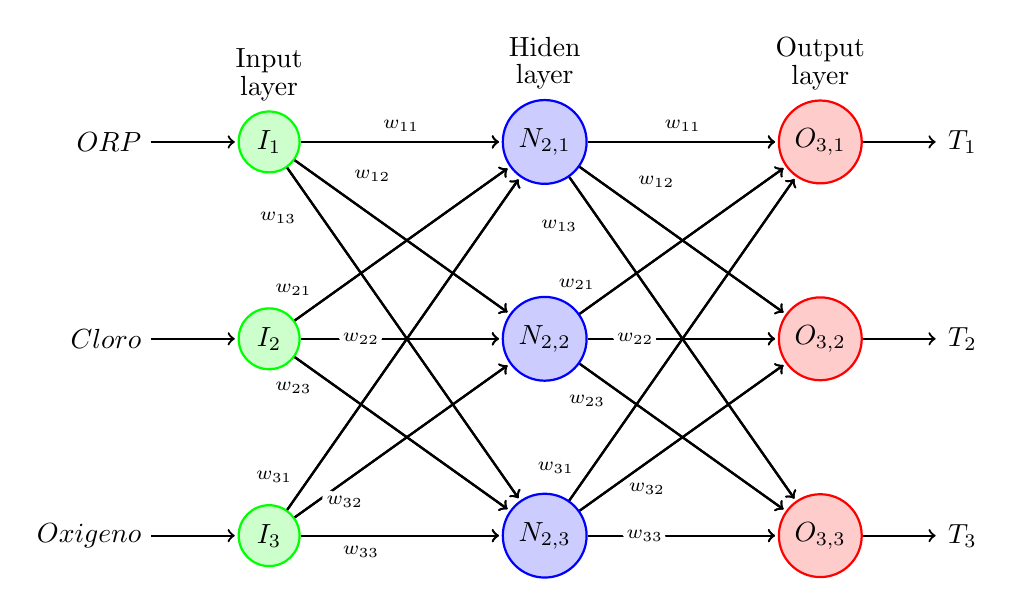
\begin{tikzpicture}[x=3.5cm,y=2.5cm]
	\readlist\Nnod{3,3,3} % number of nodes per layer
	% \Nnodlen = length of \Nnod (i.e. total number of layers)
	% \Nnod[1] = element (number of nodes) at index 1
	\foreachitem \N \in \Nnod{ % loop over layers
	  % \N     = current element in this iteration (i.e. number of nodes for this layer)
	  % \Ncnt  = index of current layer in this iteration
	  \foreach \i [evaluate={\x=\Ncnt; \y=\N/2-\i+1.5; \prev=int(\Ncnt-1);}] in {1,...,\N}{ % loop over nodes
	  \ifnum\x=1
	  \node[input] (N\Ncnt-\i) at (\x,\y) {$I_{\i}$};
  \else\ifnum \x=\Nnodlen
  \node[output] (N\Ncnt-\i) at (\x,\y) {$O_{\x,\i}$};
  \else\ifnum \x>1
  \node[neuron] (N\Ncnt-\i) at (\x,\y) {$N_{\x,\i}$};
  \fi 
  \fi     
  \fi
  
		\ifnum\Ncnt>1 % connect to previous layer
		  \foreach \j in {1,...,\Nnod[\prev]}{ % loop over nodes in previous layer
			\draw[connect] (N\prev-\j) -- (N\Ncnt-\i); % connect arrows directly
		  }
		\fi % else: nothing to connect first layer
	  }
	}
	\node[above,align=center] at (N1-1.90) {Input\\[-0.2em]layer};
	\node[above,align=center] at (N2-1.90) {Hiden\\[-0.2em]layer};
	\node[above,align=center] at (N3-1.90) {Output\\[-0.2em]layer};
	%\draw[connect] (N2-2) -- (N3-1) node[pos=0.50]{\contour{white}{$w{1,1}$}};

	% inputs nodes
	\node[left=1.5cm] (in1) at (N1-1) {$ORP$};
	\node[left=1.5cm] (in2) at (N1-2) {$Cloro$};
	\node[left=1.5cm] (in3) at (N1-3) {$Oxigeno$};
	% outputs nodes
	\node[right=1.5cm] (out1) at (N3-1) {$T_1$};
	\node[right=1.5cm] (out2) at (N3-2) {$T_2$};
	\node[right=1.5cm] (out3) at (N3-3) {$T_3$};
  
  %in/out connections
	\contourlength{0.2em}
	\draw[connect] (in1) -- (N1-1) node[pos=0.50]{\contour{white}{}};
	\draw[connect] (in2) -- (N1-2) node[pos=0.50]{\contour{white}{}};
	\draw[connect] (in3) -- (N1-3) node[pos=0.50]{\contour{white}{}};
	
	\draw[connect] (N3-1) -- (out1) node[pos=0.50]{\contour{white}{}};
	\draw[connect] (N3-2) -- (out2) node[pos=0.50]{\contour{white}{}};
	\draw[connect] (N3-3) -- (out3) node[pos=0.50]{\contour{white}{}};
	
	% Weight connections:
  %  Wih:  [[-0.34583716  0.2400497  -0.23668498]
  %   [ 0.03373939 -0.48542504  0.41874701]
  %   [ 0.40071485 -0.46657857  0.45694934]]
  
	%% input 1
	\draw[connect] (N1-1) -- (N2-1) node[above,pos=0.50]{\contour{white}{\scriptsize $w_{11}$}}; %w11
	\draw[connect] (N1-1) -- (N2-2) node[right=0.1,pos=0.1]{\contour{white}{\scriptsize $w_{12}$}}; %w12
	\draw[connect] (N1-1) -- (N2-3) node[left=0.2cm,pos=0.15]{\contour{white}{\scriptsize $w_{13}$}}; %w13

	%% input 2
	\draw[connect] (N1-2) -- (N2-1) node[left=0.2cm,pos=0.20]{\contour{white}{\scriptsize $w_{21}$}}; % w21
	\draw[connect] (N1-2) -- (N2-2) node[align=center,pos=0.30]{\contour{white}{\scriptsize $w_{22}$}}; %w22
	\draw[connect] (N1-2) -- (N2-3) node[left=0.2cm,pos=0.20]{\contour{white}{\scriptsize $w_{23}$}}; %w23
	  
	%%input 3
	 \draw[connect] (N1-3) -- (N2-1) node[left=0.1cm,pos=0.10]{\contour{white}{\scriptsize $w_{31}$}}; %w31
	\draw[connect] (N1-3) -- (N2-2) node[right=0.cm,pos=0.10]{\contour{white}{\scriptsize $w_{32}$}}; %w32 
	\draw[connect] (N1-3) -- (N2-3) node[below,pos=0.30]{\contour{white}{\scriptsize $w_{33}$}};  %w33
	
  %Who:  [[-0.36279068 -0.21617165  0.10608318]
  % [ 0.44422514  0.35273554 -0.49774077]
  % [ 0.02122603  0.05203763 -0.01462259]]
	
   %% hidden 1
	\draw[connect] (N2-1) -- (N3-1) node[above,pos=0.50]{\contour{white}{\scriptsize $w_{11}$}}; %w11
	\draw[connect] (N2-1) -- (N3-2) node[right=0.1,pos=0.1]{\contour{white}{\scriptsize $w_{12}$}}; %w12
	\draw[connect] (N2-1) -- (N3-3) node[left=0.2cm,pos=0.15]{\contour{white}{\scriptsize $w_{13}$}}; %w13
	
   %% hidden 2
	\draw[connect] (N2-2) -- (N3-1) node[left=0.2cm,pos=0.20]{\contour{white}{\scriptsize $w_{21}$}}; %w21
	\draw[connect] (N2-2) -- (N3-2) node[align=center,pos=0.25]{\contour{white}{\scriptsize $w_{22}$}}; %w22
	\draw[connect] (N2-2) -- (N3-3) node[left=0.2cm,pos=0.25]{\contour{white}{\scriptsize $w_{23}$}}; %w23
	
	%%hidden 3
	 \draw[connect] (N2-3) -- (N3-1) node[left=0.1cm,pos=0.10]{\contour{white}{\scriptsize $w_{31}$}}; %w31
	\draw[connect] (N2-3) -- (N3-2) node[right=0.1cm,pos=0.15]{\contour{white}{\scriptsize $w_{32}$}}; %w32
	\draw[connect] (N2-3) -- (N3-3) node[align=center,pos=0.30]{\contour{white}{\scriptsize $w_{33}$}}; %w33

	%\label{fig:figura_RED}
	
  \end{tikzpicture}
\end{figure}

El tipo de red neuronal generada es de tipo \textit{fully connected}, es decir, cada una de las señales de salida de la capa de entrada lleva una conexión con cada nodo de la capa oculta siguiente; cada señal de salida 
de cada nodo de una capa oculta tiene conexión con todos los nodos de la siguiente capa oculta, o en su respectivo caso, con todos los nodos de la capa de salida de la red.

\clearpage
 % Appendix A
\chapter{Programación del Equipo Wi-Fi Pool Kit de Atlas Scientific}

El código implementado para el funcionamiento del equipo Wi-Fi Pool Kit en los muestreos realizados es el siguiente.

\begin{lstlisting}[language=C++]
    #include <iot_cmd.h>
    #include <WiFi.h>   // Include WiFi library 
    #include "ThingSpeak.h" // Include thingspeak library
    #include <sequencer4.h>  
    #include <sequencer1.h>  
    #include <Ezo_i2c_util.h> // I2C Modules 
    #include <Ezo_i2c.h>    // I2C Modules
    #include <Wire.h>

    WiFiClient client; // This device connects to a Wi-Fi network

    // Wi-Fi Credentials
    const String ssid = "sedeam"; // Name of the Wi-Fi network
    const String pass = "Sede@m2025"; // WiFi password
    const long myChannelNumber = 2399780; // Thingspeak channel number
    const char * myWriteAPIKey = "4SYBSZ1SZKPDQ8RD";    // ThingSpeak API Key

    // Create objects for boards
    Ezo_board DO = Ezo_board(97, "DO"); // DO circuit object, address is 97 and name is "DO"
    Ezo_board ORP = Ezo_board(98, "ORP");   // ORP circuit object, address is 98 and name is "ORP"
    Ezo_board RTD = Ezo_board(102, "RTD");  // RTD circuit object, address is 102 and name is "RTD"
    Ezo_board PMPL = Ezo_board(109, "PMPL");    // PMPL circuit object, address is 109 and name is "PMPL"
    Ezo_board EC = Ezo_board(100, "EC");    // EC circuit object, address is 100 and name is "EC"
    
    // Array of boards used for sending commands to specific boards
    Ezo_board device_list[] = {DO,ORP,RTD,EC,PMPL};

    Ezo_board* default_board = &device_list[0];

    const uint8_t device_list_len = sizeof(device_list) / sizeof(device_list[0]);

    // Enable pins for each circuit
    const int EN_DO = 12;
    const int EN_ORP = 27;
    const int EN_RTD = 15;
    const int EN_AUX = 33;

    const unsigned long reading_delay = 1000;   // How long we wait to receive a response, in milliseconds
    const unsigned long thingspeak_delay = 15000;   // How long we wait to send values to thingspeak, in milliseconds

    unsigned int poll_delay = 2000 - reading_delay * 2 - 300;

    #define PUMP_BOARD        PMPL
    #define PUMP_DOSE         10
    #define EZO_BOARD         DO        
    #define IS_GREATER_THAN   true      
    #define COMPARISON_VALUE  10

    float k_val = 0;    // Holds the k value for determining what to print in the help menu

    bool polling  = true;   // Variable to determine whether or not were polling the circuits
    bool send_to_thingspeak = true; // Variable to determine whether or not were sending data to thingspeak

    // Function to check if wifi is connected
    bool wifi_isconnected() 
    {                           
        return (WiFi.status() == WL_CONNECTED);
    }

    // Function to reconnect wifi if its not connected
    void reconnect_wifi() 
    {                                   
        if (!wifi_isconnected()) 
        {
            WiFi.begin(ssid.c_str(), pass.c_str());
            Serial.println("connecting to wifi");
        }
    }

    void thingspeak_send() 
    {
        if (send_to_thingspeak == true) 
        {                                                    
            if (wifi_isconnected()) 
            {
                int return_code = ThingSpeak.writeFields(myChannelNumber, myWriteAPIKey);
                if (return_code == 200) 
                {
                    Serial.println("sent to thingspeak");
                } 
                else 
                {
                    Serial.println("couldnt send to thingspeak");
                }
            }
        }
    }

    void step1();
    void step2();
    void step3();
    void step4();
    Sequencer4 Seq(&step1,reading_delay,&step2, 300,&step3, reading_delay,&step4, poll_delay);

    Sequencer1 Wifi_Seq(&reconnect_wifi, 10000);

    Sequencer1 Thingspeak_seq(&thingspeak_send, thingspeak_delay);  // Sends data to thingspeak with the time determined by thingspeak delay

    void setup() 
    {
        // Set enable pins as outputs
        pinMode(EN_DO, OUTPUT);                                                         
        pinMode(EN_ORP, OUTPUT);
        pinMode(EN_RTD, OUTPUT);
        pinMode(EN_AUX, OUTPUT);
        // Set enable pins to enable the circuits
        digitalWrite(EN_DO, LOW);                
        digitalWrite(EN_ORP, LOW);
        digitalWrite(EN_RTD, HIGH);
        digitalWrite(EN_AUX, LOW);

        Wire.begin();       
        Serial.begin(9600); // Serial communication to the computer

        WiFi.mode(WIFI_STA);         
        ThingSpeak.begin(client); 
        Wifi_Seq.reset();         
        Seq.reset();
        Thingspeak_seq.reset();
    }

    void loop() 
    {
        String cmd;
        Wifi_Seq.run();
        if (receive_command(cmd)) 
        {
            polling = false;
            send_to_thingspeak = false;
            if (!process_coms(cmd)) 
            {
                process_command(cmd, device_list, device_list_len, default_board);
            }
        }

        if (polling == true) 
        {
            Seq.run();
            Thingspeak_seq.run();
        }
    }

    // Function that controls the pumps activation and output
    void pump_function(Ezo_board &pump, Ezo_board &sensor, float value, float dose, bool greater_than) 
    {
        if (sensor.get_error() == Ezo_board::SUCCESS) 
        {
            bool comparison = false;
            if (greater_than) 
            {
                comparison = (sensor.get_last_received_reading() >= value);
            } 
            else 
            {
                comparison = (sensor.get_last_received_reading() <= value);
            }

            if (comparison) 
            {
                pump.send_cmd_with_num("d,", dose);
                delay(100);
                Serial.print(pump.get_name());
                Serial.print(" ");
                char response[20];
                if (pump.receive_cmd(response, 20) == Ezo_board::SUCCESS) 
                {
                    Serial.print("pump dispensed ");
                } 
                else 
                {
                    Serial.print("pump error ");
                }

                Serial.println(response);
            } 
            else 
            {
                pump.send_cmd("x");
            }
        }
    }

    void step1() 
    {
        // Send a read command
        RTD.send_read_cmd();
    }

    void step2() 
    {
        RTD.receive_read_cmd();
        print_success_or_error(RTD, String(RTD.get_last_received_reading(), 2).c_str());
        
        // If the temperature reading has been received and it is valid
        if ((RTD.get_error() == Ezo_board::SUCCESS) && (RTD.get_last_received_reading() > -1000.0)) 
        
        {
            DO.send_cmd_with_num("T,", RTD.get_last_received_reading());
            EC.send_cmd_with_num("T,", RTD.get_last_received_reading());
            ThingSpeak.setField(1, String(RTD.get_last_received_reading(), 2)); // Assign temperature readings to the first column of thingspeak channel
        } 
        else 
        {
            // If the temperature reading is invalid
            DO.send_cmd_with_num("T,", 20.0);
            EC.send_cmd_with_num("T,", 25.0);   // Send default temp = 25 deg C to PH sensor
            ThingSpeak.setField(1, String(25.0, 2));    // Assign temperature readings to the first column of thingspeak channel
        }

        Serial.print(",");
    }

    void step3() 
    {
        // Send a read command.
        DO.send_read_cmd();
        ORP.send_read_cmd();
        EC.send_read_cmd();
    }

    void step4() 
    {
        DO.receive_read_cmd();
        print_success_or_error(DO, String(DO.get_last_received_reading(), 2).c_str());
        
        if (DO.get_error() == Ezo_board::SUCCESS) 
        {
            ThingSpeak.setField(2, String(DO.get_last_received_reading(), 2));  // Assign PH readings to the second column of thingspeak channel
        }

        Serial.print(",");
        
        ORP.receive_read_cmd();
        print_success_or_error(ORP, String(ORP.get_last_received_reading(), 2).c_str());

        // If the ORP reading was successful
        if (ORP.get_error() == Ezo_board::SUCCESS) 
        {
            ThingSpeak.setField(3, String(ORP.get_last_received_reading(), 0)); // Assign ORP readings to the third column of thingspeak channel
        }

        Serial.print(",");

        EC.receive_read_cmd();
        print_success_or_error(EC, String(EC.get_last_received_reading(), 2).c_str());
        
        if (EC.get_error() == Ezo_board::SUCCESS)
        {
            ThingSpeak.setField(4, String(EC.get_last_received_reading(), 0));
        }

        Serial.println();
        pump_function(PUMP_BOARD, EZO_BOARD, COMPARISON_VALUE, PUMP_DOSE, IS_GREATER_THAN);
    }

    void start_datalogging() 
    {
        polling = true;
        send_to_thingspeak = true;
        Thingspeak_seq.reset();
    }

    bool process_coms(const String &string_buffer) 
    {
        if (string_buffer == "HELP") 
        {
            print_help();
            return true;
        }
        else if (string_buffer.startsWith("DATALOG")) 
        {
            start_datalogging();
            return true;
        }
        else if (string_buffer.startsWith("POLL")) 
        {
            polling = true;
            Seq.reset();
            int16_t index = string_buffer.indexOf(',');
            
            if (index != -1) 
            {
                float new_delay = string_buffer.substring(index + 1).toFloat();
                float mintime = reading_delay * 2 + 300;
                
                if (new_delay >= (mintime / 1000.0)) 
                {
                    Seq.set_step4_time((new_delay * 1000.0) - mintime);
                } 
                else 
                {
                    Serial.println("delay too short");
                }

            }

            return true;

        }

        return false;
    }

    void print_help() 
    {
        Serial.println(F("Atlas Scientific I2C pool kit"));
        Serial.println(F("Commands:"));
        Serial.println(F("datalog      Takes readings of all sensors every 15 sec send to thingspeak "));
        Serial.println(F("             Entering any commands stops datalog mode."));
        Serial.println(F("poll         Takes readings continuously of all sensors"));
        Serial.println(F("                                                                           "));
        Serial.println(F("ph:cal,mid,7     calibrate to pH 7                                         "));
        Serial.println(F("ph:cal,low,4     calibrate to pH 4                                         "));
        Serial.println(F("ph:cal,high,10   calibrate to pH 10                                        "));
        Serial.println(F("ph:cal,clear     clear calibration                                         "));
        Serial.println(F("                                                                           "));
        Serial.println(F("orp:cal,225          calibrate orp probe to 225mV                          "));
        Serial.println(F("orp:cal,clear        clear calibration                                     "));
        Serial.println(F("                                                                           "));
        Serial.println(F("rtd:cal,t            calibrate the temp probe to any temp value            "));
        Serial.println(F("                     t= the temperature you have chosen                    "));
        Serial.println(F("rtd:cal,clear        clear calibration                                     "));
    }
    
\end{lstlisting}

Las primeras 8 líneas del código son la importación de los archivos de encabezado que vienen incluidos en la descarga de las librerías del sitio web de Atlas Scientific, ya que la mayor parte de las funciones llamadas a 
lo largo del código son desarrolladas por el fabricante en lenguaje C++.

Al ser un equipo con la capacidad de conexión a internet y comunicación con la plataforma en línea ThingSpeak de almacenamiento de datos recolectados a nivel remoto, en las líneas de código 12 a 16 se especifican tanto las 
contraseñas y nombre de la red de internet usadas en el laboratorio, así como los identificadores de usuario creados en dicha plataforma. Inicialmente en los primeros muestreos sí se hacía uso de esta herramienta ThingSpeak 
para almacenar la información recolectada, sin embargo, posteriormente se hicieron modificaciones al código para prescindir de esta plataforma y poder recolectar una mayor cantidad de datos debido a que los tiempos de retardo 
para poder enviar los datos a la plataforma hacía que fuera pequeña la cantidad de datos guardados. Por lo tanto, se generaron cambios en el código para poder imprimir los datos muestrados en la terminal del IDE Arduino, lo 
cual permitió poder recolectar mayor cantidad de valores dado que ya no se tenían los tiempo de espera necesarios de comunicación entre el equipo Pool Kit y la plataforma ThingSpeak.

Esta implementación está desarrollada bajo la metodología de Programación Orientada a Objetos; en las líneas de código 18 a 23 se inicializan objetos de tipo \textit{Ezo Board}, los cuales permiten crear un tipo de identificador 
para cada una de los circuitos de acondicionamiento de señal correspondiente a 1 de los parámetros muestreados; estos objetos reciben como parámetros de inicio el nombre que corresponde a la variable específica, además del 
valor numérico que corresponde a la dirección usada en la comunicación I2C entre los circuitos y microcontrolador, para que el microcontrolador pueda diferenciar entre los diferentes circuitos.

En las líneas 32 a 36 del código se declaran los valores numéricos de los pines del microcontrolador que estarán conectados con los circuitos de instrumentación de señal; en este caso, el circuito de oxígeno disuelto se 
conecta con el pin 12, el circuito de ORP con el pin 27, el circuito de temperatura va al pin número 15, y finalmente el circuito auxiliar restante se conecta al pin 33 del microcontrolador. Posteriormente, en las líneas 
38 y 39 de código se declaran los valores de los tiempos de espera usados para la comunicación entre la plataforma ThingSpeak y el equipo Pool Kit.

En la línea 55 de código se declara la función \textit{WifiIsConnected} que continuamente se encarga de verificar que haya conexión de internet estable en el equipo cuando se están enviando datos a la plataforma ThingSpeak.
Posteriormente, en la línea 61 a 68 de código la función \textit{reconnect wifi} se encarga de reestablecer la conexión a internet en caso de que previamente se haya detectado que se ha perdido. En las líneas 70 a 87 del 
código se declara la función \textit{thingspeak send} que se encarga de mostrar mensajes en terminal sobre el estado de la comunicación entre el equipo Pool Kit y la plataforma, específicamente informar al usuario si ha 
existido algún registro de datos muestreado que no ha podido ser enviado a la plataforma y por lo tanto se ha perdido.

En las líneas 89 a 93 de código se declaran los encabezados de las funciones \textit{step}, las cuales en su estructura, que se define en líneas posteriores del código, presentan los procedimientos generados para la lectura 
de las señales obtenidas por los sensores, así como su procesamiento, para finalmente poder obtener un valor numérico que represente la magnitud medida para los parámetros muestreados, ya que los sensores únicamente generan
pequeños voltajes eléctricos que deben ser convertidos a su equivalente magnitud para las variables muestreadas.

En las líneas de código 100 a 120 se escribe la función \textit{setup} que en los entornos Arduino sirve para realizar la configuración inicial del microcontrolador, la cual se ejecuta sólo 1 vez. En esta función se habilitan 
los pines de la tarjeta que tienen conexión con los circuitos de instrumentación para poder generar la comunicación necesaria para obtener las señales que representan los parámetros muestreados. Igualmente, en esta función 
\textit{setup} también se hacen llamadas a las funciones encargadas de iniciar la conexión a internet y la sincronización con la plataforma ThingSpeak cuando se desea hacer almacenamiento en línea de las información recolectada.

En las líneas de código 122 a 141 se escribe la función \textit{loop} que en los entornos Arduino es la que se ejecuta repetidamente logrando así el funcionamiento continuo de la tarjeta de microcontrolador. En este caso, 
internamente la función \textit{loop} contiene las llamadas a las funciones \textit{step} que se encargan de extraer las señales eléctricas de las sondas para poder hacer los cálculos necesarios y obtener las magnitudes 
numéricas de los parámetros estudiados. Al tener las funciones \textit{step} dentro de la función \textit{loop} nos aseguramos de que la recolección, almacenamiento e impresión de los datos en terminal se realicen de forma 
ininterrumpida.

En la línea 183 de código se presenta la estructura de la función \textit{step1}, la cual es 1 de las 4 funciones base para el funcionamiento secuencial del equipo Pool Kit. En esta caso, \textit{step1} se encarga de ejecutar 
un llamado a otra función que pide que se inicie la lectura de un dato de la variable de temperatura. Esto es indispensable que sea el primer paso llevado a cabo para un muestreo individual de los 4 parámetros disponibles 
en el equipo, ya que la temperatura es factor que influye en las mediciones hechas para los otros sensores, por lo cual es importante que el primer dato recolectado sea la temperatura. De esta forma, al tener el valor de la 
temperatura actual, al calcular los valores numéricos para las señales de los otros sensores es posible usar el valor de temperatura para realizar la compensación necesaria en los cálculos de las otras variables.

En la línea 189 de código se inicia la estructura de la función \textit{step2}, en la cual se recibe el dato numérico del valor de temperatura actual y se imprime en la terminal del IDE Arduino. Además de lo anterior, dicho 
valor actual de temperatura es almacenado temporalmente para poder realizar compensación para los sensores de oxígeno disuelto y conductividad eléctrica, en caso de que dichos sensores estén conectados al equipo para medición 
de dichos parámetros. Por último, en esta función también se hace el envío a la plataforma ThingSpeak del primer valor correspondiente a un registro de datos, que en este caso viene siendo la temperatura y faltaría el envío 
de otros 3 datos numéricos adicionales para completar 1 registro que correspondería a 1 muestreo individual.

En la línea 213 de código, se presenta la estructura de la función \textit{step3}, en la cual se hacen llamados a funciones externas para poder iniciar la lectura de los otros 3 sensores disponibles, que para este caso serían 
oxígeno disuelto, ORP y conductividad eléctrica. Posteriormente en la línea 221 del código, se inicia la estructura de la función \textit{step4}, la cual es la última en el funcionamiento secuencial ininterrupmido del equipo 
Pool Kit. En esta última función, lo que se realiza es el envío a la plataforma ThingSpeak de los datos de los 3 parámetros restantes, además de generar su impresión en la terminal del Arduino IDE.

Finalmente, en la última parte del código a partir de la línea 304 se desarrolla la función \textit{print help} la cual permite imprimir en la terminal del Arduino IDE los comandos de ayuda para el usuario acerca del manejo 
del equipo Pool Kit durante su funcionamiento. Al ser invocada esta función por el usuario desde la terminal, se imprime información sobre acciones específicas, tales como iniciar el muestreo de manera continua, detener 
el envío de datos a la plataforma ThingSpeak, comandos de calibración para el sensor de potencial de Hidrógeno, comando de calibración para el sensor de ORP y comandos de calibración para el sensor de temperatura.
 % Appendix B
\chapter{Repositorios}

En el siguiente repositorio de github se encuentran los datos de calidad del agua recolectados durante la realización de este proyecto:

\begin{center}
\url{https://github.com/bryanMartinMiranda/Datos_Y_Modelos_2024}, 
\end{center}

El siguiente repositorio contiene el proyecto realizado en \LaTeX\ para la generación de este documento de tesis:

\begin{center}
\url{2024}, 
\end{center}
 % Appendix C
%-=-=-=-=-=-=-=-=-=-=-=-=-
% 4) References
\cleardoublepage
% Bibliography

\label{bibliography} % Reference the bibliography elsewhere with \autoref{bibliography}



\bibliographystyle{IEEEtran}
\bibliography{Reference,Mi_Biblioteca_Protocolo,Referencias_WATER_Quality,importanciaAgua1,sem3_uno,sem3_dos}


%-=-=-=-=-=-=-=-=-=-=-=-=-
% 5) Back Matter
\cleardoublepage
%!TeX root=../thesisStructure.tex
% Colophon: a brief description of publication or production notes relevant to the edition.

\pagestyle{empty}
\hfill
\vfill
\pdfbookmark[0]{Colophon}{Colophon}
\section*{Colophon}

This document was typeset using the  \texttt{itmthesis} class developed by Gerardo Marx Chávez-Campos. The class was designed based on the \texttt{classicthesis} class developed by Andr\'e Miede. The \texttt{itmthesis} is available for \LaTeX\ in a github repository at: 

\begin{center}
\url{https://github.com/MCIE-RS101/itmorelia-protocol-class}, 
\end{center}

this document can be extended to a thesis document. Thus, you can try by yourself or use the \textit{thesis-class} repository at:

\begin{center}
\url{https://gitea.itmorelia.com}, 
\end{center}

\noindent Any further comment, sugestion or if you want to collaborate to improve these  classes please contact me at:

\href{mailto:gmarx\_cc@itmorelia.edu.mx}{gmarx\_cc@itmorelia.edu.mx} 

\section*{Colofón}

Este documento fue generado usando el estilo desarrollado en la clase \texttt{itmthesis}, desarrollada por Gerardo Marx Chávez-Campos. Esta  fue diseñada basada en el estilo \texttt{classicthesis} desarrollado por Andr\'e Miede. 

El estilo \texttt{itmthesis} y un ejemplo de su uso está disponible en repositorios para ser compilados en \LaTeX\ en: 

\begin{center}
\url{https://github.com/MCIE-RS101/itmorelia-protocol-class}, 
\end{center}
este documento puede ser extendido a uno de tesis. Por lo tanto, puedes tratar de hacerlo por ti mismo, o usar el repositorio en:

\begin{center}
\url{https://gitea.itmorelia.com}, 
\end{center}

\noindent Cualquier comentario, sugerencia, o si deseas colaborar en mejorar estos estilos por favor contacta me en:

\href{mailto:gmarx\_cc@itmorelia.edu.mx}{gmarx\_cc@itmorelia.edu.mx} 
%-=-=-=-=-=-=-=-=-=-=-=-=-
\end{document}
%%% Local Variables:
%%% mode: latex
%%% TeX-master: t
%%% End: